%%%%%%%%%%%%%%%%%%%%%%%%%%%%%%%%%%%%%%%%%%%%%%%%%%%%%%%%%%%%%%%%%%%%%%%%%%%%%%%
%% Trabalho de Conclusão de Curso: detecção de falhas em máquinas industriais (Kaelix)
%% Modelo do iCEV em abnTeX2 (preambulo/estilo-icev.tex), com a organização em seis capítulos,
%% os números gerados por script (values/) e as hipóteses registradas antes do cálculo.
%% Compilar: make (pdflatex, bibtex, makeglossaries, makeindex, pdflatex, pdflatex), saída em build/.
%%%%%%%%%%%%%%%%%%%%%%%%%%%%%%%%%%%%%%%%%%%%%%%%%%%%%%%%%%%%%%%%%%%%%%%%%%%%%%%

\documentclass[
	12pt,
	openright,
	oneside,
	a4paper,
	chapter=TITLE,
	english,
	brazil
	]{abntex2}

%%%%%%%%%%%%%%%%%%%%%%%%%%%%%%%%%%%%%%%%%%%%%%%%%%%%%%%%%%%%%%%%%%%%%%%%%%%%%%%
%% Pacotes do documento
%%
%% Os do modelo iCEV (indentfirst, abntex2cite) e os que o conteúdo
%% exige (siunitx, glossaries, nomencl, booktabs). A ordem importa:
%%   glossaries depois do hyperref, que a abntex2 carrega.
%%%%%%%%%%%%%%%%%%%%%%%%%%%%%%%%%%%%%%%%%%%%%%%%%%%%%%%%%%%%%%%%%%%%%%%%%%%%%%%

%% --- Fontes e codificação --------------------------------------------------
\usepackage[T1]{fontenc}
\usepackage[utf8]{inputenc}
\usepackage{indentfirst}
%% Times no corpo, como no modelo. O modelo usa mathptmx; newtx compõe a mesma
%% Times com matemática completa (negrito, letras gregas), que os capítulos
%% usam. As figuras do pipeline (experiments/figures/scripts/theme_kaelix.R)
%% compõem em Times New Roman para casar com este corpo.
\usepackage{newtxtext,newtxmath}
\usepackage{microtype}

%% --- Pacotes de conteúdo ---------------------------------------------------
\usepackage{graphicx}
\usepackage{xcolor}      % marcas vermelhas \emandamento; substitui o color do modelo
\usepackage{booktabs}    % réguas de tabela
\usepackage{amsmath}
\usepackage{caption}
%% Título antes da ilustração ou da tabela (NBR 14724, 5.8 e 5.9).
\captionsetup{justification=justified,singlelinecheck=false}
\captionsetup[figure]{position=top}
\captionsetup[table]{position=top}
\usepackage{letltxmacro} % \LetLtxMacro para o \fonte de estilo-icev.tex
\usepackage{siunitx}
%% Separador decimal do português: vírgula. Sem isto, \num{0,5} sai "0.5".
%% Incerteza: \SI{75,0 \pm 3,5}{\percent} sai "(75,0 ± 3,5) %", com a unidade
%% valendo para os dois números; para "75,0 % ± 3,5 %", troque bracket por repeat.
\sisetup{
  output-decimal-marker      = {,},
  group-separator            = {\,},
  range-phrase               = {~a~},
  list-final-separator       = {~e~},
  per-mode                   = symbol,
  uncertainty-mode           = separate,
  separate-uncertainty-units = bracket
}

%% --- Citações (ABNT, sistema autor-data) -----------------------------------
\usepackage[alf,bibleftalign]{abntex2cite}
%% Estilo local, ajustado à NBR 6023:2025 e à NBR 10520:2023; as alterações
%% estão listadas no topo do arquivo. O abntex2-alf da distribuição segue as
%% normas de 2018 e 2002 e não imprime DOI.
\bibliographystyle{abntex2-alf-2025}
%% A NBR 6023 não usa < > em volta do endereço eletrônico desde 2018; o
%% abntex2cite ainda os acrescenta a todo \url.
\def\UrlLeft{}
\def\UrlRight{}

%% --- Listas de siglas e de símbolos ----------------------------------------
%% Sem as opções que põem as listas no sumário: elementos pré-textuais não podem
%% constar nele (NBR 6027, 6.3).
\usepackage[acronym,nomain,nonumberlist]{glossaries}
\makeglossaries
\usepackage{nomencl}
\makenomenclature

%% --- Caminhos para o repositório -------------------------------------------
%% Definidos uma única vez aqui; os capítulos têm fallback idêntico.
\newcommand{\kxfig}[1]{../../../experiments/figures/output/#1}
\newcommand{\kxhw}[1]{../../../#1}

%%%%%%%%%%%%%%%%%%%%%%%%%%%%%%%%%%%%%%%%%%%%%%%%%%%%%%%%%%%%%%%%%%%%%%%%%%%%%%%
%% Estilo do modelo de monografia do iCEV
%%
%% Transcrito de monografia-tcc/main.tex: fontes de título, logo no cabeçalho,
%% capa, folha de rosto, ambiente de resumo, citação nas referências e cores
%% dos links. Divergências deliberadas do modelo, todas pelas normas ABNT:
%%   - Referências sem indicativo numérico (o modelo as numerava como capítulo).
%%   - Texto preto, inclusive nos links (NBR 14724, 5.1); o modelo usa azul.
%%   - Títulos em corpo 12, graduados por caixa-alta e negrito, com o mesmo destaque
%%     no sumário e no texto (NBR 14724, 5.1 e 5.4; NBR 6027). Por isso as seções
%%     secundárias não usam caixa-alta (sem section=TITLE em main.tex).
%%   - Um espaço entre indicativo e título (NBR 14724, 5.2.2).
%%   - Margem inferior de 2 cm e número da página a 2 cm da borda superior (NBR 14724,
%%     5.1 e 5.3); o modelo chega a cerca de 1,5 cm e a 2,4 cm.
%%   - Introdução em caixa-alta no sumário, como os demais capítulos.
%%   - Sem título corrente no cabeçalho: o logo de 15 cm cobre quase toda a
%%     largura do texto (16 cm) e escondia o título atrás da imagem. A NBR 14724
%%     só exige a paginação no canto superior direito.
%%   - Introdução numerada, como seção primária (NBR 14724, 5.2.3; NBR 6024); o modelo a
%%     deixa sem número. Decisão do usuário, em 2026-11-01.
%%   - Referências alinhadas à esquerda, com título em negrito (NBR 6023).
%% Os dados (título, autor, curso) ficam em preambulo/dados.tex.
%%%%%%%%%%%%%%%%%%%%%%%%%%%%%%%%%%%%%%%%%%%%%%%%%%%%%%%%%%%%%%%%%%%%%%%%%%%%%%%

%% --- Títulos -----------------------------------------------------------------
\renewcommand{\ABNTEXchapterfont}{\rmfamily\bfseries}
\renewcommand{\ABNTEXchapterfontsize}{\normalsize}
\renewcommand{\ABNTEXsectionfontsize}{\normalsize}
\renewcommand{\ABNTEXsubsectionfont}{\rmfamily\mdseries}
\renewcommand{\ABNTEXsubsectionfontsize}{\normalsize}
\setsecnumformat{\csname the#1\endcsname\ }
%% Um espaço entre número e título (NBR 14724, 5.2.2): a definição da classe deixa dois.
\makeatletter
\renewcommand{\printchapternum}{%
	\tocprintchapter
	\setboolean{abntex@innonumchapter}{false}%
	\chapnumfont
	\ifthenelse{\boolean{abntex@apendiceousecao}}%
		{\space\thechapter\tocinnonumchapter\ABNTEXcaptiondelim}%
		{\thechapter\space}%
}
\makeatother
%% Título separado do texto por uma linha em branco de espaço 1,5 (NBR 14724, 5.2.2).
\setlength{\afterchapskip}{0pt}
%% Destaque do sumário igual ao do texto: terciária sem negrito (NBR 14724, 5.4).
\renewcommand{\cftsubsectionfont}{\normalfont\normalsize}
\renewcommand{\cftsubsectionpagefont}{\normalfont\normalsize}
%% Apêndice no sumário: "APÊNDICE A --- TÍTULO".
\cftinsertcode{A}{%
	\renewcommand{\cftchapteraftersnum}{~\textemdash~}%
	\renewcommand{\cftchapterpresnum}{\unskip}%% a classe deixa dois espaços após "APÊNDICE"
}
\renewcommand{\tocinnonumchapter}{%
	%% 2 em cobre "A ---"; o memoir soma a largura de "APÊNDICE", e a segunda linha alinha sob
	%% o início do título.
	\addtocontents{toc}{\cftsetindents{chapter}{\cftlastnumwidth}{2em}}%
	\cftinserthook{toc}{A}%
}
%% O sumário já recebe o espaço que antecede a primeira entrada.
\renewcommand{\aftertoctitle}{\par\vspace{6.3pt}}
\renewcommand{\afterloftitle}{\par\vspace{\baselineskip}}
\renewcommand{\afterlottitle}{\par\vspace{\baselineskip}}
\setbeforesecskip{\baselineskip}
\setaftersecskip{\baselineskip}
\setbeforesubsecskip{\baselineskip}
\setaftersubsecskip{\baselineskip}
%% Equações em numeração corrida, como figuras e tabelas.
\counterwithout{equation}{chapter}

%% --- Notas, ilustrações e tabelas ---------------------------------------------
%% Filete de 5 cm a partir da margem esquerda (NBR 14724, 5.2).
\renewcommand{\footnoterule}{\kern-3pt\hrule width 5cm\kern 2.6pt}
%% Tabela em corpo 12; só fonte, legenda e nota ficam menores (NBR 14724, 5.1).
\renewcommand{\IBGEtabfontsize}{\normalsize}
%% Com o título acima, o caption não deixa espaço antes da fonte.
\LetLtxMacro{\fonteabntex}{\fonte}
\renewcommand{\fonte}[2][\fontename]{\par\vspace{3pt}\fonteabntex[#1]{#2}}
%% Legenda abaixo da fonte (NBR 14724, 5.8); o título vem antes da ilustração.
\newcommand{\legenda}[1]{\nota[Legenda]{#1}}
%% Mesma autoria, datas diferentes: (Autor, 2009, 2022), como pede a NBR 10520, 6.1.
\newcommand{\citemesmoautor}[3]{(#1, \citeyear{#2}, \citeyear{#3})}

%% --- Referências -------------------------------------------------------------
%% Sem "Citado na página" do modelo: a NBR 6023 não prevê esse elemento.
\renewcommand{\bibsection}{%
	\chapter*{\bibname}%
	\addcontentsline{toc}{chapter}{\MakeTextUppercase{\bibname}}%
	\bibmark
	\vspace*{21.4pt}%% uma linha em branco de espaço 1,5 (NBR 14724, 5.2.2)
	\prebibhook
}

%% --- Cabeçalho com logo --------------------------------------------------------
\newcommand{\logoicevheader}{
\includegraphics[width=15cm]{imagens/logo-icev.jpg}}

\makepagestyle{icevpretextual}
\makeevenhead{icevpretextual}{}{\logoicevheader}{}
\makeoddhead{icevpretextual}{}{\logoicevheader}{}
\aliaspagestyle{titlingpage}{icevpretextual}

\makepagestyle{icevheadings}
%% O número sobe para ficar a 2 cm da borda superior (NBR 14724, 5.3).
\newcommand{\icevnumeropagina}{\raisebox{0.35cm}{\ABNTEXfontereduzida\thepage}}
\makeevenhead{icevheadings}{\icevnumeropagina}{\logoicevheader}{}
\makeoddhead{icevheadings}{}{\logoicevheader}{\icevnumeropagina}
\makeheadrule{icevheadings}{\textwidth}{\normalrulethickness}

\makepagestyle{icevchapfirst}
\makeoddhead{icevchapfirst}{}{\logoicevheader}{\icevnumeropagina}

%% O modelo usa 2.1cm, mas o logo mede 60,6pt e não cabe (aviso do memoir e
%% \vbox overfull em toda página). Com 2.15cm cabe, e cabeçalho mais
%% \headsep continuam dentro da margem superior de 3 cm.
\setlength{\headheight}{2.15cm}
\setlength{\headsep}{0.5cm}
\checkandfixthelayout
%% Sem este ajuste, a última linha de uma página cheia fica a cerca de 1,7 cm da borda;
%% a margem inferior é de 2 cm (NBR 14724, 5.1).
\addtolength{\textheight}{-0.5cm}
\checkandfixthelayout[fixed]

%% --- Links ---------------------------------------------------------------------
%% pdftitle e pdfauthor ficam em dados.tex: aqui \@title e \@author ainda estão vazios.
\makeatletter
\hypersetup{
	pdfsubject  = {Trabalho de Conclusão de Curso},
	pdfcreator  = {LaTeX with abnTeX2},
	pdfkeywords = {manutenção preditiva; análise de vibração; detecção de anomalias;
	               sistemas embarcados; instrumentação de baixo custo},
	hidelinks,
	bookmarksdepth = 4
}
\makeatother

%% --- Parágrafo -----------------------------------------------------------------
\setlength{\parindent}{1.25cm}
\setlength{\parskip}{0pt}

%% --- Capa ----------------------------------------------------------------------
\renewcommand{\imprimircapa}{%
	\begin{capa}
		\centering
		{\ABNTEXchapterfont\bfseries\instituicaoicev\par}
		{\ABNTEXchapterfont\bfseries\cursoicev\par}

		\vfill
		{\ABNTEXchapterfont\bfseries\imprimirautor}
		\vfill

		\begin{center}
			\ABNTEXchapterfont\bfseries\imprimirtitulo
		\end{center}
		\vfill

		{\bfseries\imprimirlocal\par}
		{\bfseries\imprimirdata}
		\vspace*{1cm}
	\end{capa}
}

%% --- Natureza do trabalho --------------------------------------------------------
%% Do meio da mancha até a margem direita, em espaço simples, na folha de rosto e na
%% de aprovação (NBR 14724, 5.2).
\newcommand{\icevnatureza}{%
	{\raggedleft
	\begin{minipage}{.5\textwidth}
		\SingleSpacing
		%% Espaços sem encolher: nesta coluna estreita, a linha apertada colava
		%% as palavras ao copiar do PDF. Sem hifenizar o nome da instituição.
		\spaceskip=\fontdimen2\font plus \fontdimen2\font\relax
		\hyphenpenalty=10000
		\imprimirpreambulo
	\end{minipage}\par}%
}

%% --- Folha de rosto ------------------------------------------------------------
\makeatletter
\renewcommand{\folhaderostocontent}{
	\begin{center}

		{\ABNTEXchapterfont\bfseries\imprimirautor}

		\vspace*{\fill}\vspace*{\fill}
		\begin{center}
			\ABNTEXchapterfont\bfseries\imprimirtitulo
		\end{center}
		\vspace*{\fill}

		\abntex@ifnotempty{\imprimirpreambulo}{%
			\icevnatureza
			\vspace*{\fill}
		}%

		{\abntex@ifnotempty{\imprimirinstituicao}{\imprimirinstituicao\vspace*{\fill}}}

		{\imprimirorientadorRotulo~\imprimirorientador\par}
		\abntex@ifnotempty{\imprimircoorientador}{%
			{\imprimircoorientadorRotulo~\imprimircoorientador}%
		}%
		\vspace*{\fill}

		{\bfseries\imprimirlocal}
		\par
		{\bfseries\imprimirdata}
		\vspace*{1cm}

	\end{center}
}
\makeatother

%% --- Resumo --------------------------------------------------------------------
\renewenvironment{resumo}[1][\resumoname]{%
	\PRIVATEbookmarkthis{#1}
	\renewcommand{\abstractnamefont}{\ABNTEXchapterfont\bfseries}
	\renewcommand{\abstractname}{\ABNTEXchapterupperifneeded{#1}}
	\begin{abstract}
}{\end{abstract}\PRIVATEclearpageifneeded}
\setlength{\absparsep}{18pt}
\addtolength{\abstitleskip}{1.7pt}

%% --- Trechos que mudam com as medições do dispositivo --------------------------
%% Definido aqui porque o resumo e o abstract também usam, antes das seções.
\providecommand{\emandamento}[1]{\textcolor{red}{#1}}

%% --- Quadros --------------------------------------------------------------------
%% Quadro é ilustração (NBR 14724, 5.8), com lista própria antes da de tabelas.
\newcommand{\quadroname}{Quadro}
\newcommand{\listofquadrosname}{Lista de quadros}
\newfloat[chapter]{quadro}{loq}{\quadroname}
\newlistof{listofquadros}{loq}{\listofquadrosname}
\newlistentry{quadro}{loq}{0}
\counterwithout{quadro}{chapter}
%% Mesmo separador das tabelas e figuras do abnTeX2 (espaço, meia-risca, espaço).
\captionsetup[quadro]{position=top,labelsep=endash}
%% Separador das legendas nos apêndices, onde \ABNTEXcaptiondelim vira travessão para o título
%% "APÊNDICE A --- TÍTULO"; \kxdelimlegenda guarda o separador do texto (main.tex, apendicesenv).
\DeclareCaptionLabelSeparator{kxlegenda}{\kxdelimlegenda}
\renewcommand{\cftquadroname}{\quadroname\space}
\renewcommand*{\cftquadroaftersnum}{\hfill\textendash\hfill}
\renewcommand{\afterloqtitle}{\par\vspace{\baselineskip}}

%% --- Referências -------------------------------------------------------------
%% Separadas por uma linha em branco de espaço simples (NBR 6023, 6.3).
\setlength{\bibitemsep}{10pt}
%% Data provável, entre colchetes (NBR 6023, 8.6): os colchetes no campo year quebram o
%% argumento opcional de \bibitem, por isso ela fica em uma macro.
\newcommand{\anomafaulda}{[201-?]}

%% --- Listas de siglas e de símbolos ------------------------------------------
%% Mesma separação entre título e texto das demais listas.
\renewcommand*{\glossarypreamble}{\vspace*{\baselineskip}}
\renewcommand{\nompreamble}{\vspace*{20pt}}

%% --- Páginas só de ilustrações -------------------------------------------------
%% Uma página com uma ou mais ilustrações e sem texto começa no topo, em vez de deixar
%% a ilustração centralizada no meio da página com espaço vazio acima.
\makeatletter
\setlength{\@fptop}{0pt}
\setlength{\@fpsep}{\floatsep}
\setlength{\@fpbot}{0pt plus 1fil}
\makeatother

%%%%%%%%%%%%%%%%%%%%%%%%%%%%%%%%%%%%%%%%%%%%%%%%%%%%%%%%%%%%%%%%%%%%%%%%%%%%%%%
%% Dados do trabalho
%%%%%%%%%%%%%%%%%%%%%%%%%%%%%%%%%%%%%%%%%%%%%%%%%%%%%%%%%%%%%%%%%%%%%%%%%%%%%%%

%% Título definido pelo autor em 08/11/2026, entre as alternativas de uma pesquisa
%% sobre títulos (NBR 14724:2024, 4.1.1 c e d; guia de redação da USC; estudos
%% sobre tamanho e tipo de título). O título nomeia o objeto e o método; o
%% subtítulo, depois de dois-pontos, nomeia a operação feita (avaliação) e o
%% objeto avaliado (o sistema). Sem resultado, sem sigla e sem nome de projeto.
%% A quebra depois dos dois-pontos separa título e subtítulo nas três folhas; nos
%% metadados do PDF ela vira espaço.
\titulo{Detecção de falhas em máquinas industriais por afastamento da operação normal:\texorpdfstring{\\}{ }avaliação de um sistema de baixo custo}
\autor{Lauan Matheus da Rocha Alves}
\local{Teresina -- PI}
\data{2026}
\orientador[Orientadora:]{Lia Mariana Nascimento Brito}
%\coorientador{Nome do coorientador}
\preambulo{Trabalho de Conclusão de Curso apresentado como requisito parcial
para obtenção do título de Bacharel em Engenharia de Software do Instituto de
Ensino Superior -- iCEV.}

%% Metadados do PDF: precisam vir depois de \titulo e \autor.
\makeatletter
\hypersetup{pdftitle = {\@title}, pdfauthor = {\@author}}
\makeatother

%% Usados na capa do modelo iCEV (preambulo/estilo-icev.tex).
\newcommand{\cursoicev}{Curso de Bacharelado em Engenharia de Software}
\newcommand{\instituicaoicev}{Instituto de Ensino Superior -- iCEV}


\graphicspath{{Images/}{../../../experiments/figures/output/}}

%% Números do texto, gerados por script. Não digitar números da coleta no texto.
%%   campo_values.tex       scripts/build_field_values.py (dados exportados da coleta)
%%   hipoteses_values.tex   experiments/campo/analise_registrada.py (H1 a H3, registro_v1)
%%   descritivos_values.tex experiments/campo/analise_descritiva.py
%%   resultados_values.tex  scripts/build_results_values.py (detalhes lidos dos CSV)
%%   posterior_values.tex   experiments/campo/analise_posterior.py (AP1 e AP2, registro_v2)
%%   h4_values.tex          experiments/fraunhofer/analise_h4.py (H4, registros v2 e v3)
%%   dados_values.tex       scripts/build_dados_values.py (versões do ambiente, citadas na seção de análise estatística)
%%   tabelas_ensaio_values.tex scripts/build_tabelas_ensaio.py (tabelas do apêndice de dados por ensaio)
%%   sistema_values.tex     scripts/build_sistema_values.py (capítulo do sistema: código, testes e ensaios de 2/11)
% Gerado por scripts/build_field_values.py; não editar à mão.
\newcommand{\campoBuscaCalandraDois}{29,8}
\newcommand{\campoBuscaCalandraUm}{29,8}
\newcommand{\campoBuscaCompressorUm}{59,8}
\newcommand{\campoBuscaDobradeiraUm}{29,8}
\newcommand{\campoBuscaGuilhotinaDois}{30,0}
\newcommand{\campoBuscaGuilhotinaUm}{30,0}
\newcommand{\campoCicloDois}{11}
\newcommand{\campoCicloUm}{15}
\newcommand{\campoCoberturaDois}{4,7}
\newcommand{\campoCoberturaUm}{3,4}
\newcommand{\campoDesvioTaxaMax}{0,16}
\newcommand{\campoEnsaios}{6}
\newcommand{\campoFimCalandraDois}{15h55}
\newcommand{\campoFimCalandraUm}{13h25}
\newcommand{\campoFimCompressorUm}{13h48}
\newcommand{\campoFimDobradeiraUm}{13h00}
\newcommand{\campoFimGuilhotinaDois}{16h06}
\newcommand{\campoFimGuilhotinaUm}{13h08}
\newcommand{\campoFimMotorParado}{13h14}
\newcommand{\campoInicioCalandraDois}{15h47}
\newcommand{\campoInicioCalandraUm}{13h18}
\newcommand{\campoInicioCompressorUm}{13h40}
\newcommand{\campoInicioDobradeiraUm}{12h48}
\newcommand{\campoInicioGuilhotinaDois}{16h00}
\newcommand{\campoInicioGuilhotinaUm}{13h05}
\newcommand{\campoInicioMotorParado}{13h11}
\newcommand{\campoIntervaloCalandra}{2~h~29~min}
\newcommand{\campoIntervaloGuilhotina}{2~h~55~min}
\newcommand{\campoJanelas}{218}
\newcommand{\campoJanelasCalandraDois}{47}
\newcommand{\campoJanelasCalandraUm}{25}
\newcommand{\campoJanelasCompressorUm}{33}
\newcommand{\campoJanelasDobradeiraUm}{50}
\newcommand{\campoJanelasGuilhotinaDois}{35}
\newcommand{\campoJanelasGuilhotinaUm}{13}
\newcommand{\campoJanelasMotorParado}{15}
\newcommand{\campoJanelasOperacao}{203}
\newcommand{\campoJanelasRepouso}{238}
\newcommand{\campoLacunas}{0}
\newcommand{\campoLacunasTexto}{não teve nenhuma lacuna}
\newcommand{\campoLeituras}{218}
\newcommand{\campoMaquinas}{4}
\newcommand{\campoPotenciaTx}{17}
\newcommand{\campoRajadas}{862}
\newcommand{\campoRajadasFim}{16h07}
\newcommand{\campoRajadasInicio}{13h14}
\newcommand{\campoRepousoFim}{14h59}
\newcommand{\campoRepousoInicio}{14h00}
\newcommand{\campoRmsCalandraDois}{321,5}
\newcommand{\campoRmsCalandraUm}{304,9}
\newcommand{\campoRmsCompressorUm}{214,4}
\newcommand{\campoRmsDobradeiraUm}{218,3}
\newcommand{\campoRmsGuilhotinaDois}{33,3}
\newcommand{\campoRmsGuilhotinaUm}{37,1}
\newcommand{\campoRmsMotorParado}{3,3}
\newcommand{\campoRssiMax}{\textminus 68}
\newcommand{\campoRssiMin}{\textminus 105}
\newcommand{\campoTaxaMax}{1000,51}
\newcommand{\campoTaxaMin}{998,37}
\newcommand{\campoTempCalandraDois}{74,1}
\newcommand{\campoTempCalandraUm}{41,6}
\newcommand{\campoTempCompressorUm}{43,3}
\newcommand{\campoTempDobradeiraUm}{44,0}
\newcommand{\campoTempGuilhotinaDois}{72,8}
\newcommand{\campoTempGuilhotinaUm}{43,8}
\newcommand{\campoTempMotorParado}{44,2}
\newcommand{\campoTempRodadaDoisMax}{74,1}
\newcommand{\campoTempRodadaDoisMin}{72,8}
\newcommand{\campoTempRodadaUmMax}{44,0}
\newcommand{\campoTempRodadaUmMin}{41,6}
\newcommand{\registroDoisShaCurto}{3246d219}
\newcommand{\registroExplIfMax}{23}
\newcommand{\registroExplIfMin}{0}
\newcommand{\registroExplMadMax}{38}
\newcommand{\registroExplMadMin}{0}
\newcommand{\registroShaCurto}{fd0afc89}
\newcommand{\registroTresShaCurto}{9197884e}

% Gerado por experiments/campo/analise_registrada.py; não editar à mão.
\newcommand{\hDoisMmdMax}{3,20}
\newcommand{\hDoisMmdMin}{0,55}
\newcommand{\hDoisVeredito}{refutada}
\newcommand{\hTresAcinquentaCalandra}{não atingido}
\newcommand{\hTresAcinquentaCompressor}{não atingido}
\newcommand{\hTresAcinquentaDobradeira}{não atingido}
\newcommand{\hTresAcinquentaGuilhotina}{não atingido}
\newcommand{\hTresRhoCalandra}{0,41}
\newcommand{\hTresRhoCompressor}{\textminus 0,20}
\newcommand{\hTresRhoDobradeira}{\textminus 0,33}
\newcommand{\hTresRhoGuilhotina}{0,57}
\newcommand{\hTresVeredito}{refutada}
\newcommand{\hUmFracaoCalandra}{17,0}
\newcommand{\hUmFracaoGuilhotina}{0,0}
\newcommand{\hUmIcInfCalandra}{6,4}
\newcommand{\hUmIcInfGuilhotina}{0,0}
\newcommand{\hUmIcSupCalandra}{29,8}
\newcommand{\hUmIcSupGuilhotina}{0,0}
\newcommand{\hUmVeredito}{indeterminada}

% Gerado por experiments/campo/analise_descritiva.py; não editar à mão.
\newcommand{\condOutrasMax}{100}
\newcommand{\condOutrasMin}{8}
\newcommand{\condParadoMax}{100}
\newcommand{\condParadoMin}{0}
\newcommand{\escorregamentoCalandraDois}{0,77}
\newcommand{\escorregamentoCalandraUm}{0,36}
\newcommand{\escorregamentoCompressorUm}{0,26}
\newcommand{\escorregamentoDobradeiraUm}{0,36}
\newcommand{\escorregamentoGuilhotinaDois}{\textminus 0,04}
\newcommand{\escorregamentoGuilhotinaUm}{0,26}
\newcommand{\hDoisRazaoRuidoMax}{30,5}
\newcommand{\hDoisRazaoRuidoMin}{5,2}
\newcommand{\hTresBaseUmXCalandra}{18,1}
\newcommand{\hTresBaseUmXCompressor}{4,5}
\newcommand{\hTresBaseUmXDobradeira}{8,4}
\newcommand{\hTresBaseUmXGuilhotina}{1,2}
\newcommand{\hTresEscoreAltoMaxCompressor}{0,576}
\newcommand{\hTresEscoreAltoMaxGuilhotina}{0,602}
\newcommand{\hTresEscoreAltoMinCompressor}{0,459}
\newcommand{\hTresEscoreAltoMinGuilhotina}{0,496}
\newcommand{\hTresEscoreZeroMaxCompressor}{0,549}
\newcommand{\hTresEscoreZeroMaxGuilhotina}{0,507}
\newcommand{\hTresEscoreZeroMinCompressor}{0,434}
\newcommand{\hTresEscoreZeroMinGuilhotina}{0,411}
\newcommand{\hTresLimiarCompressor}{0,575}
\newcommand{\hTresLimiarGuilhotina}{0,595}
\newcommand{\picosDiretos}{13}
\newcommand{\picosNaoIdentificados}{9}
\newcommand{\picosPrimeiraRodada}{19}
\newcommand{\picosRebatidos}{5}
\newcommand{\picosRebatidosGuilhotinaDois}{2}
\newcommand{\picosRebatidosGuilhotinaUm}{3}
\newcommand{\picosTolerancia}{1}
\newcommand{\picosTotal}{27}
\newcommand{\rajadasAbaixoCentoDez}{11}
\newcommand{\rajadasAbaixoCentoDezCompletas}{1}
\newcommand{\rajadasAcimaOitentaPct}{99}
\newcommand{\rajadasCemOitenta}{108}
\newcommand{\rajadasCemOitentaCompletas}{108}
\newcommand{\rajadasCemOitentaPct}{100}
\newcommand{\rajadasCentoDezCem}{47}
\newcommand{\rajadasCentoDezCemCompletas}{47}
\newcommand{\rajadasCentoDezOitenta}{155}
\newcommand{\rajadasCentoDezOitentaCompletas}{155}
\newcommand{\rajadasDuracaoMediana}{7,3}
\newcommand{\rajadasFalhasReinicio}{262}
\newcommand{\rajadasFalhasTotal}{275}
\newcommand{\rajadasFora}{556}
\newcommand{\rajadasForaCompletas}{543}
\newcommand{\rajadasForaIncompletas}{13}
\newcommand{\rajadasForaIncompletasTrechos}{0}
\newcommand{\rajadasForaPct}{98}
\newcommand{\rajadasForaSemFragmento}{10}
\newcommand{\rajadasSequenciaUmPeriodo}{259}
\newcommand{\reiniciosFim}{15h34}
\newcommand{\reiniciosInicio}{15h00}
\newcommand{\repetCalandraDif}{1,6}
\newcommand{\repetCalandraDois}{19,08}
\newcommand{\repetCalandraUm}{18,78}
\newcommand{\repetGuilhotinaDif}{\textminus 8,6}
\newcommand{\repetGuilhotinaDois}{1,09}
\newcommand{\repetGuilhotinaUm}{1,20}
\newcommand{\rotacaoDesvioMax}{0,22}
\newcommand{\rotacaoDesvioMin}{0,05}
\newcommand{\rotacaoDesvioPctMax}{0,39}
\newcommand{\rotacaoDesvioPctMin}{0,16}
\newcommand{\rotacaoHzCalandraDois}{29,77}
\newcommand{\rotacaoHzCalandraUm}{29,89}
\newcommand{\rotacaoHzCompressorUm}{59,84}
\newcommand{\rotacaoHzDobradeiraUm}{29,89}
\newcommand{\rotacaoHzGuilhotinaDois}{30,01}
\newcommand{\rotacaoHzGuilhotinaUm}{29,92}
\newcommand{\rotacaoRpmCalandraDois}{1786}
\newcommand{\rotacaoRpmCalandraUm}{1793}
\newcommand{\rotacaoRpmCompressorUm}{3591}
\newcommand{\rotacaoRpmDobradeiraUm}{1793}
\newcommand{\rotacaoRpmGuilhotinaDois}{1801}
\newcommand{\rotacaoRpmGuilhotinaUm}{1795}
\newcommand{\rotacaoRpmMax}{1801}
\newcommand{\rotacaoRpmMin}{1786}
\newcommand{\ruidoDatasheet}{400}
\newcommand{\ruidoDensidadeX}{199}
\newcommand{\ruidoDensidadeY}{236}
\newcommand{\ruidoDensidadeZ}{580}
\newcommand{\ruidoRmsTotal}{4,6}
\newcommand{\ruidoRmsX}{2,2}
\newcommand{\ruidoRmsY}{2,1}
\newcommand{\ruidoRmsZ}{3,5}
\newcommand{\ruidoVelocidade}{0,10}
\newcommand{\sinalRazaoCalandraDois}{115}
\newcommand{\sinalRazaoCalandraUm}{109}
\newcommand{\sinalRazaoCompressorUm}{86}
\newcommand{\sinalRazaoDobradeiraUm}{102}
\newcommand{\sinalRazaoGuilhotinaDois}{10}
\newcommand{\sinalRazaoGuilhotinaUm}{12}
\newcommand{\sinalRazaoMax}{115}
\newcommand{\sinalRazaoMin}{10}
\newcommand{\sinalRazaoMotorParado}{1}
\newcommand{\sinalRazaoMotorParadoDecimal}{0,96}
\newcommand{\sinalRmsCalandraDois}{531}
\newcommand{\sinalRmsCalandraUm}{501}
\newcommand{\sinalRmsCompressorUm}{395}
\newcommand{\sinalRmsDobradeiraUm}{470}
\newcommand{\sinalRmsGuilhotinaDois}{47}
\newcommand{\sinalRmsGuilhotinaUm}{56}
\newcommand{\sinalRmsMotorParado}{4}
\newcommand{\sinalRmsMotorParadoDecimal}{4,5}
\newcommand{\velAxialCalandraDois}{19,1}
\newcommand{\velAxialCalandraUm}{18,8}
\newcommand{\velAxialCompressorUm}{5,4}
\newcommand{\velAxialDobradeiraUm}{9,3}
\newcommand{\velAxialGuilhotinaDois}{0,2}
\newcommand{\velAxialGuilhotinaUm}{0,2}
\newcommand{\velMaxCalandraDois}{19,1}
\newcommand{\velMaxCalandraUm}{18,8}
\newcommand{\velMaxCompressorUm}{5,4}
\newcommand{\velMaxDobradeiraUm}{9,3}
\newcommand{\velMaxGuilhotinaDois}{1,1}
\newcommand{\velMaxGuilhotinaUm}{1,2}

% Gerado por scripts/build_results_values.py; não editar à mão.
\newcommand{\condCalandraCalandra}{17}
\newcommand{\condCalandraCompressor}{100}
\newcommand{\condCalandraDobradeira}{100}
\newcommand{\condCalandraGuilhotina}{100}
\newcommand{\condCalandraParado}{100}
\newcommand{\condCompressorCalandra}{70}
\newcommand{\condCompressorCompressor}{0}
\newcommand{\condCompressorDobradeira}{8}
\newcommand{\condCompressorGuilhotina}{40}
\newcommand{\condCompressorParado}{80}
\newcommand{\condDobradeiraCalandra}{83}
\newcommand{\condDobradeiraCompressor}{100}
\newcommand{\condDobradeiraDobradeira}{4}
\newcommand{\condDobradeiraGuilhotina}{100}
\newcommand{\condDobradeiraParado}{100}
\newcommand{\condGuilhotinaCalandra}{100}
\newcommand{\condGuilhotinaCompressor}{100}
\newcommand{\condGuilhotinaDobradeira}{100}
\newcommand{\condGuilhotinaGuilhotina}{0}
\newcommand{\condGuilhotinaParado}{0}
\newcommand{\hDoisMedianaCalandraDois}{19,08}
\newcommand{\hDoisMedianaCalandraUm}{18,78}
\newcommand{\hDoisMedianaCompressorUm}{5,39}
\newcommand{\hDoisMedianaDobradeiraUm}{9,27}
\newcommand{\hDoisMedianaGuilhotinaDois}{1,09}
\newcommand{\hDoisMedianaGuilhotinaUm}{1,20}
\newcommand{\hDoisMmdCalandraDois}{3,20}
\newcommand{\hDoisMmdCalandraUm}{2,42}
\newcommand{\hDoisMmdCompressorUm}{1,72}
\newcommand{\hDoisMmdDobradeiraUm}{0,55}
\newcommand{\hDoisMmdGuilhotinaDois}{0,65}
\newcommand{\hDoisMmdGuilhotinaUm}{4,46}
\newcommand{\hDoisNCalandraDois}{47}
\newcommand{\hDoisNCalandraUm}{25}
\newcommand{\hDoisNCompressorUm}{33}
\newcommand{\hDoisNDobradeiraUm}{50}
\newcommand{\hDoisNGuilhotinaDois}{35}
\newcommand{\hDoisNGuilhotinaUm}{13}
\newcommand{\hDoisQCalandraDois}{22,28}
\newcommand{\hDoisQCalandraUm}{21,21}
\newcommand{\hDoisQCompressorUm}{7,10}
\newcommand{\hDoisQDobradeiraUm}{9,82}
\newcommand{\hDoisQGuilhotinaDois}{1,74}
\newcommand{\hDoisQGuilhotinaUm}{5,66}
\newcommand{\hDoisRelCalandraDois}{17}
\newcommand{\hDoisRelCalandraUm}{13}
\newcommand{\hDoisRelCompressorUm}{32}
\newcommand{\hDoisRelDobradeiraUm}{6}
\newcommand{\hDoisRelGuilhotinaDois}{59}
\newcommand{\hDoisRelGuilhotinaUm}{372}
\newcommand{\hTresDoisXCalandra}{não atingido}
\newcommand{\hTresDoisXCompressor}{não atingido}
\newcommand{\hTresDoisXDobradeira}{não atingido}
\newcommand{\hTresDoisXGuilhotina}{2,20}
\newcommand{\hTresFracaoMaxCalandra}{23,4}
\newcommand{\hTresFracaoMaxCompressor}{6,2}
\newcommand{\hTresFracaoMaxDobradeira}{8,0}
\newcommand{\hTresFracaoMaxGuilhotina}{5,7}
\newcommand{\hTresFracaoMinCalandra}{12,8}
\newcommand{\hTresFracaoMinCompressor}{0,0}
\newcommand{\hTresFracaoMinDobradeira}{4,0}
\newcommand{\hTresFracaoMinGuilhotina}{0,0}
\newcommand{\hTresFracaoZeroCalandra}{17}
\newcommand{\hTresFracaoZeroCompressor}{0}
\newcommand{\hTresFracaoZeroDobradeira}{4}
\newcommand{\hTresFracaoZeroGuilhotina}{0}
\newcommand{\hTresJanelasMaxCalandra}{11}
\newcommand{\hTresJanelasMaxCompressor}{1}
\newcommand{\hTresJanelasMaxDobradeira}{2}
\newcommand{\hTresJanelasMaxGuilhotina}{2}
\newcommand{\hTresJanelasMinCalandra}{6}
\newcommand{\hTresJanelasMinCompressor}{0}
\newcommand{\hTresJanelasMinDobradeira}{1}
\newcommand{\hTresJanelasMinGuilhotina}{0}
\newcommand{\hTresMadCalandra}{não atingido}
\newcommand{\hTresMadCompressor}{não atingido}
\newcommand{\hTresMadDobradeira}{2,73}
\newcommand{\hTresMadGuilhotina}{não atingido}
\newcommand{\hTresMadZeroCalandra}{0}
\newcommand{\hTresMadZeroCompressor}{0}
\newcommand{\hTresMadZeroDobradeira}{32}
\newcommand{\hTresMadZeroGuilhotina}{0}
\newcommand{\hTresSementesAtingiramCalandra}{0}
\newcommand{\hTresSementesAtingiramCompressor}{0}
\newcommand{\hTresSementesAtingiramDobradeira}{0}
\newcommand{\hTresSementesAtingiramGuilhotina}{0}
\newcommand{\hTresTesteCalandra}{47}
\newcommand{\hTresTesteCompressor}{16}
\newcommand{\hTresTesteDobradeira}{25}
\newcommand{\hTresTesteGuilhotina}{35}
\newcommand{\hTresTreinoCalandra}{25}
\newcommand{\hTresTreinoCompressor}{17}
\newcommand{\hTresTreinoDobradeira}{25}
\newcommand{\hTresTreinoGuilhotina}{13}
\newcommand{\hUmCalandraIFDireto}{17,0}
\newcommand{\hUmCalandraIFDiretoInf}{6,4}
\newcommand{\hUmCalandraIFDiretoSup}{29,8}
\newcommand{\hUmCalandraIFInverso}{12,0}
\newcommand{\hUmCalandraIFInversoInf}{4,0}
\newcommand{\hUmCalandraIFInversoSup}{20,0}
\newcommand{\hUmCalandraMADDireto}{0,0}
\newcommand{\hUmCalandraMADDiretoInf}{0,0}
\newcommand{\hUmCalandraMADDiretoSup}{0,0}
\newcommand{\hUmCalandraMADInverso}{24,0}
\newcommand{\hUmCalandraMADInversoInf}{8,0}
\newcommand{\hUmCalandraMADInversoSup}{40,0}
\newcommand{\hUmGuilhotinaIFDireto}{0,0}
\newcommand{\hUmGuilhotinaIFDiretoInf}{0,0}
\newcommand{\hUmGuilhotinaIFDiretoSup}{0,0}
\newcommand{\hUmGuilhotinaIFInverso}{30,8}
\newcommand{\hUmGuilhotinaIFInversoInf}{7,7}
\newcommand{\hUmGuilhotinaIFInversoSup}{61,5}
\newcommand{\hUmGuilhotinaMADDireto}{0,0}
\newcommand{\hUmGuilhotinaMADDiretoInf}{0,0}
\newcommand{\hUmGuilhotinaMADDiretoSup}{0,0}
\newcommand{\hUmGuilhotinaMADInverso}{23,1}
\newcommand{\hUmGuilhotinaMADInversoInf}{7,7}
\newcommand{\hUmGuilhotinaMADInversoSup}{46,2}

% Gerado por experiments/campo/analise_posterior.py; não editar à mão.
\newcommand{\apDoisAutocorrCalandraDois}{\textminus 0,44}
\newcommand{\apDoisAutocorrCalandraUm}{\textminus 0,25}
\newcommand{\apDoisAutocorrCompressorUm}{0,75}
\newcommand{\apDoisAutocorrDobradeiraUm}{\textminus 0,50}
\newcommand{\apDoisAutocorrGuilhotinaDois}{\textminus 0,07}
\newcommand{\apDoisKestrelaCalandraDois}{não atingido}
\newcommand{\apDoisKestrelaCalandraUm}{não atingido}
\newcommand{\apDoisKestrelaCompressorUm}{não atingido}
\newcommand{\apDoisKestrelaDobradeiraUm}{1}
\newcommand{\apDoisKestrelaGuilhotinaDois}{1}
\newcommand{\apDoisMmdCalandraDoisCinco}{1,38}
\newcommand{\apDoisMmdCalandraDoisDois}{1,19}
\newcommand{\apDoisMmdCalandraDoisQuatro}{1,11}
\newcommand{\apDoisMmdCalandraDoisTres}{1,79}
\newcommand{\apDoisMmdCalandraDoisUm}{3,20}
\newcommand{\apDoisMmdCalandraUmCinco}{0,81}
\newcommand{\apDoisMmdCalandraUmDois}{1,53}
\newcommand{\apDoisMmdCalandraUmQuatro}{1,52}
\newcommand{\apDoisMmdCalandraUmTres}{1,38}
\newcommand{\apDoisMmdCalandraUmUm}{2,42}
\newcommand{\apDoisMmdCompressorUmCinco}{2,38}
\newcommand{\apDoisMmdCompressorUmDois}{1,96}
\newcommand{\apDoisMmdCompressorUmQuatro}{2,00}
\newcommand{\apDoisMmdCompressorUmTres}{1,81}
\newcommand{\apDoisMmdCompressorUmUm}{1,72}
\newcommand{\apDoisMmdDobradeiraUmCinco}{0,21}
\newcommand{\apDoisMmdDobradeiraUmDois}{0,24}
\newcommand{\apDoisMmdDobradeiraUmQuatro}{0,24}
\newcommand{\apDoisMmdDobradeiraUmTres}{0,38}
\newcommand{\apDoisMmdDobradeiraUmUm}{0,55}
\newcommand{\apDoisMmdGuilhotinaDoisCinco}{0,05}
\newcommand{\apDoisMmdGuilhotinaDoisDois}{1,07}
\newcommand{\apDoisMmdGuilhotinaDoisQuatro}{0,05}
\newcommand{\apDoisMmdGuilhotinaDoisTres}{0,05}
\newcommand{\apDoisMmdGuilhotinaDoisUm}{0,65}
\newcommand{\apDoisRazaoCalandraDois}{0,43}
\newcommand{\apDoisRazaoCalandraUm}{0,34}
\newcommand{\apDoisRazaoCompressorUm}{1,39}
\newcommand{\apDoisRazaoDobradeiraUm}{0,38}
\newcommand{\apDoisRazaoGuilhotinaDois}{0,07}
\newcommand{\apUmAcinquentaCentoOitentaCalandra}{não atingido}
\newcommand{\apUmAcinquentaCentoOitentaCompressor}{não atingido}
\newcommand{\apUmAcinquentaCentoOitentaDobradeira}{não atingido}
\newcommand{\apUmAcinquentaCentoOitentaGuilhotina}{não atingido}
\newcommand{\apUmAcinquentaNoventaCalandra}{não atingido}
\newcommand{\apUmAcinquentaNoventaCompressor}{não atingido}
\newcommand{\apUmAcinquentaNoventaDobradeira}{não atingido}
\newcommand{\apUmAcinquentaNoventaGuilhotina}{não atingido}
\newcommand{\apUmAcinquentaZeroCalandra}{não atingido}
\newcommand{\apUmAcinquentaZeroCompressor}{não atingido}
\newcommand{\apUmAcinquentaZeroDobradeira}{não atingido}
\newcommand{\apUmAcinquentaZeroGuilhotina}{não atingido}
\newcommand{\apUmBaseCalandraX}{3,49}
\newcommand{\apUmBaseCalandraZ}{9,59}
\newcommand{\apUmBaseCompressorX}{2,92}
\newcommand{\apUmBaseCompressorZ}{1,07}
\newcommand{\apUmBaseDobradeiraY}{2,57}
\newcommand{\apUmBaseDobradeiraZ}{0,48}
\newcommand{\apUmBaseGuilhotinaX}{1,06}
\newcommand{\apUmBaseGuilhotinaZ}{0,45}
\newcommand{\apUmFracaoCentoOitentaCalandra}{14,9}
\newcommand{\apUmFracaoCentoOitentaCompressor}{0,0}
\newcommand{\apUmFracaoCentoOitentaDobradeira}{8,0}
\newcommand{\apUmFracaoCentoOitentaGuilhotina}{0,0}
\newcommand{\apUmFracaoNoventaCalandra}{21,3}
\newcommand{\apUmFracaoNoventaCompressor}{0,0}
\newcommand{\apUmFracaoNoventaDobradeira}{4,0}
\newcommand{\apUmFracaoNoventaGuilhotina}{0,0}
\newcommand{\apUmFracaoSemAssinaturaCalandra}{17,0}
\newcommand{\apUmFracaoSemAssinaturaCompressor}{0,0}
\newcommand{\apUmFracaoSemAssinaturaDobradeira}{4,0}
\newcommand{\apUmFracaoSemAssinaturaGuilhotina}{0,0}
\newcommand{\apUmFracaoSorteadaCalandra}{23,4}
\newcommand{\apUmFracaoSorteadaCompressor}{6,2}
\newcommand{\apUmFracaoSorteadaDobradeira}{4,0}
\newcommand{\apUmFracaoSorteadaGuilhotina}{5,7}
\newcommand{\apUmFracaoZeroCalandra}{25,5}
\newcommand{\apUmFracaoZeroCompressor}{6,2}
\newcommand{\apUmFracaoZeroDobradeira}{8,0}
\newcommand{\apUmFracaoZeroGuilhotina}{14,3}
\newcommand{\apUmMadAcinquentaCentoOitentaCalandra}{não atingido}
\newcommand{\apUmMadAcinquentaCentoOitentaCompressor}{não atingido}
\newcommand{\apUmMadAcinquentaCentoOitentaDobradeira}{não atingido}
\newcommand{\apUmMadAcinquentaCentoOitentaGuilhotina}{não atingido}
\newcommand{\apUmMadAcinquentaNoventaCalandra}{não atingido}
\newcommand{\apUmMadAcinquentaNoventaCompressor}{não atingido}
\newcommand{\apUmMadAcinquentaNoventaDobradeira}{não atingido}
\newcommand{\apUmMadAcinquentaNoventaGuilhotina}{não atingido}
\newcommand{\apUmMadAcinquentaZeroCalandra}{não atingido}
\newcommand{\apUmMadAcinquentaZeroCompressor}{não atingido}
\newcommand{\apUmMadAcinquentaZeroDobradeira}{1,81}
\newcommand{\apUmMadAcinquentaZeroGuilhotina}{2,49}
\newcommand{\apUmMadFracaoCentoOitentaCalandra}{0,0}
\newcommand{\apUmMadFracaoCentoOitentaCompressor}{0,0}
\newcommand{\apUmMadFracaoCentoOitentaDobradeira}{32,0}
\newcommand{\apUmMadFracaoCentoOitentaGuilhotina}{0,0}
\newcommand{\apUmMadFracaoNoventaCalandra}{2,1}
\newcommand{\apUmMadFracaoNoventaCompressor}{0,0}
\newcommand{\apUmMadFracaoNoventaDobradeira}{40,0}
\newcommand{\apUmMadFracaoNoventaGuilhotina}{0,0}
\newcommand{\apUmMadFracaoZeroCalandra}{0,0}
\newcommand{\apUmMadFracaoZeroCompressor}{0,0}
\newcommand{\apUmMadFracaoZeroDobradeira}{92,0}
\newcommand{\apUmMadFracaoZeroGuilhotina}{100,0}
\newcommand{\apUmMadSemAssinaturaCalandra}{0,0}
\newcommand{\apUmMadSemAssinaturaCompressor}{0,0}
\newcommand{\apUmMadSemAssinaturaDobradeira}{32,0}
\newcommand{\apUmMadSemAssinaturaGuilhotina}{0,0}
\newcommand{\apUmTesteCalandra}{47}
\newcommand{\apUmTesteCompressor}{16}
\newcommand{\apUmTesteDobradeira}{25}
\newcommand{\apUmTesteGuilhotina}{35}
\newcommand{\apUmTreinoCalandra}{25}
\newcommand{\apUmTreinoCompressor}{17}
\newcommand{\apUmTreinoDobradeira}{25}
\newcommand{\apUmTreinoGuilhotina}{13}
\newcommand{\apUmVariacaoDcincoCentoOitentaCalandra}{\textminus 1,65}
\newcommand{\apUmVariacaoDcincoCentoOitentaCompressor}{\textminus 0,80}
\newcommand{\apUmVariacaoDcincoCentoOitentaDobradeira}{\textminus 0,09}
\newcommand{\apUmVariacaoDcincoCentoOitentaGuilhotina}{1,77}
\newcommand{\apUmVariacaoDcincoNoventaCalandra}{0,43}
\newcommand{\apUmVariacaoDcincoNoventaCompressor}{1,53}
\newcommand{\apUmVariacaoDcincoNoventaDobradeira}{0,89}
\newcommand{\apUmVariacaoDcincoNoventaGuilhotina}{2,97}
\newcommand{\apUmVariacaoDcincoZeroCalandra}{2,31}
\newcommand{\apUmVariacaoDcincoZeroCompressor}{3,16}
\newcommand{\apUmVariacaoDcincoZeroDobradeira}{1,78}
\newcommand{\apUmVariacaoDcincoZeroGuilhotina}{3,89}
\newcommand{\apUmVeredito}{não confirmada}

% Gerado por experiments/campo/analise_posterior_v4.py; não editar à mão.
\newcommand{\apCincoJanelas}{238}
\newcommand{\apCincoMediana}{0,105}
\newcommand{\apCincoMedianaHorizontal}{0,070}
\newcommand{\apCincoMmd}{0,172}
\newcommand{\apCincoMmdHorizontal}{0,089}
\newcommand{\apCincoMmdInf}{0,093}
\newcommand{\apCincoMmdInfHorizontal}{0,063}
\newcommand{\apCincoMmdSup}{0,259}
\newcommand{\apCincoMmdSupHorizontal}{0,150}
\newcommand{\apCincoRazaoCalandraDois}{18,6}
\newcommand{\apCincoRazaoCalandraUm}{14,1}
\newcommand{\apCincoRazaoCompressorUm}{10,0}
\newcommand{\apCincoRazaoDobradeiraUm}{3,2}
\newcommand{\apCincoRazaoGuilhotinaDois}{3,8}
\newcommand{\apCincoRazaoHorizontalMax}{36,0}
\newcommand{\apCincoRazaoHorizontalMin}{6,2}
\newcommand{\apCincoRazaoMax}{18,6}
\newcommand{\apCincoRazaoMin}{3,2}
\newcommand{\apQuatroAcimaCalandraDois}{100}
\newcommand{\apQuatroAcimaCalandraUm}{100}
\newcommand{\apQuatroAcimaCompressorUm}{100}
\newcommand{\apQuatroAcimaDobradeiraUm}{0}
\newcommand{\apQuatroAcimaGuilhotinaDois}{40}
\newcommand{\apQuatroAcimaGuilhotinaUm}{100}
\newcommand{\apQuatroInfCalandraDois}{2,57}
\newcommand{\apQuatroInfCalandraUm}{1,61}
\newcommand{\apQuatroInfCompressorUm}{0,97}
\newcommand{\apQuatroInfDobradeiraUm}{0,40}
\newcommand{\apQuatroInfGuilhotinaDois}{0,02}
\newcommand{\apQuatroInfGuilhotinaUm}{1,39}
\newcommand{\apQuatroSupCalandraDois}{3,67}
\newcommand{\apQuatroSupCalandraUm}{3,69}
\newcommand{\apQuatroSupCompressorUm}{3,21}
\newcommand{\apQuatroSupDobradeiraUm}{0,64}
\newcommand{\apQuatroSupGuilhotinaDois}{2,29}
\newcommand{\apQuatroSupGuilhotinaUm}{5,42}
\newcommand{\apSeisAsatCalandra}{não atingido}
\newcommand{\apSeisAsatCompressor}{2,30}
\newcommand{\apSeisAsatDobradeira}{2,65}
\newcommand{\apSeisAsatGuilhotina}{0,65}
\newcommand{\apSeisDcincoCalandra}{0,432}
\newcommand{\apSeisDcincoCompressor}{0,444}
\newcommand{\apSeisDcincoDobradeira}{0,441}
\newcommand{\apSeisDcincoGuilhotina}{0,421}
\newcommand{\apSeisDcincoQuatro}{0,458}
\newcommand{\apSeisEscoreAltoCalandra}{0,512}
\newcommand{\apSeisEscoreAltoCompressor}{0,496}
\newcommand{\apSeisEscoreAltoDobradeira}{0,484}
\newcommand{\apSeisEscoreAltoGuilhotina}{0,557}
\newcommand{\apSeisEscoreAltoMaxCalandra}{0,636}
\newcommand{\apSeisEscoreAltoMaxCompressor}{0,576}
\newcommand{\apSeisEscoreAltoMaxDobradeira}{0,590}
\newcommand{\apSeisEscoreAltoMaxGuilhotina}{0,602}
\newcommand{\apSeisEscoreSatCalandra}{}
\newcommand{\apSeisEscoreSatCompressor}{0,491}
\newcommand{\apSeisEscoreSatDobradeira}{0,486}
\newcommand{\apSeisEscoreSatGuilhotina}{0,485}
\newcommand{\apSeisJanelasDcincoAcimaCalandra}{7}
\newcommand{\apSeisJanelasDcincoAcimaCompressor}{11}
\newcommand{\apSeisJanelasDcincoAcimaDobradeira}{14}
\newcommand{\apSeisJanelasDcincoAcimaGuilhotina}{35}
\newcommand{\apSeisLimiarCalandra}{0,561}
\newcommand{\apSeisLimiarCompressor}{0,575}
\newcommand{\apSeisLimiarDobradeira}{0,555}
\newcommand{\apSeisLimiarGuilhotina}{0,595}
\newcommand{\apSeisLimiarQuatro}{0,611}
\newcommand{\apSeisPontosAcimaCalandra}{0}
\newcommand{\apSeisPontosAcimaCompressor}{0}
\newcommand{\apSeisPontosAcimaDobradeira}{0}
\newcommand{\apSeisPontosAcimaGuilhotina}{0}
\newcommand{\apSeisPontosAcimaQuatro}{0}
\newcommand{\apSeisReferenciaCalandra}{0,405}
\newcommand{\apSeisReferenciaCompressor}{0,432}
\newcommand{\apSeisReferenciaDobradeira}{0,400}
\newcommand{\apSeisReferenciaGuilhotina}{0,382}
\newcommand{\apSeisReferenciaQuatro}{0,388}
\newcommand{\apSeisTesteCalandra}{47}
\newcommand{\apSeisTesteCompressor}{16}
\newcommand{\apSeisTesteDobradeira}{25}
\newcommand{\apSeisTesteGuilhotina}{35}
\newcommand{\apSeisTodosCalandra}{0,664}
\newcommand{\apSeisTodosCompressor}{0,642}
\newcommand{\apSeisTodosDobradeira}{0,692}
\newcommand{\apSeisTodosGuilhotina}{0,749}
\newcommand{\apSeisTodosQuatro}{0,776}
\newcommand{\apSeisTreinoCalandra}{25}
\newcommand{\apSeisTreinoCompressor}{17}
\newcommand{\apSeisTreinoDobradeira}{25}
\newcommand{\apSeisTreinoGuilhotina}{13}
\newcommand{\apSeisTresAcimaCalandra}{não}
\newcommand{\apSeisTresAcimaCompressor}{não}
\newcommand{\apSeisTresAcimaDobradeira}{sim}
\newcommand{\apSeisTresAcimaGuilhotina}{não}
\newcommand{\apSeisTresAcimaQuatro}{não}
\newcommand{\apSeisTresCalandra}{0,543}
\newcommand{\apSeisTresCompressor}{0,556}
\newcommand{\apSeisTresDobradeira}{0,567}
\newcommand{\apSeisTresGuilhotina}{0,584}
\newcommand{\apSeisTresQuatro}{0,605}
\newcommand{\apSeisUmMaxCalandra}{0,492}
\newcommand{\apSeisUmMaxCompressor}{0,502}
\newcommand{\apSeisUmMaxDobradeira}{0,498}
\newcommand{\apSeisUmMaxGuilhotina}{0,492}
\newcommand{\apSeisUmMaxQuatro}{0,558}
\newcommand{\apTresDescartesCalandra}{1}
\newcommand{\apTresDescartesQuatro}{0}
\newcommand{\apTresReplicas}{\num{1000}}
\newcommand{\apTresSementeCalandraAcimaVinte}{6}
\newcommand{\apTresSementeCalandraAteDez}{56}
\newcommand{\apTresSementeCalandraMax}{31,9}
\newcommand{\apTresSementeCalandraMed}{8,5}
\newcommand{\apTresSementeCalandraMin}{0,0}
\newcommand{\apTresSementeCalandraPInf}{4,3}
\newcommand{\apTresSementeCalandraPSup}{23,4}
\newcommand{\apTresSementeGuilhotinaAcimaVinte}{0}
\newcommand{\apTresSementeGuilhotinaAteDez}{100}
\newcommand{\apTresSementeGuilhotinaMax}{0,0}
\newcommand{\apTresSementeGuilhotinaMed}{0,0}
\newcommand{\apTresSementeGuilhotinaMin}{0,0}
\newcommand{\apTresSementeGuilhotinaPInf}{0,0}
\newcommand{\apTresSementeGuilhotinaPSup}{0,0}
\newcommand{\apTresSementeNiveisCinquenta}{91}
\newcommand{\apTresSementeNivelDoisAcimaVinte}{100}
\newcommand{\apTresSementeNivelDoisAteDez}{0}
\newcommand{\apTresSementeNivelDoisMax}{100,0}
\newcommand{\apTresSementeNivelDoisMed}{95,2}
\newcommand{\apTresSementeNivelDoisMin}{33,9}
\newcommand{\apTresSementeNivelDoisPInf}{49,0}
\newcommand{\apTresSementeNivelDoisPSup}{100,0}
\newcommand{\apTresSementeNivelQuatroAcimaVinte}{100}
\newcommand{\apTresSementeNivelQuatroAteDez}{0}
\newcommand{\apTresSementeNivelQuatroMax}{100,0}
\newcommand{\apTresSementeNivelQuatroMed}{100,0}
\newcommand{\apTresSementeNivelQuatroMin}{95,8}
\newcommand{\apTresSementeNivelQuatroPInf}{99,1}
\newcommand{\apTresSementeNivelQuatroPSup}{100,0}
\newcommand{\apTresSementeNivelTresAcimaVinte}{99}
\newcommand{\apTresSementeNivelTresAteDez}{0}
\newcommand{\apTresSementeNivelTresMax}{100,0}
\newcommand{\apTresSementeNivelTresMed}{96,3}
\newcommand{\apTresSementeNivelTresMin}{10,7}
\newcommand{\apTresSementeNivelTresPInf}{36,7}
\newcommand{\apTresSementeNivelTresPSup}{100,0}
\newcommand{\apTresSementeNivelUmAcimaVinte}{100}
\newcommand{\apTresSementeNivelUmAteDez}{0}
\newcommand{\apTresSementeNivelUmMax}{100,0}
\newcommand{\apTresSementeNivelUmMed}{100,0}
\newcommand{\apTresSementeNivelUmMin}{97,8}
\newcommand{\apTresSementeNivelUmPInf}{98,5}
\newcommand{\apTresSementeNivelUmPSup}{100,0}
\newcommand{\apTresSementeNivelZeroAcimaVinte}{94}
\newcommand{\apTresSementeNivelZeroAteDez}{0}
\newcommand{\apTresSementeNivelZeroMax}{84,8}
\newcommand{\apTresSementeNivelZeroMed}{61,1}
\newcommand{\apTresSementeNivelZeroMin}{11,8}
\newcommand{\apTresSementeNivelZeroPInf}{14,2}
\newcommand{\apTresSementeNivelZeroPSup}{81,6}
\newcommand{\apTresSementes}{100}
\newcommand{\apTresTreinoInfCalandra}{0,0}
\newcommand{\apTresTreinoInfNivelDois}{3,7}
\newcommand{\apTresTreinoInfNivelQuatro}{0,0}
\newcommand{\apTresTreinoInfNivelTres}{0,3}
\newcommand{\apTresTreinoInfNivelUm}{75,6}
\newcommand{\apTresTreinoInfNivelZero}{4,5}
\newcommand{\apTresTreinoMedCalandra}{8,5}
\newcommand{\apTresTreinoMedNivelDois}{81,5}
\newcommand{\apTresTreinoMedNivelQuatro}{100,0}
\newcommand{\apTresTreinoMedNivelTres}{79,6}
\newcommand{\apTresTreinoMedNivelUm}{100,0}
\newcommand{\apTresTreinoMedNivelZero}{48,5}
\newcommand{\apTresTreinoSupCalandra}{46,9}
\newcommand{\apTresTreinoSupNivelDois}{100,0}
\newcommand{\apTresTreinoSupNivelQuatro}{100,0}
\newcommand{\apTresTreinoSupNivelTres}{100,0}
\newcommand{\apTresTreinoSupNivelUm}{100,0}
\newcommand{\apTresTreinoSupNivelZero}{94,4}
\newcommand{\apTresVereditoQuatroCorroborada}{0}
\newcommand{\apTresVereditoQuatroIndeterminada}{1}
\newcommand{\apTresVereditoQuatroRefutada}{99}
\newcommand{\apTresVereditoUmCorroborada}{56}
\newcommand{\apTresVereditoUmIndeterminada}{38}
\newcommand{\apTresVereditoUmRefutada}{6}

% Gerado por experiments/campo/analise_posterior_v4_descricao.py; não editar à mão.
\newcommand{\descEscoreCincoPctDois}{0,606}
\newcommand{\descEscoreCincoPctQuatro}{0,628}
\newcommand{\descEscoreCincoPctTres}{0,605}
\newcommand{\descEscoreCincoPctUm}{0,655}
\newcommand{\descEscoreCincoPctZero}{0,574}
\newcommand{\descEscoreMaxDois}{0,686}
\newcommand{\descEscoreMaxQuatro}{0,652}
\newcommand{\descEscoreMaxTres}{0,683}
\newcommand{\descEscoreMaxUm}{0,772}
\newcommand{\descEscoreMaxZero}{0,767}
\newcommand{\descForaMedianaDois}{3}
\newcommand{\descForaMedianaQuatro}{6}
\newcommand{\descForaMedianaTres}{3}
\newcommand{\descForaMedianaUm}{3}
\newcommand{\descForaMedianaZero}{2}
\newcommand{\descLimiarQuatro}{0,611}
\newcommand{\descReplicasSemMarcacaoDois}{7}
\newcommand{\descReplicasSemMarcacaoQuatro}{54}
\newcommand{\descReplicasSemMarcacaoTres}{15}
\newcommand{\descReplicasSemMarcacaoUm}{0}
\newcommand{\descReplicasSemMarcacaoZero}{0}

% Gerado por experiments/fraunhofer/analise_h4.py; não editar à mão.
\newcommand{\hQuatroDcincoMedianaDois}{0,137}
\newcommand{\hQuatroDcincoMedianaQuatro}{0,410}
\newcommand{\hQuatroDcincoMedianaTreino}{0,062}
\newcommand{\hQuatroDcincoMedianaTres}{0,215}
\newcommand{\hQuatroDcincoMedianaUm}{0,083}
\newcommand{\hQuatroDcincoMedianaZero}{0,081}
\newcommand{\hQuatroDquatroMedianaDois}{2,16}
\newcommand{\hQuatroDquatroMedianaQuatro}{1,65}
\newcommand{\hQuatroDquatroMedianaTreino}{2,34}
\newcommand{\hQuatroDquatroMedianaTres}{1,95}
\newcommand{\hQuatroDquatroMedianaUm}{3,28}
\newcommand{\hQuatroDquatroMedianaZero}{2,33}
\newcommand{\hQuatroDtresMedianaDois}{\textminus 1,21}
\newcommand{\hQuatroDtresMedianaQuatro}{\textminus 1,47}
\newcommand{\hQuatroDtresMedianaTreino}{\textminus 1,20}
\newcommand{\hQuatroDtresMedianaTres}{\textminus 1,38}
\newcommand{\hQuatroDtresMedianaUm}{\textminus 0,25}
\newcommand{\hQuatroDtresMedianaZero}{\textminus 1,17}
\newcommand{\hQuatroDumMedianaDois}{0,093}
\newcommand{\hQuatroDumMedianaQuatro}{0,281}
\newcommand{\hQuatroDumMedianaTreino}{0,040}
\newcommand{\hQuatroDumMedianaTres}{0,146}
\newcommand{\hQuatroDumMedianaUm}{0,061}
\newcommand{\hQuatroDumMedianaZero}{0,055}
\newcommand{\hQuatroFaSementeMax}{71,8}
\newcommand{\hQuatroFaSementeMin}{11,8}
\newcommand{\hQuatroFracaoBandaCompletaDois}{56,1}
\newcommand{\hQuatroFracaoBandaCompletaQuatro}{100,0}
\newcommand{\hQuatroFracaoBandaCompletaTres}{36,8}
\newcommand{\hQuatroFracaoBandaCompletaUm}{51,5}
\newcommand{\hQuatroFracaoBandaCompletaZero}{18,9}
\newcommand{\hQuatroFracaoDois}{87,7}
\newcommand{\hQuatroFracaoMadDois}{100,0}
\newcommand{\hQuatroFracaoMadQuatro}{100,0}
\newcommand{\hQuatroFracaoMadTres}{100,0}
\newcommand{\hQuatroFracaoMadUm}{82,0}
\newcommand{\hQuatroFracaoMadZero}{50,7}
\newcommand{\hQuatroFracaoQuatro}{100,0}
\newcommand{\hQuatroFracaoTres}{77,8}
\newcommand{\hQuatroFracaoUm}{100,0}
\newcommand{\hQuatroFracaoVibUmDois}{100,0}
\newcommand{\hQuatroFracaoVibUmQuatro}{100,0}
\newcommand{\hQuatroFracaoVibUmTres}{100,0}
\newcommand{\hQuatroFracaoVibUmUm}{48,8}
\newcommand{\hQuatroFracaoVibUmZero}{60,8}
\newcommand{\hQuatroFracaoZero}{56,9}
\newcommand{\hQuatroIcInfDois}{83,2}
\newcommand{\hQuatroIcInfQuatro}{100,0}
\newcommand{\hQuatroIcInfTres}{71,6}
\newcommand{\hQuatroIcInfUm}{100,0}
\newcommand{\hQuatroIcInfZero}{49,3}
\newcommand{\hQuatroIcSupDois}{91,7}
\newcommand{\hQuatroIcSupQuatro}{100,0}
\newcommand{\hQuatroIcSupTres}{83,7}
\newcommand{\hQuatroIcSupUm}{100,0}
\newcommand{\hQuatroIcSupZero}{64,2}
\newcommand{\hQuatroMenorNivel}{1}
\newcommand{\hQuatroNDois}{351}
\newcommand{\hQuatroNQuatro}{354}
\newcommand{\hQuatroNTreino}{706}
\newcommand{\hQuatroNTres}{356}
\newcommand{\hQuatroNUm}{361}
\newcommand{\hQuatroNZero}{355}
\newcommand{\hQuatroRho}{0,46}
\newcommand{\hQuatroVeredito}{refutada}

% Gerado por scripts/build_dados_values.py; não editar à mão.
\newcommand{\ambNumpy}{2.5.2}
\newcommand{\ambPandas}{3.0.5}
\newcommand{\ambPython}{3.12.14}
\newcommand{\ambScipy}{1.18.0}
\newcommand{\ambSklearn}{1.9.0}
\newcommand{\linhasSha}{%
\multicolumn{2}{@{}l}{\textit{Registro das hipóteses}} \\
\texttt{registro\_v1.md} & \texttt{\scriptsize fd0afc8941d16b3a54405489172938302b7687f25b8596e17cbd719b0013e39d} \\
\texttt{registro\_v2.md} & \texttt{\scriptsize 3246d219c3e799d4639cea0f4f04eec12763113009e49879563753ad60482004} \\
\texttt{registro\_v3.md} & \texttt{\scriptsize 9197884e633b87439c03ea3d56f5f129ee150db04a90db4b399e9638a8d054f8} \\
\addlinespace
\multicolumn{2}{@{}l}{\textit{Coleta em campo}} \\
\texttt{ensaios.csv} & \texttt{\scriptsize eb0730509cd4dfa818c2fa2ff60f1dd9a3ada0da26b3c60a315c65d51aff5cd1} \\
\texttt{leituras.csv} & \texttt{\scriptsize 929db12213a90f7ed03eecfb15dda2181ce9c5a8a01a5a71bc1d703fcdfe63f0} \\
\texttt{janelas.csv} & \texttt{\scriptsize cf8ba6dfdcbe637c426006ba07807e5833fcfbe8d9c5a243ac953ec5d81934f6} \\
\texttt{janelas.npz} & \texttt{\scriptsize 2ebcf5b91bbdcb652dd2c22a5f83612ec72c6f12ef263a00f8829563921a45d2} \\
\texttt{gravidade\_por\_ensaio.csv} & \texttt{\scriptsize 0fae0e98ffbda3034d77a651d022f27f61f9f436653b5f92d37469fb8a276266} \\
\texttt{rajadas.csv} & \texttt{\scriptsize d651fae643d8b7af52be0a2b047a300ec46873052f1346b0fed504b17b08d0e5} \\
\texttt{repouso.csv} & \texttt{\scriptsize d6fb996e3fcd0c4a3ce99e042743037d5e6f66f1270c13e8348a77c8ce765555} \\
\texttt{repouso.npz} & \texttt{\scriptsize e922bf2bd0bb894093081c2fea779be0f5cfe87db4157952cf1c615b7d849226} \\
\addlinespace
\multicolumn{2}{@{}l}{\textit{Base da Fraunhofer}} \\
\texttt{0D.csv} & \texttt{\scriptsize 09271ca73dd5e54dd9646c604e20b6411d62a44e9a3ca758def6057bac89bcdb} \\
\texttt{0E.csv} & \texttt{\scriptsize a19fa82bb055631df07d09709af4a6ba2e03c13c7c5f029e1873f8e2e50229cd} \\
\texttt{1E.csv} & \texttt{\scriptsize a68aa34983d011fb259bcacb6d8e87c69849d7150026f70bbc4a6dca8224d0a9} \\
\texttt{2E.csv} & \texttt{\scriptsize e45fe27317457fa6529dbf36cf2c49abd284a5be045f92d98ad8fd215cfed76c} \\
\texttt{3E.csv} & \texttt{\scriptsize 51eb9e1f9cf1c5c20711f759b6557046b53b4847275e4b41b74443acbbd9a52a} \\
\texttt{4E.csv} & \texttt{\scriptsize 28a0a7d930cb981c10015ec81ed90606151c499b49cd513fc11f799d16be76a3} \\
}

% Gerado por scripts/build_tabelas_ensaio.py; não editar à mão.
\newcommand{\linhasDescritoresEnsaio}{%
Dobradeira & 1 & 50 & 1793 & 9,27 & 470 & \textminus 0,16 & 3,08 & 8,39 & 0,42 \\
Guilhotina & 1 & 13 & 1795 & 1,20 & 56 & \textminus 0,11 & 3,20 & 1,21 & 0,03 \\
Calandra & 1 & 25 & 1793 & 18,78 & 501 & \textminus 0,07 & 3,27 & 15,81 & 1,43 \\
Compressor & 1 & 33 & 3591 & 5,39 & 395 & \textminus 0,27 & 3,01 & 4,49 & 1,54 \\
Calandra & 2 & 47 & 1786 & 19,08 & 531 & \textminus 0,06 & 3,24 & 18,10 & 0,91 \\
Guilhotina & 2 & 35 & 1801 & 1,09 & 47 & \textminus 0,18 & 3,10 & 1,16 & 0,03 \\
}
\newcommand{\linhasVelocidadeEnsaio}{%
Dobradeira & 1 & X: 9,27 (9,06 a 9,58) & Y: 4,31 (4,15 a 4,42) & Z: 2,66 (2,57 a 2,73) \\
Guilhotina & 1 & Y: 0,20 (0,19 a 0,72) & X: 1,20 (1,15 a 1,73) & Z: 0,51 (0,50 a 1,26) \\
Calandra & 1 & Y: 18,78 (17,25 a 19,76) & X: 5,16 (4,73 a 5,42) & Z: 12,11 (11,11 a 12,82) \\
Compressor & 1 & Y: 5,39 (3,89 a 6,25) & X: 3,82 (3,56 a 4,05) & Z: 2,14 (1,67 a 2,46) \\
Calandra & 2 & Y: 19,08 (17,94 a 20,63) & X: 5,26 (5,03 a 5,44) & Z: 12,15 (11,32 a 13,06) \\
Guilhotina & 2 & Y: 0,20 (0,19 a 0,20) & X: 1,09 (1,08 a 1,12) & Z: 0,55 (0,54 a 0,56) \\
}

%% Gerado por scripts/build_sistema_values.py; não editar à mão.
\newcommand{\sisBancoDuplicatas}{0}
\newcommand{\sisBancoJanelas}{181}
\newcommand{\sisBancoJanelasCompletas}{175}
\newcommand{\sisBancoLeituras}{183}
\newcommand{\sisBancoRssiMax}{\textminus 70}
\newcommand{\sisBancoRssiMin}{\textminus 87}
\newcommand{\sisBancoShaConfere}{181}
\newcommand{\sisBancoSnrMax}{14,25}
\newcommand{\sisBancoSnrMin}{9,75}
\newcommand{\sisBancoTaxaMax}{1000,56}
\newcommand{\sisBancoTaxaMin}{999,40}
\newcommand{\sisCampoDiagZero}{218}
\newcommand{\sisCampoTelemetrias}{218}
\newcommand{\sisCapturaCompletas}{5}
\newcommand{\sisCapturaDuasRodadas}{1}
\newcommand{\sisCapturaDuasRodadasEnvios}{28}
\newcommand{\sisCapturaDuasRodadasS}{7,94}
\newcommand{\sisCapturaRajadas}{5}
\newcommand{\sisCapturaUmaRodada}{4}
\newcommand{\sisCapturaUmaRodadaS}{7,34}
\newcommand{\sisCasosCrcSixteen}{8}
\newcommand{\sisCasosGatewayDelivery}{7}
\newcommand{\sisCasosGatewayVThree}{12}
\newcommand{\sisCasosIsolationForest}{32}
\newcommand{\sisCasosPacketDecode}{3}
\newcommand{\sisCasosProtocol}{19}
\newcommand{\sisCasosRemoteLogs}{2}
\newcommand{\sisCasosSignalProcessing}{9}
\newcommand{\sisCasosSpool}{11}
\newcommand{\sisCasosThermistor}{21}
\newcommand{\sisCasosVibration}{3}
\newcommand{\sisCodigoArquivos}{23}
\newcommand{\sisCodigoSha}{559029c6ff7a}
\newcommand{\sisComandoCapturaForaMin}{2}
\newcommand{\sisComandoCapturaForaS}{31}
\newcommand{\sisComandoCapturaS}{23}
\newcommand{\sisComandoCapturaSemOndaMin}{6}
\newcommand{\sisComandoCapturaSemOndaS}{4}
\newcommand{\sisComandoFabricaMin}{4}
\newcommand{\sisComandoFabricaS}{55}
\newcommand{\sisComandoReinicioMin}{5}
\newcommand{\sisComandoReinicioS}{29}
\newcommand{\sisCompilaGateway}{8h37}
\newcommand{\sisCompilaTransmissor}{8h20}
\newcommand{\sisEbadfJanelasSemTelemetria}{8}
\newcommand{\sisEbadfLeiturasPerdidas}{11}
\newcommand{\sisFlashGatewayBytes}{1\,106\,941}
\newcommand{\sisFlashGatewayPct}{35,2}
\newcommand{\sisFlashGatewayTotal}{3\,145\,728}
\newcommand{\sisFlashTransmissorBytes}{343\,150}
\newcommand{\sisFlashTransmissorPct}{26,2}
\newcommand{\sisFlashTransmissorTotal}{1\,310\,720}
\newcommand{\sisGoArquivos}{15}
\newcommand{\sisGoFuncoes}{69}
\newcommand{\sisGoFuncoesApi}{39}
\newcommand{\sisGoFuncoesContratos}{11}
\newcommand{\sisGoFuncoesMesa}{19}
\newcommand{\sisLinhasApi}{3\,609}
\newcommand{\sisLinhasComum}{893}
\newcommand{\sisLinhasContratos}{1\,109}
\newcommand{\sisLinhasGateway}{2\,038}
\newcommand{\sisLinhasMesaGo}{1\,703}
\newcommand{\sisLinhasMesaUi}{658}
\newcommand{\sisLinhasProtocolo}{506}
\newcommand{\sisLinhasSql}{176}
\newcommand{\sisLinhasTestesFirmware}{2\,158}
\newcommand{\sisLinhasTestesGo}{3\,437}
\newcommand{\sisLinhasTransmissor}{1\,451}
\newcommand{\sisOtaAplicadas}{5}
\newcommand{\sisOtaDuracaoMax}{36}
\newcommand{\sisOtaDuracaoMin}{14}
\newcommand{\sisOtaImagens}{7}
\newcommand{\sisOtaRevertidaVersao}{2.0.2}
\newcommand{\sisOtaRevertidas}{1}
\newcommand{\sisOtaSemConfirmacao}{1}
\newcommand{\sisOtaSemConfirmacaoBytes}{4\,096}
\newcommand{\sisOtaTamanhoMax}{1,11}
\newcommand{\sisOtaTamanhoMin}{1,10}
\newcommand{\sisQuedaApiS}{150}
\newcommand{\sisQuedaAtrasoMax}{104,4}
\newcommand{\sisQuedaAtrasoMin}{0,3}
\newcommand{\sisQuedaLeiturasFlash}{11}
\newcommand{\sisRamGatewayBytes}{89\,592}
\newcommand{\sisRamGatewayPct}{27,3}
\newcommand{\sisRamGatewayTotal}{327\,680}
\newcommand{\sisRamTransmissorBytes}{71\,708}
\newcommand{\sisRamTransmissorPct}{21,9}
\newcommand{\sisRamTransmissorTotal}{327\,680}
\newcommand{\sisSemGatewayCiclos}{91}
\newcommand{\sisSemGatewayFallbackS}{902}
\newcommand{\sisSemGatewayMin}{17}
\newcommand{\sisSemGatewayReinicios}{0}
\newcommand{\sisTestesCampoCasos}{64}
\newcommand{\sisTestesCampoSuites}{7}
\newcommand{\sisTestesCasos}{127}
\newcommand{\sisTestesDuracao}{38,7}
\newcommand{\sisTestesFalharam}{0}
\newcommand{\sisTestesPassaram}{127}
\newcommand{\sisTestesSuites}{11}


%% Notas de planejamento, em cinza. Para ocultá-las no PDF: \renewcommand{\plano}[1]{}
\newcommand{\plano}[1]{\par\noindent{\small\itshape\color{gray!60!black}#1\par}\medskip}
%% Caixa de figura prevista, até a figura existir.
\newcommand{\figuraprevista}[2]{%
  \begin{figure}[htb]\centering
  \caption{#1}\label{#2}
  \fbox{\parbox[c][3cm][c]{0.8\linewidth}{\centering\small\color{gray!60!black}Figura prevista}}
  \end{figure}}

\makeindex

\newacronym{API}{API}{interface de programação de aplicações (\emph{Application Programming Interface})}
\newacronym{CRC}{CRC}{verificação cíclica de redundância (\emph{Cyclic Redundancy Check})}
\newacronym{FIFO}{FIFO}{memória em que o primeiro dado a entrar é o primeiro a sair (\emph{First In, First Out})}
\newacronym{HTTP}{HTTP}{protocolo de transferência de hipertexto (\emph{Hypertext Transfer Protocol})}
\newacronym{HTTPS}{HTTPS}{protocolo de transferência de hipertexto sobre conexão cifrada (\emph{Hypertext Transfer Protocol Secure})}
\newacronym{I2C}{I2C}{circuito interintegrado (\emph{Inter-Integrated Circuit})}
\newacronym{ISO}{ISO}{Organização Internacional de Normalização (\emph{International Organization for Standardization})}
\newacronym{LoRa}{LoRa}{modulação de longo alcance e baixa potência (\emph{Long Range})}
\newacronym{LoRaWAN}{LoRaWAN}{rede de longa distância LoRa (\emph{LoRa Wide Area Network})}
\newacronym{MAD}{MAD}{desvio absoluto mediano (\emph{Median Absolute Deviation})}
\newacronym{MEMS}{MEMS}{sistemas microeletromecânicos (\emph{Micro-Electro-Mechanical Systems})}
\newacronym{RSSI}{RSSI}{intensidade do sinal recebido (\emph{Received Signal Strength Indicator})}
\newacronym{SHA}{SHA}{algoritmo de resumo seguro (\emph{Secure Hash Algorithm})}
\newacronym{SPI}{SPI}{interface serial periférica (\emph{Serial Peripheral Interface})}
\newacronym{UTC}{UTC}{tempo universal coordenado (\emph{Coordinated Universal Time})}
\newacronym{AES}{AES}{padrão de cifra avançada (\emph{Advanced Encryption Standard})}
\newacronym{CSV}{CSV}{valores separados por vírgula (\emph{Comma-Separated Values})}
\newacronym{FMEA}{FMEA}{análise de modos de falha e efeitos (\emph{Failure Mode and Effects Analysis})}
\newacronym{GCM}{GCM}{modo de contador com autenticação de Galois (\emph{Galois/Counter Mode})}
\newacronym{IEC}{IEC}{Comissão Eletrotécnica Internacional (\emph{International Electrotechnical Commission})}
\newacronym{IP}{IP}{protocolo de internet (\emph{Internet Protocol})}
\newacronym{MAC}{MAC}{controle de acesso ao meio (\emph{Media Access Control})}
\newacronym{mDNS}{mDNS}{resolução de nomes por difusão na rede local (\emph{Multicast Domain Name System})}
\newacronym{NaN}{NaN}{valor não numérico (\emph{Not a Number})}
\newacronym{PSRAM}{PSRAM}{memória pseudoestática (\emph{Pseudo-Static Random Access Memory})}
\newacronym{RAM}{RAM}{memória de acesso aleatório (\emph{Random Access Memory})}
\newacronym{RFC}{RFC}{documento de padronização da internet (\emph{Request for Comments})}
\newacronym{RPN}{RPN}{número de prioridade de risco (\emph{Risk Priority Number})}
\newacronym{RTC}{RTC}{relógio de tempo real (\emph{Real-Time Clock})}
\newacronym{SF}{SF}{fator de espalhamento (\emph{Spreading Factor})}
\newacronym{SQL}{SQL}{linguagem de consulta estruturada (\emph{Structured Query Language})}
\newacronym{TLS}{TLS}{segurança da camada de transporte (\emph{Transport Layer Security})}
\newacronym{USB}{USB}{barramento serial universal (\emph{Universal Serial Bus})}
\newacronym{CCITT}{CCITT}{Comissão Consultiva Internacional de Telegrafia e Telefonia (\emph{Comité Consultatif International Télégraphique et Téléphonique})}
\newacronym{DOI}{DOI}{identificador digital de objeto (\emph{Digital Object Identifier})}
\newacronym{MISRA}{MISRA}{associação de confiabilidade de \emph{software} da indústria automotiva (\emph{Motor Industry Software Reliability Association})}
\glsaddall

\renewcommand{\nomname}{Lista de símbolos}
\newcommand{\nomunit}[1]{%
\renewcommand{\nomentryend}{\hspace*{\fill}#1}}
\nomenclature[001]{\(t\)}{Tempo\nomunit{\si{\second}}}
\nomenclature[002]{\(f_k\)}{Frequência do coeficiente \(k\) da transformada discreta de Fourier\nomunit{\si{\hertz}}}
\nomenclature[003]{\(A_k\)}{Coeficiente \(k\) da transformada discreta de Fourier da aceleração}
\nomenclature[004]{\(f_r\)}{Frequência de rotação do eixo\nomunit{\si{\hertz}}}
\nomenclature[005]{\(d_1\) a \(d_6\)}{Descritores de uma janela}
\nomenclature[006]{\(\tilde{x}\)}{Mediana de um descritor no treino}
\nomenclature[007]{\(a_{r1}, a_{r2}\)}{Aceleração nos dois eixos radiais do sensor\nomunit{\si{\meter\per\second\squared}}}
\nomenclature[008]{\(A_a\)}{Amplitude de aceleração da assinatura injetada\nomunit{\si{\meter\per\second\squared}}}
\nomenclature[009]{\(A_v\)}{Velocidade eficaz da assinatura injetada em cada eixo radial\nomunit{\si{\milli\meter\per\second}}}
\nomenclature[010]{\(\varphi\)}{Fase da assinatura injetada\nomunit{\si{\radian}}}
\nomenclature[011]{\(A_{50}\)}{Amplitude da assinatura com \SI{50}{\percent} de detecção\nomunit{\si{\milli\meter\per\second}}}


\begin{document}

\selectlanguage{brazil}
\frenchspacing
\pagestyle{icevpretextual}
\aliaspagestyle{chapter}{icevpretextual}

\imprimircapa
\imprimirfolhaderosto

%% Ficha catalográfica (NBR 14724, 4.2.1.1.2): pedir à biblioteca do iCEV para a versão final.
%\begin{fichacatalografica}
%  \includepdf{fig_ficha_catalografica.pdf}
%\end{fichacatalografica}

\begin{folhadeaprovacao}
	\begin{center}
		{\ABNTEXchapterfont\bfseries\imprimirautor}
		\vspace*{\fill}\vspace*{\fill}
		\begin{center}
			\ABNTEXchapterfont\bfseries\imprimirtitulo
		\end{center}
		\vspace*{\fill}
		\icevnatureza
		\vspace*{\fill}
	\end{center}

	\noindent{\bfseries\imprimirlocal, \underline{\hspace{0.8cm}} de \underline{\hspace{2.5cm}} de 20\underline{\hspace{0.5cm}}}

	\assinatura{\bfseries\imprimirorientador \\ Professora Orientadora \\ Titulação \\ Instituição}
	\assinatura{\bfseries Membro da banca \\ Titulação \\ Instituição}
	\assinatura{\bfseries Membro da banca \\ Titulação \\ Instituição}
\end{folhadeaprovacao}


\begin{resumo}
A ISO 20816-3 avalia a vibração de máquinas industriais pela velocidade eficaz medida na carcaça e pela mudança desse valor, e um acelerômetro de sistemas microeletromecânicos (MEMS) de consumo custa de uma a duas ordens de grandeza menos que o acelerômetro piezoelétrico usado como referência nessa medição. Em dois nós de baixo custo publicados que usam o detector Isolation Forest, o falso alarme foi de \SI{22}{\percent} a \SI{38}{\percent} da operação normal, e nenhum dos trabalhos consultados avaliou o falso alarme entre rodadas de medição da mesma máquina numa instalação industrial. Este trabalho avaliou se um sistema de aquisição de baixo custo, que transmite o sinal bruto de vibração, permite detectar, com um modelo treinado só com a operação normal de cada máquina, mudanças de \SI{0,7}{\milli\meter\per\second}, \SI{25}{\percent} do limite superior da zona de vibração aceitável da norma, com falso alarme limitado entre rodadas. Um transmissor com ESP32-C3 e módulo MPU-6050 adquiriu janelas de \SI{0,512}{\second} a \SI{1}{\kilo\hertz} e as enviou por rádio LoRa a um \textit{gateway}, que as repassou a uma interface de programação de aplicações, e o sistema foi verificado por testes automatizados e por ensaios de ponta a ponta. Com impostos, os componentes do transmissor e do \textit{gateway} custam R\$~\num{176,04}, sem a bateria. Em 2 de novembro de 2026, ele adquiriu \campoJanelasOperacao\ janelas em \campoEnsaios\ ensaios de \campoMaquinas\ máquinas de uma instalação industrial, todas em operação normal. Quatro hipóteses foram avaliadas com critérios registrados antes do cálculo e depois de análises exploratórias, a quarta por emenda: falso alarme entre duas rodadas da mesma máquina (H1), menor mudança detectável na velocidade eficaz abaixo de \SI{0,7}{\milli\meter\per\second} (H2), detecção de uma assinatura de desbalanceamento somada digitalmente a janelas reais (H3) e detecção de desbalanceamento real numa base pública de laboratório (H4). As janelas analisadas chegaram completas, e nenhuma hipótese foi corroborada. H1 ficou \hUmVeredito, com \hUmCalandraIFDireto~\% das janelas da segunda rodada da calandra marcadas, e H2 foi \hDoisVeredito, com menor mudança detectável de até \hDoisMmdCalandraDois~mm/s. H3 foi \hTresVeredito, com no máximo \hTresFracaoMaxCalandra~\% das janelas marcadas até \SI{2,8}{\milli\meter\per\second} de assinatura, na calandra, que já tinha \apUmFracaoSemAssinaturaCalandra~\% marcadas sem assinatura. H4 foi \hQuatroVeredito, com \hQuatroFracaoZero~\% de falso alarme depois da remontagem do suporte do desbalanceamento, embora de \hQuatroFracaoTres~\% a \hQuatroFracaoQuatro~\% das janelas com desbalanceamento tenham sido marcadas. Em análises posteriores, H1 seria corroborada com \apTresVereditoUmCorroborada\ das \apTresSementes\ sementes do gerador de números aleatórios do detector, a menor mudança detectável ficou de \apCincoRazaoMin\ a \apCincoRazaoMax\ vezes a do sensor em repouso, e o escore do Isolation Forest ficou abaixo do limiar em três das quatro máquinas mesmo com os descritores alterados pela assinatura fora da faixa do treino. Nesses dados, a detecção foi limitada pelo escore do detector, pela linha de base de uma rodada, com \campoJanelasGuilhotinaUm\ a \campoJanelasCalandraUm\ janelas por máquina, e pela variação entre janelas medida nas máquinas, que reúne a vibração da máquina e a resposta da fixação do sensor.

\vspace{\onelineskip}
\noindent
\textbf{Palavras-chave}: detecção de falhas; manutenção preditiva; análise de vibração; acelerômetro MEMS; Isolation Forest.
\end{resumo}

\begin{resumo}[Abstract]
\begin{otherlanguage*}{english}
\sisetup{output-decimal-marker = {.}}
ISO 20816-3 evaluates the vibration of industrial machines by the RMS velocity measured on the housing and by changes in that value, and a consumer micro-electro-mechanical system (MEMS) accelerometer costs one to two orders of magnitude less than the piezoelectric accelerometer used as the reference for this measurement. In two published low-cost nodes that use the Isolation Forest detector, the false alarm rate was \SI{22}{\percent} to \SI{38}{\percent} of normal operation, and none of the works reviewed assessed the false alarm rate between measurement rounds on the same machine in an industrial plant. This work assessed whether a low-cost acquisition system that transmits the raw vibration signal can detect, with a model trained only on each machine's normal operation, changes of \SI{0,7}{\milli\meter\per\second}, \SI{25}{\percent} of the upper limit of the standard's acceptable vibration zone, with a limited false alarm rate between rounds. A transmitter with an ESP32-C3 and an MPU-6050 module acquired \SI{0,512}{\second} windows at \SI{1}{\kilo\hertz} and sent them over LoRa radio to a gateway, which forwarded them to an application programming interface, and the system was verified by automated tests and end-to-end bench tests. Including taxes, the transmitter and gateway components cost R\$~\num{176,04}, excluding the battery. On 2 November 2026, it acquired \num{\campoJanelasOperacao} windows in \num{\campoEnsaios} tests on \num{\campoMaquinas} machines of an industrial plant, all in normal operation. Four hypotheses were evaluated against criteria registered before any calculation and after exploratory analyses, the fourth by amendment: false alarm between two rounds on the same machine (H1), smallest detectable change in RMS velocity below \SI{0,7}{\milli\meter\per\second} (H2), detection of an unbalance signature digitally added to real windows (H3), and detection of real unbalance in a public laboratory dataset (H4). The analysed windows arrived complete, and no hypothesis was corroborated. H1 was inconclusive, with \num{\hUmCalandraIFDireto}~\% of the second-round windows of the plate rolling machine flagged, and H2 was refuted, with a smallest detectable change of up to \num{\hDoisMmdCalandraDois}~mm/s. H3 was refuted, with at most \num{\hTresFracaoMaxCalandra}~\% of the windows flagged up to \SI{2,8}{\milli\meter\per\second} of signature, on the plate rolling machine, which already had \num{\apUmFracaoSemAssinaturaCalandra}~\% flagged without the signature. H4 was refuted, with a \num{\hQuatroFracaoZero}~\% false alarm rate after the unbalance holder was reassembled, although \num{\hQuatroFracaoTres}~\% to \num{\hQuatroFracaoQuatro}~\% of the unbalanced windows were flagged. In post hoc analyses, H1 would be corroborated with \num{\apTresVereditoUmCorroborada} of the \num{\apTresSementes} random seeds of the detector, the smallest detectable change was \num{\apCincoRazaoMin} to \num{\apCincoRazaoMax} times that of the sensor at rest, and the Isolation Forest score stayed below the threshold on three of the four machines even with the descriptors changed by the signature outside the training range. In these data, detection was limited by the detector's score, by a baseline from a single round, with \num{\campoJanelasGuilhotinaUm} to \num{\campoJanelasCalandraUm} windows per machine, and by the window-to-window variation measured on the machines, which combines the machine's vibration and the response of the sensor mounting.

\vspace{\onelineskip}
\noindent
\textbf{Keywords}: fault detection; predictive maintenance; vibration analysis; MEMS accelerometer; Isolation Forest.
\end{otherlanguage*}
\end{resumo}


\renewcommand{\listfigurename}{Lista de figuras}
\pdfbookmark[0]{\listfigurename}{lof}
\listoffigures*
\cleardoublepage

\pdfbookmark[0]{\listofquadrosname}{loq}
\listofquadros*
\cleardoublepage

\pdfbookmark[0]{\listtablename}{lot}
\listoftables*
\cleardoublepage

\printglossary[type=\acronymtype, title={Lista de abreviaturas e siglas}, toctitle={Lista de abreviaturas e siglas}]
\cleardoublepage

\printnomenclature
\cleardoublepage

\pdfbookmark[0]{\contentsname}{toc}
\tableofcontents*
\cleardoublepage

\textual
\pagestyle{icevheadings}
\aliaspagestyle{chapter}{icevchapfirst}

\chapter{Introdução}\label{cap:introducao}

Na manutenção preditiva, ou baseada em condição, a intervenção é decidida pelo estado medido do equipamento \cite{mobley2002}, e, em máquinas rotativas, a grandeza mais usada para medir esse estado é a vibração. A maior parte dos defeitos mecânicos, como desbalanceamento, desalinhamento, folga e desgaste de rolamentos, altera as forças dinâmicas no interior da máquina, e essas forças se transmitem à carcaça, onde podem ser medidas sem interromper a operação \cite{randall2011livro}. A ISO 20816-3, norma da Organização Internacional de Normalização (ISO) que substituiu normas da série ISO 10816, avalia a vibração de máquinas industriais pelo valor eficaz da velocidade de vibração na carcaça, de \SIrange{10}{1000}{\hertz}, e pela mudança desse valor \cite{iso208163_2022}.

O transdutor de referência nessa medição é o acelerômetro piezoelétrico, que exige condicionamento de sinal dedicado e tem custo alto \cite{albarbar2008}. Um acelerômetro capacitivo de sistemas microeletromecânicos (MEMS) custa de uma a duas ordens de grandeza menos \cite[p.~3]{komarizadehasl2021}. Os modelos de consumo, projetados para orientação e movimento humano, têm banda de algumas centenas de hertz \cite{albarbar2008,fidali2024}.

O custo restringe o monitoramento contínuo de vibração. Segundo \citeonline[p.~7]{garcia2022}, os sistemas de predição baseados em sensores de vibração, ruído e temperatura ficariam caros demais se instalados em todas as máquinas de uma fábrica, porque exigiriam muitos sensores, cabeamento e programação das medições, e por isso são usados só nas máquinas críticas. Para máquinas pequenas, como ventiladores e micromotores, as soluções comerciais de manutenção preditiva são, em geral, superdimensionadas e de custo proibitivo \cite[p.~1]{kolok2025}. Nos preços de varejo sem imposto reunidos por \citeonline[p.~3]{komarizadehasl2021}, só o acelerômetro piezoelétrico custa de \num{380} a \num{1610} euros. Os componentes eletrônicos do transmissor e do \textit{gateway} deste trabalho, cotados no AliExpress, custam R\$~\num{176,04} com o imposto da compra, sem a bateria (Tabela~\ref{tab:custo}).

Numa máquina sem histórico de falhas, a detecção compara cada medição com a operação normal registrada da própria máquina. Na classificação supervisionada, o modelo é treinado com exemplos rotulados de cada condição, a normal e cada tipo de falha. Numa máquina recém-instalada, os exemplos de falha só passam a existir quando os defeitos ocorrem \cite{chandola2009}. Os dados de operação normal existem desde o primeiro dia, e um modelo treinado só com eles, na abordagem semissupervisionada ou de classe única, marca o que se afasta da operação normal \cite{chandola2009,pimentel2014}. Esse modelo indica a existência de uma mudança, e o tipo e a severidade do defeito em geral só são identificados com aprendizado supervisionado \cite[p.~1640]{worden2007}. Neste trabalho, o conjunto de medições de operação normal usado no treino é a linha de base de cada máquina (seção~\ref{sec:fund-deteccao}).


Entre os trabalhos consultados, os nós acadêmicos de baixo custo para manutenção preditiva combinam um microcontrolador da família ESP32, um acelerômetro MEMS e detecção não supervisionada \cite{antonini2023,chevtchenko2023,kolok2025}. \citeonline{antonini2023} treinaram e executaram o Isolation Forest \cite{liu2008} no próprio ESP32, e \citeonline{kolok2025} usaram o mesmo detector num protótipo com ESP32-C6 e o módulo MPU-6050, de consumo. O falso alarme é a fração da operação normal marcada como anomalia. Nos dois nós com Isolation Forest que o informam ou permitem calculá-lo, ele foi de \SI{22}{\percent} a \SI{38}{\percent} \cite{chevtchenko2023,kolok2025}. Os \SI{22}{\percent} são do nó de \citeonline{kolok2025}, cujo artigo não informa a taxa, e foram calculados neste trabalho a partir da acurácia, da precisão e da revocação publicadas (seção~\ref{sec:fund-nos-publicados}).

Os nós consultados informam a acurácia ou o falso alarme em conjuntos de dados próprios \cite{chevtchenko2023,kolok2025}, ou deixam a acurácia fora do escopo \cite{antonini2023}. Nenhum deles avaliou o falso alarme de um detector treinado numa rodada de medição e aplicado a outra rodada da mesma máquina, numa instalação industrial. O protótipo de \citeonline{kolok2025}, o de componentes mais próximos dos deste trabalho, calcula o valor eficaz da aceleração, sem integração para velocidade e sem critério em \si{\milli\meter\per\second}, e não cita a ISO 10816 nem a ISO 20816. Os estudos de adequação de MEMS ao monitoramento de condição testaram sensores com limite superior de \SI{1500}{\hertz} ou mais \cite{albarbar2008,fidali2024}, acima da banda de um MEMS de consumo.

\plano{Lacuna a confirmar pela busca registrada, com bases, termos e data. Até o registro, o parágrafo acima vale só para os trabalhos citados na seção~\ref{sec:fund-posicao}.}

Este trabalho avalia a detecção de falhas por afastamento da operação normal em máquinas industriais, com um sistema de baixo custo que adquire e transmite o sinal bruto de vibração. No sistema, um transmissor com microcontrolador ESP32-C3 e módulo MPU-6050, colado à carcaça do motor, adquire janelas de \num{512} amostras por eixo a \SI{1}{\kilo\hertz}, ou \SI{0,512}{\second} de sinal. Ele as envia pela modulação de longo alcance e baixa potência LoRa (\textit{Long Range}) a um \textit{gateway} com ESP32-S3, que as repassa a uma interface de programação de aplicações (API), e a API as grava num banco de dados (seção~\ref{cap:sistema}). O sistema foi projetado para a coleta em campo, com nove requisitos definidos antes dela, e verificado por testes automatizados e por ensaios de ponta a ponta. A detecção é feita no computador, sobre as janelas exportadas do banco. Seis descritores de cada janela, entre eles a velocidade eficaz e a componente na frequência de rotação, alimentam o detector principal, o Isolation Forest, com limiar fixado para \SI{5}{\percent} de falso alarme na própria linha de base (seções~\ref{sec:descritores} e~\ref{sec:detectores}). Em 2 de novembro de 2026, o sistema adquiriu \campoJanelasOperacao\ janelas em \campoEnsaios\ ensaios de \campoMaquinas\ máquinas de uma instalação industrial (dobradeira, guilhotina hidráulica, calandra piramidal e compressor de parafuso), todas em operação normal (seção~\ref{sec:ensaios}). O mesmo detector foi aplicado também a uma base pública com desbalanceamento real, medida numa bancada de laboratório (\citeauthoronline{mey2020}, \citeyear{mey2020}, \citeyear{mey2022dados}).

O objetivo geral é avaliar se um sistema de aquisição de baixo custo, que transmite o sinal bruto de vibração, permite detectar, por afastamento da operação normal, mudanças de vibração do tamanho que a ISO 20816-3 considera significativo, com falso alarme limitado, em máquinas de uma instalação industrial. Os objetivos específicos são quatro: projetar, construir e verificar o sistema de aquisição diante dos requisitos da coleta em campo (seção~\ref{cap:sistema}); adquirir janelas de sinal bruto em máquinas em operação normal e medir a integridade dos dados entregues (seção~\ref{sec:res-aquisicao}); avaliar o detector nesses dados e numa base pública com desbalanceamento real, por hipóteses e critérios registrados antes do cálculo (seções~\ref{sec:hipoteses} e~\ref{cap:resultados}); e examinar, com análises posteriores declaradas como tais, quanto os resultados dependem do detector, da amostra e da forma da assinatura de falha (seção~\ref{sec:res-posteriores}).

A hipótese central é que, com uma linha de base construída só com operação normal, essa cadeia de aquisição de baixo custo detecta mudanças de vibração do tamanho que a norma considera significativo, com falso alarme limitado entre rodadas da mesma máquina. A ISO 20816-3 classifica a vibração em quatro zonas, e a zona B é a da vibração aceitável para operação de longo prazo sem restrição \cite{iso208163_2022}. Na série ISO 10816, uma mudança de \SI{25}{\percent} do limite superior da zona B é considerada significativa \cite{schwirzer2002}. Para máquinas de \SIrange{15}{300}{\kilo\watt} em fundação rígida, esses \SI{25}{\percent} são \SI{0,7}{\milli\meter\per\second}, o tamanho de referência deste trabalho (seção~\ref{sec:fund-norma}).

A hipótese central se desdobra em três hipóteses derivadas, com critérios de corroboração e de refutação registrados em 6 de novembro de 2026, depois das análises exploratórias de 2 e 5 de novembro e antes de qualquer cálculo que as avaliasse (Quadro~\ref{tab:hipoteses}). H1 é corroborada se o detector treinado na primeira rodada da calandra e da guilhotina marcar até \SI{10}{\percent} das janelas da segunda rodada, medida de \campoIntervaloCalandra\ a \campoIntervaloGuilhotina\ depois, com limite superior do intervalo de confiança de até \SI{20}{\percent}, e refutada se marcar mais de \SI{20}{\percent} em uma das máquinas. H2 é corroborada se a menor mudança detectável na velocidade eficaz de \SIrange{10}{184}{\hertz}, diferença entre o quantil de \SI{95}{\percent} e a mediana do ensaio, ficar abaixo de \SI{0,7}{\milli\meter\per\second} em todos os ensaios com ao menos \num{25} janelas. H3 é corroborada se, com uma assinatura de desbalanceamento somada digitalmente a janelas reais de operação normal, metade das janelas for marcada com amplitude abaixo de \SI{0,7}{\milli\meter\per\second} em cada máquina, com correlação de Spearman de \num{0,9} ou mais entre a amplitude e a fração marcada (seção~\ref{sec:injecao}). Uma quarta hipótese, H4, acrescentada por emenda ao registro antes do cálculo, avalia o detector na base pública. Ela é corroborada se até \SI{10}{\percent} das janelas sem desbalanceamento, medidas depois da remontagem do suporte do desbalanceamento, forem marcadas e se ao menos metade das janelas for marcada em cada nível de desbalanceamento (seção~\ref{sec:base-publica}).

Nenhuma das quatro hipóteses foi corroborada. Nos trechos analisados, as \campoJanelas\ janelas chegaram completas ao banco de dados, e, nas máquinas em operação, o valor eficaz da aceleração ficou de \sinalRazaoMin\ a \sinalRazaoMax\ vezes o do sensor em repouso (seção~\ref{sec:res-aquisicao}). H1 ficou \hUmVeredito, porque o detector marcou \hUmCalandraIFDireto~\% das janelas da segunda rodada da calandra, com intervalo de confiança de \SI{95}{\percent} de \hUmCalandraIFDiretoInf~\% a \hUmCalandraIFDiretoSup~\%, entre os \SI{10}{\percent} do critério de corroboração e os \SI{20}{\percent} do de refutação. H2 foi \hDoisVeredito, porque a menor mudança detectável passou de \SI{0,7}{\milli\meter\per\second} nas duas rodadas da calandra, com \hDoisMmdCalandraUm\ e \hDoisMmdCalandraDois~mm/s, e no compressor, com \hDoisMmdCompressorUm~mm/s. H3 foi \hTresVeredito, porque a fração marcada não chegou a \SI{50}{\percent} até \SI{2,8}{\milli\meter\per\second} de assinatura em nenhuma máquina. A maior fração foi de \hTresFracaoMaxCalandra~\%, na calandra, em que o detector já marcava \apUmFracaoSemAssinaturaCalandra~\% das janelas de teste sem assinatura. H4 foi \hQuatroVeredito. Na base pública, o detector marcou de \hQuatroFracaoTres~\% a \hQuatroFracaoQuatro~\% das janelas com desbalanceamento real e também \hQuatroFracaoZero~\% das janelas sem desbalanceamento medidas depois da remontagem do suporte, acima dos \SI{20}{\percent} do critério de refutação.

Seis análises definidas depois dos resultados, e por isso sem o peso de uma hipótese registrada antes de qualquer cálculo, mostraram quanto os resultados dependem do detector e da amostra (seção~\ref{sec:res-posteriores}). Com as sementes de 0 a \num{99} do gerador de números aleatórios do detector, H1 seria corroborada com \apTresVereditoUmCorroborada\ das \apTresSementes, e H4 seria refutada com \apTresVereditoQuatroRefutada. A menor mudança detectável dos ensaios avaliados ficou de \apCincoRazaoMin\ a \apCincoRazaoMax\ vezes a do sensor em repouso, e a variação entre janelas medida nas máquinas reúne a vibração da máquina e a resposta da fixação do sensor, que os dados não separam. Com os descritores alterados pela assinatura de desbalanceamento além da faixa do treino, o escore do Isolation Forest ficou abaixo do limiar em três das quatro máquinas, o que explica parte da refutação de H3. O sistema entregou os dados de que a avaliação dependia, e, nos ensaios de ponta a ponta, cumpriu a medição sem enlace, a retenção dos dados com a API fora do ar e a atualização sem cabo do \textit{gateway} (seção~\ref{sec:sis-verificacao}).

O trabalho detecta afastamento da operação normal e não diagnostica o tipo de falha. Nenhuma máquina da coleta tinha falha conhecida, e, segundo o operador, todas estavam saudáveis. A detecção de falha foi estimada com assinaturas de desbalanceamento somadas a janelas reais e com o desbalanceamento real da base pública, medido numa bancada com motor pequeno e sem carga (seção~\ref{sec:limitacoes}). A coleta cobriu uma instalação, um dia e no máximo duas rodadas por máquina, separadas por \campoIntervaloCalandra\ na calandra e por \campoIntervaloGuilhotina\ na guilhotina. O filtro interno do sensor, de banda nominal de \SI{184}{\hertz}, limita a medição às componentes ligadas à rotação, e os defeitos localizados de rolamento, que excitam ressonâncias estruturais de alguns quilohertz, não foram avaliados (seção~\ref{sec:fund-rolamento}). A velocidade eficaz de \SIrange{10}{184}{\hertz} é um limite inferior da velocidade de banda larga da norma e não classifica as máquinas nas zonas da norma (seção~\ref{sec:fund-norma}).

\chapter{Fundamentação e trabalhos relacionados}\label{cap:fundamentacao}

A detecção de falhas numa máquina sem histórico de falhas compara cada medição com a operação normal registrada da própria máquina, e um detector treinado só com essa operação indica que a vibração mudou, sem identificar o defeito. Num motor de indução de quatro polos alimentado em \SI{60}{\hertz}, como os dois motores de placa legível da coleta, o desbalanceamento e o desalinhamento produzem componentes na rotação, perto de \SI{30}{\hertz}, e no dobro dela, dentro da banda de \SI{184}{\hertz} do filtro interno do sensor usado. As ressonâncias excitadas por defeitos localizados de rolamento ficam na faixa de alguns quilohertz, acima dessa banda. A ISO 20816-3, norma da Organização Internacional de Normalização (ISO), avalia a severidade da vibração pela velocidade eficaz de \SIrange{10}{1000}{\hertz}, e, segundo \citeonline{schwirzer2002}, na série de normas que ela substituiu, uma mudança de \SI{25}{\percent} do limite superior da zona B é considerada significativa. Entre os nós sensores de baixo custo consultados, com microcontrolador ESP32, acelerômetro microeletromecânico e Isolation Forest, os dois que informam o falso alarme em operação normal, ou permitem calculá-lo, marcam de \SI{22}{\percent} a \SI{38}{\percent} dela, e o de componentes mais próximos dos deste trabalho calcula o valor eficaz da aceleração, sem o critério da norma.

\section{Manutenção baseada em condição e detecção de falhas}\label{sec:fund-manutencao}

A manutenção de equipamentos industriais é classificada em três estratégias, conforme o momento da intervenção \cite{mobley2002}. Na manutenção corretiva, o equipamento opera até falhar e só então é reparado. A falha ocorre em momento não escolhido e pode danificar componentes íntegros. Na manutenção preventiva, a intervenção ocorre em intervalos fixos de tempo ou de uso, definidos pela vida média esperada dos componentes; componentes em bom estado são trocados sem necessidade, e um defeito que surge antes do fim do intervalo continua sem aviso. Na manutenção preditiva, ou baseada em condição, a intervenção é decidida pelo estado medido do equipamento. Uma grandeza física que reflete a condição da máquina é acompanhada, e a intervenção é programada quando essa grandeza indica degradação.

\citeonline{jardine2006} descrevem um programa de manutenção baseada em condição em três etapas: aquisição de dados, processamento dos dados e tomada de decisão. Na aquisição, escolhem-se a grandeza, o sensor, o ponto de medição e a taxa de amostragem. No processamento, extraem-se indicadores dos dados brutos, e, na decisão, esses indicadores definem se a máquina precisa de intervenção. No sistema deste trabalho, a aquisição é feita por um transmissor colado à carcaça do motor, que envia janelas de sinal bruto a um \textit{gateway}, e o \textit{gateway} as repassa a uma interface de programação de aplicações (API), que as grava num banco de dados (seção~\ref{cap:sistema}). O processamento corresponde aos descritores $d_1$ a $d_6$ calculados em cada janela (seção~\ref{sec:descritores}), e a decisão, ao detector e ao limiar (seção~\ref{sec:detectores}).

Entre as grandezas usadas no monitoramento de máquinas rotativas, a vibração é a mais difundida, porque a maior parte dos defeitos mecânicos, como desbalanceamento, desalinhamento, folga e desgaste de rolamentos e de engrenagens, altera as forças dinâmicas no interior da máquina, e essas forças se transmitem à carcaça, onde podem ser medidas sem interromper a operação \cite{randall2011livro}. Neste trabalho, a decisão é tomada para cada janela. O detector atribui um escore à janela, e ela é marcada quando o escore passa de um limiar calculado na operação normal da própria máquina (seção~\ref{sec:detectores}). A marcação indica que a vibração se afastou da operação normal registrada, sem identificar o defeito presente (seção~\ref{sec:fund-deteccao}).

\section{Vibração de máquinas rotativas}\label{sec:fund-vibracao}

Os defeitos ligados à rotação produzem componentes em múltiplos da frequência de rotação, e, num motor de quatro polos em \SI{60}{\hertz}, as seis primeiras ordens ficam abaixo de \SI{200}{\hertz}.

\subsection{Deslocamento, velocidade e aceleração}

Vibração é o movimento oscilatório de um ponto em torno de uma posição de equilíbrio, descrito pelo deslocamento $x(t)$, pela velocidade $v(t) = \mathrm{d}x/\mathrm{d}t$ ou pela aceleração $a(t) = \mathrm{d}v/\mathrm{d}t$. Para um movimento senoidal de frequência $f$ e amplitude de deslocamento $X$, com $\omega = 2\pi f$,
\begin{equation}
x(t) = X \sin(\omega t), \qquad v(t) = \omega X \cos(\omega t), \qquad a(t) = -\omega^2 X \sin(\omega t).
\label{eq:fund-senoide}
\end{equation}
As amplitudes das três grandezas diferem por fatores de $\omega$. Para um mesmo deslocamento, a velocidade cresce na proporção da frequência, e a aceleração, na proporção do quadrado dela. Por isso, o deslocamento dá mais peso às baixas frequências, a aceleração, às altas, e a velocidade fica entre as duas. Um acelerômetro mede $a(t)$, e a velocidade é obtida por integração (seção~\ref{sec:fund-integracao}).

\subsection{Descritores escalares de um sinal}\label{sec:fund-descritores}

Um trecho de sinal de vibração pode ser resumido por descritores escalares. Para uma janela de $N$ amostras $x_n$, com média $\bar{x}$ e desvio-padrão $\sigma$, o valor eficaz $x_{\mathrm{ef}}$, o valor de pico $x_{\mathrm{p}}$, o fator de crista $F_c$ e a curtose $\kappa$ são \cite{randall2011livro}
\begin{equation}
x_{\mathrm{ef}} = \sqrt{\frac{1}{N}\sum_{n=1}^{N} x_n^2}, \qquad
x_{\mathrm{p}} = \max_n |x_n|, \qquad
F_c = \frac{x_{\mathrm{p}}}{x_{\mathrm{ef}}}, \qquad
\kappa = \frac{1}{N\sigma^4}\sum_{n=1}^{N} (x_n-\bar{x})^4.
\label{eq:fund-descritores}
\end{equation}

O valor eficaz mede a energia média do sinal e é a base da avaliação de severidade (seção~\ref{sec:fund-norma}). Com a média da janela removida, como na seção~\ref{sec:descritores}, ele é igual ao desvio-padrão da janela. O fator de crista e a curtose medem a impulsividade, isto é, quanto o sinal concentra a energia em eventos breves e intensos. Uma senoide pura tem $F_c = \sqrt{2} \approx \num{1,41}$ e $\kappa = \num{1,5}$, e um ruído gaussiano tem $\kappa = 3$. A curtose em excesso, $\kappa - 3$, vale 0 para o ruído gaussiano e $-\num{1,5}$ para a senoide. Um sinal formado por impactos espaçados tem fator de crista e curtose maiores, porque poucos valores extremos dominam a média da quarta potência.

Num sensor de três eixos, a soma dos quadrados das três acelerações em cada instante é o quadrado do módulo do vetor aceleração e não muda quando os eixos do sensor giram. Por isso, o valor eficaz total $\sqrt{a_{x,\mathrm{ef}}^2 + a_{y,\mathrm{ef}}^2 + a_{z,\mathrm{ef}}^2}$, em que $a_{x,\mathrm{ef}}$ é o valor eficaz da aceleração no eixo X, não depende da orientação do sensor na carcaça. O descritor $d_2$ deste trabalho é esse valor eficaz total, e $d_3$ e $d_4$, a maior curtose em excesso e o maior fator de crista entre os três eixos, não dependem do sentido nem da ordem dos eixos (seção~\ref{sec:descritores}). A distribuição da energia por frequência, que os descritores escalares não informam, é obtida pela análise espectral (seção~\ref{sec:fund-espectro}).

\subsection{Defeitos síncronos com a rotação e ordens}\label{sec:fund-ordens}

Desbalanceamento e desalinhamento produzem forças que se repetem a cada volta do eixo e, por isso, geram componentes em múltiplos inteiros da frequência de rotação $f_r$ \cite{randall2011livro}. No desbalanceamento, o centro de massa do rotor não coincide com o eixo de rotação, e a força centrífuga resultante gira com o eixo. A assinatura dominante é a componente em $f_r$, cuja amplitude cresce com a massa desbalanceada. No desalinhamento, os eixos acoplados não são colineares, e o acoplamento impõe esforços que variam mais de uma vez por volta. A assinatura típica é o aumento da componente em $2 f_r$ em relação à de $f_r$ \cite{randall2011livro}.

A componente em $k f_r$ é chamada de ordem $k$ da rotação, ou ordem $k$x, e o espectro expresso em ordens permite comparar máquinas que giram em rotações diferentes \cite{randall2011livro}. Os descritores $d_5$ e $d_6$ deste trabalho são as amplitudes eficazes das ordens 1x e 2x em velocidade (seção~\ref{sec:descritores}), e a assinatura de desbalanceamento injetada é uma senoide na ordem 1x, somada aos dois eixos radiais (seção~\ref{sec:injecao}). Num motor a \SI{1760}{r/min}, rotação nominal da placa da guilhotina (Tabela~\ref{tab:ensaios}), $f_r = \SI{29,33}{\hertz}$, e as seis primeiras ordens, até \SI{176,0}{\hertz}, estão abaixo do filtro de \SI{184}{\hertz} do sensor (seção~\ref{sec:fund-sensor}).

\subsection{Rotação do motor de indução}\label{sec:fund-motor}

Num motor de indução trifásico, a rotação depende da frequência da rede elétrica e do número de polos. O campo magnético do estator gira na velocidade síncrona
\begin{equation}
n_s = \frac{120\, f_e}{P},
\label{eq:fund-sincrona}
\end{equation}
em rotações por minuto, com $f_e$ a frequência da rede, em hertz, e $P$ o número de polos do enrolamento \cite{chapman2012}. O rotor gira abaixo dessa velocidade, porque a diferença entre as duas induz corrente nas barras do rotor e produz torque. A diferença relativa é o escorregamento,
\begin{equation}
s = \frac{n_s - n_m}{n_s},
\label{eq:fund-escorregamento}
\end{equation}
em que $n_m$ é a rotação do eixo. O escorregamento cresce com a carga do motor \cite{chapman2012}.

Na rede de \SI{60}{\hertz}, um motor de quatro polos tem velocidade síncrona de \SI{1800}{r/min}, ou \SI{30}{\hertz}, e um de dois polos, de \SI{3600}{r/min}, ou \SI{60}{\hertz}. Os motores da guilhotina e da calandra têm rotação nominal de \SI{1760}{r/min} e de \SI{1715}{r/min} (Tabela~\ref{tab:ensaios}), abaixo dos \SI{1800}{r/min} de quatro polos, com escorregamentos nominais de \SI{2,2}{\percent} e \SI{4,7}{\percent} pela Equação~\eqref{eq:fund-escorregamento}. Como a rotação real fica abaixo da síncrona e muda com a carga, a rotação de um motor sem tacômetro pode ser estimada pelo maior pico do espectro numa faixa estreita em torno do valor esperado, como na seção~\ref{sec:descritores}.

\subsection{Defeitos de rolamento e o limite da banda}\label{sec:fund-rolamento}

Um defeito localizado numa pista de rolamento é atingido periodicamente pelos elementos rolantes, e cada passagem produz um impacto. A taxa de repetição dos impactos depende da geometria do rolamento e da rotação \cite{randall2011}. Pelas expressões de \citeonline{randall2011}, no rolamento SKF~6205 a \SI{1750}{r/min}, as frequências de passagem dos elementos rolantes pela pista externa e pela pista interna são de \SI{104,6}{\hertz} e \SI{157,9}{\hertz}, abaixo de \SI{184}{\hertz}. A maior parte da energia do defeito, porém, está em outras frequências. Cada impacto excita as ressonâncias da estrutura entre o rolamento e o ponto de medição, na faixa de alguns quilohertz, e a frequência de repetição surge no espectro como modulação dessa portadora de alta frequência \cite{randall2011}. Nos estágios iniciais do defeito, as linhas na própria frequência de repetição são fracas diante das demais componentes da máquina.

Por isso, o diagnóstico de rolamentos usa a análise de envelope. O sinal é filtrado numa banda em torno da ressonância, e o espectro da amplitude instantânea do sinal filtrado mostra linhas na frequência de repetição dos impactos \cite{randall2011}. A curtose espectral, calculada em função da frequência, localiza a banda em que o sinal é mais impulsivo \cite{antoni2006,antoni2007}. Com o filtro de \SI{184}{\hertz}, o sensor usado não adquire a banda de ressonância, e este trabalho não avalia defeitos de rolamento. O nó de \citeonline{jakobsen2024} usa um acelerômetro ADXL1002, amostrado a \SI{40}{\kilo\hertz}, para defeitos de rolamento e outro, ADXL362, amostrado a \SI{400}{\hertz}, para desbalanceamento e rotação abaixo de \SI{200}{\hertz}.

\section{Aquisição com acelerômetros MEMS}\label{sec:fund-aquisicao}

A taxa de amostragem fixa a maior frequência representável, a duração da janela fixa a resolução do espectro, e o sensor determina a banda e o ruído da medição. No transmissor deste trabalho, a taxa é de \SI{1}{\kilo\hertz}, a janela tem \num{512} amostras por canal e o filtro do sensor tem banda de \SI{184}{\hertz} (seção~\ref{sec:sistema}).

\subsection{Amostragem, frequência de Nyquist e rebatimento}\label{sec:fund-amostragem}

Um sistema digital registra amostras $a_n = a(n/f_s)$ do sinal contínuo $a(t)$, tomadas à taxa de amostragem $f_s$. Pelo teorema da amostragem, um sinal pode ser reconstruído a partir das amostras se não tiver componentes acima de $f_s/2$, a frequência de Nyquist \cite{brandt2011}. Uma componente acima desse limite produz amostras idênticas às de uma componente de frequência mais baixa, na faixa de 0 a $f_s/2$. O fenômeno é chamado de rebatimento (\textit{aliasing}), e a frequência aparente de uma componente em $f$ é
\begin{equation}
f_{\mathrm{ap}} = \left| f - f_s \, \mathrm{arred}\!\left(\frac{f}{f_s}\right) \right|,
\label{eq:fund-rebatimento}
\end{equation}
em que $\mathrm{arred}$ indica o arredondamento para o inteiro mais próximo.

Depois da amostragem, uma componente rebatida não pode ser separada de uma componente real na mesma frequência. Para evitar o rebatimento, o conteúdo acima de $f_s/2$ é removido antes da amostragem, por um filtro passa-baixas chamado de filtro antirrebatimento \cite{brandt2011}. Com $f_s = \SI{1}{\kilo\hertz}$, a frequência de Nyquist é de \SI{500}{\hertz}. A ordem 20 de uma rotação de \SI{29,5}{\hertz}, em \SI{590}{\hertz}, seria observada, pela Equação~\eqref{eq:fund-rebatimento}, em $|590 - 1000| = \SI{410}{\hertz}$, e uma componente em \SI{1,6}{\kilo\hertz}, em $|1600 - 2000| = \SI{400}{\hertz}$.

\subsection{Análise espectral}\label{sec:fund-espectro}

A representação de um sinal em função da frequência é obtida pela transformada discreta de Fourier. Para uma janela de $N$ amostras multiplicadas por uma janela de ponderação $w_n$,
\begin{equation}
X_k = \sum_{n=0}^{N-1} w_n\, x_n\, e^{-\mathrm{j}2\pi k n / N}, \qquad k = 0, 1, \ldots, N-1,
\label{eq:fund-dft}
\end{equation}
e o coeficiente $X_k$ corresponde à frequência $f_k = k f_s/N$ \cite{brandt2011}; sem ponderação, $w_n = 1$ em todas as amostras. Para a aceleração, o coeficiente é escrito $A_k$, como na seção~\ref{sec:descritores}. A resolução em frequência é $\Delta f = f_s/N$, o inverso da duração da janela, e duas componentes mais próximas que $\Delta f$ não são separadas. Com $f_s = \SI{1}{\kilo\hertz}$ e \num{512} amostras, a janela dura \SI{0,512}{\second}, e a resolução é de \SI{1,95}{\hertz}. As ordens de uma rotação de \SI{29}{\hertz}, espaçadas de \SI{29}{\hertz}, são separadas, mas a rotação de um motor de dois polos, um pouco abaixo de \SI{60}{\hertz}, e uma componente na frequência da rede, de \SI{60}{\hertz}, podem ficar a menos de \SI{1,95}{\hertz} uma da outra.

A janela finita provoca vazamento espectral, em que uma componente cuja frequência não coincide com uma das frequências $f_k$ espalha energia pelos coeficientes vizinhos. O vazamento diminui quando o sinal é multiplicado por uma janela que o leve suavemente a zero nas bordas, como a de Hann, $w_n = \sin^2(\pi n/N)$ \cite{brandt2011}. A ponderação também reduz a altura do pico. Uma senoide de amplitude $A_0$ cuja frequência coincide com $f_k$ produz $|X_k| = A_0 \sum_n w_n/2$, e a amplitude é recuperada por
\begin{equation}
A_0 = \frac{2\,|X_k|}{\sum_{n=0}^{N-1} w_n},
\label{eq:fund-amplitude}
\end{equation}
com valor eficaz $A_0/\sqrt{2}$. A soma das ponderações é $N$ sem janela e $N/2$ com a janela de Hann, e a divisão por $N/2$ corrige a perda de amplitude da janela na leitura de $d_5$ e $d_6$ (seção~\ref{sec:descritores}).

O preenchimento com zeros acrescenta amostras nulas ao fim da janela antes da transformada. Com $M$ amostras no total, as linhas do espectro passam a ficar espaçadas de $f_s/M$, e o pico de uma componente pode ser localizado entre as linhas do espectro original \cite{brandt2011}. Quando a frequência da componente fica entre duas linhas, o pico do espectro sem preenchimento é menor que o da Equação~\eqref{eq:fund-amplitude}, e o preenchimento aproxima uma linha do máximo. A resolução continua sendo $f_s/N$, porque os zeros não trazem informação sobre o sinal, e duas componentes mais próximas que esse valor continuam sem separação \cite{brandt2011}. Com preenchimento até \num{16} vezes o tamanho da janela, como na estimativa da rotação da seção~\ref{sec:descritores}, o espaçamento entre linhas passa de \SI{1,95}{\hertz} para \SI{0,12}{\hertz}, e a resolução continua de \SI{1,95}{\hertz}.

Para um sinal aleatório, o espectro de uma única janela tem variância alta, e a densidade espectral de potência é estimada pela média dos espectros de várias janelas \cite{brandt2011}, como na medição do ruído em repouso (seção~\ref{sec:res-aquisicao}).

\subsection{Acelerômetros piezoelétricos e MEMS}\label{sec:fund-mems}

O transdutor de referência no monitoramento de máquinas é o acelerômetro piezoelétrico, em que uma massa sísmica apoiada sobre um cristal gera carga elétrica proporcional à força e, portanto, à aceleração. A frequência de ressonância interna é elevada, o que dá ao sensor resposta plana até vários quilohertz, e o ruído é baixo. Em contrapartida, o sensor exige condicionamento de sinal dedicado e tem custo alto \cite{albarbar2008}.

Os acelerômetros capacitivos de sistemas microeletromecânicos (MEMS) são fabricados pelos processos dos circuitos integrados. Uma microestrutura suspensa por molas se desloca sob aceleração, e o deslocamento altera a capacitância entre eletrodos. O conversor analógico-digital fica no mesmo encapsulamento, e o sensor entrega amostras digitais por um barramento serial. Nos preços de varejo sem imposto reunidos por \citeonline[p.~3]{komarizadehasl2021}, os acelerômetros piezoelétricos custam de \num{380} a \num{1610} euros, e os quatro MEMS mais baratos, de \num{5,4} a \num{12,0} euros, uma diferença de uma a duas ordens de grandeza. O mais barato dessa lista é o MPU-6050, usado neste trabalho. A banda e o ruído dos MEMS variam entre modelos. Há MEMS projetados para monitoramento de condição, com banda de dezenas de quilohertz, e MEMS de consumo, projetados para orientação e movimento humano, com banda de algumas centenas de hertz \cite{albarbar2008,fidali2024}.

Os estudos de adequação de MEMS ao monitoramento de condição compararam sensores com banda de quilohertz a um piezoelétrico de referência. \citeonline{albarbar2008} reprovaram, entre três MEMS capacitivos, o de banda mais estreita, de \SI{1500}{\hertz}, por sensibilidade instável, ruído e desvio de fase, e \citeonline{fidali2024} observaram curtose menos sensível em dois MEMS digitais que no piezoelétrico, em rolamentos novos e com defeitos, sem concluir de forma inequívoca pela vantagem do piezoelétrico. \citeonline{albarbar2008} e \citeonline{rodrigues2021} apontam também a falta de calibração rastreável desses sensores.

A densidade espectral de ruído, em µg/$\sqrt{\text{Hz}}$, indica o ruído por unidade de banda. Para ruído branco de densidade $\rho_a$, o ruído eficaz de aceleração numa banda de largura $B$ é $\rho_a\sqrt{B}$. Em velocidade, a densidade em cada frequência é dividida por $2\pi f$ (seção~\ref{sec:fund-integracao}), e o ruído eficaz de $f_1$ a $f_2$ é
\begin{equation}
\sigma_v = \frac{\rho_a}{2\pi}\sqrt{\frac{1}{f_1} - \frac{1}{f_2}}.
\label{eq:fund-ruido-velocidade}
\end{equation}
De \SIrange{10}{184}{\hertz}, o termo $1/f_2$ reduz o resultado em menos de \SI{3}{\percent}, e o limite inferior determina o ruído de velocidade.

\subsection{O sensor do transmissor}\label{sec:fund-sensor}

O transmissor usa um módulo MPU-6050, unidade de medição inercial de consumo que reúne acelerômetro e giroscópio de três eixos e entrega as amostras por um barramento de circuito interintegrado (I2C) \cite{invensense2011ps}. O sensor do módulo respondeu ao registrador de identificação (\texttt{WHO\_AM\_I}) com o valor \texttt{0x74}, e o mapa de registradores do MPU-6050 indica \texttt{0x68} \cite{invensense2012rm}. A marcação do chip não foi conferida. Os valores da Tabela~\ref{tab:fund-sensor} são os dos documentos do MPU-6050 e valem para o sensor usado se o chip do módulo seguir esses documentos.

\begin{table}[!htb]
\centering\small
\caption{Características do acelerômetro do MPU-6050 usadas neste trabalho}\label{tab:fund-sensor}
\begin{tabular}{@{}ll@{}}
\toprule
Característica & Valor \\
\midrule
Faixa de medição & $\pm2$, $\pm4$, $\pm8$ ou $\pm\SI{16}{g}$, programável \\
Resolução do conversor & \num{16} bits \\
Taxa de saída de dados & \SIrange{4}{1000}{\hertz}, programável \\
Banda do filtro passa-baixas digital & \SIrange{5}{260}{\hertz}, programável \\
Densidade espectral de ruído & \ruidoDatasheet~µg/$\sqrt{\text{Hz}}$ a \SI{10}{\hertz} \\
Tolerância de zero, eixos X e Y & $\pm\SI{50}{mg}$ \\
\bottomrule
\end{tabular}
\fonte{elaborada pelo próprio autor, com dados de InvenSense (\citeyear{invensense2011ps}, \citeyear{invensense2012rm}).}
\end{table}

A taxa máxima de saída do acelerômetro, de \SI{1}{\kilo\hertz}, põe a frequência de Nyquist em \SI{500}{\hertz}, e a banda efetiva é fixada pelo filtro passa-baixas digital interno, configurado pelo campo \texttt{DLPF\_CFG} em sete níveis, de \SIrange{260}{5}{\hertz}, com atraso de \SIrange{0}{19}{\milli\second} \cite{invensense2012rm}. Na configuração de banda mais larga, \texttt{DLPF\_CFG}~=~0, a banda do acelerômetro é de \SI{260}{\hertz}, e não há configuração em que o acelerômetro opere sem o filtro \cite{invensense2012rm}. O \textit{firmware} usa \texttt{DLPF\_CFG}~=~1, com banda de \SI{184}{\hertz} e atraso de \SI{2,0}{\milli\second} (seção~\ref{sec:sistema}).

O mapa de registradores informa a banda e o atraso de cada configuração, mas não a ordem do filtro nem a atenuação acima da banda, e a proteção contra rebatimento não é especificada pelo fabricante \cite{invensense2012rm}. Como o filtro é digital, ele atua depois da conversão analógico-digital. Uma componente acima de \SI{500}{\hertz} que não seja atenuada antes da conversão pode, por isso, ser observada na frequência dada pela Equação~\eqref{eq:fund-rebatimento}.

Pela densidade da Tabela~\ref{tab:fund-sensor}, tratada como ruído branco, o ruído eficaz de aceleração na banda de \SI{184}{\hertz} é de $\ruidoDatasheet\sqrt{184}~\si{\micro g} \approx \SI{5,4}{mg}$ por eixo, e, pela Equação~\eqref{eq:fund-ruido-velocidade}, o ruído de velocidade de \SIrange{10}{184}{\hertz} é de \SI{0,19}{\milli\meter\per\second} por eixo. Na faixa de $\pm\SI{4}{g}$ usada pelo \textit{firmware}, o menor degrau do conversor de \num{16} bits é de $8\,g/2^{16} \approx \SI{0,12}{mg}$, abaixo do ruído. A tolerância de zero de $\pm\SI{50}{mg}$ permite uma componente contínua de até \SI{0,49}{\meter\per\second\squared} dentro da especificação, e o efeito dela sobre a velocidade depende do método de integração (seção~\ref{sec:fund-integracao}).

\section{Severidade e critério de mudança pela norma}\label{sec:fund-norma}

A avaliação da vibração de máquinas industriais medida em partes não rotativas foi normalizada pela ISO 20816-3:2022, que substituiu a ISO 10816-3:2009 \citemesmoautor{International Organization for Standardization}{iso108163_2009}{iso208163_2022}. Em 28 de outubro de 2026, a segunda edição, ISO 20816-3:2026, cancelou e substituiu a de 2022 \cite{iso208163_2026}. Só o resumo do escopo da edição de 2026 foi consultado, e as afirmações desta seção sobre o conteúdo da norma referem-se à edição de 2022, salvo indicação. A edição de 2022 se aplica a máquinas com potência acima de \SI{15}{\kilo\watt} e rotação de \SIrange{120}{30000}{r/min} e usa como grandeza de avaliação a velocidade eficaz de banda larga. Segundo o texto dessa edição, vibrações com o mesmo valor eficaz de velocidade na faixa de \SIrange{10}{1000}{\hertz} podem, em geral, ser consideradas de mesma severidade, ao passo que critérios em deslocamento ou em aceleração variariam com a frequência \cite{iso208163_2022}.

Pela mesma razão, a norma exige do instrumento resposta plana ao menos de \SI{10}{\hertz} a \SI{1000}{\hertz}, com limite inferior de até \SI{2}{\hertz} para máquinas com rotação próxima de \SI{600}{r/min} ou abaixo, e determina que o sinal de acelerômetros montados na carcaça seja integrado para fornecer velocidade, sem prescrever o método de integração \cite{iso208163_2022}. O descritor $d_1$ deste trabalho é a velocidade eficaz de \SIrange{10}{184}{\hertz} e não atende a essa banda (seção~\ref{sec:descritores}). Pelo teorema de Parseval, o quadrado do valor eficaz de um sinal é a soma das potências das suas componentes de frequência, e, no mesmo sinal, o valor eficaz numa faixa contida em outra não passa do valor eficaz na faixa maior. A velocidade de \SIrange{10}{184}{\hertz} é, portanto, um limite inferior da velocidade de \SIrange{10}{1000}{\hertz} no mesmo sinal. Um valor de $d_1$ acima de um limite de zona indica que o valor de banda larga também está acima dele, e um valor abaixo do limite não indica a zona.

O valor medido é comparado com quatro zonas de avaliação \cite{iso208163_2022}:
\begin{alineas}
  \item zona A: vibração típica de máquinas recém-comissionadas;
  \item zona B: vibração aceitável para operação de longo prazo sem restrição;
  \item zona C: vibração insatisfatória para operação contínua de longo prazo, em que a máquina pode operar por período limitado, até haver oportunidade de ação corretiva;
  \item zona D: vibração severa o suficiente para causar dano à máquina.
\end{alineas}

Os limites entre as zonas dependem do porte da máquina e do tipo de fundação (Tabela~\ref{tab:fund-zonas}). A fundação é rígida quando a primeira frequência natural do conjunto formado pela máquina e pela fundação está suficientemente acima da frequência de excitação principal, e flexível no caso contrário \cite{iso208163_2022}. Os valores de zona são iguais nas edições de 2009 e de 2022.

\begin{table}[!htb]
\centering\small
\caption{Limites entre as zonas de avaliação para máquinas industriais, em velocidade eficaz de banda larga}\label{tab:fund-zonas}
\begin{tabular}{@{}ll*{3}{>{\centering\arraybackslash}p{15mm}}@{}}
\toprule
Grupo & Fundação & \multicolumn{3}{c}{Limite entre zonas (\si{\milli\meter\per\second})} \\
\cmidrule(l){3-5}
 & & A/B & B/C & C/D \\
\midrule
1 & rígida & \num{2,3} & \num{4,5} & \num{7,1} \\
1 & flexível & \num{3,5} & \num{7,1} & \num{11,0} \\
2 & rígida & \num{1,4} & \num{2,8} & \num{4,5} \\
2 & flexível & \num{2,3} & \num{4,5} & \num{7,1} \\
\bottomrule
\end{tabular}
\fonte{elaborada pelo próprio autor, com dados de \citeonline{iso208163_2022}.}
\nota{grupo 1: potência acima de \SI{300}{\kilo\watt}, ou máquinas elétricas com altura de eixo de pelo menos \SI{315}{\milli\meter}; grupo 2: potência de \SIrange{15}{300}{\kilo\watt}, ou máquinas elétricas com altura de eixo de \SIrange{160}{315}{\milli\meter}.}
\end{table}

Segundo \citeonline{schwirzer2002}, a série ISO 10816, que a ISO 20816-3 substituiu, avalia também a mudança do valor medido. Um aumento ou uma diminuição da vibração de \SI{25}{\percent} do limite superior da zona B é considerado significativo e pede a investigação da causa \cite{schwirzer2002}. O critério de \SI{25}{\percent} foi tirado dessa fonte secundária e não foi conferido no texto da ISO 20816-3. No grupo 2 em fundação rígida, o limite B/C é de \SI{2,8}{\milli\meter\per\second}, o menor da Tabela~\ref{tab:fund-zonas}, e \SI{25}{\percent} dele são \SI{0,7}{\milli\meter\per\second}, o tamanho de mudança de referência das hipóteses deste trabalho (seção~\ref{sec:hipoteses}). Pelo resumo do escopo, a edição de 2026 continua a dar diretrizes para o valor da vibração em regime e para as mudanças desse valor \cite{iso208163_2026}.

Pela edição de 2022, o compressor da coleta, com \SI{22}{\kilo\watt}, está no grupo 2, e a guilhotina e a calandra, com \SI{9,2}{\kilo\watt} e \SI{2,2}{\kilo\watt}, ficam abaixo da potência mínima da norma (Tabela~\ref{tab:ensaios}). O escopo da edição de 2026 não fixa potência mínima e inclui os motores elétricos de qualquer tipo com acoplamento flexível \cite{iso208163_2026}, mas os limites de zona dessa edição não foram consultados. Na guilhotina e na calandra, os \SI{0,7}{\milli\meter\per\second} servem só como referência de tamanho de mudança.

\subsection{Integração de aceleração para velocidade}\label{sec:fund-integracao}

A velocidade pode ser obtida da aceleração por integração no domínio do tempo ou no domínio da frequência \cite{brandt2014}. No domínio do tempo, a velocidade é aproximada pela soma acumulada das amostras de aceleração multiplicadas pelo intervalo de amostragem. Uma componente contínua na aceleração, como um desvio de zero do sensor, é integrada como uma rampa, e o erro cresce com a duração do registro. Uma componente contínua de \SI{50}{mg}, a tolerância de zero do MPU-6050, integrada durante \SI{0,512}{\second}, produziria uma rampa de velocidade de \SI{0,25}{\meter\per\second} no fim da janela.

No domínio da frequência, cada componente de frequência $f$ da velocidade é a componente correspondente da aceleração dividida por $\mathrm{j}2\pi f$, pela relação da Equação~\eqref{eq:fund-senoide}. Com os coeficientes $A_k$ da transformada discreta de Fourier da aceleração,
\begin{equation}
V_k =
\begin{cases}
\dfrac{A_k}{\mathrm{j}2\pi f_k}, & f_1 \le |f_k| \le f_2,\\[2ex]
0, & \text{fora dessa faixa},
\end{cases}
\label{eq:fund-integracao}
\end{equation}
em que, para $k > N/2$, $f_k = (k - N)\,f_s/N$ é a frequência negativa correspondente, e a velocidade no tempo é obtida pela transformada inversa. Anular os coeficientes fora da faixa elimina a componente contínua e a divisão por zero em $f = 0$. Pelo teorema de Parseval, o valor eficaz da velocidade, sem janela de ponderação, pode ser calculado direto dos coeficientes, como $v_{\mathrm{ef}} = \sqrt{\textstyle\sum_k |V_k|^2}/N$. \citeonline{brandt2014} compararam os dois métodos e concluíram que a regra do trapézio, no domínio do tempo, produz resultados enviesados, sobretudo nas frequências mais altas, e que a integração no domínio da frequência é a mais exata para registros longos, de mais de cerca de 16 mil amostras. As janelas deste trabalho têm \num{512} amostras e foram integradas no domínio da frequência, sem janela de ponderação, de \SIrange{10}{184}{\hertz} (seção~\ref{sec:descritores}).

Uma componente de \SI{0,7}{\milli\meter\per\second} eficazes na ordem 1x de um motor a \SI{1760}{r/min}, com $f_r = \SI{29,33}{\hertz}$, corresponde a $2\pi f_r \cdot \SI{0,7}{\milli\meter\per\second} = \SI{0,129}{\meter\per\second\squared}$, ou \SI{13,2}{mg} eficazes de aceleração. A parcela do ruído do sensor contida numa linha do espectro sem ponderação, com a densidade da Tabela~\ref{tab:fund-sensor}, é de $\rho_a\sqrt{\Delta f} \approx \SI{0,56}{mg}$, e o ruído de toda a banda de \SI{184}{\hertz} é de \SI{5,4}{mg} (seção~\ref{sec:fund-sensor}).

\section{Detecção por afastamento da operação normal}\label{sec:fund-deteccao}

A condição de uma máquina pode ser avaliada de modos diferentes, conforme os dados disponíveis para treinar o modelo \cite{chandola2009}. Na abordagem supervisionada, o modelo aprende com exemplos rotulados de cada condição, a normal e cada tipo de falha, e classifica novos dados numa dessas classes. Na abordagem semissupervisionada, ou de classe única, o modelo aprende apenas com exemplos da condição normal e marca o que se afasta dela. Na abordagem não supervisionada, não há rótulo, e o modelo supõe que as anomalias são raras e diferentes da maioria dos dados.

Uma máquina recém-instalada não tem histórico de falhas, e reunir exemplos rotulados de cada defeito exige que eles ocorram. Os dados de operação normal existem desde o primeiro dia, e um dispositivo instalado numa máquina sem histórico é treinado só com eles \cite{chandola2009}. O modelo resultante detecta o afastamento da operação normal, sem identificar o defeito presente.

Neste trabalho, a linha de base de cada máquina é o conjunto de janelas de treino da operação normal, e o detector compara cada janela nova com ela (seção~\ref{sec:detectores}). O detector principal é o Isolation Forest, e a regra por mediana e desvio absoluto mediano (MAD) é usada só como descrição.

Na literatura de monitoramento de condição, essa abordagem é chamada de detecção de novidade, definida como o reconhecimento de que os dados de teste diferem, em algum aspecto, dos dados disponíveis no treino \cite{pimentel2014}. O modelo descreve só a classe normal, numa classificação de classe única, e a abordagem é usada quando os dados anormais não bastam para modelar as outras classes. Cada dado novo recebe um escore de novidade, e um limiar sobre esse escore define a fronteira entre o normal e o anormal \cite{pimentel2014}. \citeonline[p.~647]{worden2000} trataram o nível mais baixo da detecção de dano, em que o método só sinaliza o desvio da condição normal, e mediram esse desvio pela discordância da análise de valores discrepantes. Na análise de valores discrepantes, o limiar da discordância depende do número de observações e do número de dimensões do problema \cite[p.~650]{worden2000}.

\citeonline{worden2007} reuniram em axiomas os princípios do monitoramento de integridade estrutural. Pelo axioma II, a avaliação do dano exige a comparação entre dois estados do sistema, e mesmo a detecção sem exemplos de dano depende de um conjunto de treino que represente o estado normal \cite[p.~1640, 1642]{worden2007}. Pelo axioma III, a existência e a localização do dano podem ser identificadas sem exemplos rotulados, mas o tipo e a severidade em geral só são identificados com aprendizado supervisionado. Pelo axioma IVb, sem uma extração de descritores feita para isso, quanto mais sensível uma medida é ao dano, mais sensível ela é às mudanças das condições de operação e de ambiente. Pelo axioma VI, há um compromisso entre a sensibilidade de um algoritmo ao dano e a sua capacidade de rejeitar ruído \cite[p.~1640]{worden2007}.

A estabilidade da condição normal ao longo do tempo foi medida por \citeonline{manson2000}. Os autores acompanharam por pouco mais de \num{11} dias uma placa de compósito sem dano, inspecionada por ondas de Lamb, e usaram como condição normal os dados de uma hora ou de um dia. Quando a temperatura da sala passou de \SI{20}{\celsius} para \SI{31}{\celsius}, os dados da mesma placa sem dano se afastaram da condição normal e passaram do limiar, e uma condição normal formada por um período curto marcou como valores discrepantes parte dos dados de um período mais longo da mesma placa \cite[p.~330--331]{manson2000}. Os autores concluíram que uma condição normal que não representa a variação da estrutura pode marcar como defeituosa uma estrutura sem defeito \cite[p.~333]{manson2000}.

\subsection{Isolation Forest}\label{sec:fund-iforest}

O Isolation Forest parte de que as anomalias são poucas e diferentes e, por isso, mais fáceis de isolar do restante dos dados do que os pontos normais \cite{liu2008}. O algoritmo constrói um conjunto de árvores de isolamento. Cada árvore usa uma subamostra aleatória do treino e a divide recursivamente. Em cada nó, um atributo e um valor de corte entre o mínimo e o máximo desse atributo são sorteados, até que cada ponto fique isolado numa folha ou que a árvore atinja um limite de profundidade. Um ponto numa região de baixa densidade é isolado em poucas divisões, perto da raiz, e um ponto normal exige mais divisões.

O comprimento do caminho $h(x)$ entre a raiz e a folha em que o ponto $x$ chega mede a facilidade de isolá-lo. Para comparar árvores construídas com subamostras de tamanho $\psi$, essa medida é normalizada pelo comprimento médio do caminho numa árvore binária de busca com $\psi$ pontos,
\begin{equation}
c(\psi) = 2H(\psi-1) - \frac{2(\psi-1)}{\psi}, \qquad H(i) \approx \ln i + \num{0,5772},
\label{eq:fund-cpsi}
\end{equation}
e o escore de anomalia é
\begin{equation}
s(x, \psi) = 2^{-\mathrm{E}[h(x)]/c(\psi)},
\label{eq:fund-escore}
\end{equation}
em que $\mathrm{E}[h(x)]$ é a média do comprimento do caminho entre as árvores \cite{liu2008}. O escore fica entre 0 e 1. Valores próximos de 1 indicam ponto fácil de isolar, candidato a anomalia, e valores bem abaixo de \num{0,5}, ponto normal. Os autores recomendam $t = 100$ árvores e subamostras de $\psi = 256$ pontos, para as quais $c(256) \approx \num{10,2}$ \cite{liu2008}.

Na implementação do scikit-learn, o método \texttt{score\_samples} devolve o oposto do escore da Equação~\eqref{eq:fund-escore} \cite{scikitlearn2026}. O escore usado neste trabalho é o oposto desse valor, de modo que um escore maior indica janela mais afastada da linha de base, e o detector principal usa \num{100} árvores e subamostras de até \num{256} janelas (seção~\ref{sec:detectores}). Com uma linha de base de menos de \num{256} janelas, cada árvore usa todas as janelas do treino, e a diferença entre as árvores decorre só dos atributos e dos cortes sorteados.

Dois comparativos amplos chegaram a conclusões diferentes sobre o melhor detector não supervisionado. Uma avaliação de \num{30} algoritmos em \num{57} conjuntos de dados não encontrou método não supervisionado estatisticamente superior aos demais \cite{han2022}, e uma comparação de \num{33} algoritmos não supervisionados em \num{52} conjuntos tabulares reais encontrou vantagem para o Extended Isolation Forest, com a ressalva de que os dados se separam em dois regimes \cite{bouman2024}. Em máquinas rotativas, entre \num{11} detectores não supervisionados, o Isolation Forest atingiu F1 de \SI{97,19}{\percent} num conjunto de rolamentos levados até a falha, de \SI{99,71}{\percent} numa caixa de engrenagens e de \SI{97,20}{\percent} em falhas mecânicas de bancada, com os dois primeiros conjuntos adquiridos a \SI{20}{\kilo\hertz} \cite{brito2022}.

\subsection{Regra por mediana e MAD}\label{sec:fund-mad}

A regra por mediana e MAD compara cada descritor com a sua distribuição na linha de base por estatísticas pouco sensíveis a valores extremos. A média e o desvio-padrão de uma amostra podem ser deslocados por um único valor extremo, e um limiar baseado neles se alarga justamente quando a amostra contém valores anômalos. A mediana e o MAD,
\begin{equation}
\mathrm{MAD} = \operatorname{mediana}_i \left| x_i - \operatorname{mediana}_j\, x_j \right|,
\label{eq:fund-mad}
\end{equation}
são pouco afetados por esses valores \cite{leys2013}. Para dados com distribuição normal, $\num{1,4826}\,\mathrm{MAD}$ estima o desvio-padrão, e um valor é marcado quando se afasta da mediana por mais de $k$ vezes essa estimativa. \citeonline{leys2013} sugerem $k = \num{2,5}$ como valor padrão, menos conservador que $k = 3$.

Neste trabalho, o escore de uma janela na regra por mediana e MAD é o maior valor, entre os seis descritores, de $|x - \tilde{x}|/(\num{1,4826}\,\mathrm{MAD})$, com a mediana $\tilde{x}$ e o MAD calculados na linha de base, e o limiar é obtido como o do Isolation Forest (seção~\ref{sec:detectores}). A regra avalia cada descritor separadamente e não marca uma combinação incomum de valores que, isolados, estão na faixa da linha de base. O Isolation Forest divide o espaço de todos os descritores ao mesmo tempo e pode isolar essa combinação.

\subsection{Limiar, falso alarme e menor mudança detectável}\label{sec:fund-limiar}

O escore contínuo é convertido em decisão por um limiar, e a janela com escore acima dele é marcada. Um limiar baixo marca mais janelas com falha e também mais janelas normais, e um limiar alto faz o contrário. Com a falha como classe positiva, a taxa de detecção é a fração das janelas com falha que o detector marca, e a taxa de falso alarme é a fração das janelas normais que ele marca \cite{fawcett2006}. Neste trabalho, a fração marcada nas janelas de operação normal estima a taxa de falso alarme, e a fração marcada nas janelas com a assinatura injetada estima a taxa de detecção daquela assinatura (seção~\ref{sec:injecao}).

Em monitoramento contínuo, o número de alarmes falsos cresce com o número de janelas avaliadas. Um dispositivo que avalia uma janela por minuto e marca \SI{5}{\percent} das janelas normais emite, em média, \num{72} alarmes falsos por dia. A acurácia, fração de decisões corretas, informa pouco quando as janelas com falha são raras, porque um detector que nunca marca alcança acurácia alta.

Na implementação do scikit-learn, o limiar padrão do Isolation Forest, com o parâmetro \texttt{contamination} em \texttt{'auto'}, corresponde ao escore de \num{0,5} da Equação~\eqref{eq:fund-escore}, sem calibração para os dados \cite{liu2008,scikitlearn2026}. Dois dos trabalhos consultados usam outro limiar. \citeonline{antonini2023} fixam o escore normalizado em \num{0,75}, supondo treino só com operação normal, e \citeonline{brito2022} calculam o limiar pela fração de anomalias conhecida nos dados, informação que não existe numa máquina sem histórico. Quando o treino contém só operação normal, o limiar pode ser calibrado pela taxa de falso alarme desejada. Se o limiar é o quantil de ordem $1-\alpha$ dos escores de janelas normais que não participaram do ajuste do modelo, espera-se que uma fração $\alpha$ da operação normal fique acima dele. Na seção~\ref{sec:detectores}, $\alpha = \num{0,05}$, e os escores de cada um dos cinco blocos de janelas da linha de base são calculados por um modelo ajustado nos outros quatro.

A menor mudança detectável de um descritor depende da dispersão dele na operação normal e do limiar. Para uma regra de alarme que marca a janela quando o descritor passa do quantil de \SI{95}{\percent} da linha de base, um aumento da mediana igual à diferença entre esse quantil e a mediana, com a dispersão mantida, leva metade das janelas acima do limiar. Neste trabalho, essa diferença é a menor mudança detectável de $d_1$ (Quadro~\ref{tab:hipoteses}). Se o descritor tivesse distribuição normal com desvio-padrão $\sigma$, o quantil de \SI{95}{\percent} estaria $\num{1,645}\,\sigma$ acima da mediana, e a menor mudança detectável seria $\num{1,645}\,\sigma$. Com o sensor em repouso, a dispersão de $d_1$ entre janelas decorre só do ruído do sensor. Numa máquina em operação, ela reúne o ruído e a variação da vibração da própria máquina de uma janela para outra.

Quando cada medição é a média de $k$ janelas, a dispersão diminui se as janelas variam de forma independente. Para $k$ valores independentes com desvio-padrão $\sigma$, o desvio-padrão da média é $\sigma/\sqrt{k}$. Quando janelas vizinhas variam juntas, com autocorrelação positiva, a redução é menor, porque a média de valores correlacionados conserva parte da variação comum.

\citeonline{hermansa2022} mediram falsos alarmes de detectores não supervisionados em sensores de britadores de carvão e de pórticos da indústria pesada. Os autores compararam quatro detectores, entre eles o Isolation Forest, e adotaram como base um detector de agrupamento por densidade. Com esse detector isolado, a medida de falsos alarmes dos autores ficou entre \num{0,457} e \num{0,939}, e, com a adaptação do modelo somada a um modelo de correção, entre \num{0,026} e \num{0,115}, uma redução média de \SI{90,25}{\percent} \cite{hermansa2022}.

\subsection{Separação entre treino e teste}\label{sec:fund-validacao}

O desempenho de um detector é medido em dados que não participaram do treino, e a medida só vale se os dados de treino e de teste forem independentes. Quando não são, ocorre vazamento de informação, em que o modelo tem acesso, no treino, a informação que não estaria disponível na aplicação, e o desempenho medido fica acima do verdadeiro \cite{kaufman2012}. Em sinais de vibração, a forma mais comum de vazamento decorre da segmentação. Um ensaio é dividido em dezenas ou centenas de janelas, e janelas do mesmo ensaio compartilham características que não dependem da condição da máquina, como o nível de ruído, a fixação e o ganho do sensor. Se as janelas são sorteadas entre treino e teste, o modelo pode acertar porque reconhece o ensaio, efeito que \citeonline{varejao2025} chamam de viés de similaridade. De \num{41} estudos revisados por esses autores sobre uma mesma base pública de rolamentos, \num{40} usaram delineamento sujeito a esse vazamento \cite{varejao2025}.

Neste trabalho, o teste de H1 é a segunda rodada de uma máquina, medida horas depois da primeira, e, nas máquinas com uma só rodada, o teste da assinatura injetada é a segunda metade das janelas em ordem de tempo (seção~\ref{sec:injecao}). O limiar e os intervalos de confiança usam blocos de janelas consecutivas, porque janelas próximas no tempo não são independentes (seções~\ref{sec:detectores} e~\ref{sec:analise}).

\subsection{Avaliação com falhas injetadas}\label{sec:fund-injecao}

Sem máquina com falha conhecida, a taxa de detecção não pode ser medida diretamente. Uma estimativa é obtida pela soma de uma assinatura sintética da falha, com amplitude conhecida, a janelas reais de operação normal que não participaram do treino, com a fração marcada medida em cada amplitude. A curva da fração marcada em função da amplitude indica a amplitude com \SI{50}{\percent} das janelas marcadas, que pode ser comparada com o tamanho de mudança da norma (seção~\ref{sec:fund-norma}). Para o desbalanceamento, a assinatura é uma senoide na ordem 1x, nos eixos radiais, perpendiculares ao eixo do motor, em que a força centrífuga atua (seção~\ref{sec:fund-ordens}).

A assinatura injetada é somada às amostras digitais e, por isso, não passa pelo caminho mecânico entre a carcaça e o sensor, que inclui a fita dupla face, o invólucro e as espumas (seção~\ref{sec:ensaios}), nem pelo filtro do sensor. Ela também tem amplitude e frequência constantes, sem a modulação e a variação de fase ao longo do tempo de uma falha real. Num desbalanceamento real, a massa acrescentada fica num ponto do rotor, e a força que ela produz tem fase fixa em relação à do desbalanceamento já existente; na assinatura injetada, a fase é uma escolha do método (seção~\ref{sec:injecao}). Uma falha real pode, assim, ser mais fácil ou mais difícil de detectar que a assinatura, e uma base pública com desbalanceamento real, medida em bancada, complementa a avaliação (seção~\ref{sec:base-publica}).

\section{Nós sensores de baixo custo}\label{sec:fund-nos}

Os nós acadêmicos de baixo custo consultados usam microcontrolador da família ESP32 e acelerômetro MEMS \cite{antonini2023,chevtchenko2023,kolok2025}, e os produtos comerciais medem, ao menos num eixo, uma banda pelo menos uma ordem de grandeza acima da de um acelerômetro MEMS de consumo \cite{bentlynevada2025,erbessd2025,tractian2022}. O que cada nó transmite varia entre o resultado da detecção, indicadores calculados no nó e o sinal bruto (seção~\ref{sec:fund-posicao}).

\subsection{Sistemas embarcados e TinyML}\label{sec:fund-embarcados}

Um nó sensor é um sistema embarcado construído em torno de um microcontrolador, que reúne processador, memória e periféricos num único circuito integrado. O \textit{gateway} deste trabalho usa um ESP32-S3, com dois núcleos de até \SI{240}{\mega\hertz}, \SI{512}{\kilo\byte} de memória estática e rádios Wi-Fi e Bluetooth integrados \cite{espressif2026}, e o transmissor usa um ESP32-C3 (seção~\ref{sec:sistema}).

A execução de modelos de aprendizado de máquina em microcontroladores, com memória de centenas de quilobytes e consumo de miliwatts, é chamada de TinyML \cite{antonini2023,barbariol2022}. Executar a detecção no próprio nó reduz o uso do rádio, porque o resultado ocupa poucos bytes e a janela de sinal ocupa milhares. No sistema deste trabalho, a telemetria tem \num{71} bytes, e a janela, \num{6144} bytes (seção~\ref{sec:sis-protocolo}). A janela é transmitida inteira, e os descritores e os detectores foram calculados depois, sobre os dados exportados (seção~\ref{sec:dados}), o que permite recalcular a detecção com outro descritor ou outro detector sobre o mesmo sinal.

\subsection{Nós publicados com ESP32 e acelerômetro MEMS}\label{sec:fund-nos-publicados}

\citeonline{antonini2023} treinaram e executaram o Isolation Forest no próprio ESP32, em MicroPython, com a unidade de medição inercial ICM20948 amostrada a \SI{1125}{\hertz} e limiar fixo de \num{0,75} no escore normalizado, sob a hipótese de que o treino contém só operação normal. O nó é instalado dentro de uma bomba submersa e se comunica com um \textit{gateway} pela própria rede elétrica, a \SIrange{2}{4}{kbaud}, e envia a notificação de cada anomalia detectada, registrada como transação assinada. Os autores deixaram a avaliação da acurácia de detecção fora do escopo do trabalho \cite{antonini2023}.

O nó de \citeonline{bisio2025} reúne um ESP32 e uma unidade de medição inercial e transmite por LoRa, em tempo real, os dados dos acelerômetros, dos giroscópios e dos magnetômetros. O resumo do trabalho, única parte consultada, trata da calibração do nó e de ensaios do enlace em ambiente urbano e não menciona detector \cite{bisio2025}.

\citeonline{kolok2025} montaram um protótipo com ESP32-C6, MPU-6050 e um microfone MEMS e usaram um Isolation Forest de \num{100} árvores, treinado só com dados saudáveis, com o parâmetro \texttt{contamination} em \texttt{'auto'}. Para um único modo de falha, a obstrução deliberada de uma roda, que produz desbalanceamento, a acurácia foi de \SI{72,9 \pm 2,4}{\percent} em validação cruzada de cinco partições sobre cerca de \num{900} amostras, com precisão de \num{0,755} e revocação de \num{0,679}. O ESP32-C6 enviava a um computador portátil, por Wi-Fi, uma linha de dados a cada \SI{0,5}{\second}, e o Isolation Forest era executado no computador \cite[p.~5, 13]{kolok2025}. O protótipo custou menos de \num{30} euros \cite[p.~4]{kolok2025}. O trabalho calcula o valor eficaz da aceleração e o espectro, sem integração para velocidade, sem critério em \si{\milli\meter\per\second} e sem menção à ISO 10816 nem à ISO 20816 \cite{kolok2025}. A taxa de falso alarme não é informada no artigo. Pela acurácia, pela precisão e pela revocação publicadas, as amostras com falha são metade do conjunto, e a taxa de falso alarme é de \SI{22}{\percent}.

\citeonline{chevtchenko2023} compararam três detectores sobre os dados de um nó com ESP32, uma unidade de medição inercial ISM330DLCTR amostrada a \SI{1}{\kilo\hertz} e dois microfones amostrados a \SI{20}{\kilo\hertz}, fixado por ímã de neodímio. O nó envia os dados por MQTT a um serviço em nuvem, e os detectores foram executados num processador de computador, sobre \num{3750} amostras normais e \num{2250} anômalas de três motores de indução de 1~hp a \SI{1000}{r/min}. O Isolation Forest teve sensibilidade de \SI{88,9}{\percent} na validação e de \SI{86,3}{\percent} no teste e especificidade de \SI{61,6}{\percent} e \SI{67,4}{\percent}, isto é, marcou de \SI{32,6}{\percent} a \SI{38,4}{\percent} da operação normal. Nos mesmos dados, um método baseado em vizinhança teve especificidade de \SI{74,5}{\percent} e \SI{72,1}{\percent}. Os autores também observaram que o terceiro motor, com cerca de um ano de uso, tinha assinatura normal diferente da dos motores novos \cite{chevtchenko2023}.

Os dois trabalhos com Isolation Forest que informam o falso alarme, ou permitem calculá-lo, marcam de \SI{22}{\percent} a \SI{38}{\percent} da operação normal \cite{chevtchenko2023,kolok2025}. O nó de \citeonline{jakobsen2024} usa um microcontrolador Apollo3, de núcleo ARM, e os dois acelerômetros descritos na seção~\ref{sec:fund-rolamento}, funciona com bateria e tem dois rádios. Pelo Bluetooth Low Energy, envia o sinal bruto e recebe a configuração e as atualizações do \textit{firmware}, e, pela rede de longa distância LoRa (LoRaWAN), envia indicadores calculados no nó a partir do sinal \cite[p.~1, 3]{jakobsen2024}. A lista de materiais do nó custa \num{180} dólares \cite[p.~1]{jakobsen2024}.

Entre os nós consultados, o de \citeonline{antonini2023} envia a notificação de cada anomalia detectada no próprio nó, o de \citeonline{jakobsen2024} envia o sinal bruto por Bluetooth Low Energy e indicadores por LoRaWAN, o de \citeonline{bisio2025} envia por LoRa os dados das grandezas medidas, e o de \citeonline{chevtchenko2023} envia os dados a um serviço em nuvem por MQTT. O Quadro~\ref{tab:ap-sistemas} compara os nós pelo meio de transmissão, pelo que cada nó envia, pelo lugar em que o detector é executado, pela proteção dos dados e pela atualização remota.

\begin{quadro}[!htb]
\centering\footnotesize\setlength{\tabcolsep}{3pt}
\caption{Arquitetura dos nós de baixo custo consultados}\label{tab:ap-sistemas}
\begin{tabular}{@{}>{\raggedright\arraybackslash}p{20mm}>{\raggedright\arraybackslash}p{22mm}>{\raggedright\arraybackslash}p{24mm}>{\raggedright\arraybackslash}p{17mm}>{\raggedright\arraybackslash}p{21mm}>{\raggedright\arraybackslash}p{20mm}>{\raggedright\arraybackslash}p{18mm}@{}}
\toprule
Trabalho & Meio de transmissão & O que o nó envia & Onde o detector é executado & Proteção dos dados & Atualização remota & Custo informado \\
\midrule
\citeonline{antonini2023} & rede elétrica, de \numrange{2}{4}~kbaud, até um \textit{gateway} & notificação de cada anomalia & no ESP32, em MicroPython & anomalia registrada como transação assinada & modelos e configuração, pela plataforma & n.~c. \\
\addlinespace
\citeonline{bisio2025} & LoRa & dados de acelerômetros, giroscópios e magnetômetros, em tempo real & não mencionado & n.~c. & n.~c. & n.~c. \\
\addlinespace
\citeonline{chevtchenko2023} & MQTT até um serviço em nuvem; rádio n.~c. & dados de vibração, ruído e temperatura & processador de computador & n.~c. & n.~c. & n.~c. \\
\addlinespace
\citeonline{jakobsen2024} & Bluetooth Low Energy e LoRaWAN & sinal bruto, pelo Bluetooth; indicadores, pela LoRaWAN & n.~c. & n.~c. & \textit{firmware} e configuração, pelo Bluetooth & \num{180} dólares (lista de materiais) \\
\addlinespace
\citeonline{kolok2025} & Wi-Fi até um computador portátil & uma linha de dados a cada \SI{0,5}{\second} & computador portátil & n.~c. & n.~c. & menos de \num{30} euros \\
\addlinespace
Este trabalho & LoRa ponto a ponto até o \textit{gateway}, e Wi-Fi com HTTPS até a API & janela de sinal bruto dos seis canais e telemetria de \num{71} bytes com indicadores & computador, sobre os dados exportados & CRC de \num{16} bits por quadro de rádio, número de sequência e resumo SHA-256 da janela & \textit{firmware} do \textit{gateway}; o transmissor é regravado pela porta USB & R\$~\num{78,11} o transmissor e R\$~\num{97,93} o \textit{gateway}, com imposto \\
\bottomrule
\end{tabular}
\fonte{elaborado pelo próprio autor.}
\nota{n.~c.: não conferido no texto da fonte. Na linha de \citeonline{bisio2025}, o conteúdo foi conferido só no resumo do trabalho. O custo deste trabalho inclui o imposto de importação e o imposto estadual sobre a compra (Tabela~\ref{tab:custo}).}
\end{quadro}

\subsection{Enlace LoRa}\label{sec:fund-lora}

LoRa é uma técnica de modulação de rádio para enlaces de longo alcance, baixo consumo e baixa taxa de dados \cite{augustin2016}. Ela usa espalhamento espectral por \textit{chirp}, em que cada símbolo é um sinal cuja frequência varia linearmente ao longo de toda a largura de banda do canal, e o espalhamento permite demodular sinais abaixo do nível de ruído, o que aumenta o alcance \cite{augustin2016}. O enlace entre o transmissor e o \textit{gateway} deste trabalho é ponto a ponto, com protocolo próprio sobre a modulação LoRa, sem a LoRaWAN, protocolo de rede definido sobre essa modulação (seção~\ref{sec:sis-protocolo}).

O compromisso entre alcance, taxa e consumo é definido por três parâmetros \cite{semtech2015}. Com fator de espalhamento $S$, de 6 a 12, cada símbolo carrega $S$ bits e é formado por $2^S$ \textit{chips}, e cada incremento de $S$ dobra a duração do símbolo e melhora a sensibilidade do receptor. Uma largura de banda $B$ maior encurta o símbolo e piora a sensibilidade. A taxa de codificação, de 4/5 a 4/8, representada aqui pelo índice $n_c$, de 1 a 4, acrescenta redundância para correção de erros.

A duração do símbolo é $T_s = 2^S/B$, e a duração de um pacote, o tempo no ar, é a soma das durações do preâmbulo e da carga útil \cite{semtech2015},
\begin{equation}
\begin{split}
T_{\mathrm{pac}} = {} & (n_p + \num{4,25})\,T_s \\
& + \left[ 8 + \max\!\left( \left\lceil \frac{8L - 4S + 28 + 16r - 20h}{4(S - 2e)} \right\rceil (n_c + 4),\; 0 \right) \right] T_s,
\end{split}
\label{eq:fund-toa}
\end{equation}
em que $n_p$ é o número de símbolos do preâmbulo, $L$ é o número de bytes da carga útil, $r$ vale 1 quando a verificação cíclica de redundância (CRC) do pacote está habilitada, $h$ vale 1 quando o cabeçalho é omitido e $e$ vale 1 quando a otimização para baixa taxa está ativa. A taxa de bits decorre dos mesmos parâmetros \cite{semtech2015},
\begin{equation}
R_b = S\,\frac{B}{2^S}\,\frac{4}{4 + n_c}.
\label{eq:fund-taxa}
\end{equation}

No canal de controle deste trabalho, com fator de espalhamento 9, banda de \SI{125}{\kilo\hertz}, taxa de codificação 4/5, preâmbulo de 8 símbolos, cabeçalho e CRC habilitados e sem otimização para baixa taxa, o símbolo dura $2^9/\num{125000} = \SI{4,096}{\milli\second}$, e a taxa é de \SI{1,76}{kbit/s}. A telemetria de \num{71} bytes ocupa $8 + \lceil 576/36 \rceil \cdot 5 = 88$ símbolos de carga útil, e o tempo no ar é de \SI{411}{\milli\second}. No perfil dos fragmentos, com fator de espalhamento 7 e banda de \SI{250}{\kilo\hertz}, o símbolo dura \SI{0,512}{\milli\second}, e a taxa é de \SI{10,94}{kbit/s}. Cada fragmento leva até \num{240} bytes de amostras, com cabeçalho e CRC, num pacote de \num{254} bytes, que ocupa o rádio por \SI{200}{\milli\second}, e os \num{26} fragmentos de uma janela somam \SI{5,1}{\second} de tempo no ar, sem contar os intervalos entre fragmentos e os reenvios.

Reduzir o fator de espalhamento de 9 para 7 multiplica a taxa por $(7/128)/(9/512) \approx \num{3,1}$, e dobrar a banda dobra a taxa. Cada uma dessas mudanças piora a sensibilidade do receptor, e o enlace passa a exigir sinal mais forte para a mesma taxa de perda \cite{semtech2015}. A intensidade do sinal recebido (RSSI), em dBm, é a potência que o receptor mede em cada pacote. Como o perfil dos fragmentos exige sinal mais forte que o da telemetria, a telemetria de um ciclo pode chegar enquanto fragmentos da mesma janela se perdem.

\subsection{Transferência em blocos e retransmissão seletiva}\label{sec:fund-blocos}

Um bloco de dados maior que a carga útil máxima do rádio é dividido em fragmentos. A carga útil de um pacote LoRa vai até \num{255} bytes \cite{semtech2015}, e a janela de \num{6144} bytes ocupa \num{26} pacotes.

Os esquemas de repetição automática tratam dessas perdas e diferem pelo que é reenviado \cite{lin1984}. Na parada e espera, o transmissor envia um pacote e espera a confirmação antes de enviar o seguinte. No retorno a $N$ (\textit{go-back-N}), uma perda obriga a reenviar o pacote perdido e todos os posteriores. Na repetição seletiva, só os pacotes perdidos são reenviados, e o canal é mais bem aproveitado, à custa de memória no receptor para guardar os pacotes que chegam fora de ordem \cite{lin1984}.

O rádio do transmissor e o do \textit{gateway} não transmitem e recebem ao mesmo tempo, e cada confirmação obriga os dois lados a trocar de sentido. Uma confirmação por fragmento custaria uma troca de sentido por fragmento. Com uma confirmação por tentativa, na forma de um mapa com um bit por fragmento, há uma troca por tentativa, e o transmissor reenvia na tentativa seguinte só os fragmentos marcados como ausentes. A rajada deste trabalho, o envio dos \num{26} fragmentos de uma janela com os reenvios, usa esse esquema, com no máximo três tentativas: o envio inicial e dois reenvios (seção~\ref{sec:sis-protocolo}).

\subsection{Entrega idempotente e integridade dos dados}\label{sec:fund-entrega}

Entre o rádio e o banco de dados, uma telemetria ou uma janela passa pela memória \textit{flash} do \textit{gateway}, pela rede Wi-Fi e pela conexão com a API, e cada etapa pode perder, corromper ou duplicar o dado. No modo de armazenar e encaminhar (\textit{store and forward}), cada dado é gravado em memória não volátil e enviado quando houver conexão, e o \textit{gateway} perde dados só quando a queda da rede dura mais do que a memória consegue guardar.

O reenvio pode duplicar um lote. Se a conexão se interrompe depois que a API gravou um lote e antes que a confirmação chegue ao \textit{gateway}, o \textit{gateway} não sabe se o lote foi gravado e o envia de novo. No protocolo de transferência de hipertexto (HTTP), cuja semântica vale também para o protocolo de transferência de hipertexto sobre conexão cifrada (HTTPS), usado entre o \textit{gateway} e a API, um método é idempotente quando várias requisições idênticas têm, sobre o servidor, o mesmo efeito de uma só \cite{fielding2022}. O método \texttt{POST}, que o \textit{gateway} usa para enviar telemetrias e janelas, não é idempotente pela especificação \cite{fielding2022}, e a idempotência fica a cargo da aplicação. Na API deste trabalho, cada telemetria e cada janela são identificadas pelo \textit{gateway}, pela sessão de inicialização do \textit{gateway} e por um número de ordem atribuído pelo \textit{gateway}, e um identificador já gravado não é gravado de novo (seção~\ref{sec:sis-api}).

A verificação cíclica de redundância detecta erros acidentais num bloco de dados. Os bits do bloco são tratados como coeficientes de um polinômio, dividido por um polinômio gerador fixo, e o resto da divisão acompanha o bloco. O receptor refaz a conta e descarta o bloco quando o resto difere. A capacidade de detecção depende do polinômio e do tamanho do bloco, e \citeonline{koopman2002} mostrou, para polinômios de \num{32} bits, que a menor quantidade de bits errados capaz de passar sem detecção muda entre polinômios e com o tamanho da mensagem. No sistema deste trabalho, cada quadro de rádio termina num CRC de \num{16} bits, e os blocos gravados na \textit{flash} do \textit{gateway}, num CRC de \num{32} bits (seções~\ref{sec:sis-protocolo} e~\ref{sec:sis-gateway}).

O algoritmo de resumo seguro SHA-256 produz, para uma mensagem, um resumo de \num{256} bits projetado para que seja computacionalmente inviável encontrar uma mensagem com um resumo dado ou duas mensagens com o mesmo resumo \cite{nist2015}. Cada janela é gravada na API com o resumo SHA-256 das amostras, e a conferência desse resumo na exportação indica se as amostras analisadas são as que foram gravadas (seção~\ref{sec:dados}). Uma lacuna nos números de sequência das telemetrias indica telemetria perdida, e a contagem de inicializações, enviada em cada telemetria, registra os reinícios do transmissor (seção~\ref{sec:sis-transmissor}).

O resumo não usa chave e, sozinho, não autentica a origem, porque quem troca a mensagem pode trocar também o resumo. A proteção depende de o resumo chegar por um canal em que o receptor confia. No sistema deste trabalho, a imagem de \textit{firmware} do \textit{gateway} leva resumo SHA-256, que chega ao \textit{gateway} pela conexão cifrada com a API, e os comandos enviados pelo rádio ao transmissor têm apenas CRC.

\subsection{Atualização remota do \textit{firmware}}\label{sec:fund-atualizacao}

A atualização remota troca o \textit{firmware} de um dispositivo instalado sem acesso físico a ele. O RFC~9019, documento de padronização que descreve uma arquitetura de atualização para dispositivos da Internet das Coisas, exige que a imagem seja autenticada e tenha a integridade protegida e que o dispositivo tenha uma estratégia de recuperação para o caso de falha na atualização \cite{moran2021}. O documento descreve duas estratégias. Na primeira, o dispositivo guarda mais de uma imagem de aplicação, e a imagem nova é gravada sem apagar a anterior, que fica como reserva caso a nova não inicie ou não funcione. Na segunda, uma imagem de recuperação, com função reduzida, só consegue obter uma imagem nova \cite{moran2021}.

O \textit{gateway} deste trabalho usa a primeira estratégia, com dois espaços de aplicação, e só confirma a imagem nova depois da primeira sincronização com a API (seção~\ref{sec:sis-gateway}). O RFC~9019 prevê também uma assinatura da imagem, conferida pelo próprio dispositivo antes de executá-la \cite{moran2021}. A imagem do \textit{gateway} não é assinada. O \textit{gateway} a confere pelo tamanho e pelo resumo SHA-256 recebidos da API, e a origem da imagem depende da conexão autenticada com a API.

\subsection{Autenticação do servidor e cifra dos segredos}\label{sec:fund-tls}

O protocolo de segurança da camada de transporte (TLS) protege a conexão entre um cliente e um servidor contra leitura e alteração por terceiros e autentica o servidor ao cliente \cite{rescorla2018}. A versão atual do protocolo é a 1.3, e a API deste trabalho aceita conexões a partir da 1.2. Na autenticação usual, o servidor apresenta um certificado assinado por uma autoridade certificadora em que o cliente confia, e o cliente confere a assinatura e o nome do servidor. Um servidor identificado só por endereço de rede local não obtém certificado de autoridade certificadora pública, que certifica nomes de domínio e endereços públicos. Uma alternativa é a fixação (\textit{pinning}), em que o cliente guarda de antemão o resumo da chave ou do certificado do servidor e recusa a conexão quando o resumo recebido é outro. O RFC~7469 define esse mecanismo para navegadores, com o resumo da chave pública \cite{evans2015}. O \textit{gateway} aplica a mesma ideia ao resumo SHA-256 do certificado da API (seção~\ref{sec:sis-gateway}). A fixação dispensa a autoridade certificadora, mas uma troca do certificado no servidor obriga a gravar o resumo novo em cada cliente.

Segredos guardados pelo servidor, como as senhas das redes Wi-Fi do local, podem ser cifrados com cifra autenticada. O modo de contador com autenticação de Galois (GCM), aplicado ao padrão de cifra avançada (AES), produz o texto cifrado e uma etiqueta de autenticação, e a decifração recusa um texto cifrado ou uma etiqueta alterados \cite{dworkin2007}. A segurança do modo depende de o vetor de inicialização não se repetir com a mesma chave. Quando o vetor de \num{96} bits é sorteado, a recomendação limita a $2^{32}$ o número de cifrações com uma mesma chave \cite{dworkin2007}. A API deste trabalho sorteia um vetor novo de \num{96} bits a cada cifração, e cada senha gravada usa uma das $2^{32}$ cifrações permitidas.

\section{Verificação de \textit{software} embarcado}\label{sec:fund-verificacao}

Os meios de verificação usados neste trabalho atuam em momentos diferentes do desenvolvimento. A norma de codificação atua na escrita do código, a análise de modos de falha atua no projeto, e os testes e a rastreabilidade conferem os requisitos.

\subsection{Normas de codificação}\label{sec:fund-norma-codigo}

Uma norma de codificação restringe a linguagem a um subconjunto de construções com comportamento previsível e verificável por ferramenta ou revisão. Em C++, as duas normas mais usadas em sistemas críticos são a MISRA C++:2008, da associação britânica \textit{Motor Industry Software Reliability Association} (MISRA) \cite{misra2008}, e o padrão de codificação do programa Joint Strike Fighter \cite{jsf2005}. Boa parte das regras evita comportamento indefinido ou dependente do compilador e limita recursos cujo efeito varia durante a execução. Um exemplo é a alocação dinâmica de memória, que a MISRA C++:2008 proíbe \cite{misra2008} e que o padrão do Joint Strike Fighter proíbe depois da inicialização do programa \cite{jsf2005}, porque a fragmentação da memória e a falha de alocação em operação são difíceis de prever e de testar. \citeonline{holzmann2006} reduziu as regras para código crítico a dez, verificáveis por ferramenta, entre elas a de que todo laço tenha um limite superior fixo e a de que não haja alocação dinâmica depois da inicialização.

As duas normas classificam as regras pela obrigatoriedade. Na MISRA C++:2008, uma regra é obrigatória, recomendada ou de documentação, e o descumprimento de uma regra obrigatória exige um desvio registrado, com a justificativa \cite{misra2008}. No padrão do Joint Strike Fighter, as regras do tipo \textit{shall} são obrigatórias e precisam ser verificadas, as do tipo \textit{will} são obrigatórias sem exigência de verificação, e as do tipo \textit{should} são recomendações \cite{jsf2005}. Uma norma própria pode selecionar regras dessas fontes e manter a mesma exigência, com cada exceção registrada e visível na revisão.

\subsection{Análise de modos de falha e efeitos}\label{sec:fund-fmea}

A análise de modos de falha e efeitos (FMEA) percorre os componentes ou as funções de um sistema e registra, para cada um, os modos como pode falhar, o efeito de cada modo, a causa e os meios de detecção. A IEC 60812:2018 descreve o planejamento, a execução, a documentação e a manutenção da análise e a aplica a \textit{hardware}, a \textit{software}, a processos e às interfaces entre eles \cite{iec60812}.

Uma forma usual de ordenar os modos é o número de prioridade de risco (RPN), produto de notas de severidade, de ocorrência e de detecção. A revisão de \citeonline{liu2013} reúne críticas a esse produto. Combinações diferentes das três notas podem dar o mesmo número com riscos diferentes, e o produto dá às três o mesmo peso. A edição de 2018 da IEC 60812 acrescentou formas alternativas de calcular o RPN e um método por matriz de criticidade \cite{iec60812}. A FMEA deste trabalho não usa o produto. Cada modo recebe uma classe de severidade e uma classe de detectabilidade, e a prioridade decorre das duas (seção~\ref{sec:sis-falhas}).

\subsection{Rastreabilidade de requisitos e testes}\label{sec:fund-rastreabilidade}

A rastreabilidade de requisitos é a capacidade de descrever e seguir a vida de um requisito nos dois sentidos, da origem à implantação e ao uso, e de volta \cite{gotel1994}. \citeonline{gotel1994} separam a rastreabilidade anterior à especificação, que liga o requisito à sua origem, da posterior, que o liga ao projeto, ao código e aos testes. Na verificação, a segunda forma é registrada numa matriz que liga cada requisito aos testes que o conferem. Um requisito sem teste fica registrado na matriz como lacuna, e um teste reprovado aponta o requisito afetado.

Os testes automatizados que rodam no computador de desenvolvimento conferem as funções que não dependem do \textit{hardware} a cada alteração do código, em segundos. O que depende do sensor, do rádio e da \textit{flash} só pode ser conferido no dispositivo, por ensaio. Por isso, a matriz da seção~\ref{sec:sis-rastreabilidade} liga cada requisito aos testes no computador e aos ensaios no \textit{hardware}, e um requisito pode estar coberto por um, pelos dois ou por nenhum.

\section{Posição do trabalho}\label{sec:fund-posicao}

Entre os trabalhos consultados, os nós de baixo custo com ESP32 e acelerômetro MEMS informam a acurácia ou o falso alarme em conjuntos de dados próprios \cite{chevtchenko2023,kolok2025}, ou deixam a acurácia fora do escopo \cite{antonini2023}. Nenhum deles avaliou o falso alarme de um detector treinado numa rodada de medição e aplicado a outra rodada da mesma máquina, horas depois, numa instalação industrial, fração que este trabalho mede na calandra e na guilhotina (H1, seção~\ref{sec:hipoteses}). \citeonline{hermansa2022} mediram falsos alarmes em campo, na indústria pesada, com outro detector e outra medida de falso alarme.

O trabalho de componentes mais próximos, com ESP32-C6, MPU-6050 e Isolation Forest, calcula o valor eficaz da aceleração, sem integração para velocidade e sem critério em \si{\milli\meter\per\second} \cite{kolok2025}. Neste trabalho, a menor mudança detectável e a amplitude da assinatura injetada são expressas em velocidade eficaz e comparadas com os \SI{0,7}{\milli\meter\per\second} derivados do critério de mudança da série ISO 10816 (H2 e H3, seção~\ref{sec:hipoteses}). Os estudos de adequação de MEMS consultados testaram sensores com limite superior de \SI{1500}{\hertz} ou mais \cite{albarbar2008,fidali2024}. O sensor deste trabalho opera com banda de \SI{184}{\hertz}, o que restringe a detecção às componentes ligadas à rotação, e os defeitos de rolamento não são observáveis nessa banda (seção~\ref{sec:fund-rolamento}).

O sistema deste trabalho transmite a janela de sinal bruto pelo enlace LoRa, com retransmissão seletiva dos fragmentos, número de sequência e resumo SHA-256, e a integridade dos dados foi medida antes da detecção (seção~\ref{sec:res-aquisicao}). O \textit{gateway} grava as janelas e as entrega à API, e o Quadro~\ref{tab:ap-sistemas} compara essa arquitetura com a dos nós consultados (seção~\ref{sec:fund-nos-publicados}). O mesmo detector foi aplicado também a uma base pública de laboratório com desbalanceamento real em quatro níveis (\citeauthoronline{mey2020}, \citeyear{mey2020}, \citeyear{mey2022dados}), com o sinal limitado à banda de \SI{184}{\hertz} do transmissor (H4, seção~\ref{sec:base-publica}). O Quadro~\ref{tab:ap-quadro} compara os trabalhos relacionados pelo sensor, pela banda, pelo detector, pelo limiar, pelo falso alarme e pela origem dos dados, com o que este trabalho mede na última linha. Cada célula contém apenas o que foi conferido no texto da fonte.

\begin{quadro}[p]
\centering\footnotesize\setlength{\tabcolsep}{3pt}
\caption{Nós de baixo custo e detectores por afastamento da operação normal}\label{tab:ap-quadro}
\begin{tabular}{@{}>{\raggedright\arraybackslash}p{20mm}>{\raggedright\arraybackslash}p{27mm}>{\raggedright\arraybackslash}p{21mm}>{\raggedright\arraybackslash}p{26mm}>{\raggedright\arraybackslash}p{24mm}>{\raggedright\arraybackslash}p{26mm}@{}}
\toprule
Trabalho & Sensor e taxa & Detector & Limiar & Falso alarme & Origem dos dados \\
\midrule
\citeonline{antonini2023} & ICM20948 a \SI{1125}{\hertz}, ESP32 & Isolation Forest no ESP32 & escore normalizado fixo em \num{0,75} & avaliação da acurácia fora do escopo & n.~c. \\
\addlinespace
\citeonline{chevtchenko2023} & ISM330DLCTR a \SI{1}{\kilo\hertz} e dois microfones a \SI{20}{\kilo\hertz}, ESP32, fixação por ímã & Isolation Forest e outros dois detectores, executados em computador & n.~c. & \SIrange{32,6}{38,4}{\percent} da operação normal & três motores de indução de 1~hp a \SI{1000}{r/min} \\
\addlinespace
\citeonline{kolok2025} & MPU-6050 e microfone MEMS, ESP32-C6, uma linha a cada \SI{0,5}{\second} & Isolation Forest de \num{100} árvores, treino só saudável, executado em computador portátil & \texttt{contamination} em \texttt{'auto'} & \SI{22}{\percent}, calculado & protótipo, com obstrução deliberada de uma roda \\
\addlinespace
\citeonline{jakobsen2024} & ADXL1002 a \SI{40}{\kilo\hertz} e ADXL362 a \SI{400}{\hertz}, LoRa e Bluetooth Low Energy & n.~c. & n.~c. & n.~c. & n.~c. \\
\addlinespace
\citeonline{brito2022} & dois dos três conjuntos adquiridos a \SI{20}{\kilo\hertz} & \num{11} detectores, entre eles o Isolation Forest & fração de anomalias conhecida nos dados & n.~c. & rolamentos levados até a falha, caixa de engrenagens e falhas de bancada \\
\addlinespace
\citeonline{hermansa2022} & sensores de britadores de carvão e de pórticos & quatro detectores; base: agrupamento por densidade & n.~c. & medida própria de \numrange{0,457}{0,939}, e de \numrange{0,026}{0,115} com adaptação e correção & campo, indústria pesada \\
\addlinespace
Este trabalho & módulo MPU-6050 a \SI{1}{\kilo\hertz}, banda de \SI{184}{\hertz}, ESP32-C3 e LoRa & Isolation Forest de \num{100} árvores, treino só em operação normal & quantil de \SI{95}{\percent} dos escores em cinco blocos & \hUmCalandraIFDireto~\% e \hUmGuilhotinaIFDireto~\% entre rodadas (H1); \hQuatroFracaoZero~\% na base pública (H4) & campo, instalação industrial, e base pública de laboratório \\
\bottomrule
\end{tabular}
\fonte{elaborado pelo próprio autor.}
\nota{n.~c.: não conferido no texto da fonte. No trabalho de \citeonline{kolok2025}, o falso alarme foi calculado a partir da acurácia, da precisão e da revocação publicadas (seção~\ref{sec:fund-nos-publicados}).}
\end{quadro}

\plano{Registrar as bases, os termos e a data da busca bibliográfica. Até lá, o que esta seção diz que os trabalhos relacionados não mediram vale só para os trabalhos citados nela.}

\chapter{Projeto e verificação do sistema de aquisição}\label{cap:sistema}

O sistema usado na coleta em campo tem quatro programas: o \textit{firmware} do transmissor, que mede a vibração na máquina; o do \textit{gateway}, que recebe as medições pelo rádio, as grava e as entrega; a API, que guarda os dados num banco PostgreSQL; e o aplicativo de mesa, pelo qual o operador configura os dispositivos e acompanha as coletas. O transmissor e o \textit{gateway} usam microcontroladores ESP32 e trocam dados por LoRa, na faixa de \SI{433}{\mega\hertz}. Em cada ciclo de medição, o transmissor envia pelo rádio uma telemetria, com os indicadores calculados sobre a janela de sinal e o estado do dispositivo, e o \textit{gateway} e a API gravam cada telemetria recebida como uma leitura. O \textit{gateway} se comunica com a API pela rede Wi-Fi do local, e nenhuma parte do sistema depende de acesso à internet. Depois da primeira gravação dos \textit{firmwares}, os dois dispositivos são configurados sem cabo, pelo aplicativo. O sistema foi desenvolvido neste trabalho a partir de agosto de 2026. A primeira versão do \textit{firmware}, aqui chamada de \textit{firmware} de bancada, enviava pelo rádio apenas os indicadores, e a versão da coleta, descrita nesta seção, envia também a janela de sinal bruto.

A versão usada na coleta foi verificada por testes automatizados no computador e por ensaios de ponta a ponta na bancada, na madrugada e na manhã do dia da coleta. Em 7 de novembro de 2026, passaram os \sisTestesCasos\ casos de teste do \textit{firmware}, dos quais \sisTestesCampoCasos\ se aplicam a funções dos \textit{firmwares} da coleta. Nos ensaios, o banco de teste recebeu \sisBancoLeituras\ leituras, nenhuma duplicada, e \sisBancoJanelasCompletas\ das \sisBancoJanelas\ janelas chegaram com todos os fragmentos. As leituras recebidas durante uma queda da API de \sisQuedaApiS~s foram entregues depois que ela voltou (seção~\ref{sec:sis-verificacao}).

\section{Requisitos}\label{sec:sis-requisitos}

Os nove requisitos do sistema (Quadro~\ref{quadro:sis-requisitos}) foram derivados de três condições da coleta em campo. O computador que recebe os dados fica parado, ligado à tomada, na mesma rede Wi-Fi do \textit{gateway} e sem acesso à internet. O transmissor e o \textit{gateway} são levados de uma máquina a outra. Entre uma máquina e outra, a configuração muda sem que o operador volte ao computador.

\begin{quadro}[!htb]
\centering\small
\caption{Requisitos do sistema}\label{quadro:sis-requisitos}
\begin{tabular}{@{}>{\raggedright\arraybackslash}p{36mm}>{\raggedright\arraybackslash}p{118mm}@{}}
\toprule
Requisito & Enunciado \\
\midrule
R1. Configuração sem cabo & A rede Wi-Fi, os parâmetros de medição, a rotina de horários e os comandos do transmissor e do \textit{gateway} são alterados pelo aplicativo. \\
\addlinespace
R2. Medição sem enlace & O transmissor mede com a última configuração aceita, com ou sem \textit{gateway} ao alcance. \\
\addlinespace
R3. Canal de controle fixo & A frequência, o fator de espalhamento, a largura de banda, a taxa de codificação e a palavra de sincronismo do canal de controle ficam fora da configuração remota, para que nenhuma configuração deixe o transmissor sem comunicação. \\
\addlinespace
R4. Confirmação pela telemetria & Uma configuração ou um comando só conta como aplicado quando a telemetria do transmissor informa a versão nova ou o número do comando. \\
\addlinespace
R5. Retorno automático & Se o transmissor deixar de ouvir o \textit{gateway} depois de aplicar uma configuração nova, ele volta à configuração anterior. \\
\addlinespace
R6. Retenção sem rede & O \textit{gateway} grava cada medição em memória não volátil antes de enviá-la e só a apaga depois da confirmação da API, e a API aceita reenvios sem duplicar registros. \\
\addlinespace
R7. Sinal bruto & Além dos indicadores, o transmissor envia a janela completa dos seis canais do sensor, para análise no computador. \\
\addlinespace
R8. Canal cifrado na rede local & A senha do Wi-Fi, a credencial do \textit{gateway} e os comandos não trafegam sem cifra pela rede do local. \\
\addlinespace
R9. Atualização sem cabo & O \textit{firmware} do \textit{gateway} é atualizado pela rede, e uma imagem nova que reinicia antes da primeira sincronização com a API é substituída pela anterior. \\
\bottomrule
\end{tabular}
\fonte{elaborado pelo próprio autor.}
\end{quadro}

O projeto de placas de circuito impresso, o invólucro, a bateria e o comportamento térmico ficaram fora deste trabalho. Os componentes foram ligados em módulos comerciais empilhados (seção~\ref{sec:sistema}). O transmissor também não executa a detecção. A telemetria informa sempre o estado da máquina como desconhecido, e os descritores e os detectores foram calculados no computador, sobre os dados exportados (seção~\ref{cap:metodos}).

\section{Arquitetura}\label{sec:sis-arquitetura}

Uma medição passa por seis etapas entre o sensor e o banco de dados (Figura~\ref{fig:implantacao}). O transmissor lê a janela do sensor e calcula os indicadores (1). Em seguida, envia a telemetria pelo rádio e, quando o \textit{gateway} autoriza, a janela em fragmentos (2). O \textit{gateway} grava cada leitura e cada janela na memória \textit{flash} (3) e as envia à API por HTTPS (4). A API grava os dados no PostgreSQL (5), e o aplicativo de mesa os consulta pela própria API (6). Um celular na mesma rede acessa a página de coleta, também servida pela API.

\begin{figure}[!htb]
\centering
\caption{Implantação do sistema na coleta em campo}\label{fig:implantacao}
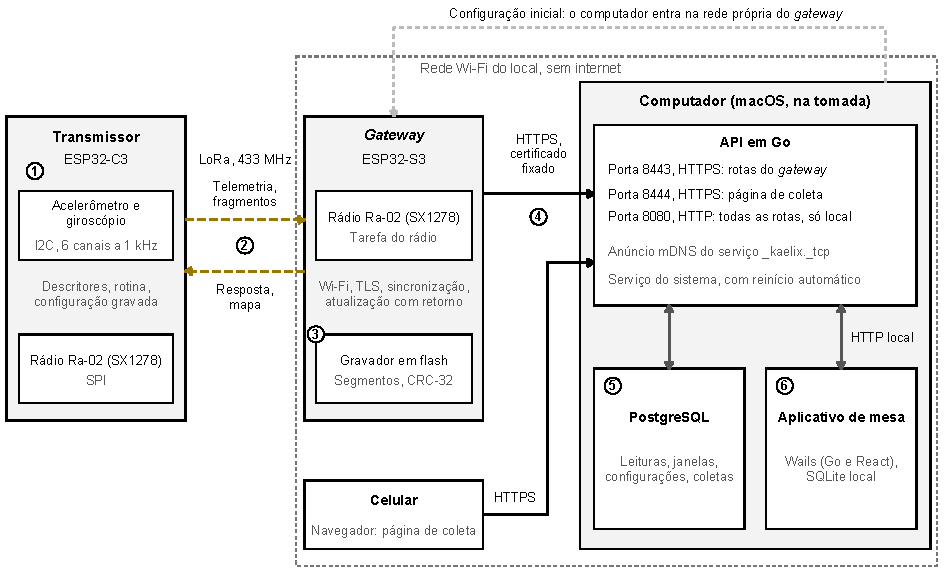
\includegraphics[width=\textwidth]{fig12_implantacao.pdf}
\fonte{elaborado pelo próprio autor.}
\legenda{os números indicam a ordem das etapas: medição no transmissor (1), envio pelo rádio (2), gravação na memória do \textit{gateway} (3), envio à API por HTTPS (4), gravação no banco (5) e consulta pelo aplicativo (6). Cada seta tem ao lado o nome do enlace. As tracejadas em amarelo-escuro são as do rádio LoRa, com a mesma cor do rádio nas Figuras~\ref{fig:sis-ciclo} e~\ref{fig:sis-configuracao}; as contínuas em preto são HTTPS pela rede Wi-Fi do local, e as em cinza, a comunicação dentro do computador.}
\end{figure}

Cada parte guarda o estado de que precisa para continuar funcionando quando a parte seguinte está fora do ar. O transmissor guarda a última configuração aceita e mede sem o \textit{gateway} (R2). O \textit{gateway} guarda as medições até a API confirmar o recebimento (R6). A API guarda a configuração desejada de cada dispositivo e a entrega ao \textit{gateway} na sincronização seguinte, a consulta que o \textit{gateway} faz à API a cada \SI{5}{\second}. O \textit{gateway}, por sua vez, repassa a configuração ao transmissor na próxima resposta pelo rádio.

O transmissor envia a janela de sinal bruto inteira, além dos indicadores (R7), e a janela ocupa o rádio por mais tempo que a telemetria. A telemetria de \num{71} bytes ocupa o rádio por \SI{411}{\milli\second}, e os \num{26} fragmentos de uma janela, por \SI{5,1}{\second}, sem contar os intervalos e os reenvios (seção~\ref{sec:fund-lora}). Com o sinal bruto no banco, a detecção pôde ser refeita com outra regra sobre as mesmas janelas, como nas análises posteriores (seção~\ref{sec:res-posteriores}).

A API atende em três portas, cada uma com um conjunto de rotas, os endereços de requisição que ela aceita. A porta \num{8080}, em HTTP, sem cifra, aceita todas as rotas, mas apenas em conexões do próprio computador, e serve ao aplicativo de mesa. A porta \num{8443}, em HTTPS, fica aberta à rede local e aceita apenas as rotas do \textit{gateway}. A porta \num{8444}, também em HTTPS, serve a página de coleta e só é aberta quando configurada.

O protocolo de rádio é definido num único arquivo de cabeçalho em C++, incluído na compilação dos dois \textit{firmwares}. Da mesma forma, a API e o aplicativo usam o mesmo pacote em Go, o pacote de contratos, para os formatos das mensagens e para as regras de validação da configuração (Quadro~\ref{quadro:sis-componentes}). Uma mudança no formato de um quadro de rádio é feita, assim, num único lugar e vale para os dois \textit{firmwares} a partir da compilação seguinte, e uma mudança numa mensagem vale para a API e para o aplicativo.

\begin{quadro}[!htb]
\centering\small
\caption{Componentes de \textit{software} do sistema}\label{quadro:sis-componentes}
\begin{tabular}{@{}>{\raggedright\arraybackslash}p{28mm}>{\raggedright\arraybackslash}p{50mm}r>{\raggedright\arraybackslash}p{46mm}@{}}
\toprule
Componente & Linguagem e bibliotecas & Linhas & Função \\
\midrule
\textit{Firmware} do transmissor & C++17 e C, Arduino-ESP32 2.0.17, RadioLib 7.7.1 & \sisLinhasTransmissor & aquisição, indicadores, telemetria, rajada, configuração e rotina \\
\addlinespace
\textit{Firmware} do \textit{gateway} & C++17, Arduino-ESP32 2.0.17, RadioLib 7.7.1, ArduinoJson 7.4.2, LittleFS & \sisLinhasGateway & recepção, gravação na \textit{flash}, entrega por HTTPS, configuração sem cabo e atualização \\
\addlinespace
Protocolo de rádio & C++17, cabeçalho único & \sisLinhasProtocolo & quadros, validação, perfis e tempos, compilado nos dois \textit{firmwares} \\
\addlinespace
Bibliotecas comuns & C++17 & \sisLinhasComum & CRC, códigos de estado e processamento de sinal \\
\addlinespace
API & Go 1.26.6, biblioteca padrão \texttt{net/http}, pgx 5.11.0 & \sisLinhasApi & ingestão idempotente, configuração, comandos, coletas e página de coleta \\
\addlinespace
Esquema do banco & SQL, PostgreSQL & \sisLinhasSql & cinco migrações numeradas \\
\addlinespace
Contratos & Go 1.26.0 & \sisLinhasContratos & formatos das mensagens e validação da configuração \\
\addlinespace
Aplicativo de mesa & Go 1.26.0 e Wails 2.13.0; React 19.3.0 e TypeScript 5.9.3 & \sisLinhasMesaGo\ e \sisLinhasMesaUi & pareamento, configuração, coletas, sinal e exportação \\
\bottomrule
\end{tabular}
\fonte{elaborado pelo próprio autor.}
\nota{linhas dos arquivos-fonte, com comentários e linhas em branco, sem os testes; no aplicativo, a primeira contagem é do processo em Go, e a segunda, da interface. SQL: linguagem de consulta estruturada.}
\end{quadro}

\section{Protocolo de rádio}\label{sec:sis-protocolo}

O protocolo de rádio da coleta, na versão 3, tem quatro tipos de quadro (Tabela~\ref{tab:sis-quadros}). Todo quadro começa pela versão e pelo tipo e termina num CRC de \num{16} bits, calculado sobre os bytes anteriores. O CRC usa o polinômio $x^{16} + x^{12} + x^{5} + 1$, do padrão CCITT, da antiga Comissão Consultiva Internacional de Telegrafia e Telefonia. Os campos de mais de um byte são gravados com o byte menos significativo primeiro, na ordem chamada \textit{little-endian}, e sem bytes de preenchimento entre os campos. O tamanho de cada estrutura em bytes é verificado na compilação, por uma asserção estática, e uma alteração acidental no formato impede a compilação. Os campos de cada quadro estão no Apêndice~\ref{ap:protocolo}.

\begin{table}[!htb]
\centering\small
\caption{Quadros do protocolo de rádio}\label{tab:sis-quadros}
\begin{tabular}{@{}>{\raggedright\arraybackslash}p{62mm}llrr@{}}
\toprule
Quadro & Destino & Canal & Bytes & Tempo no ar (ms) \\
\midrule
Telemetria & \textit{gateway} & controle & \num{71} & \num{411} \\
Resposta sem configuração & transmissor & controle & \num{22} & \num{206} \\
Resposta com configuração e seis horários de rotina & transmissor & controle & \num{75} & \num{432} \\
Fragmento completo & \textit{gateway} & rajada & \num{254} & \num{200} \\
Mapa da rajada & transmissor & rajada & \num{44} & \num{47} \\
\bottomrule
\end{tabular}
\fonte{elaborado pelo próprio autor.}
\nota{tempo no ar calculado pela Equação~\eqref{eq:fund-toa}, com o canal de controle em fator de espalhamento (SF) 9 e banda de \SI{125}{\kilo\hertz} e a rajada no perfil padrão, SF 7 e banda de \SI{250}{\kilo\hertz}. O fragmento completo leva \num{240} bytes de amostras e \num{14} bytes de cabeçalho e CRC.}
\end{table}

O enlace usa dois canais de rádio, o de controle e o da rajada. O canal de controle leva a telemetria e a resposta do \textit{gateway}, em \SI{433}{\mega\hertz}, com fator de espalhamento 9, banda de \SI{125}{\kilo\hertz}, taxa de codificação 4/5 e palavra de sincronismo \texttt{0x12}. Os parâmetros do canal de controle são constantes do \textit{firmware} e não fazem parte da configuração remota (R3). O canal da rajada leva os fragmentos da janela e o mapa da rajada, quadro em que o \textit{gateway} informa quais fragmentos recebeu. Ele usa um dos quatro perfis da Tabela~\ref{tab:sis-perfis}, escolhido na configuração do transmissor e informado na telemetria, e o \textit{gateway} passa ao perfil informado. O perfil padrão, com fator de espalhamento 7 e banda de \SI{250}{\kilo\hertz}, transmite a \SI{10,94}{kbit/s}, cerca de seis vezes a taxa do canal de controle.

\begin{table}[!htb]
\centering\small
\caption{Perfis da rajada}\label{tab:sis-perfis}
\begin{tabular}{@{}cccccc@{}}
\toprule
Código & SF & Banda (kHz) & Taxa (kbit/s) & Janela no ar (s) & Ciclo mínimo (s) \\
\midrule
0 & 9 & \num{125} & \num{1,76} & \num{32,1} & \num{36} \\
1 & 7 & \num{125} & \num{5,47} & \num{10,3} & \num{14} \\
2 (padrão) & 7 & \num{250} & \num{10,94} & \num{5,1} & \num{9} \\
3 & 7 & \num{500} & \num{21,88} & \num{2,6} & \num{7} \\
\bottomrule
\end{tabular}
\fonte{elaborado pelo próprio autor.}
\nota{SF: fator de espalhamento. Janela de \num{512} amostras em seis canais, dividida em \num{26} fragmentos. ``Janela no ar'' é a soma dos tempos no ar dos fragmentos, sem os intervalos e sem reenvios. ``Ciclo mínimo'' é o menor intervalo entre ciclos que a API aceita para essa janela, pela regra da seção~\ref{sec:sis-configuracao}.}
\end{table}

A taxa de todos os perfis fica abaixo da taxa do sinal contínuo, e por isso o transmissor envia janelas separadas por intervalos. Os seis canais a \SI{1}{\kilo\hertz}, com \num{16} bits por amostra, somam \SI{96}{kbit/s}, quase nove vezes a taxa do perfil padrão. Uma janela de \num{512} amostras dos seis canais tem \num{6144} bytes e é dividida em \num{26} fragmentos, \num{25} com \num{240} bytes de amostras e o último com \num{144}. No perfil 0, que usa os parâmetros do canal de controle, os \num{26} fragmentos ocupam o rádio por \SI{32,1}{\second}, e no perfil padrão, por \SI{5,1}{\second}. Um perfil de taxa maior ocupa o rádio por menos tempo, mas exige sinal mais forte no receptor \cite{semtech2015}. O alcance de cada perfil não foi medido.

A telemetria é enviada em todo ciclo, com ou sem janela. O número de sequência da telemetria cresce a cada ciclo, e a contagem de inicializações cresce a cada reinício do transmissor por perda de energia. Juntos, os dois números distinguem uma telemetria perdida, que deixa lacuna na sequência, de um reinício, que a faz voltar a zero (seção~\ref{sec:sis-transmissor}). Ao ligar, o transmissor não tem hora válida. A hora passa a valer quando uma resposta do \textit{gateway} a sincroniza, e um sinalizador da telemetria indica se a sincronização já ocorreu.

Num ciclo com janela, a telemetria, a resposta e os fragmentos ocupam o rádio em sequência, e a rajada só começa depois que o \textit{gateway} a autoriza (Figura~\ref{fig:sis-ciclo}). O transmissor lê a janela, o que leva \SI{512}{\milli\second} com \num{512} amostras, envia a telemetria no canal de controle e abre a recepção por até \SI{300}{\milli\second}. O \textit{gateway} responde \SI{20}{\milli\second} depois do fim da telemetria. A resposta confirma o número de sequência e leva a hora em tempo universal coordenado (UTC), a configuração desejada, quando a versão difere da relatada, e o comando pendente, quando há um. O \textit{gateway} só autoriza a rajada depois de reservar memória para a janela e conferir o número de fragmentos anunciado. Com a autorização, os dois passam ao perfil da rajada, e o transmissor envia o primeiro fragmento \SI{120}{\milli\second} depois e os seguintes com \SI{50}{\milli\second} entre eles. Os \SI{120}{\milli\second} dão ao \textit{gateway} tempo para trocar de perfil e passar a leitura à tarefa que a grava na \textit{flash} (seção~\ref{sec:sis-gravador}).

\begin{figure}[!htb]
\centering
\caption{Ciclo de medição com janela no perfil padrão da rajada}\label{fig:sis-ciclo}
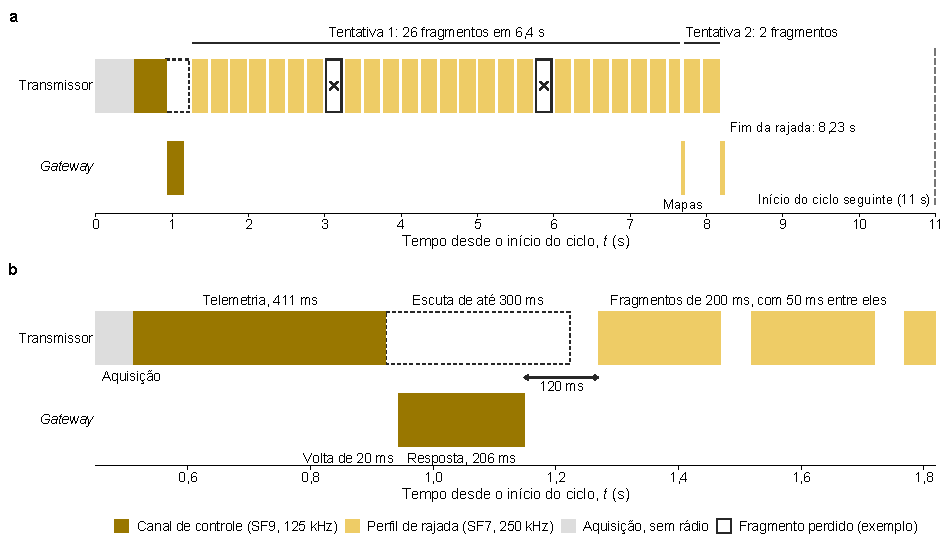
\includegraphics[width=\textwidth]{fig13_ciclo_radio.pdf}
\fonte{elaborado pelo próprio autor.}
\legenda{tempos calculados pela Equação~\eqref{eq:fund-toa}, para janela de \num{512} amostras em seis canais; os dois fragmentos perdidos são um exemplo. \textbf{a}, ciclo completo, com duas tentativas na rajada. \textbf{b}, início do ciclo: telemetria, escuta, resposta e primeiros fragmentos.}
\end{figure}

Ao fim de cada tentativa da rajada, o \textit{gateway} envia o mapa, com um bit por fragmento recebido, e o transmissor reenvia apenas os fragmentos ausentes (seção~\ref{sec:fund-blocos}). A tentativa termina depois de um silêncio de duas durações de fragmento mais \SI{100}{\milli\second}, e a rajada tem no máximo três tentativas, o envio inicial e dois reenvios. Uma janela incompleta depois da terceira tentativa é gravada com a lista dos fragmentos ausentes, e as amostras desses fragmentos chegam ao banco com valor zero. Quando nenhum fragmento chega, o \textit{gateway} não envia mapa, e o transmissor, sem o mapa, descarta a janela. No exemplo da Figura~\ref{fig:sis-ciclo}, com dois fragmentos perdidos na primeira tentativa, a rajada termina \SI{8,2}{\second} depois do início do ciclo, antes do ciclo seguinte, que começa em \SI{11}{\second}.

Um quadro corrompido no ar é descartado sem resposta. O circuito de rádio SX1278 descarta o quadro cujo CRC de rádio não confere, e o receptor confere o CRC do protocolo antes de decodificar o quadro aceito. O \textit{gateway} descarta também, sem responder, o quadro com versão ou tipo errados. Como a telemetria não é retransmitida e o \textit{gateway} só autoriza a rajada depois de recebê-la, uma telemetria perdida faz perder também a janela do ciclo. A perda fica registrada como lacuna no número de sequência.

\section{\textit{Firmware} do transmissor}\label{sec:sis-transmissor}

O transmissor usa um ESP32-C3 ligado ao módulo do acelerômetro e giroscópio pelo barramento I2C e ao rádio Ra-02, com o circuito SX1278, por uma interface serial periférica (SPI) (seção~\ref{sec:sistema}). O \textit{firmware} foi escrito em C++ com o \textit{framework} Arduino e compilado com o PlatformIO, num ambiente de compilação que inclui apenas os módulos do transmissor: o ciclo de medição, o acesso ao sensor, o acesso ao rádio, o cálculo dos indicadores e os temporizadores de vigilância (\textit{watchdog}). A imagem do \textit{firmware} da coleta, o arquivo binário gravado na placa, ocupou \sisRamTransmissorPct~\% da memória de acesso aleatório (RAM) disponível, ou \sisRamTransmissorBytes\ bytes, e \sisFlashTransmissorPct~\% do espaço de aplicação da \textit{flash}, ou \sisFlashTransmissorBytes\ de \sisFlashTransmissorTotal\ bytes. O transmissor não aloca memória dinamicamente, e a janela e os vetores de cálculo têm tamanho fixo, definido na compilação.

\subsection{Aquisição}

Na inicialização, o \textit{firmware} lê o registrador de identificação do sensor e aceita dois valores: \texttt{0x68}, do MPU-6050, e \texttt{0x74}, que ele associa ao MPU6515. A memória interna do sensor, em que o primeiro dado a entrar é o primeiro a sair (FIFO), tem \num{512} bytes no MPU6515 e \num{1024} bytes no MPU-6050. O módulo da coleta respondeu \texttt{0x74} (seção~\ref{sec:sistema}). Depois de escrever os registradores de configuração, o \textit{firmware} os lê de volta e interrompe a medição com código de erro se algum valor diferir do escrito.

O sensor amostra a \SI{1}{\kilo\hertz} e guarda as amostras na FIFO, que o \textit{firmware} esvazia pelo barramento I2C a \SI{400}{\kilo\hertz}, em lotes de até \num{10} amostras. O instante de cada amostra é dado, assim, pelo relógio do sensor, e uma pausa do processador não altera o espaçamento entre amostras enquanto a FIFO tiver espaço. Com seis canais, cada amostra ocupa \num{12} bytes, e a FIFO de \num{512} bytes comporta \num{42} amostras, ou \SI{42}{\milli\second} de sinal. Se a FIFO transbordar ou o barramento não responder, a aquisição termina com código de erro, e a janela não é enviada.

Depois da aquisição, o \textit{firmware} estima a taxa de amostragem da janela pelos carimbos de tempo da FIFO. Quando a taxa se afasta mais de \SI{2}{\percent} de \SI{1}{\kilo\hertz}, a telemetria informa o código de diagnóstico correspondente e os indicadores como não medidos, e a janela é enviada com a taxa estimada. Uma janela com amostra no limite da faixa do sensor recebe o sinalizador de saturação. A faixa do acelerômetro, a do giroscópio, o filtro interno e os canais são definidos pela configuração remota (seção~\ref{sec:sis-configuracao}).

\subsection{Ciclo, rotina e sono}

Cada ciclo começa num instante fixo, separado do início do anterior pelo intervalo da configuração, de \SI{11}{\second} por padrão. Quando a espera até o próximo ciclo passa de \SI{30}{\second}, o transmissor entra em sono profundo, com o rádio e o sensor desligados. Em esperas menores, apenas o rádio entra em modo de baixo consumo, e o processador e o sensor continuam ligados até o ciclo seguinte. Na coleta, com ciclos de \campoCicloUm\ e de \campoCicloDois~s, o transmissor não entrou em sono profundo, e o consumo não foi medido.

A rotina define até seis horários de medição, cada um com dias da semana, hora de início e hora de fim. Fora deles, o transmissor não mede e acorda a cada intervalo de consulta, de \SI{300}{\second} por padrão, para enviar uma telemetria sem medição, marcada por um sinalizador, e receber comandos. A rotina só é seguida depois que o transmissor recebe a hora do \textit{gateway}, e, sem hora sincronizada, ele mede em todos os ciclos.

Dois temporizadores de vigilância reiniciam o transmissor quando o ciclo para. O da tarefa tem prazo de \SI{6}{\second}, e o ligado ao relógio de tempo real (RTC) tem prazo de \SI{20}{\second} por ciclo, estendido durante a rajada.

A telemetria seguinte a um reinício permite saber se ele foi causado por perda de energia. O número de sequência fica na memória do RTC, que se mantém no sono profundo e num reinício por \textit{software} e se perde quando a alimentação é interrompida. Depois de uma interrupção, o estado guardado no RTC não passa na conferência do CRC, o número de sequência volta a zero e a contagem de inicializações, guardada na memória não volátil, cresce. A telemetria informa também a causa do último reinício, registrada pelo próprio ESP32-C3. Pelo número de sequência, pela contagem de inicializações e pela causa do reinício, foram identificados na coleta os reinícios por queda de tensão da bateria (seção~\ref{sec:res-aquisicao}).

\subsection{Indicadores e diagnóstico}

A cada janela, o transmissor calcula o valor eficaz nos três eixos de aceleração. No eixo Z, depois de remover a média da janela, calcula também a curtose, o fator de crista e a frequência dominante, o pico do espectro da velocidade entre \SI{10}{\hertz} e a metade da taxa de amostragem. A telemetria leva ainda a taxa de amostragem estimada e a temperatura interna do sensor. As funções de cálculo ficam numa biblioteca separada do acesso ao \textit{hardware} e são testadas no computador (seção~\ref{sec:sis-testes}). Os indicadores do transmissor não foram usados na avaliação da detecção, que usou os descritores calculados sobre as janelas exportadas (seção~\ref{sec:descritores}). Um detector Isolation Forest de \num{100} árvores, treinado em Python para o \textit{firmware} de bancada, foi convertido em código C++, mas esse código não entra na compilação do transmissor da coleta.

Cada função do \textit{firmware} devolve um código de estado, e o campo de diagnóstico da telemetria informa o primeiro erro do ciclo (Quadro~\ref{quadro:sis-diagnostico}). Quando a aquisição não se completa, os indicadores são enviados como valor não numérico (NaN), e a telemetria do ciclo é transmitida normalmente. Uma versão anterior do \textit{firmware} preenchia a janela com zeros em caso de erro, e os indicadores calculados sobre esses zeros seriam classificados como máquina sadia. O código de diagnóstico foi zero em \sisCampoDiagZero\ das \sisCampoTelemetrias\ telemetrias dos trechos analisados.

\begin{quadro}[!htb]
\centering\small
\caption{Códigos de diagnóstico da telemetria}\label{quadro:sis-diagnostico}
\begin{tabular}{@{}l>{\raggedright\arraybackslash}p{68mm}>{\raggedright\arraybackslash}p{60mm}@{}}
\toprule
Código & Condição & Efeito no ciclo \\
\midrule
\texttt{0x10} & sensor ausente no barramento & indicadores como NaN; sem janela \\
\texttt{0x11} & identificação diferente de \texttt{0x68} e de \texttt{0x74} & indicadores como NaN; sem janela \\
\texttt{0x15} & FIFO transbordada ou taxa estimada a mais de \SI{2}{\percent} de \SI{1}{\kilo\hertz} & sem janela, no primeiro caso; indicadores como NaN, no segundo \\
\texttt{0x16} & amostra em $\pm\num{32760}$, no limite da faixa & sinalizador de saturação; janela enviada \\
\texttt{0x17} & janela com valor constante & indicadores como NaN; janela enviada \\
\bottomrule
\end{tabular}
\fonte{elaborado pelo próprio autor.}
\nota{os erros de barramento (tempo-limite e ausência de resposta) têm códigos próprios e terminam a aquisição como no primeiro caso.}
\end{quadro}

\section{\textit{Firmware} do \textit{gateway}}\label{sec:sis-gateway}

O \textit{gateway} usa um ESP32-S3 com \SI{16}{MiB} de memória \textit{flash} e \SI{8}{MiB} de memória pseudoestática (PSRAM), ligado ao mesmo modelo de rádio do transmissor. Ele recebe as telemetrias e as janelas pelo rádio, grava as medições, entrega os dados à API e repassa ao transmissor a configuração e os comandos. A imagem da coleta, na versão 2.1.1, ocupou \sisRamGatewayPct~\% da RAM, ou \sisRamGatewayBytes\ bytes, e \sisFlashGatewayPct~\% do espaço de aplicação, ou \sisFlashGatewayBytes\ de \sisFlashGatewayTotal\ bytes.

\subsection{Tarefas e gravador}\label{sec:sis-gravador}

O trabalho do \textit{gateway} é dividido em três contextos de execução do FreeRTOS, o sistema operacional de tempo real incluído no \textit{framework} Arduino do ESP32. O laço principal atende o rádio e é o único a usar o barramento SPI, uma tarefa grava os registros na \textit{flash}, e outra, de prioridade menor, cuida da rede. O laço do rádio responde ao transmissor antes de gravar a telemetria e passa cada leitura e cada janela à tarefa de gravação por uma fila de \num{32} posições. Com essa divisão, um envio lento à API não atrasa a resposta pelo rádio, enviada \SI{20}{\milli\second} depois do fim da telemetria. Com a fila cheia, o registro é contado como descartado, e o número de descartes é informado na mensagem periódica de estado (\textit{heartbeat}) que o \textit{gateway} envia à API. A cada \SI{5}{\second}, o laço do rádio lê o registrador de versão do SX1278 para conferir que o rádio responde, e um temporizador de vigilância reinicia o \textit{gateway} se uma tarefa parar.

O gravador é a parte do \textit{firmware} que guarda as medições na \textit{flash} até a confirmação da API. Ele usa uma partição de \SI{9,88}{MiB}, formatada com o sistema de arquivos LittleFS (Figura~\ref{fig:sis-atualizacao}a), e escreve em segmentos de \SI{256}{KiB}. Cada registro tem um cabeçalho de \num{12} bytes, com tipo, tamanho e CRC de \num{32} bits, e passa a valer apenas depois de gravado e sincronizado com a \textit{flash}. Cada inicialização abre um segmento novo, e por isso um registro cortado por queda de energia só pode estar no fim de um segmento antigo. Ao encontrar, num segmento antigo, um registro incompleto ou com CRC errado, a tarefa de rede o conta como corrompido e passa a ler o segmento seguinte. Quando a escrita de um registro retorna erro, a tarefa de gravação tenta de novo até três vezes, e um registro não gravado é contado como descartado. A posição do último registro confirmado pela API também é gravada com CRC, a cada \num{16} confirmações.

O gravador comporta \num{1442} ciclos com janela padrão, o que corresponde a \SI{4,4}{\hour} de coleta com intervalo de \SI{11}{\second} e janela em todo ciclo. Cada ciclo ocupa \num{6460} bytes, \num{143} da leitura e \num{6317} da janela, com os cabeçalhos, e o gravador usa até \SI{90}{\percent} do sistema de arquivos. Com o gravador cheio, o segmento mais antigo é apagado, e o número de registros descartados é informado na mensagem de estado. A retenção do requisito R6 vale, portanto, dentro dessa capacidade.

A tarefa de rede lê o gravador a partir da última posição confirmada e envia à API as leituras em lotes de até oito e cada janela numa requisição própria. Cada leitura e cada janela leva o identificador do \textit{gateway}, o da sessão de inicialização, sorteado a cada inicialização, e um número de ordem crescente, atribuído pelo \textit{gateway}. A API grava cada registro uma única vez por esse trio, e por isso um reenvio depois de uma queda da rede ou da API não duplica dados (seção~\ref{sec:fund-entrega}). A tarefa só avança a posição confirmada quando a resposta da API indica cada registro enviado como gravado ou repetido. Quando a resposta indica erro permanente, como corpo inválido ou conflito de conteúdo, a tarefa descarta o registro. Nos demais erros, a tarefa repete o envio com espera crescente, de \SIrange{1}{30}{\second}, e, depois de três erros seguidos, procura a API de novo na rede.

O \textit{gateway} mantém também um histórico de eventos, uma sequência de linhas de texto que descrevem a sua operação, como a recepção de cada rajada. A memória do \textit{gateway} guarda até \num{64} linhas, que são enviadas à API, e a API mantém as \num{5000} linhas mais recentes de cada \textit{gateway}. A linha de cada rajada informa o número de fragmentos recebidos e a duração, e as rajadas analisadas na seção~\ref{sec:res-aquisicao} foram extraídas desse histórico (seção~\ref{sec:dados}).

\subsection{Rede e segurança}

O \textit{gateway} guarda até cinco redes Wi-Fi e conecta-se à de sinal mais forte. Ele localiza a API pelo anúncio que ela faz na rede local por resolução de nomes por difusão (mDNS), sem endereço de protocolo de internet (IP) gravado. Por isso, uma mudança no endereço do computador não exige regravar o \textit{gateway}.

A conexão com a API usa TLS, com um certificado próprio, gerado pela API na primeira execução, sem autoridade certificadora (seção~\ref{sec:fund-tls}). O \textit{gateway} compara o resumo SHA-256 do certificado recebido com o resumo gravado na configuração inicial e, se os dois diferirem, encerra a conexão antes de enviar a credencial (R8). A credencial é uma sequência aleatória de \num{43} caracteres (\textit{token}), enviada em cada requisição, e a API guarda apenas o resumo SHA-256 dela.

Sem rede conhecida por \SI{30}{\second}, o \textit{gateway} abre uma rede Wi-Fi própria, com nome formado pelos últimos quatro dígitos do endereço de controle de acesso ao meio (MAC), e oferece quatro rotas HTTP locais: informações do \textit{gateway}, lista das redes visíveis, configuração inicial e reinício. O assistente do aplicativo usa essa rede para enviar ao \textit{gateway} o identificador, o \textit{token}, uma chave de administração, o resumo do certificado e as redes Wi-Fi do local. Enquanto a rede própria está aberta, o \textit{gateway} continua a receber e a gravar as medições do rádio. Manter pressionado o botão de inicialização por \SI{10}{\second} apaga o pareamento, isto é, os dados recebidos na configuração inicial.

\subsection{Atualização sem cabo}

A \textit{flash} tem dois espaços de aplicação de \SI{3}{MiB}, e a imagem nova é gravada no espaço que não está em uso, sem apagar a que está em execução (Figura~\ref{fig:sis-atualizacao}a). O aplicativo envia a imagem à API, e a sincronização seguinte informa ao \textit{gateway} a versão, o tamanho, o resumo SHA-256 e o endereço de onde baixá-la. O \textit{gateway} baixa a imagem por HTTPS, confere o tamanho e o resumo e reinicia com ela. Uma imagem com tamanho ou resumo diferente é descartada, e o \textit{gateway} continua na versão atual.

\begin{figure}[!htb]
\centering
\caption{Partições da \textit{flash} do \textit{gateway} e etapas da atualização sem cabo}\label{fig:sis-atualizacao}
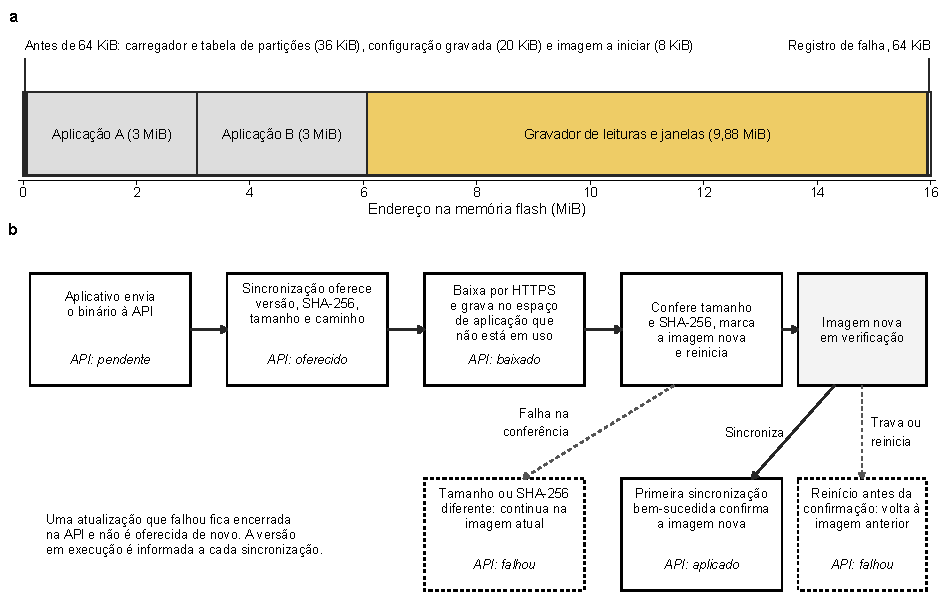
\includegraphics[width=\textwidth]{fig15_atualizacao.pdf}
\fonte{elaborado pelo próprio autor.}
\legenda{\textbf{a}, partições definidas na tabela do \textit{firmware}, em escala. \textbf{b}, etapas da atualização, com o estado registrado pela API em cada uma; as caixas tracejadas são as saídas sem sucesso.}
\end{figure}

A imagem nova fica em verificação até a primeira sincronização bem-sucedida com a API, que a confirma. Se o \textit{gateway} reiniciar antes da confirmação, o carregador de inicialização volta à imagem anterior, e a API registra a atualização como malsucedida (R9). Uma atualização malsucedida fica encerrada na API e não é oferecida de novo. A atualização sem cabo cobre apenas o \textit{gateway}, e o \textit{firmware} do transmissor é gravado pela porta de barramento serial universal (USB).

\section{Configuração remota e comandos}\label{sec:sis-configuracao}

A configuração do transmissor tem \num{14} campos (Quadro~\ref{quadro:sis-config}), e cada alteração recebe da API um número de versão. As faixas de cada campo e a regra do ciclo mínimo ficam no pacote de contratos, usado pela API e pelo aplicativo, e os dois recusam a mesma configuração pelo mesmo motivo. Pela regra do ciclo mínimo, a soma do tempo de aquisição, do tempo do canal de controle e do tempo da rajada, calculado pela Equação~\eqref{eq:fund-toa}, não pode ultrapassar o intervalo do ciclo. A configuração que o ultrapassa é recusada com a indicação do intervalo mínimo.

\begin{quadro}[!htb]
\centering\small
\caption{Campos da configuração do transmissor}\label{quadro:sis-config}
\begin{tabular}{@{}>{\raggedright\arraybackslash}p{50mm}>{\raggedright\arraybackslash}p{56mm}>{\raggedright\arraybackslash}p{44mm}@{}}
\toprule
Campo & Valores aceitos & Padrão \\
\midrule
Intervalo do ciclo & \SIrange{1}{3600}{\second} & \SI{11}{\second} \\
Amostras por canal & \num{256} a \num{4096}, em potências de 2 & \num{512} \\
Canais & combinação dos seis, com o eixo Z & os seis \\
Faixa do acelerômetro & $\pm\SI{2}{g}$ a $\pm\SI{16}{g}$ & $\pm\SI{4}{g}$ \\
Faixa do giroscópio & $\pm\SI{250}{\degree\per\second}$ a $\pm\SI{2000}{\degree\per\second}$ & $\pm\SI{250}{\degree\per\second}$ \\
Filtro interno do sensor & códigos 0 a 6 & 1, banda de \SI{184}{\hertz} \\
Potência de transmissão & \SIrange{2}{17}{dBm} & \SI{10}{dBm} \\
Perfil da rajada & 0 a 3 (Tabela~\ref{tab:sis-perfis}) & 2 \\
Janela a cada $N$ ciclos & 0 a \num{255}; 0 desliga o sinal bruto & 1 \\
Prazo de perda do enlace & \SIrange{60}{86400}{\second} & \SI{900}{\second} \\
Intervalo de consulta fora da rotina & \SIrange{60}{3600}{\second} & \SI{300}{\second} \\
Fuso horário da rotina & \SIrange{-720}{840}{\minute} & \SI{-180}{\minute} \\
Rotina & até seis horários de medição, com dias e horas & vazia, sempre ligado \\
Versão & \num{1} a \num{65535}, atribuída pela API & 0, configuração de fábrica \\
\bottomrule
\end{tabular}
\fonte{elaborado pelo próprio autor.}
\end{quadro}

Uma configuração nova passa por três estados na API, pendente, enviada e aplicada, e só é marcada como aplicada quando a telemetria do transmissor informa a versão nova (Figura~\ref{fig:sis-configuracao}). O aplicativo grava a configuração na API, que lhe atribui uma versão e a marca como pendente. A cada sincronização, o \textit{gateway} recebe da API as configurações e os comandos ainda não confirmados e os guarda numa tabela de até oito transmissores, na memória não volátil. Na telemetria seguinte daquele transmissor, a resposta leva a configuração, e a sincronização seguinte informa à API que ela foi enviada pelo rádio. O \textit{gateway} repete a configuração em cada resposta enquanto a versão relatada na telemetria for outra. A API marca a configuração como aplicada quando grava uma leitura com a versão nova (R4).

\begin{figure}[!htb]
\centering
\caption{Sequência de uma configuração nova do transmissor}\label{fig:sis-configuracao}
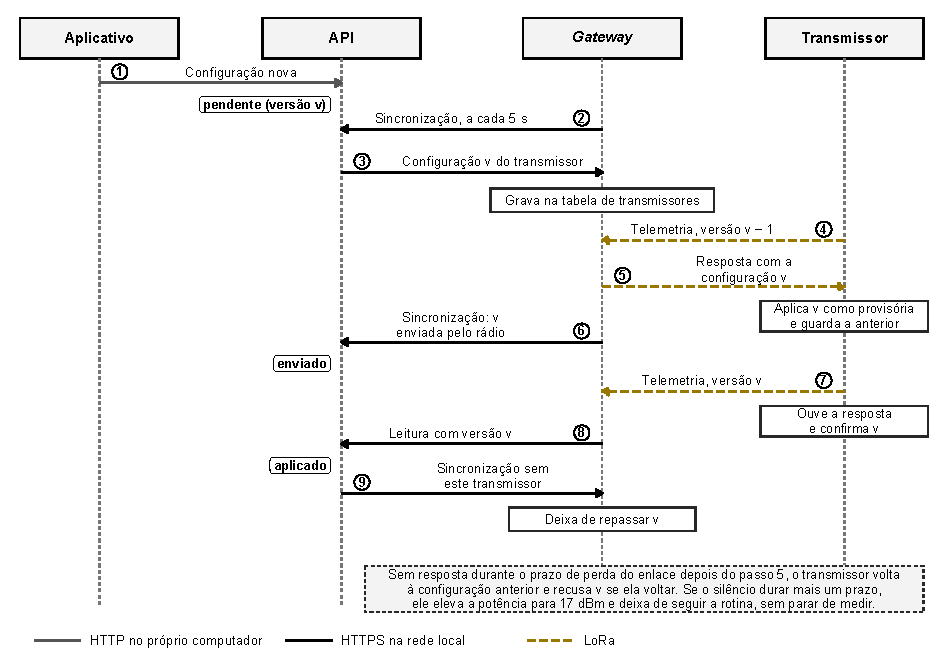
\includegraphics[width=\textwidth]{fig14_configuracao.pdf}
\fonte{elaborado pelo próprio autor.}
\legenda{os números indicam a ordem das mensagens, e os rótulos em negrito são os estados que a API registra para a configuração. $v$: versão da configuração nova.}
\end{figure}

O transmissor aplica a configuração nova como provisória e guarda a anterior na memória não volátil. Se não ouvir o \textit{gateway} durante o prazo de perda do enlace, de \SI{900}{\second} por padrão, ele volta à configuração anterior, que recebe um prazo novo, e recusa a versão revertida se ela for oferecida de novo (R5). Quando o prazo se esgota sem configuração provisória, o transmissor eleva a potência para \SI{17}{dBm} e deixa de seguir a rotina, sem parar de medir. Ao ouvir o \textit{gateway} de novo, ele volta à potência e à rotina da configuração.

O aplicativo envia ao transmissor três comandos, o de reinício, o de restauração da configuração de fábrica e o de captura de uma janela fora da rotina. Cada comando recebe um número crescente por transmissor, e a telemetria devolve o número do último comando executado. Ao registrar uma restauração de fábrica, a API troca também a configuração desejada pelos valores padrão, com versão nova, para que a configuração antiga não volte na sincronização seguinte.

O \textit{gateway} tem configuração própria, com as redes Wi-Fi, o intervalo da mensagem de estado (\SI{30}{\second}), o intervalo da sincronização (\SI{5}{\second}), a opção de abrir a rede própria quando nenhuma rede conhecida está ao alcance e a potência da resposta pelo rádio (\SI{17}{dBm}). As senhas de Wi-Fi ficam cifradas no banco e são enviadas ao \textit{gateway} apenas quando a versão da configuração do \textit{gateway} muda.

\section{API, banco de dados e aplicativo}\label{sec:sis-api}

A API foi escrita em Go, com a biblioteca padrão para o HTTP, e grava os dados em PostgreSQL. No computador da coleta, ela é executada como serviço do sistema operacional, que a reinicia se o processo terminar. O esquema do banco tem \num{16} tabelas (Quadro~\ref{quadro:sis-banco}), criadas por cinco migrações, alterações do esquema numeradas em ordem e aplicadas numa única transação. A tabela de leituras guarda a telemetria inteira, e a de janelas guarda o sinal bruto, como inteiros de \num{16} bits intercalados por canal, com a lista de fragmentos ausentes. A API não apaga leituras, janelas nem coletas.

\begin{quadro}[!htb]
\centering\small
\caption{Tabelas do banco de dados da API}\label{quadro:sis-banco}
\begin{tabular}{@{}>{\raggedright\arraybackslash}p{36mm}c>{\raggedright\arraybackslash}p{96mm}@{}}
\toprule
Grupo & Tabelas & Conteúdo \\
\midrule
Usuários & 2 & contas e sessões de usuário do aplicativo \\
\addlinespace
\textit{Gateways} & 7 & cadastro, sessões de inicialização, mensagens de estado, histórico de eventos, configuração e atualizações \\
\addlinespace
Transmissores e máquinas & 4 & cadastro dos transmissores e das máquinas, configuração desejada e relatada, comandos \\
\addlinespace
Medições & 2 & leituras e janelas de sinal bruto \\
\addlinespace
Coletas & 1 & intervalos de coleta com nome e condição da máquina \\
\bottomrule
\end{tabular}
\fonte{elaborado pelo próprio autor.}
\nota{uma das tabelas dos \textit{gateways} guarda as mensagens de estado no formato anterior ao atual.}
\end{quadro}

As rotas da API se dividem pelo cliente, o \textit{gateway} ou o aplicativo. As rotas do \textit{gateway} exigem o \textit{token} do próprio \textit{gateway}, e o identificador informado no corpo da requisição tem de coincidir com o da credencial. Elas recebem leituras, janelas, mensagens de estado e o histórico de eventos, atendem à sincronização e entregam a imagem de \textit{firmware}. As rotas do aplicativo exigem sessão de usuário e cobrem a configuração, os comandos, as janelas, as coletas, o envio de \textit{firmware} e o resumo do certificado, usado na configuração inicial do \textit{gateway}. A senha de cada usuário é guardada pela função bcrypt, própria para o resumo de senhas, e cada endereço IP tem no máximo dez tentativas de entrada por minuto.

A gravação de leituras e de janelas é idempotente, isto é, um reenvio não cria registro novo. A tabela de leituras e a de janelas têm restrição de unicidade sobre o trio formado pelo \textit{gateway}, pela sessão de inicialização e pelo número de ordem. Um lote repetido recebe a mesma confirmação, com o estado de repetido, e não gera linha nova. Um registro com o mesmo trio e conteúdo diferente é recusado como conflito, e o lote inteiro é desfeito.

Antes de gravar, a API confere o formato de cada requisição. Ela recusa o corpo com campo desconhecido ou chave repetida, o lote com mais de oito leituras e a janela cujo tamanho difere do produto do número de amostras pelo número de canais e por dois bytes. O corpo de uma janela é limitado a \SI{128}{KiB}. Ao gravar uma janela, a API calcula o resumo SHA-256 das amostras e o guarda com ela. Com esse resumo, calculado depois da recepção, é possível conferir a cópia das amostras do banco para os dados exportados (seção~\ref{sec:dados}), mas não a transmissão pelo rádio, conferida pelo CRC de cada fragmento.

As senhas de Wi-Fi são cifradas pelo padrão de cifra avançada (AES) no modo de contador com autenticação de Galois (GCM), com chave de \num{256} bits guardada num arquivo que apenas o usuário do serviço pode ler (seção~\ref{sec:fund-tls}). A chave e o certificado TLS, com chave de curva elíptica P-256, são gerados na primeira execução da API.

O aplicativo de mesa foi feito com Wails, que une um processo em Go a uma interface em React e TypeScript, e se comunica com a API pela porta local. A interface tem nove telas: monitoramento, motores, \textit{gateways}, transmissores, coletas, sinal, eventos, configurações e painel geral (Apêndice~\ref{ap:telas}). Por elas, o operador pareia e acompanha o \textit{gateway}, edita a configuração e a rotina do transmissor, envia comandos, inicia e encerra coletas e vê o resumo das perdas e o sinal de cada janela. A exportação de uma coleta gera tabelas em valores separados por vírgula (CSV), uma para as leituras, uma para a lista de janelas e uma para cada janela, com as amostras em unidades físicas e nos valores brutos do sensor. Os dados analisados neste trabalho não passaram por essa exportação. Eles foram lidos do banco em modo somente leitura por outro programa, e o resumo de cada janela foi conferido nessa leitura (seção~\ref{sec:dados}).

A página de coleta, servida pela API e aberta no celular, permite operar a coleta sem voltar ao computador (Figura~\ref{fig:sis-pagina-coleta}). Ela fica embutida no programa da API e exige a mesma conta do aplicativo. Pela página, o operador inicia e encerra coletas, muda o intervalo do ciclo do transmissor e acompanha o estado do \textit{gateway} e do transmissor e as últimas leituras, atualizadas a cada \SI{5}{\second}. Durante uma coleta, a página mostra também a duração, o número de leituras recebidas e perdidas, o número de janelas completas e a RSSI média e a menor RSSI do período.

\begin{figure}[!htb]
\centering
\caption{Página de coleta no celular, durante a coleta em campo}\label{fig:sis-pagina-coleta}
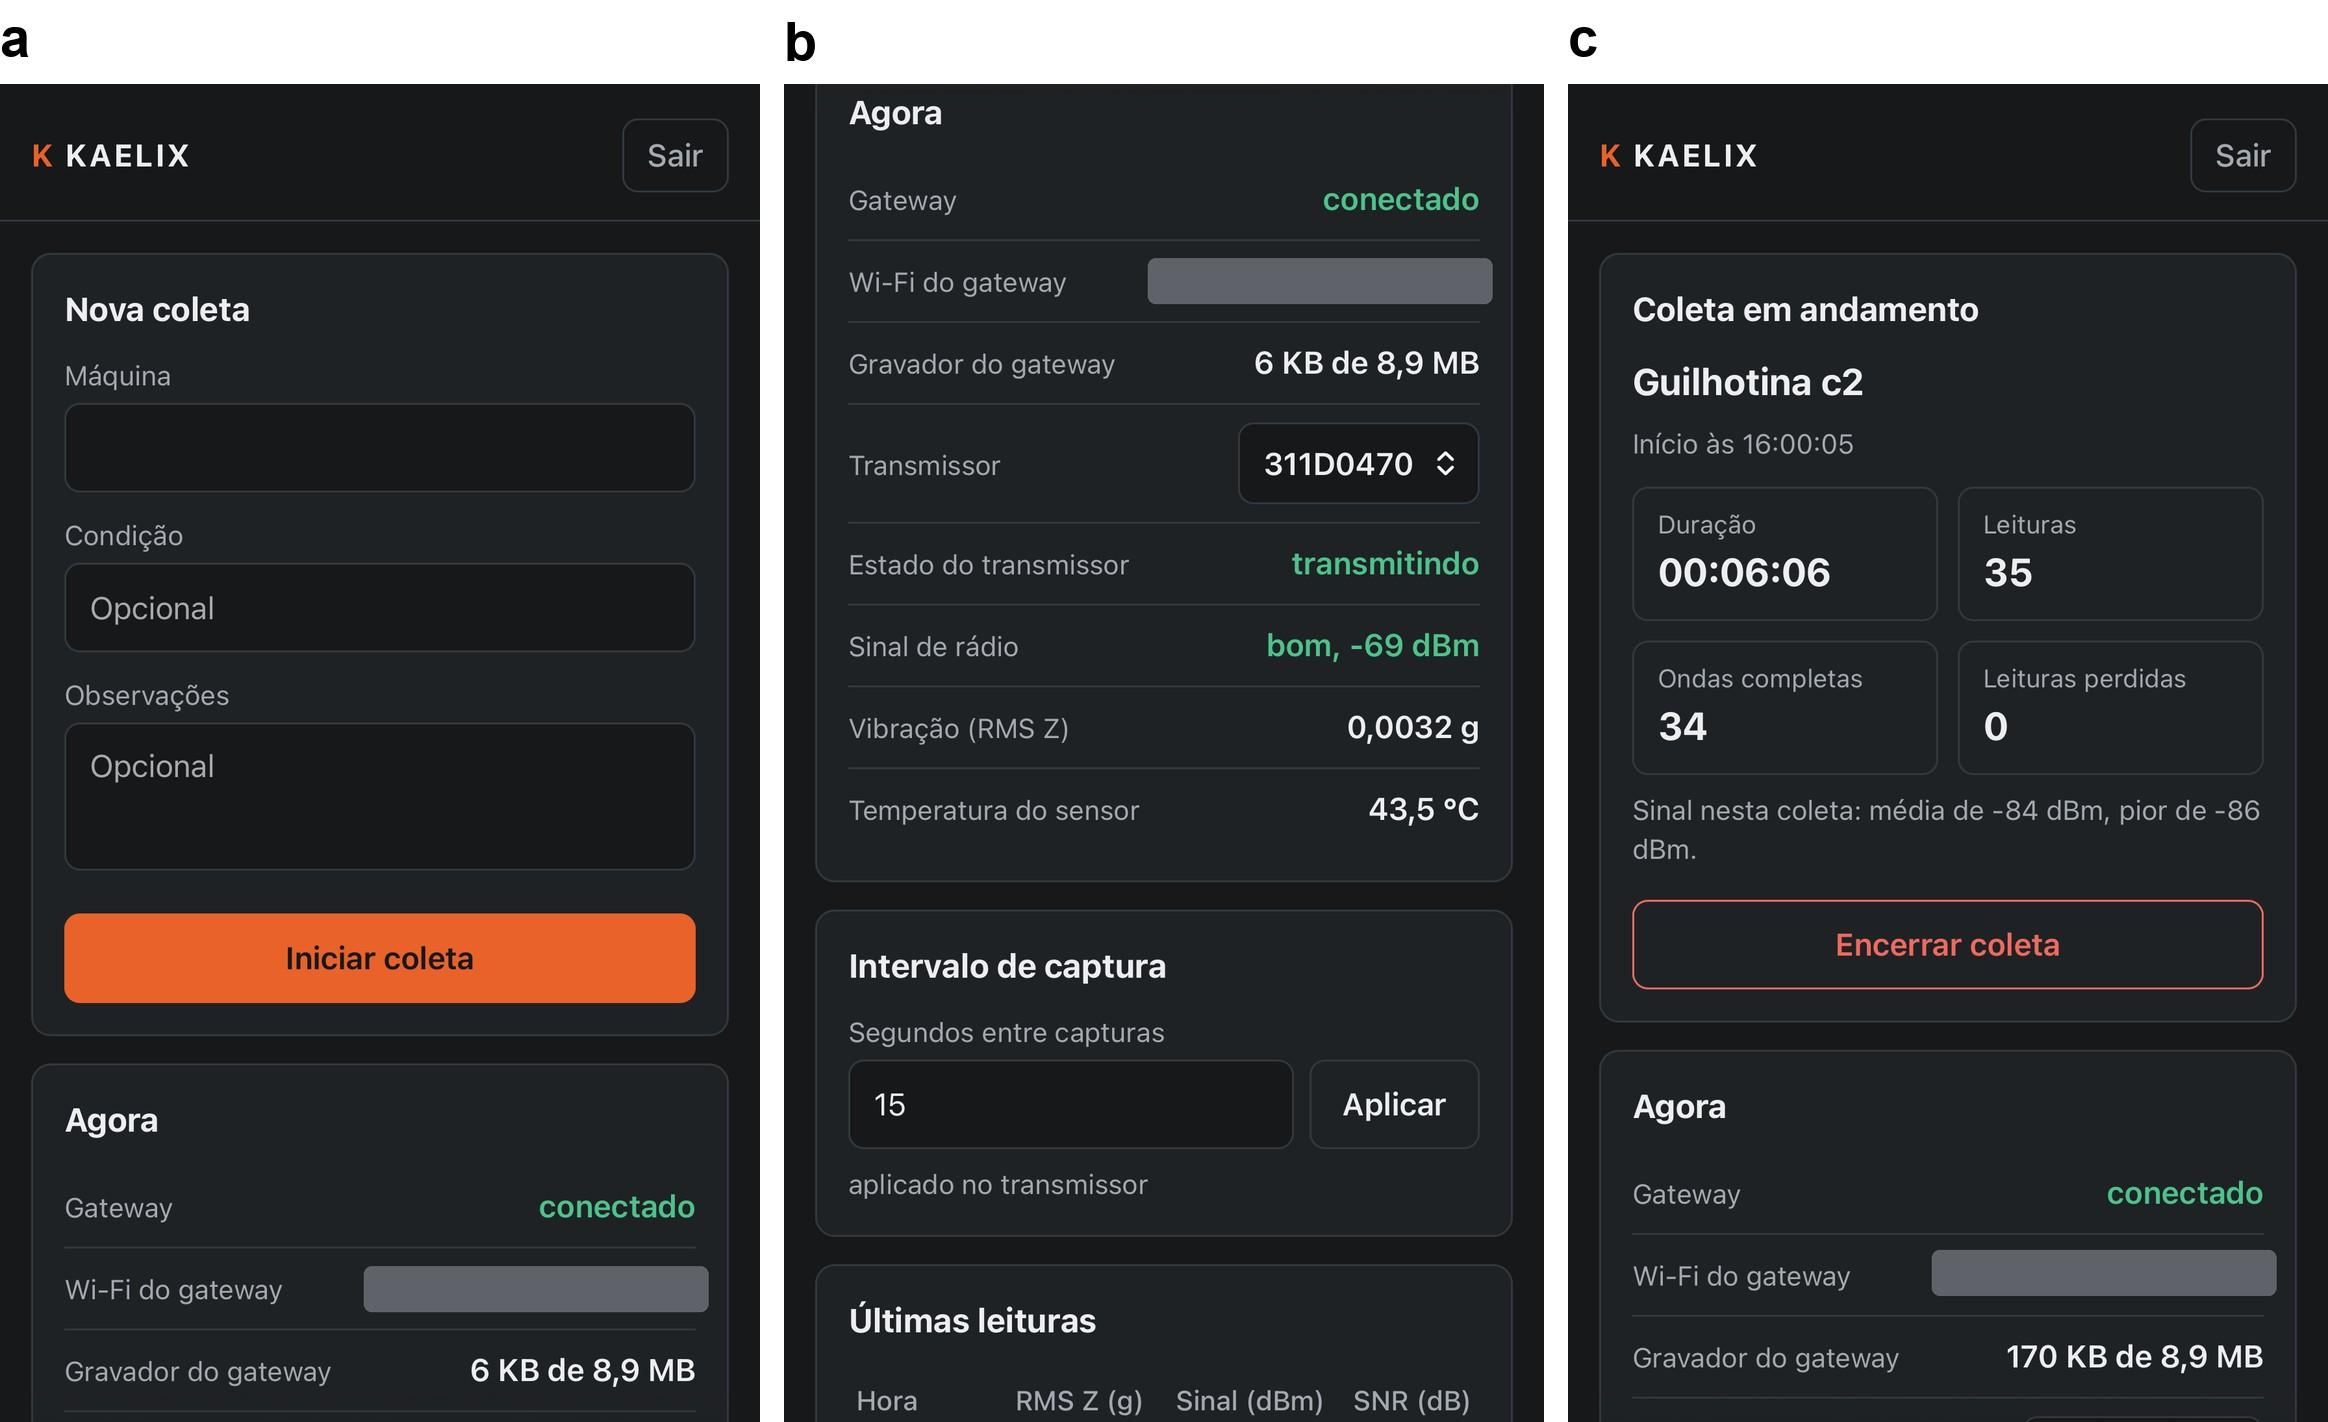
\includegraphics[width=\textwidth]{campo/fig17_pagina_coleta.jpg}
\fonte{elaborado pelo próprio autor.}
\legenda{\textbf{a}, início de uma coleta e estado do \textit{gateway}. \textbf{b}, estado do transmissor, intervalo do ciclo, chamado de intervalo de captura na página, e últimas leituras. \textbf{c}, segunda rodada da guilhotina em andamento; a captura de tela foi feita antes da chegada da última janela da rodada, e por isso a página mostra 34 ondas completas para 35 leituras. ``Ondas completas'' é o número de janelas de sinal bruto recebidas inteiras. Capturas de tela de 2 de novembro de 2026, sem a barra do navegador; o nome da rede Wi-Fi do local foi coberto por um retângulo cinza.}
\end{figure}

\section{Verificação}\label{sec:sis-verificacao}

O sistema foi verificado por quatro meios: uma norma de codificação, uma análise de modos de falha, testes automatizados no computador e ensaios de ponta a ponta no \textit{hardware} (seção~\ref{sec:fund-verificacao}). A norma e a análise de modos de falha foram escritas para o \textit{firmware} de bancada, versão anterior em que o transmissor enviava apenas os indicadores, sem a janela de sinal bruto. Os testes e os ensaios cobrem a versão da coleta.

\subsection{Norma de codificação}\label{sec:sis-norma}

O \textit{firmware} foi escrito segundo uma norma de codificação própria, com \num{41} regras em \num{14} áreas (Tabela~\ref{tab:sis-norma}). As regras foram selecionadas da MISRA C++:2008 \cite{misra2008}, que tem \num{228} regras, do padrão de codificação em C++ do programa Joint Strike Fighter \cite{jsf2005}, que tem \num{221}, e das dez regras de \citeonline{holzmann2006} para código crítico. Uma regra entrou na norma quando foi possível dizer qual falha do dispositivo ela impede e como a sua violação é detectada: pelo compilador, por análise estática, por teste ou por revisão. A norma lista \num{14} desvios aceitos, cada um com a justificativa.

\begin{table}[!htb]
\centering\small
\caption{Áreas da norma de codificação}\label{tab:sis-norma}
\begin{tabular}{@{}llc@{}}
\toprule
Prefixo & Assunto & Regras \\
\midrule
NC-ARQ & dependência entre camadas & 4 \\
NC-MEM & política de memória & 3 \\
NC-FLX & fluxo de controle: laços, recursão e limites & 4 \\
NC-ERR & tratamento e propagação de erro & 5 \\
NC-CTR & validação de parâmetros e contratos & 3 \\
NC-INI & inicialização de variáveis & 2 \\
NC-CNV & tipos e conversões & 3 \\
NC-FPU & ponto flutuante & 4 \\
NC-CST & constantes e uso de \texttt{const} & 2 \\
NC-ESC & escopo e visibilidade & 2 \\
NC-NOM & nomes & 3 \\
NC-HDR & arquivos de cabeçalho e inclusão & 2 \\
NC-COM & comentários & 2 \\
NC-BLD & compilação e verificação & 2 \\
\midrule
Total & & 41 \\
\bottomrule
\end{tabular}
\fonte{elaborado pelo próprio autor.}
\end{table}

Segundo a própria norma, as \num{41} regras servem ao requisito de que o dispositivo nunca afirme o que não mediu. As regras de tratamento de erro aplicam esse requisito diretamente: o valor não medido é NaN, nunca zero; todo caminho de erro produz o estado desconhecido; e uma função que termina com erro não escreve no seu parâmetro de saída.

A norma também proíbe alocação dinâmica de memória e recursão e exige que todo laço tenha um limite conhecido antes de começar. Com essas restrições, o tempo e a memória de cada ciclo podem ser calculados antes da execução.

Cada regra tem um meio de verificação atribuído. O compilador detecta o retorno de função não consumido, a conversão com perda de informação e a igualdade entre números de ponto flutuante, e asserções estáticas verificam na compilação o dimensionamento dos vetores e o formato dos quadros. Os testes no computador verificam as guardas de contrato, as verificações de pré-condição no início das funções. A revisão humana cobre o argumento do limite de cada laço e a classificação dos erros. O repositório do \textit{firmware} tem um \textit{script} que executa as ferramentas de análise estática clang-tidy e cppcheck para as regras de conversão, de nomes e de alocação. Não há registro de execução desse \textit{script}, e as duas ferramentas não estavam instaladas no computador de desenvolvimento em 7 de novembro de 2026.

A conformidade da versão da coleta com a norma tem três limites conhecidos. A regra NC-BLD-01 exige compilação com todos os avisos ativados e tratados como erro, e nenhum ambiente do PlatformIO, ferramenta que compila o \textit{firmware} das placas e executa os testes, ativa essas opções. A norma foi escrita em setembro de 2026 para o \textit{firmware} de bancada, antes do transmissor e do \textit{gateway} da coleta. O transmissor não aloca memória dinamicamente, mas o \textit{gateway} aloca, na fila de gravação, no gerenciador de redes Wi-Fi e na reserva da janela recebida, contra a regra NC-MEM-01, e esse uso não consta da lista de desvios.

\subsection{Análise de modos de falha}\label{sec:sis-falhas}

A análise de modos de falha e efeitos (FMEA) do \textit{firmware} de bancada listou \num{36} modos de falha em sete grupos: aquisição, temperatura, rádio, energia, execução, sono e telemetria. Cada modo recebeu uma classe de severidade, de S0 a S3, e uma classe de detectabilidade: D-A, quando o dispositivo detecta e informa a falha; D-B, quando o receptor consegue inferi-la com os dados que já recebe; e D-C, quando nenhum dos dois consegue detectá-la (seção~\ref{sec:fund-fmea}). A classe S3 é a do dado inválido aceito como válido, porque ele leva a uma decisão de manutenção errada sem nenhum sinal de erro. O Quadro~\ref{quadro:sis-falhas} mostra o mecanismo de detecção, na versão da coleta, de cada modo que continua aplicável à montagem sem termistor, sem medição de tensão da bateria e sem detector embarcado.

\begin{quadro}[!htb]
\centering\small
\caption{Modos de falha da FMEA na versão da coleta}\label{quadro:sis-falhas}
\begin{tabular}{@{}>{\raggedright\arraybackslash}p{44mm}>{\raggedright\arraybackslash}p{72mm}>{\raggedright\arraybackslash}p{34mm}@{}}
\toprule
Modo de falha & Mecanismo na versão da coleta & Quem detecta \\
\midrule
Sensor ausente ou que para no meio da janela (FM-01, FM-02) & tempo-limite ao ler a FIFO, código de erro no diagnóstico e indicadores como NaN & transmissor \\
\addlinespace
Valor saturado ou constante (FM-04) & sinalizador de saturação; código de sensor congelado para a janela constante & transmissor \\
\addlinespace
Sensor solto da máquina (FM-05) & nenhum & ninguém \\
\addlinespace
Telemetria perdida no ar (FM-11) & lacuna no número de sequência & API e operador \\
\addlinespace
Quadro corrompido (FM-13) & CRC do rádio e CRC do protocolo & \textit{gateway}, que descarta \\
\addlinespace
Queda de tensão (FM-15) & causa do reinício na telemetria seguinte; a tensão não é medida & transmissor, depois do reinício \\
\addlinespace
Travamento do \textit{firmware} (FM-17) & temporizadores de vigilância no transmissor e no \textit{gateway} & dispositivo, que reinicia \\
\addlinespace
Estado retido corrompido (FM-33) & CRC do estado guardado na memória do RTC & transmissor \\
\addlinespace
Causa do reinício não informada (FM-34) & causa do último reinício na telemetria e na mensagem de estado & transmissor e \textit{gateway} \\
\addlinespace
Desvio da taxa de amostragem (FM-35) & amostragem pelo relógio do sensor; código de diagnóstico e indicadores como NaN acima de \SI{2}{\percent} & transmissor \\
\addlinespace
Falta de hora no dispositivo (FM-36) & hora UTC sincronizada pela resposta do \textit{gateway}, com sinalizador & transmissor \\
\bottomrule
\end{tabular}
\fonte{elaborado pelo próprio autor.}
\nota{os modos de termistor, de carga da bateria e do detector embarcado ficaram fora do quadro, porque esses componentes não fazem parte da montagem da coleta.}
\end{quadro}

A FMEA não foi refeita para o \textit{gateway}. Os modos novos da montagem de campo, como a queda da API, um erro de gravação na \textit{flash} ou uma imagem de \textit{firmware} que não inicia, estão cobertos pelos requisitos R6 e R9, mas não receberam classe de severidade nem de detectabilidade.

\subsection{Testes automatizados}\label{sec:sis-testes}

As funções que não dependem do \textit{hardware} são testadas no computador. O \textit{firmware} tem \sisTestesSuites\ suítes de teste em C++, executadas pelo PlatformIO com o \textit{framework} de testes Unity (Tabela~\ref{tab:sis-testes}). Em 7 de novembro de 2026, os \sisTestesCasos\ casos passaram, em \sisTestesDuracao~s. As suítes foram executadas no modo de desenvolvimento, o mesmo em que os \textit{firmwares} da coleta foram compilados. No modo de desenvolvimento, uma pré-condição violada encerra o programa, e os testes que conferem esse encerramento executam a chamada num processo separado, para que a suíte continue.

O código testado é o mesmo dos \textit{firmwares} da coleta. O transmissor foi compilado às \sisCompilaTransmissor\ e o \textit{gateway}, às \sisCompilaGateway\ de 2 de novembro de 2026, e o código-fonte dos dois \textit{firmwares} não foi modificado depois dessas compilações.

\begin{table}[!htb]
\centering\small
\caption{Suítes de teste do \textit{firmware}}\label{tab:sis-testes}
\begin{tabular}{@{}>{\raggedright\arraybackslash}p{40mm}cc>{\raggedright\arraybackslash}p{78mm}@{}}
\toprule
Suíte & Casos & Coleta & O que cobre \\
\midrule
Protocolo de rádio & \sisCasosProtocol & sim & quadros da versão 3, configuração, rotina, tempo no ar, perda do enlace e retorno da configuração \\
Conversão no \textit{gateway} & \sisCasosGatewayVThree & sim & conversão para o formato da API, tabela de transmissores e remontagem da janela com reenvios \\
Gravador & \sisCasosSpool & sim & ordem dos registros, reinício, queda de energia no meio de um registro, capacidade e confirmação \\
Histórico de eventos & \sisCasosRemoteLogs & sim & envio das linhas à API \\
CRC de \num{16} bits & \sisCasosCrcSixteen & sim & CRC dos quadros e do estado retido \\
Processamento de sinal & \sisCasosSignalProcessing & sim & valor eficaz, curtose, fator de crista e frequência dominante \\
Indicadores de vibração & \sisCasosVibration & sim & indicadores sobre a janela do sensor, janela constante e valor não finito \\
Entrega na bancada & \sisCasosGatewayDelivery & não & confirmação dos lotes no receptor do \textit{firmware} de bancada \\
Pacote da bancada & \sisCasosPacketDecode & não & pacote do \textit{firmware} de bancada \\
Detector embarcado & \sisCasosIsolationForest & não & Isolation Forest convertido em C++, fora da compilação do transmissor \\
Termistor & \sisCasosThermistor & não & termistor, fora da montagem da coleta \\
\midrule
Total & \sisTestesCasos & & \\
\bottomrule
\end{tabular}
\fonte{elaborado pelo próprio autor.}
\nota{``Coleta'' indica se o código testado é compilado nos \textit{firmwares} usados na coleta.}
\end{table}

Sete suítes, com \sisTestesCampoCasos\ casos, testam código compilado nos \textit{firmwares} da coleta. O gravador do \textit{gateway} usa as funções de arquivo da biblioteca padrão do C, e o mesmo código é executado sobre o LittleFS na placa e sobre o disco do computador nos testes. Assim, os testes simulam o reinício do \textit{gateway} e a queda de energia no meio de um registro sem o \textit{hardware}. A biblioteca de processamento de sinal não inclui cabeçalhos do Arduino e também é compilada no computador. O acesso ao sensor e ao rádio no transmissor e o laço do rádio e a tarefa de rede no \textit{gateway} não têm teste no computador.

A API, o aplicativo e o pacote de contratos têm \sisGoFuncoes\ funções de teste em Go, em \sisGoArquivos\ arquivos: \sisGoFuncoesApi\ da API, \sisGoFuncoesMesa\ do aplicativo e \sisGoFuncoesContratos\ dos contratos. Os testes de contrato conferem as mensagens contra exemplos gerados pelo \textit{firmware}. Os testes da API cobrem a idempotência e o conflito, os limites de corpo, as janelas, a sincronização, o ciclo de vida dos comandos e das atualizações e a recusa das rotas do aplicativo na porta do \textit{gateway}. Os testes da API que usam banco são executados contra um PostgreSQL descartável, criado por um \textit{script} do repositório apenas para o teste, e são pulados quando o banco não está disponível. O detector de condições de corrida do Go fica ativado nesses testes e acusa o acesso simultâneo de duas rotinas à mesma variável sem sincronização. A interface em React não tem teste, e nem o repositório do \textit{firmware} nem o da API e do aplicativo têm integração contínua, a execução automática dos testes a cada alteração do código.

\subsection{Ensaios de ponta a ponta}\label{sec:sis-ensaios}

Na madrugada e na manhã de 2 de novembro de 2026, antes da coleta, o sistema foi ensaiado na bancada com o mesmo transmissor e o mesmo \textit{gateway}, o protocolo da versão 3 e a API num banco de teste. O banco de teste recebeu \sisBancoLeituras\ leituras, nenhuma repetida pela contagem de inicializações e pelo número de sequência, e \sisBancoJanelas\ janelas, das quais \sisBancoJanelasCompletas\ chegaram com os \num{26} fragmentos. A RSSI ficou de \sisBancoRssiMin\ a \sisBancoRssiMax~dBm, e a taxa de amostragem estimada pelo transmissor, de \sisBancoTaxaMin\ a \sisBancoTaxaMax~Hz. O resumo SHA-256 recalculado a partir das amostras coincidiu com o resumo gravado nas \sisBancoShaConfere\ janelas.

\begin{quadro}[!htb]
\centering\small
\caption{Requisitos da montagem de campo, testes e ensaios}\label{quadro:sis-rastreabilidade}
\begin{tabular}{@{}>{\raggedright\arraybackslash}p{32mm}>{\raggedright\arraybackslash}p{76mm}>{\raggedright\arraybackslash}p{42mm}@{}}
\toprule
Requisito & Testes automatizados & Ensaio \\
\midrule
R1. Configuração sem cabo & configuração e comando na resposta (suíte do protocolo); configuração recebida da API (suíte de conversão no \textit{gateway}); estados da configuração e ciclo de vida dos comandos (API) & em parte: configuração e comandos pelo rádio; rede do \textit{gateway} pela porta USB \\
\addlinespace
R2. Medição sem enlace & nenhum & sim \\
\addlinespace
R3. Canal de controle fixo & nenhum; os parâmetros do canal de controle não existem na estrutura da configuração & não se aplica \\
\addlinespace
R4. Confirmação pela telemetria & repasse até a telemetria confirmar (suíte de conversão no \textit{gateway}); versão relatada e leituras atrasadas (API) & sim \\
\addlinespace
R5. Retorno automático & retorno da configuração provisória, potência máxima e volta ao normal (suíte do protocolo) & não \\
\addlinespace
R6. Retenção sem rede & reinício, queda de energia e capacidade (suíte do gravador); repetição de lotes e de janelas e sessão anterior (API) & sim, com a API fora do ar \\
\addlinespace
R7. Sinal bruto & fragmentos, mapa da rajada e remontagem com reenvios (suítes do protocolo e de conversão no \textit{gateway}); validação das janelas (API) & sim \\
\addlinespace
R8. Canal cifrado & certificado e chave de cifra (API); porta do \textit{gateway} recusa as rotas do aplicativo (API) & em parte (ver texto) \\
\addlinespace
R9. Atualização sem cabo & ciclo da atualização de \textit{firmware} (API) & sim \\
\bottomrule
\end{tabular}
\fonte{elaborado pelo próprio autor.}
\nota{``API'' indica os testes em Go da API.}
\end{quadro}

\begin{quadro}[!htb]
\centering\small
\caption{Defeitos encontrados nos ensaios de 2 de novembro de 2026}\label{quadro:sis-defeitos}
\begin{tabular}{@{}>{\raggedright\arraybackslash}p{50mm}>{\raggedright\arraybackslash}p{38mm}>{\raggedright\arraybackslash}p{34mm}>{\raggedright\arraybackslash}p{24mm}@{}}
\toprule
Defeito & Efeito observado & Correção & Teste de regressão \\
\midrule
O fechamento da conexão TLS deixava o descritor do \textit{socket} em 0, e um segundo fechamento encerrava o descritor 0, que podia ser o do segmento do gravador & gravação recusada por descritor inválido; \sisEbadfLeiturasPerdidas\ telemetrias perdidas e \sisEbadfJanelasSemTelemetria\ janelas gravadas sem a telemetria & descritor marcado como inválido depois do primeiro fechamento & sim (suíte do gravador) \\
\addlinespace
O cliente HTTP fechava a conexão depois de cada envio & uma negociação TLS por envio & conexão reaproveitada & não \\
\addlinespace
O mDNS podia devolver o endereço 0.0.0.0 & \textit{gateway} preso a esse endereço por \SI{60}{\second} & endereço nulo descartado & não \\
\addlinespace
Configuração sem rotina recebida fora dos horários de medição & aplicada apenas depois de mais um intervalo de consulta & corrigido no transmissor & não \\
\addlinespace
\textit{Buffer} de recepção serial do \textit{gateway} de \num{256} bytes, menor que a linha de configuração, de cerca de \num{400} bytes & linha truncada e configuração recusada & sem correção; linha enviada em partes & não \\
\bottomrule
\end{tabular}
\fonte{elaborado pelo próprio autor.}
\end{quadro}

No trecho do ensaio registrado pela porta serial do transmissor, as \sisCapturaRajadas\ rajadas chegaram completas. Quatro terminaram na primeira tentativa, em \sisCapturaUmaRodadaS~s, e uma precisou de uma segunda tentativa, com \sisCapturaDuasRodadasEnvios\ envios de fragmento no total, em \sisCapturaDuasRodadasS~s.

A retenção sem rede (R6) foi ensaiada com a API desligada por \sisQuedaApiS~s e o \textit{gateway} reiniciado no meio da queda. As \sisQuedaLeiturasFlash\ leituras recebidas nesse período ficaram no gravador e foram entregues depois que a API voltou, com até \sisQuedaAtrasoMax~s entre a recepção pelo rádio e a gravação no banco.

Com o \textit{gateway} desligado, o transmissor completou \sisSemGatewayCiclos\ ciclos em cerca de \sisSemGatewayMin~min, sem reiniciar (R2). Aos \sisSemGatewayFallbackS~s sem resposta, ele elevou a potência e deixou de seguir a rotina. A volta à configuração anterior (R5) não foi ensaiada, porque nenhuma configuração nova estava pendente durante o ensaio.

Das \sisOtaImagens\ imagens de \textit{firmware} enviadas ao \textit{gateway} pelo aplicativo, \sisOtaAplicadas, de \sisOtaTamanhoMin\ a \sisOtaTamanhoMax~MB, foram aplicadas e confirmadas de \sisOtaDuracaoMin\ a \sisOtaDuracaoMax~s depois de oferecidas na sincronização (R9). Com a versão \sisOtaRevertidaVersao, que reiniciava por exceção, o \textit{gateway} voltou à imagem anterior. Uma imagem de \sisOtaSemConfirmacaoBytes\ bytes não foi confirmada e ficou registrada como malsucedida.

Com o transmissor medindo em todos os ciclos, um comando de captura enviado pelo aplicativo foi confirmado pela telemetria \sisComandoCapturaS~s depois de criado (R4). Fora dos horários de medição da rotina, em que o transmissor consulta o \textit{gateway} apenas a cada intervalo de consulta, os comandos levaram de \sisComandoCapturaForaMin~min \sisComandoCapturaForaS~s a \sisComandoCapturaSemOndaMin~min \sisComandoCapturaSemOndaS~s até a confirmação.

No local da coleta, o \textit{gateway} recebeu pela porta USB a rede Wi-Fi do local, conectou-se a ela e encontrou a API pelo anúncio mDNS, sem endereço gravado. O assistente de pareamento pela rede própria do \textit{gateway}, o corte de energia do \textit{gateway} com o gravador cheio e o alcance do enlace não foram ensaiados.

\subsection{Rastreabilidade dos requisitos}\label{sec:sis-rastreabilidade}

A matriz de rastreabilidade do \textit{firmware} de bancada liga \num{59} requisitos a testes, mas não inclui o transmissor e o \textit{gateway} da coleta (seção~\ref{sec:fund-rastreabilidade}). Para os dois, o Quadro~\ref{quadro:sis-rastreabilidade} liga os requisitos R1 a R9 aos testes automatizados e aos ensaios de ponta a ponta.

Quatro requisitos ficaram sem uma das duas verificações ou com ela incompleta. A configuração sem cabo (R1) foi ensaiada pelo rádio, mas a rede Wi-Fi do \textit{gateway} foi configurada pela porta USB, e o assistente pela rede própria do \textit{gateway} não foi ensaiado. O retorno automático (R5) foi testado apenas no computador. A medição sem enlace (R2) foi verificada apenas no \textit{hardware}, sem teste automatizado correspondente. O canal cifrado (R8) vale para o tráfego entre o \textit{gateway} e a API. A configuração inicial, porém, envia o \textit{token} e as senhas de Wi-Fi por HTTP, sem TLS, na rede própria do \textit{gateway}, cuja senha é formada pelos mesmos quatro dígitos do nome da rede. Num dos ensaios, o \textit{gateway} foi pareado de novo pela rota de configuração inicial quando já estava ligado à rede Wi-Fi da bancada, e o \textit{token} e a senha passaram sem cifra por essa rede.

\subsection{Defeitos encontrados nos ensaios}\label{sec:sis-defeitos}

Nos ensaios de 2 de novembro de 2026, foram encontrados cinco defeitos que os testes no computador não tinham detectado (Quadro~\ref{quadro:sis-defeitos}). Quatro foram corrigidos antes da coleta, três deles na versão 2.1.1 do \textit{gateway} e um no transmissor, e o quinto foi contornado durante a coleta. Os três primeiros dependem do comportamento das bibliotecas de rede da placa e só se manifestam com o \textit{hardware}. Para o primeiro, foi escrito um teste de regressão, porque o gravador é executado no computador. Os outros dois estão no código de rede do \textit{gateway}, que não tem teste no computador.

\section{Funções não implementadas na versão da coleta}\label{sec:sis-limites}

A versão da coleta admite três perdas de dados que um nó instalado por meses precisaria evitar. O transmissor não tem gravador, e a janela fica apenas na RAM até ser sobrescrita no ciclo seguinte. Uma janela medida com o \textit{gateway} desligado se perde, embora a medição continue (R2). A telemetria não é retransmitida, e a perda de uma telemetria leva à perda da janela do mesmo ciclo (seção~\ref{sec:sis-protocolo}). O histórico de eventos do \textit{gateway} descarta a linha mais nova quando a memória de \num{64} linhas enche, e a perda aparece como lacuna na numeração das linhas.

Os comandos e as configurações pelo rádio não são autenticados. O transmissor confere apenas a versão do protocolo, o tipo do quadro, o CRC, o identificador do transmissor e o tamanho, e um rádio na mesma faixa e com os mesmos parâmetros poderia enviar um comando aceito por ele. A rota de configuração inicial do \textit{gateway} fica aberta, sem chave de administração, até o primeiro pareamento.

O sistema supõe um \textit{gateway} por local, porque a sincronização entrega a qualquer \textit{gateway} as configurações e os comandos pendentes de todos os transmissores. A API não separa papéis de usuário, e qualquer conta do aplicativo pode alterar configurações e enviar comandos. O transmissor não tem atualização sem cabo e é regravado pela porta USB.

\chapter{Materiais e métodos}\label{cap:metodos}

Em 2 de novembro de 2026, o sistema descrito na seção~\ref{cap:sistema} adquiriu \campoJanelasOperacao\ janelas de sinal bruto em \campoEnsaios\ ensaios de \campoMaquinas\ máquinas de uma instalação industrial, todas em operação normal, além de \campoJanelasMotorParado\ janelas com o motor desligado e \campoJanelasRepouso\ janelas com o transmissor parado sobre uma mesa. Com esses dados, a detecção de falhas por afastamento da operação normal foi avaliada por três hipóteses, cada uma com critérios de corroboração e de refutação (seção~\ref{sec:hipoteses}). A primeira trata do falso alarme entre duas rodadas da mesma máquina, a segunda, da menor mudança detectável na velocidade eficaz, e a terceira, da detecção de uma assinatura de desbalanceamento somada a janelas reais. Uma quarta hipótese avaliou o mesmo detector numa base pública de laboratório, com desbalanceamento real.

\section{Local, máquinas e ensaios}\label{sec:ensaios}

As quatro máquinas são uma dobradeira, uma guilhotina hidráulica, uma calandra piramidal e um compressor de parafuso (Figura~\ref{fig:maquinas}), no mesmo galpão (Figura~\ref{fig:planta}). A calandra está no nível 2 do galpão, e as outras três máquinas, no nível 1. O compressor fica numa sala própria, junto à parede externa. A empresa responsável pela instalação autorizou a coleta e a publicação das fotos. Segundo o operador, todas estavam saudáveis e operaram sem carga durante os ensaios. Nas duas placas de motor legíveis, a da guilhotina e a da calandra, os motores são de indução trifásicos de \SI{60}{\hertz}, com rotação nominal de \SI{1760}{r/min} e de \SI{1715}{r/min} (Tabela~\ref{tab:ensaios}). Na guilhotina, o motor gira continuamente, e um pedal aciona a lâmina; os acionamentos da lâmina durante os ensaios não foram anotados.

\begin{figure}[!htb]
\centering
\caption{Máquinas da coleta em campo}\label{fig:maquinas}
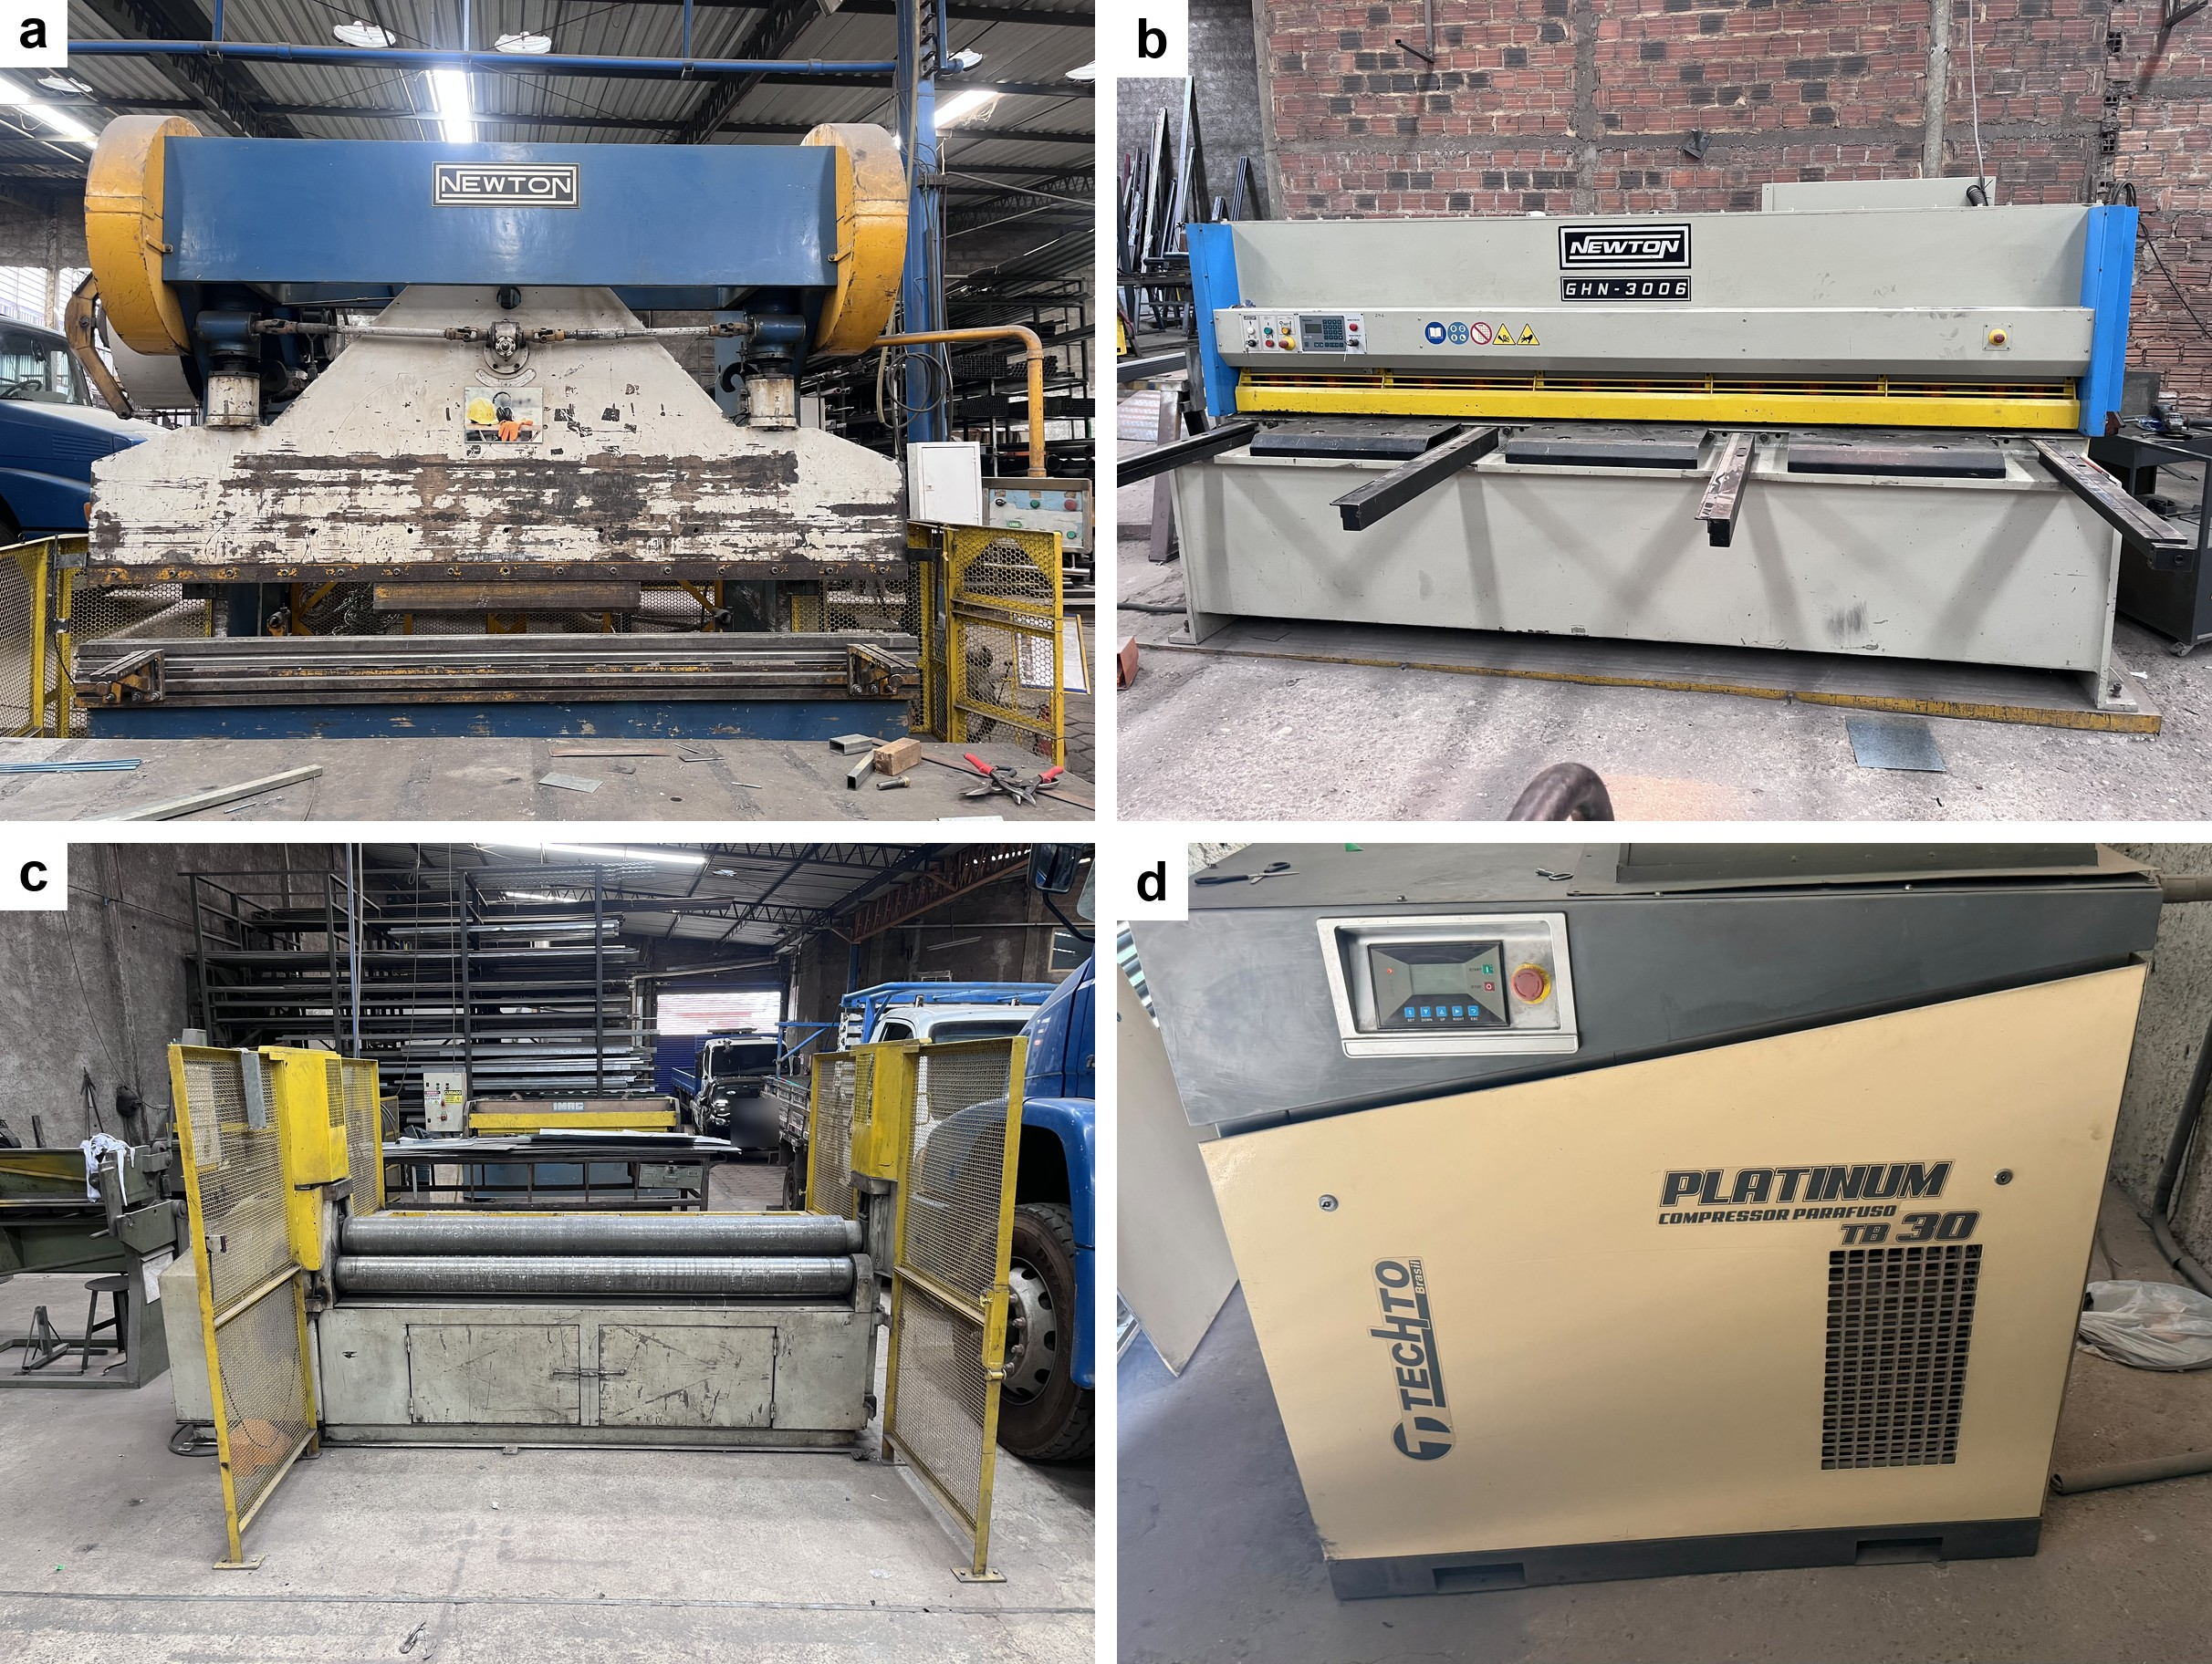
\includegraphics[width=\textwidth]{campo/fig19_maquinas.jpg}
\fonte{elaborado pelo próprio autor.}
\legenda{(a) dobradeira Newton PDM; (b) guilhotina hidráulica Newton GHN-3006; (c) calandra piramidal Vega CPVG2050X14; (d) compressor de parafuso Techto TB~30, fechado. Fotos de 2 de novembro de 2026. Em (c), a placa de um veículo e um logotipo, ao fundo, foram desfocados.}
\end{figure}

\begin{figure}[!htb]
\centering
\caption{Planta esquemática do galpão da coleta em campo}\label{fig:planta}
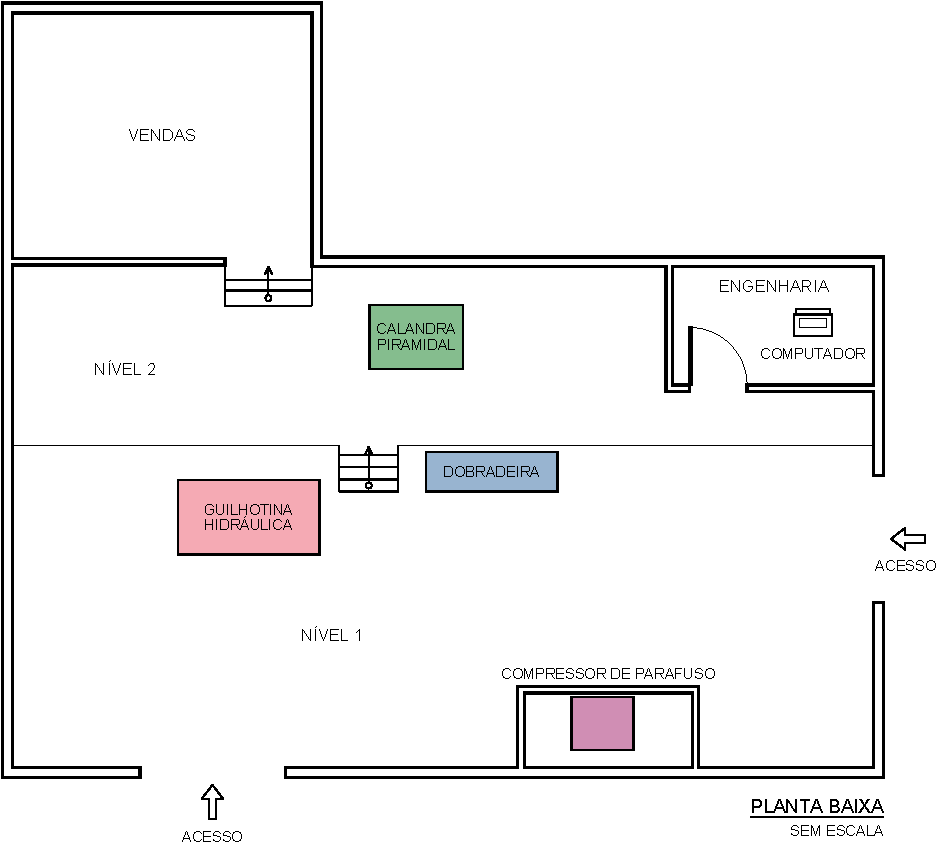
\includegraphics[width=\textwidth]{fig21_planta_local.pdf}
\fonte{elaborado pelo próprio autor.}
\legenda{planta sem escala, com as proporções de um esboço do autor. A linha fina entre os níveis 1 e 2 marca a mudança de nível do piso. Nas escadas, a linha começa num círculo e termina em seta no sentido da subida. As setas externas indicam as duas entradas do galpão. Cada máquina tem, em tom claro, a cor que a identifica nas Figuras~\ref{fig:ruido}, \ref{fig:espectros}, \ref{fig:injecao} e~\ref{fig:ap1}. O transmissor e o \textit{gateway} foram levados de uma máquina a outra e não têm posição fixa na planta.}
\end{figure}

A coleta teve duas rodadas. A primeira foi das \campoInicioDobradeiraUm\ às \campoFimCompressorUm, com um ciclo a cada \campoCicloUm~s, e a segunda, das \campoInicioCalandraDois\ às \campoFimGuilhotinaDois, com um ciclo a cada \campoCicloDois~s, depois de uma tentativa na dobradeira durante os reinícios do transmissor, das \reiniciosInicio\ às \reiniciosFim. Em cada ciclo, o transmissor enviou uma telemetria e uma janela de sinal bruto de \SI{0,512}{\second}, de modo que as janelas cobrem de \campoCoberturaUm~\% a \campoCoberturaDois~\% do tempo de cada ensaio. A calandra e a guilhotina foram medidas nas duas rodadas, com \campoIntervaloCalandra\ e \campoIntervaloGuilhotina\ entre os inícios dos dois ensaios de cada uma. Na segunda rodada, a dobradeira não teve sinal bruto, porque o transmissor, alimentado desde a manhã por uma bateria que não tinha sido carregada antes da coleta, reiniciou a cada ciclo por queda de tensão. Nos ensaios seguintes, ele foi alimentado por um carregador portátil. A temperatura do sensor, informada na telemetria, teve mediana de \campoTempRodadaUmMin~\si{\celsius} a \campoTempRodadaUmMax~\si{\celsius} nos ensaios da primeira rodada e de \campoTempRodadaDoisMin~\si{\celsius} a \campoTempRodadaDoisMax~\si{\celsius} nos da segunda, já com o carregador.

Os trechos analisados excluem a partida dos motores e o tempo em que a gravação continuou depois do fim da operação (Tabela~\ref{tab:ensaios}). Eles foram delimitados em 2 de novembro, nas análises exploratórias (seção~\ref{sec:preliminares}), e o registro das hipóteses já trazia o número de janelas de cada ensaio.

\begin{table}[!htb]
\centering\small
\caption{Ensaios da coleta em campo de 2 de novembro de 2026}\label{tab:ensaios}
\begin{tabular}{@{}>{\raggedright\arraybackslash}p{38mm}>{\raggedright\arraybackslash}p{46mm}c>{\raggedright\arraybackslash}p{27mm}r@{}}
\toprule
Máquina & Motor & Rodada & Trecho analisado & Janelas \\
\midrule
Dobradeira & placa ilegível & 1 & \campoInicioDobradeiraUm\ a \campoFimDobradeiraUm & \campoJanelasDobradeiraUm \\
Guilhotina hidráulica & \SI{9,2}{\kilo\watt} (\num{12,5}~cv), \SI{1760}{r/min} & 1 & \campoInicioGuilhotinaUm\ a \campoFimGuilhotinaUm & \campoJanelasGuilhotinaUm \\
 & & 2 & \campoInicioGuilhotinaDois\ a \campoFimGuilhotinaDois & \campoJanelasGuilhotinaDois \\
Calandra piramidal & \SI{2,2}{\kilo\watt} (\num{3}~cv), \SI{1715}{r/min} & 1 & \campoInicioCalandraUm\ a \campoFimCalandraUm & \campoJanelasCalandraUm \\
 & & 2 & \campoInicioCalandraDois\ a \campoFimCalandraDois & \campoJanelasCalandraDois \\
Compressor de parafuso & \SI{22}{\kilo\watt} & 1 & \campoInicioCompressorUm\ a \campoFimCompressorUm & \campoJanelasCompressorUm \\
Motor desligado & & 1 & \campoInicioMotorParado\ a \campoFimMotorParado & \campoJanelasMotorParado \\
\midrule
Total & & & & \campoJanelas \\
\bottomrule
\end{tabular}
\fonte{elaborada pelo próprio autor.}
\nota{horários locais (UTC$-$3) de 2 de novembro de 2026. Os dois motores com placa legível são de \SI{60}{\hertz}. Na calandra e no compressor, a potência é a do anúncio do fabricante para o mesmo modelo de máquina.}
\end{table}

Em todas as máquinas, o transmissor foi colado à carcaça do motor com fita dupla face 3M VHB de \SI{1}{\milli\meter} de espessura, trocada a cada ensaio (Figura~\ref{fig:montagem}). Entre a carcaça do motor e o sensor, a vibração passa pela fita dupla face, pelo invólucro do transmissor, pelas espumas entre o invólucro e o bloco eletrônico e pelas fitas que envolvem o bloco (seção~\ref{sec:sistema}). Na dobradeira, ele ficou deitado em cima da carcaça, com o eixo X do sensor na direção do eixo do motor. Na guilhotina, na calandra e no compressor, ficou na lateral da carcaça, com o eixo Y na direção do eixo do motor. A orientação dos outros dois eixos não foi padronizada, e na guilhotina o sensor ficou invertido de uma rodada para a outra. O operador levou o transmissor e o \textit{gateway} de uma máquina a outra, e o computador ficou parado na sala de engenharia (Figura~\ref{fig:planta}), ligado à rede Wi-Fi do local. A distância entre o transmissor e o \textit{gateway} não foi medida.

\begin{figure}[!htb]
\centering
\caption{Posição do transmissor e do \textit{gateway} na coleta em campo}\label{fig:montagem}
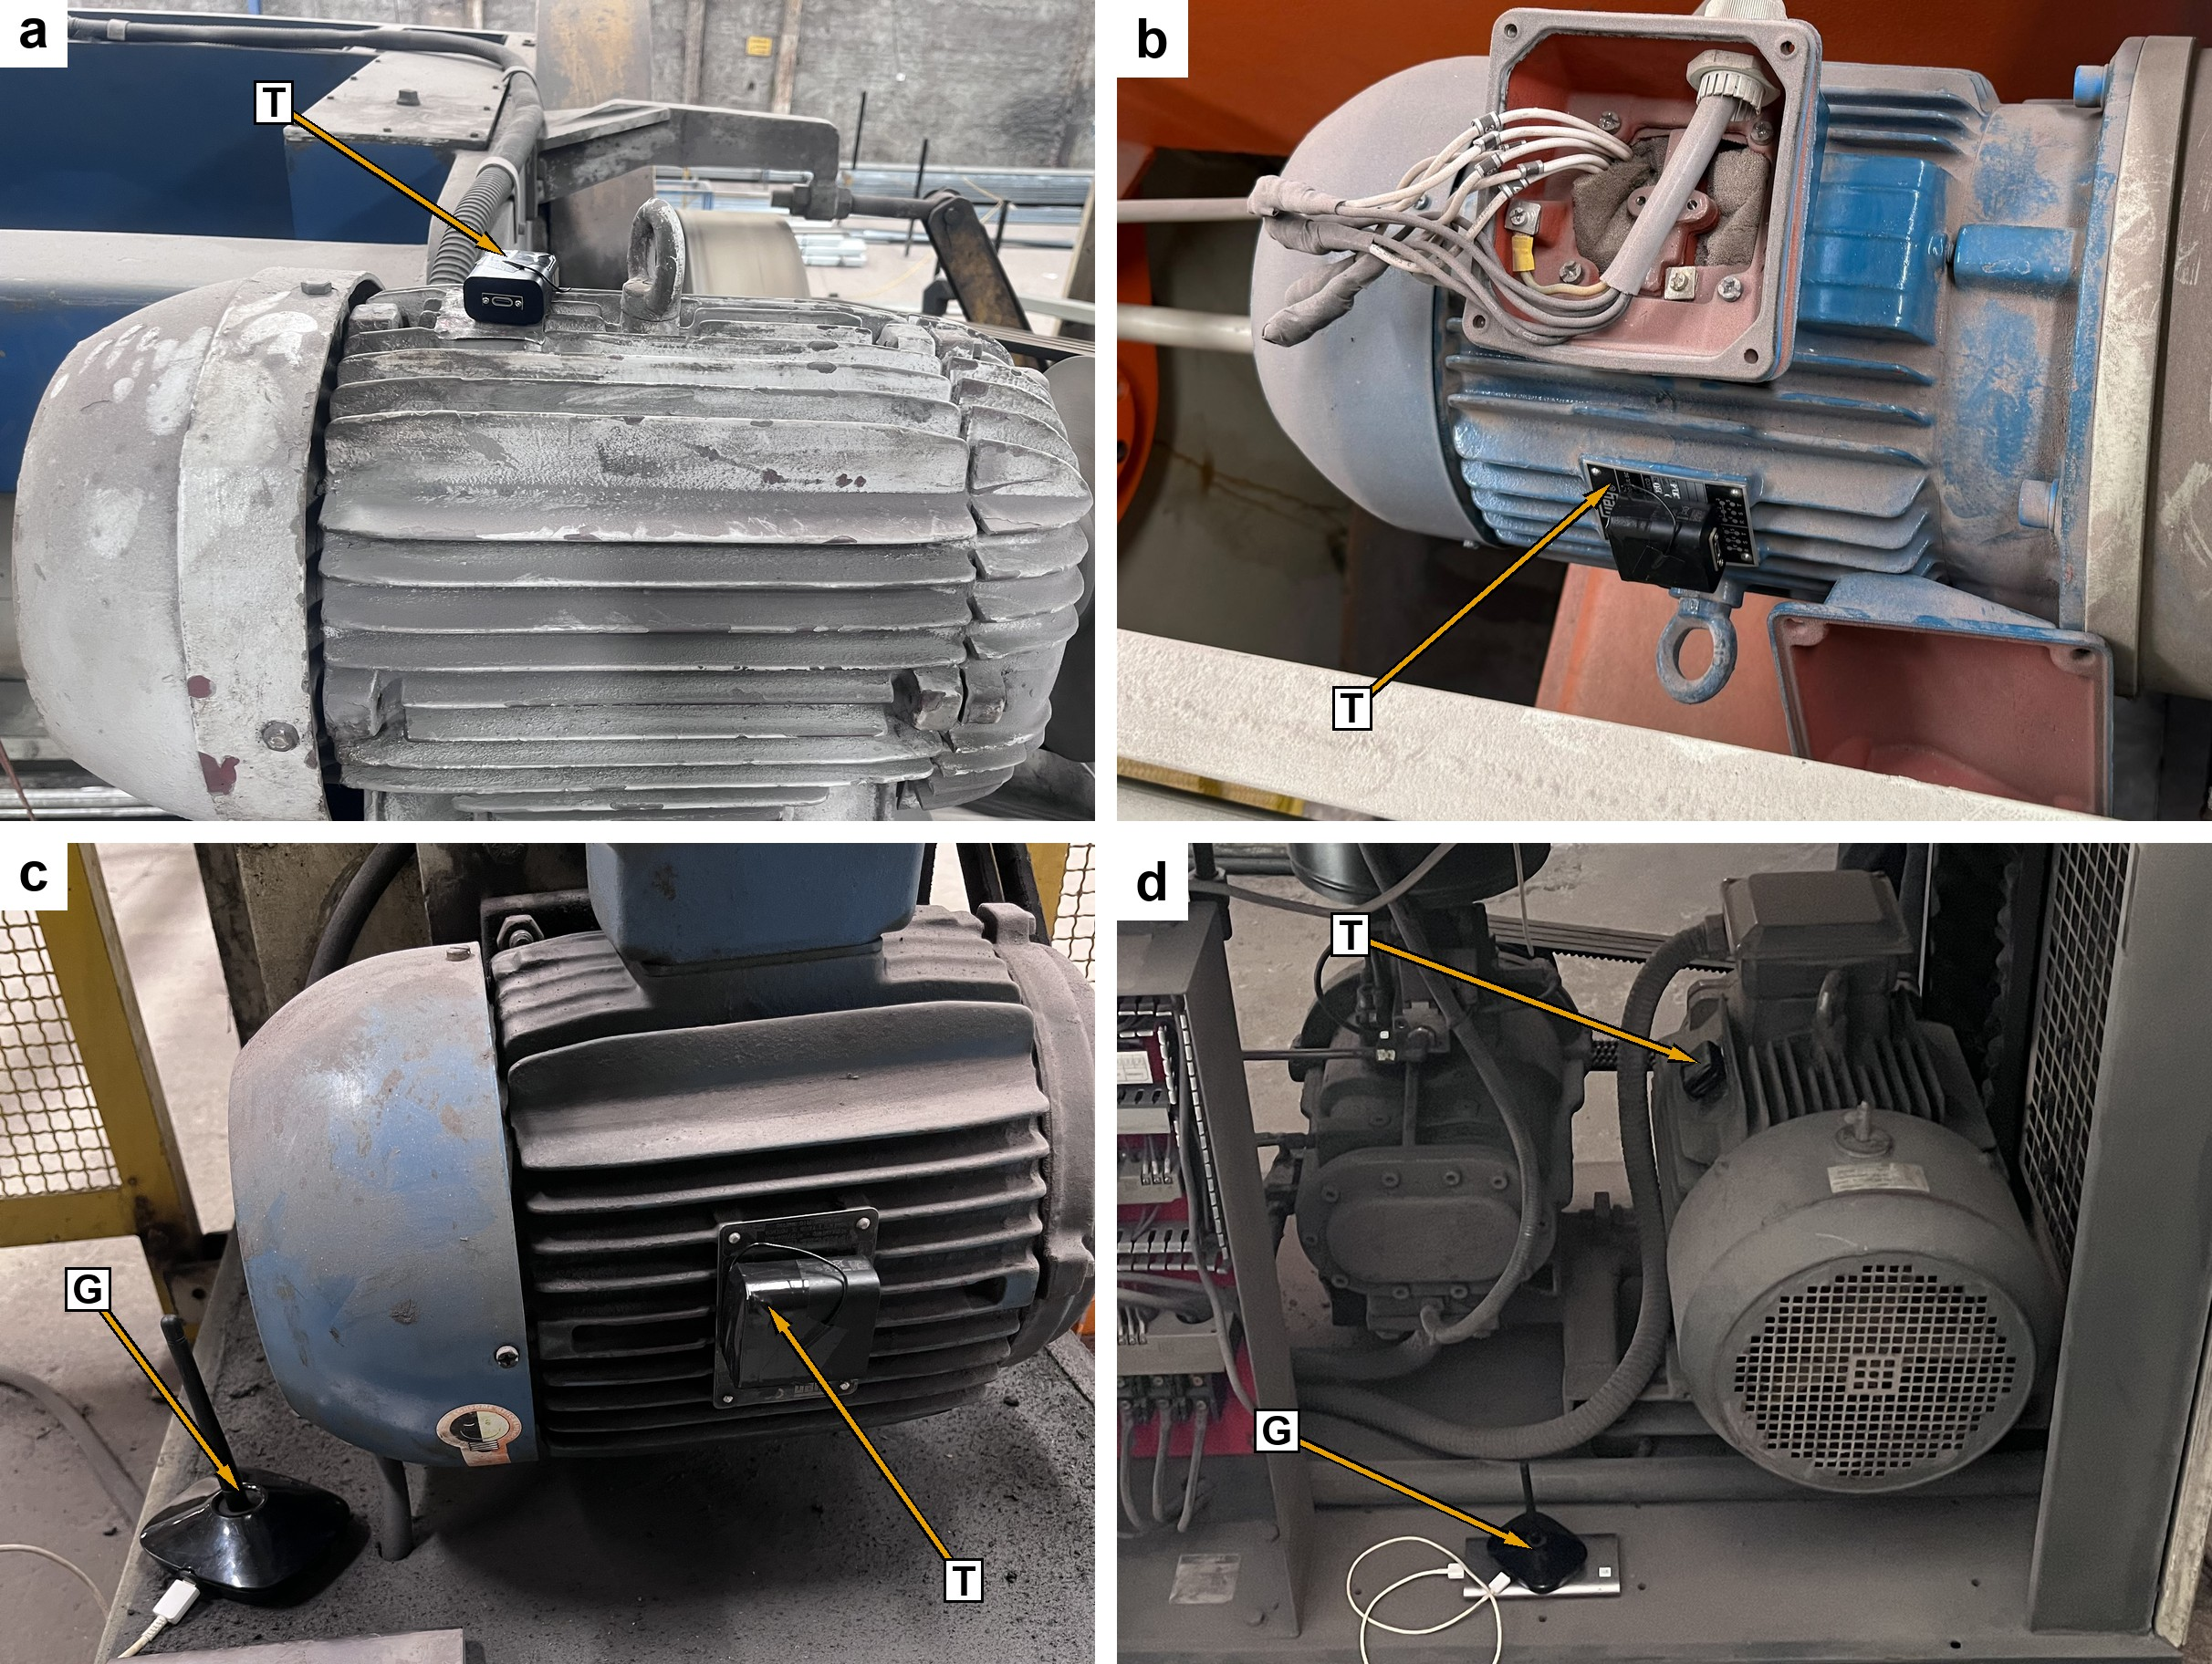
\includegraphics[width=\textwidth]{campo/fig16_montagem_campo.jpg}
\fonte{elaborado pelo próprio autor.}
\legenda{(a) dobradeira, às 12h45; (b) guilhotina, em horário não registrado; (c) calandra, às 13h17; (d) compressor, às 13h32. T indica o transmissor, e G, o \textit{gateway} na posição do momento da foto, apoiado sobre o carregador portátil que o alimentava.}
\end{figure}

Entre as duas rodadas, durante o almoço, o transmissor ficou ligado sobre uma mesa. Nesse período, a gravidade medida ficou constante, com o eixo Z na vertical, e o giroscópio não indicou movimento acima do próprio ruído. Por isso, as janelas adquiridas das \campoRepousoInicio\ às \campoRepousoFim\ foram usadas para estimar o ruído do sensor em repouso.

\section{Sistema de aquisição}\label{sec:sistema}

A coleta usou o sistema descrito na seção~\ref{cap:sistema}, com um transmissor e um \textit{gateway}. O transmissor usa um microcontrolador ESP32-C3, ligado a um módulo MPU-6050, com acelerômetro e giroscópio, por I2C e a um rádio Ra-02 (circuito SX1278) por SPI. O Ra-02 opera de \SIrange{410}{525}{\mega\hertz} \cite{aithinker2017ra02}. O \textit{gateway} usa um ESP32-S3 com o mesmo rádio, e a API e o banco de dados rodaram num computador levado ao local, na mesma rede Wi-Fi do \textit{gateway}.

O transmissor e o \textit{gateway} foram montados em invólucros reaproveitados (Figura~\ref{fig:dispositivos}). No transmissor, a placa ESP32-C3 Super Mini, o rádio, o módulo MPU-6050 e um módulo de carga de bateria TP4056 estão empilhados em um bloco, com as partes sensíveis protegidas por fita isolante líquida e fita de poliimida (Kapton). O invólucro é a carcaça vazia de um carregador, e dentro dele ficam o bloco, espumas entre o bloco e o invólucro e uma bateria de polímero de lítio de \SI{3,7}{\volt} e \SI{700}{\milli\ampere\hour}. A antena do rádio do transmissor é o fio que acompanha o módulo, no comprimento original. O invólucro do \textit{gateway} é a base de um sensor Kinect da primeira versão. Dentro dela ficam a placa de desenvolvimento do ESP32-S3, com o módulo coberto por fita de poliimida, e o rádio, em uma placa adaptadora, com os fios entre as duas placas agrupados por espaguete termorretrátil. Os dois rádios operam em \SI{433}{\mega\hertz}, e o do \textit{gateway} usou uma antena do tipo bastão feita para \SI{2,4}{\giga\hertz} e \SI{5}{\giga\hertz}, ligada ao módulo por um cabo com conector IPEX.

\begin{figure}[!htb]
\centering
\caption{Transmissor e \textit{gateway} usados na coleta em campo}\label{fig:dispositivos}
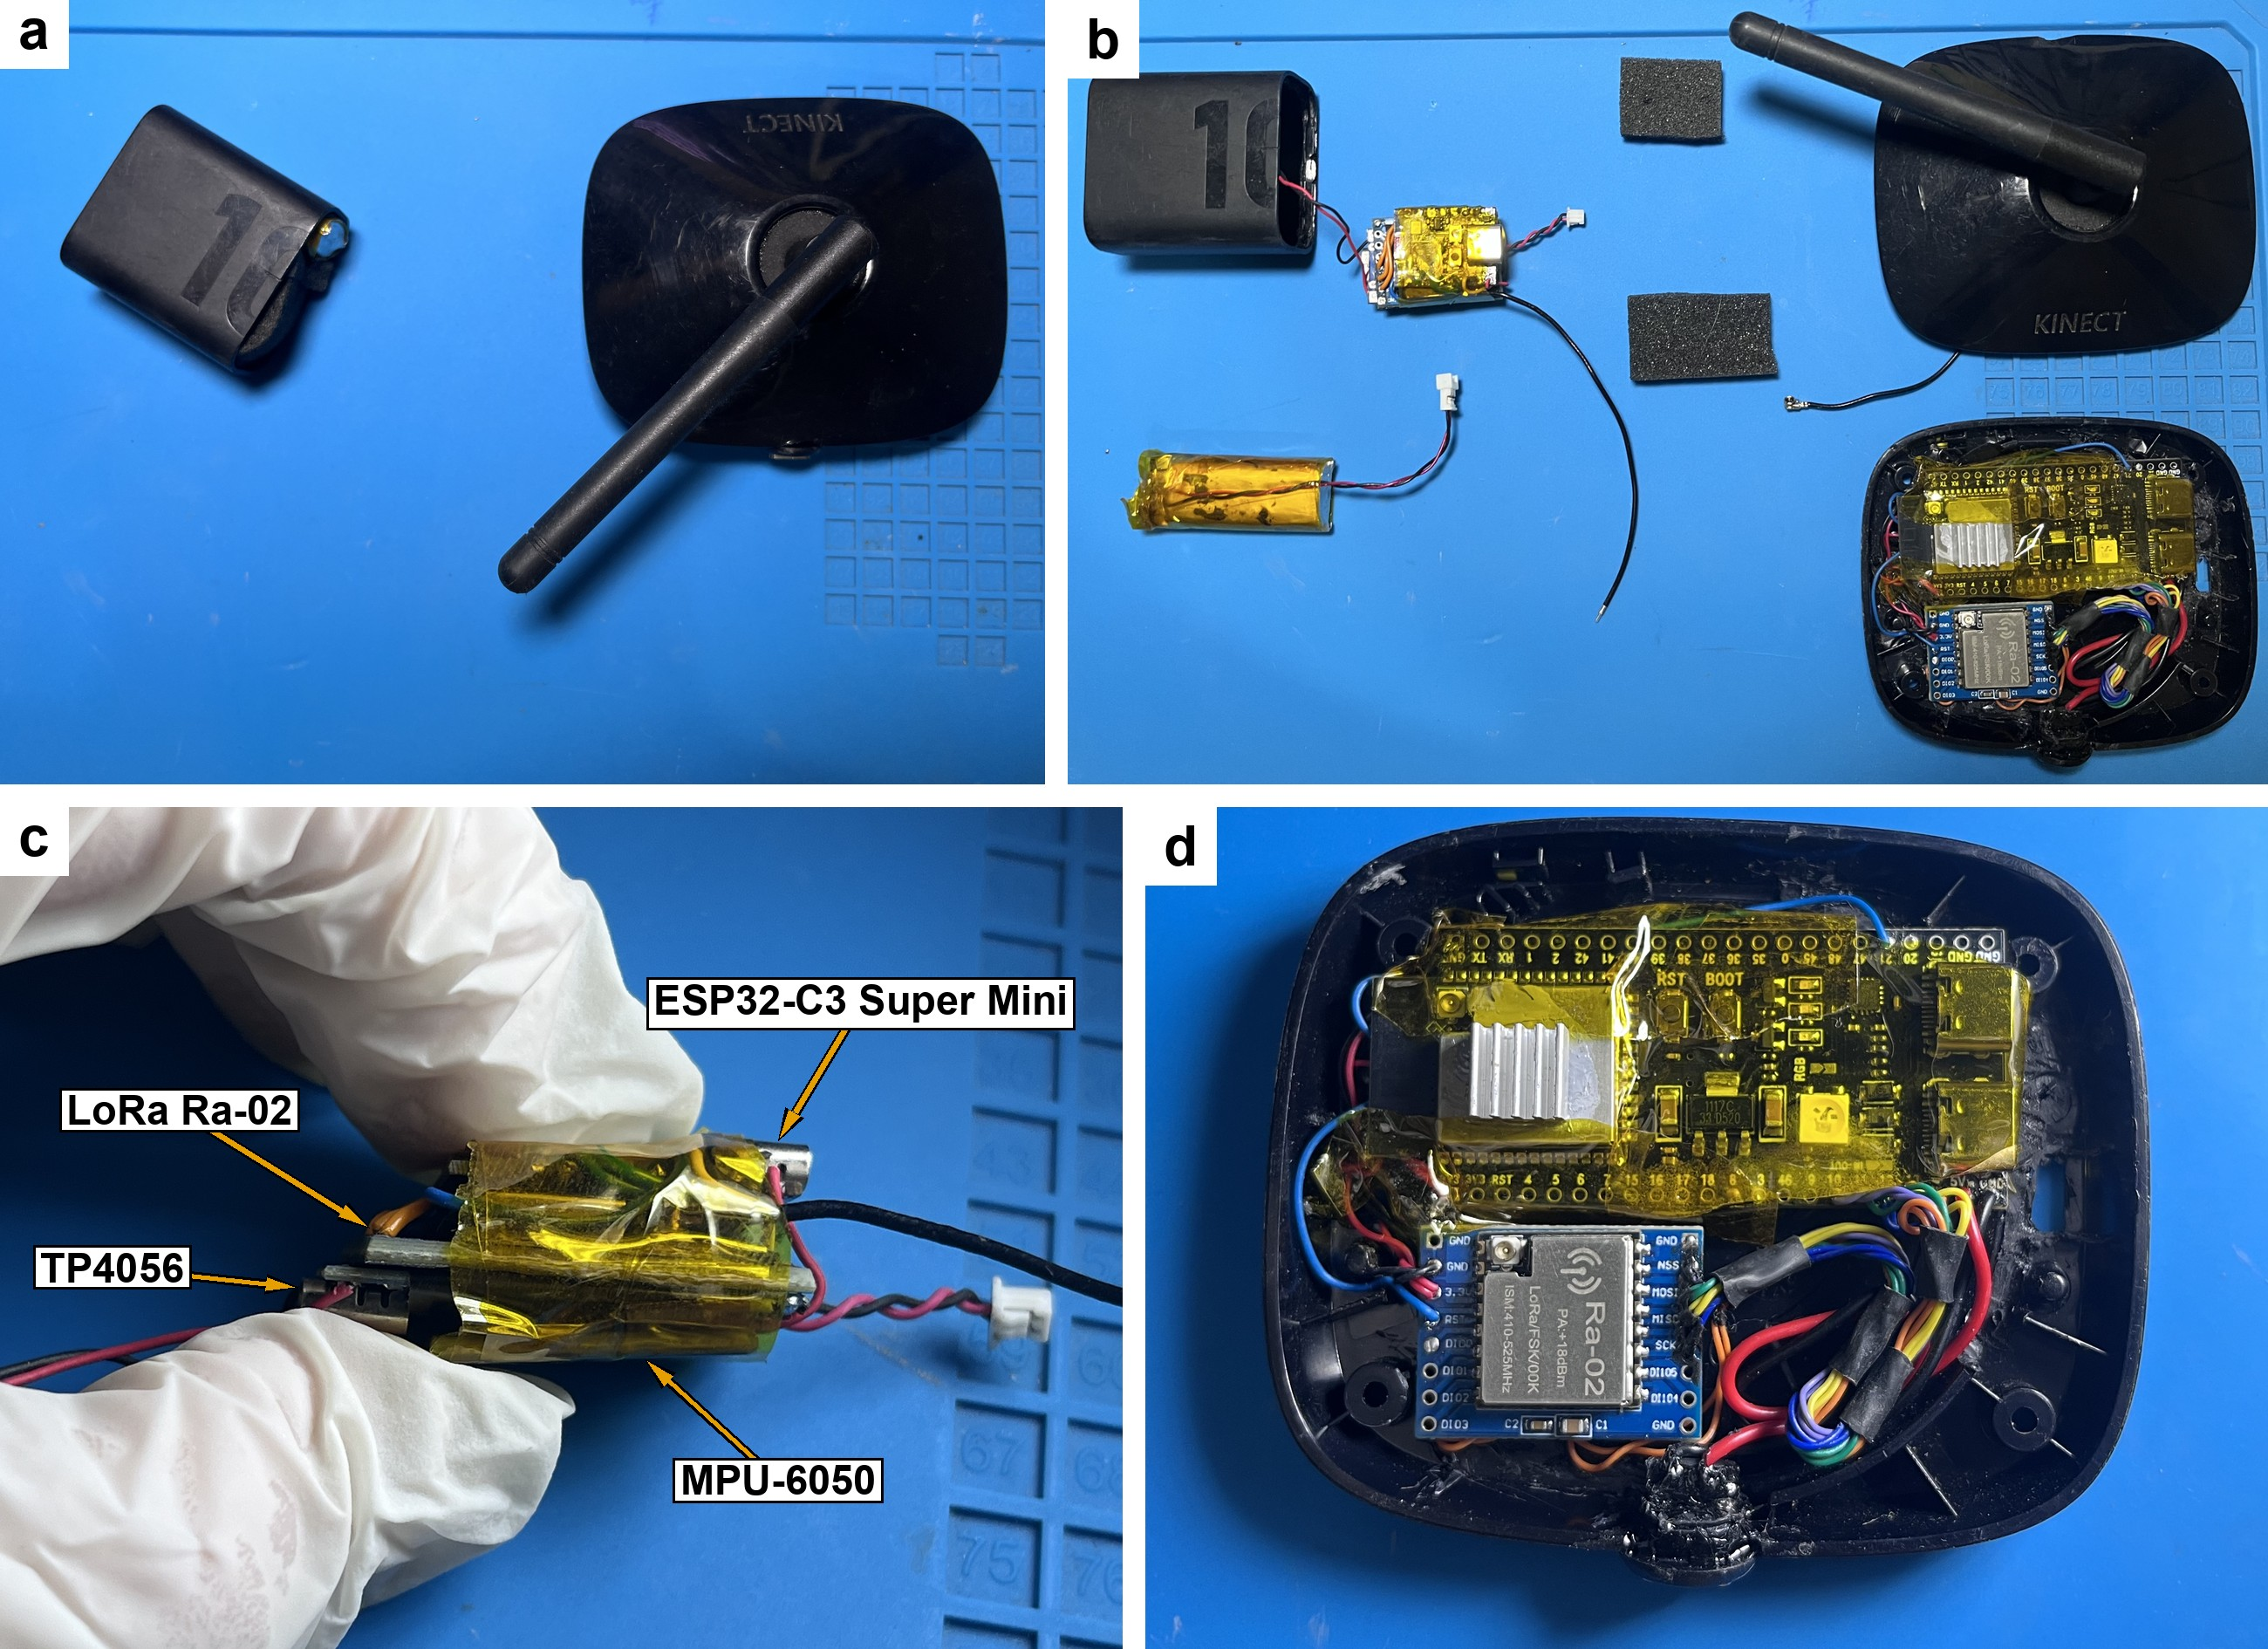
\includegraphics[width=\textwidth]{campo/fig20_dispositivos.jpg}
\fonte{elaborado pelo próprio autor.}
\legenda{(a) transmissor, à esquerda, e \textit{gateway}, à direita, fechados; (b) peças do transmissor, à esquerda e ao centro (invólucro, bloco eletrônico, bateria e espumas), e do \textit{gateway}, à direita (base e interior); (c) bloco eletrônico do transmissor, com os componentes indicados; (d) interior do \textit{gateway}, com a placa do ESP32-S3 coberta por fita de poliimida e o rádio na placa adaptadora. Fotos de 7 de novembro de 2026, cinco dias depois da coleta.}
\end{figure}

Os componentes eletrônicos dos dois dispositivos foram comprados no AliExpress. O preço pago não foi registrado, e a Tabela~\ref{tab:custo} dá o custo de uma compra nova, pela mediana dos preços anunciados para uma unidade em 9 de novembro de 2026, com os impostos. O pedido completo, de R\$~\num{140,83}, equivale a US\$~\num{25,60} pela taxa de câmbio de venda de 6 de novembro de 2026, de R\$~\num{5,5013} \cite{bcb2026ptax}. Desde 12 de maio de 2026, a compra de até US\$~\num{50} numa empresa certificada no Programa Remessa Conforme, como o AliExpress, tem imposto de importação zero \cite{receita2026manual}. Resta o ICMS, cuja carga nas remessas para o Piauí é de \SI{20}{\percent} \cite{piaui2025decreto}. Como o imposto é calculado por dentro, sobre o valor da compra somado ao próprio imposto, ele acrescenta \SI{25}{\percent} ao preço. A placa adaptadora do rádio do \textit{gateway} só é vendida em conjunto com o Ra-02, e o conjunto entrou na tabela no lugar do módulo avulso. Com o imposto, o transmissor custou R\$~\num{78,11} e o \textit{gateway}, R\$~\num{97,93}, sem a bateria, cujo preço não foi conferido.

\begin{table}[!htb]
\centering\small
\caption{Custo dos componentes do transmissor e do \textit{gateway} em 9 de novembro de 2026}\label{tab:custo}
\begin{tabular}{@{}llrrr@{}}
\toprule
Componente & Dispositivo & Anúncios & Preço (R\$) & Com ICMS (R\$) \\
\midrule
ESP32-C3 Super Mini & transmissor & \num{21} & \num{17,89} & \num{22,36} \\
Ra-02 (SX1278, \SI{433}{\mega\hertz}) & transmissor & \num{35} & \num{23,99} & \num{29,99} \\
Módulo MPU-6050 (GY-521) & transmissor & \num{39} & \num{13,69} & \num{17,11} \\
Módulo de carga TP4056 & transmissor & \num{13} & \num{6,92} & \num{8,65} \\
Bateria LiPo de \SI{3,7}{\volt} e \SI{700}{\milli\ampere\hour} & transmissor & 0 & \multicolumn{2}{c}{não cotada} \\
\addlinespace
\textit{Subtotal do transmissor} & & & \num{62,49} & \num{78,11} \\
\midrule
ESP32-S3 N16R8 (DevKitC-1) & \textit{gateway} & \num{19} & \num{31,29} & \num{39,11} \\
Ra-02 com placa adaptadora (conjunto) & \textit{gateway} & 1 & \num{27,99} & \num{34,99} \\
Antena de \num{2,4} e \SI{5}{\giga\hertz} com cabo IPEX & \textit{gateway} & \num{3} & \num{19,06} & \num{23,83} \\
\addlinespace
\textit{Subtotal do gateway} & & & \num{78,34} & \num{97,93} \\
\midrule
Total & & & \num{140,83} & \num{176,04} \\
\bottomrule
\end{tabular}
\fonte{elaborada pelo próprio autor, com preços do AliExpress e alíquotas de \citeonline{receita2026manual} e \citeonline{piaui2025decreto}.}
\nota{preço: mediana dos anúncios de uma unidade, de vendedores com envio do exterior, sem as ofertas de primeira compra; a coluna Anúncios dá quantos entraram na mediana. O frete foi considerado zero, porque a maioria dos anúncios o oferecia grátis. O conjunto do Ra-02 com placa adaptadora tem um só anúncio, de R\$~\num{27,99} na página do produto, com preço cheio de R\$~\num{56,00}. A consulta coincidiu com a campanha promocional de 11 de novembro. Com ICMS: carga de \SI{20}{\percent} calculada por dentro, igual a \SI{25}{\percent} do preço, e imposto de importação zero. Ficaram fora os invólucros reaproveitados, as fitas, as espumas e o computador da API.}
\end{table}

O sensor do módulo respondeu ao registrador de identificação (\texttt{WHO\_AM\_I}) com o valor \texttt{0x74}, diferente do \texttt{0x68} indicado no mapa de registradores do MPU-6050 \cite{invensense2012rm}, e a marcação do chip não foi conferida. O \textit{firmware} aceita os dois valores e, com \texttt{0x74}, usa o perfil MPU6515, em que o sensor foi configurado com faixa de $\pm\SI{4}{g}$ no acelerômetro, $\pm\SI{250}{\degree\per\second}$ no giroscópio e filtro passa-baixas digital interno de \SI{184}{\hertz} \cite{invensense2012rm}. A banda de \SI{184}{\hertz} é a nominal do mapa de registradores, e a resposta em frequência do sensor deste módulo não foi medida. O sensor amostra os seis canais a \SI{1}{\kilo\hertz} e guarda as amostras na FIFO, que o \textit{firmware} esvazia em lotes; assim, o espaçamento entre amostras é dado pelo relógio do sensor (seção~\ref{sec:sis-transmissor}). Cada janela tem \num{512} amostras por canal. O \textit{firmware} estima a taxa de amostragem de cada janela e, quando o desvio em relação a \SI{1}{\kilo\hertz} passa de \SI{2}{\percent}, marca a telemetria com código de diagnóstico e envia a janela com a taxa estimada.

Na coleta, o transmissor enviou em cada ciclo a telemetria e a janela de sinal bruto, no perfil padrão da rajada, com fator de espalhamento 7 e banda de \SI{250}{\kilo\hertz} (seção~\ref{sec:sis-protocolo}). A potência de transmissão foi de \campoPotenciaTx~dBm, abaixo do máximo do módulo em \SI{433}{\mega\hertz}, de \SI{18 \pm 1}{dBm} \cite{aithinker2017ra02}, e foi ajustada pelo rádio, como as demais mudanças de configuração (seção~\ref{sec:sis-configuracao}).

\section{Conjuntos de dados exportados}\label{sec:dados}

Os dados foram exportados do banco da API em modo somente leitura, e o resumo SHA-256 de cada janela foi conferido na exportação. O conjunto principal tem as \campoJanelas\ janelas e as \campoLeituras\ telemetrias dos trechos da Tabela~\ref{tab:ensaios}. Dois conjuntos complementares descrevem a medição em repouso e o enlace de rádio. O primeiro tem as \campoJanelasRepouso\ janelas com o transmissor sobre a mesa, e o segundo, \campoRajadas\ rajadas do histórico de eventos do \textit{gateway}, das \campoRajadasInicio\ às \campoRajadasFim, com o número de fragmentos recebidos e a duração de cada uma. Esse histórico guarda só os eventos mais recentes, e as rajadas anteriores às \campoRajadasInicio, inclusive as da dobradeira e da primeira rodada da guilhotina, não estão nele. O resumo SHA-256 do conjunto principal foi gravado no registro das hipóteses antes do cálculo (seção~\ref{sec:hipoteses}) e conferido no início de cada análise.

\section{Descritores}\label{sec:descritores}

As amostras do acelerômetro foram convertidas para $g$ pela faixa configurada, e a média de cada eixo foi removida em cada janela. A velocidade foi obtida por integração no domínio da frequência \cite{brandt2014}, sem janela de ponderação, com cada coeficiente $A_k$ da transformada discreta de Fourier da aceleração, na frequência $f_k$, dividido por $\mathrm{j}2\pi f_k$ e com os coeficientes fora da faixa de \SIrange{10}{184}{\hertz} anulados. O limite superior é o do filtro do sensor. A velocidade eficaz nessa faixa não é a de banda larga da norma, que vai até \SI{1000}{\hertz}, e não serve para classificar as máquinas nas zonas de severidade.

A rotação $f_r$ de cada janela foi estimada pelo maior pico do espectro da aceleração somado nos três eixos, com janela de Hann e preenchimento com zeros até \num{16} vezes o tamanho da janela, na faixa de $\pm\SI{2,5}{\hertz}$ em torno de um valor de busca fixado para cada máquina. Os valores de busca vieram das análises exploratórias (seção~\ref{sec:preliminares}): \campoBuscaDobradeiraUm~Hz na dobradeira e na calandra, \campoBuscaGuilhotinaUm~Hz na guilhotina e \campoBuscaCompressorUm~Hz no compressor. Nas três primeiras, a faixa de busca contém as rotações nominais das placas da guilhotina e da calandra. O compressor não tem dados de placa, e o valor de busca supõe que o pico perto de \SI{60}{\hertz} seja a rotação de um motor de dois polos. Com janelas de \SI{0,512}{\second}, a resolução do espectro é de \SI{1,95}{\hertz}, e o preenchimento com zeros não separa essa linha da frequência da rede elétrica, de \SI{60}{\hertz}.

Como a orientação do sensor mudou entre ensaios, os seis descritores de cada janela não dependem do sentido nem da ordem dos eixos:
\begin{itemize}
  \item $d_1$: velocidade eficaz de \SIrange{10}{184}{\hertz}, a maior entre os três eixos, em \si{\milli\meter\per\second};
  \item $d_2$: valor eficaz total da aceleração, raiz da soma dos quadrados dos três eixos, em $g$;
  \item $d_3$: maior curtose em excesso entre os três eixos;
  \item $d_4$: maior fator de crista entre os três eixos;
  \item $d_5$: amplitude eficaz da componente na rotação (ordem 1x) em velocidade, raiz da soma dos quadrados dos três eixos, em \si{\milli\meter\per\second};
  \item $d_6$: o mesmo para o dobro da rotação (ordem 2x).
\end{itemize}
As amplitudes $d_5$ e $d_6$ foram lidas no espectro com janela de Hann, corrigido para a perda de amplitude da janela. Nos detectores, $d_1$, $d_2$, $d_5$ e $d_6$ entram em logaritmo decimal.

\section{Detectores e limiar}\label{sec:detectores}

A linha de base de cada máquina é o conjunto de janelas de treino da operação normal, e um detector compara cada janela nova com ela. O detector principal é o Isolation Forest \cite{liu2008}, na implementação do scikit-learn \cite{scikitlearn2026}, com \num{100} árvores, subamostras do tamanho do treino até o máximo de \num{256} janelas e a semente do gerador de números aleatórios fixada em 0. O escore de cada janela é o oposto do valor devolvido por \texttt{score\_samples}, de modo que um escore maior indica janela mais afastada da linha de base. O detector secundário, usado só como descrição, é a regra por mediana e desvio absoluto mediano (MAD) \cite{leys2013}: o escore de uma janela é o maior valor, entre os seis descritores, de $|x - \tilde{x}|/(1{,}4826\,\mathrm{MAD})$, com a mediana $\tilde{x}$ e o MAD calculados no treino.

O limiar foi fixado para uma taxa de falso alarme de \SI{5}{\percent} na própria linha de base. As janelas de treino foram divididas em cinco blocos de janelas consecutivas, e cada bloco recebeu o escore de um modelo ajustado nos outros quatro. O limiar é o quantil de \SI{95}{\percent} desses escores, e o modelo usado na avaliação foi ajustado em todo o treino. Uma janela é marcada quando o escore passa do limiar.

\section{Assinaturas de desbalanceamento injetadas}\label{sec:injecao}

Como nenhuma máquina tinha falha conhecida, a fração de falhas detectadas não pode ser medida nesses dados. Para estimá-la em função da severidade, uma assinatura de desbalanceamento foi somada a janelas reais de operação normal que não participaram do treino. O desbalanceamento produz uma força que gira com o eixo, na frequência de rotação \cite{randall2011livro}, e por isso a assinatura foi somada aos dois eixos radiais do sensor, em quadratura:
\begin{equation}
a_{r1}(t) \leftarrow a_{r1}(t) + A_a \sin(2\pi f_r t + \varphi), \qquad a_{r2}(t) \leftarrow a_{r2}(t) + A_a \cos(2\pi f_r t + \varphi),
\label{eq:injecao}
\end{equation}
em que $f_r$ é a rotação medida na própria janela, $\varphi$ é uma fase sorteada por janela e $A_a = \sqrt{2}\,A_v\,2\pi f_r$ é a amplitude de aceleração que corresponde à velocidade eficaz $A_v$ acrescentada em cada eixo. $A_v$ variou de 0 a \SI{2,8}{\milli\meter\per\second}, em passos de \SI{0,05}{\milli\meter\per\second}. Na calandra e na guilhotina, o treino foi a primeira rodada, e o teste, a segunda. Na dobradeira e no compressor, que têm uma rodada, o treino foi a primeira metade das janelas, em ordem de tempo, e o teste, a segunda.

Para cada amplitude, a fração marcada é a fração das janelas de teste com escore do detector principal acima do limiar do treino. A amplitude com \SI{50}{\percent} das janelas marcadas, $A_{50}$, foi obtida por interpolação linear entre os pontos da grade. Uma assinatura do dobro da rotação, somada ao eixo axial, foi calculada apenas como descrição. A assinatura somada não reproduz a modulação, a variação de fase ao longo do tempo nem o caminho de transmissão de uma falha real, e uma falha real pode ser mais fácil ou mais difícil de detectar que a assinatura.

\section{Desbalanceamento real em base pública}\label{sec:base-publica}

Como a coleta não teve máquina com falha, o detector também foi avaliado numa base pública com desbalanceamento real, medida numa bancada de laboratório da Fraunhofer-Gesellschaft (\citeauthoronline{mey2020}, \citeyear{mey2020}, \citeyear{mey2022dados}). A base, na versão 151.3, tem licença Creative Commons Atribuição 4.0, que exige a citação dos autores, do título e do identificador digital de objeto (DOI) e a indicação das modificações. Neste trabalho, as modificações são o uso exclusivo das medições 0D e 0E a 4E, o recorte por tensão constante e por rotação, a divisão em janelas e o corte em \SI{184}{\hertz}, descritos a seguir. Os dados modificados não foram redistribuídos. Como o repositório original estava fora do ar, as medições foram obtidas da cópia do Internet Archive de 14 de dezembro de 2022.

Na bancada, um motor de corrente contínua com comutação eletrônica (WEG~UE~511~T) gira um eixo de \SI{12}{\milli\meter}, apoiado num mancal de rolamento em bloco de aço galvanizado. O desbalanceamento é uma massa presa a um suporte de náilon impresso em 3D, montado logo atrás do bloco do mancal, em cinco níveis: 0, com o suporte sem massa, e 1 a 4, com \SIlist{45,9;60,7;75,5;152,1}{\milli\meter\gram}. Três acelerômetros uniaxiais PCB M607A11, no bloco do mancal e na fixação do motor, foram amostrados a \SI{4096}{\hertz}, e a base não informa a posição de cada canal nem a unidade da vibração. A rotação muda em degraus de tensão de \SI{20}{\second}, percorridos duas vezes. Nos arquivos de desenvolvimento, 0D a 4D, a tensão vai de \SIrange{2,0}{10,05}{\volt} em passos de \SI{0,05}{\volt}, e nos de avaliação, 0E a 4E, de \SIrange{4,0}{8,1}{\volt} em passos de \SI{0,1}{\volt}. Entre as medições D e E, o suporte do desbalanceamento foi desmontado e remontado.

Os primeiros \num{50000} valores de cada arquivo foram descartados, como no artigo da base \cite{mey2020}. Depois do descarte, o número de amostras de 0E e de 4E coincidiu com o informado nos cadernos dos autores da base, conferência prevista no registro de H4 (Apêndice~\ref{ap:registro}). O sinal foi dividido em janelas consecutivas, sem sobreposição, de \num{2048} amostras, que duram \SI{0,5}{\second} e têm resolução de \SI{2,0}{\hertz}, perto das janelas do transmissor, de \SI{0,512}{\second} e \SI{1,95}{\hertz}. Entraram as janelas com tensão constante e rotação média de \SIrange{1750}{1850}{r/min}, faixa que contém a rotação estimada na dobradeira, na guilhotina e na calandra, de \rotacaoRpmMin\ a \rotacaoRpmMax~r/min. As duas primeiras janelas de cada degrau, em que a rotação ainda muda, foram descartadas. Os três canais de vibração fazem o papel dos três eixos do sensor, com a média removida em cada janela. Para reproduzir a banda do transmissor, os coeficientes acima de \SI{184}{\hertz} foram anulados antes do cálculo de $d_2$, $d_3$ e $d_4$, e a velocidade de $d_1$ vai de \SIrange{10}{184}{\hertz}, como na seção~\ref{sec:descritores}. A rotação $f_r$ de cada janela é o pico do espectro da mesma seção, com valor de busca igual à média da rotação medida pela bancada na janela. Como a unidade da vibração não é informada, $d_1$, $d_2$, $d_5$ e $d_6$ ficam na unidade dos canais. O detector usa esses descritores em logaritmo, e um fator de escala comum ao treino e ao teste não muda o resultado.

O detector principal e o limiar são os da seção~\ref{sec:detectores}, com treino em todas as janelas do arquivo 0D que passaram pelo pré-processamento. O falso alarme é a fração das janelas de 0E marcadas, e a fração marcada em cada nível de desbalanceamento é a das janelas de 1E a 4E, com intervalos de confiança como na seção~\ref{sec:analise}. No download, o tamanho e o CRC-32 de cada arquivo foram conferidos com o índice do arquivo compactado, e o SHA-256 de cada um foi gravado antes do cálculo de qualquer descritor.

A bancada tem motor pequeno, eixo de \SI{12}{\milli\meter} e nenhuma carga, e os três sensores são uniaxiais e ficam em dois pontos, enquanto o transmissor usa um sensor triaxial num ponto. Nenhum ruído foi acrescentado ao sinal da base, e o sensor do transmissor não foi modelado. Por isso, H4 avalia o método de detecção diante de uma falha real, e o desempenho do dispositivo em campo continua avaliado só por H1 a H3.

\section{Hipóteses e critérios}\label{sec:hipoteses}

A hipótese central é que, com uma linha de base construída só com operação normal, a cadeia de aquisição de baixo custo da seção~\ref{sec:sistema}, do sensor à API, detecta mudanças de vibração do tamanho que a norma considera significativas, com falso alarme limitado entre rodadas da mesma máquina. Ela se desdobra em três hipóteses derivadas, H1 a H3 (Quadro~\ref{tab:hipoteses}). Uma quarta hipótese, H4, avalia o detector diante do desbalanceamento real da base pública (seção~\ref{sec:base-publica}). H1 a H3 e os critérios de decisão foram registrados em 6 de novembro de 2026, antes de qualquer cálculo que as avaliasse, e não mudaram depois dos resultados. Em 7 de novembro, uma emenda acrescentou H4 e duas análises posteriores aos resultados de H2 e H3, AP1 e AP2 (seção~\ref{sec:res-posteriores}), antes do cálculo delas. Outra emenda, também anterior ao cálculo de H4, trocou a versão da base pública, porque a versão 151.2 ficou indisponível. Em 8 de novembro, depois de todos esses resultados, uma terceira emenda acrescentou quatro análises posteriores, AP3 a AP6, sem hipótese nova e sem mudança de critério (seção~\ref{sec:res-posteriores}). O Apêndice~\ref{ap:registro} descreve cada registro e o que já se conhecia antes dele.

\begin{quadro}[!htb]
\centering\small
\caption{Hipóteses e critérios de corroboração e de refutação}\label{tab:hipoteses}
\begin{tabular}{@{}>{\raggedright\arraybackslash}p{36mm}>{\raggedright\arraybackslash}p{62mm}>{\raggedright\arraybackslash}p{46mm}@{}}
\toprule
Hipótese & Critério de corroboração & Critério de refutação \\
\midrule
H1. Falso alarme entre rodadas & Na calandra e na guilhotina, com treino na primeira rodada, o detector principal marca até \SI{10}{\percent} das janelas da segunda rodada, com limite superior do intervalo de até \SI{20}{\percent} & Fração marcada acima de \SI{20}{\percent} em ao menos uma das máquinas \\
\addlinespace
H2. Menor mudança detectável & Em todos os ensaios com ao menos \num{25} janelas, a menor mudança detectável em $d_1$ fica abaixo de \SI{0,7}{\milli\meter\per\second} & Menor mudança detectável de \SI{0,7}{\milli\meter\per\second} ou mais em ao menos um desses ensaios \\
\addlinespace
H3. Detecção da assinatura injetada & Nas quatro máquinas, $A_{50}$ fica abaixo de \SI{0,7}{\milli\meter\per\second}, e a correlação de Spearman entre a amplitude e a fração marcada é de \num{0,9} ou mais & $A_{50}$ de \SI{0,7}{\milli\meter\per\second} ou mais, ou não atingido até \SI{2,8}{\milli\meter\per\second}, ou correlação abaixo de \num{0,9}, em ao menos uma máquina \\
\addlinespace
H4. Desbalanceamento real em base pública & Com treino em 0D, o detector principal marca até \SI{10}{\percent} das janelas de 0E, com limite superior do intervalo de até \SI{20}{\percent}, e \SI{50}{\percent} ou mais das janelas em cada nível, de 1E a 4E & Fração marcada acima de \SI{20}{\percent} em 0E, ou abaixo de \SI{50}{\percent} em ao menos um nível \\
\bottomrule
\end{tabular}
\fonte{elaborado pelo próprio autor.}
\nota{em H1 e em H4, os resultados entre os dois critérios deixam a hipótese indeterminada. Em H2, a regra de alarme é $d_1$ acima do quantil de \SI{95}{\percent} de $d_1$ no próprio ensaio, e a menor mudança detectável é a diferença entre esse quantil e a mediana: o aumento da mediana que leva metade das janelas acima do limiar, com a dispersão mantida.}
\end{quadro}

A ISO 20816-3 avalia a vibração pelo valor da vibração de banda larga e pela mudança desse valor \cite{iso208163_2022}. Na série ISO 10816, que a ISO 20816-3 substituiu, uma variação de \SI{25}{\percent} do limite superior da zona B, para mais ou para menos, é considerada significativa e pede investigação da causa \cite{schwirzer2002}. Neste trabalho, o tamanho de referência é \SI{0,7}{\milli\meter\per\second}, \SI{25}{\percent} do limite B/C de \SI{2,8}{\milli\meter\per\second} do grupo 2 em fundação rígida, o menor limite B/C da norma. Pela edição de 2022 da norma, a guilhotina e a calandra, com \SI{9,2}{\kilo\watt} e \SI{2,2}{\kilo\watt}, ficam abaixo da potência mínima, de \SI{15}{\kilo\watt}, e nelas o valor serve só de referência de tamanho. A edição de 2026 não fixa potência mínima no escopo, e os limites de zona dessa edição não foram consultados (seção~\ref{sec:fund-norma}). O compressor, com \SI{22}{\kilo\watt}, está no grupo 2, de \SIrange{15}{300}{\kilo\watt}.

A hipótese central é corroborada quando H1, H2 e H3 o são. H4, avaliada na base pública, não entra nessa decisão.

\subsection{Análises exploratórias anteriores ao registro}\label{sec:preliminares}

Os mesmos dados foram examinados em 2 e 5 de novembro, antes do registro. Nessas análises exploratórias, com outro conjunto de descritores, o Isolation Forest e a regra por mediana e MAD foram treinados em uma rodada e aplicados à outra e marcaram, respectivamente, de \registroExplIfMin~\% a \registroExplIfMax~\% e de \registroExplMadMin~\% a \registroExplMadMax~\% das janelas. A velocidade eficaz da calandra e da guilhotina também foi comparada entre as rodadas, e a rotação e as ordens de cada máquina foram estimadas. Os limites de \SI{10}{\percent} e de \SI{20}{\percent} de H1 foram fixados depois dessas frações, e por isso a avaliação de H1 não é independente das análises exploratórias. Essas análises originaram as hipóteses e não as corroboram. A avaliação de H1 a H3 usou somente os dados de 2 de novembro, e não houve nova coleta.

\subsection{Procedimentos de validade}\label{sec:validade-proc}

O delineamento adotou procedimentos para cada um dos quatro aspectos de validade descritos por \citeonline[p.~153--154]{runeson2009}, e as ameaças que permaneceram são avaliadas na seção~\ref{sec:limitacoes}. Para a validade de construto, os descritores, os detectores e os critérios foram definidos antes do cálculo, a velocidade foi comparada com o critério da norma com a diferença de banda declarada, e a injeção da assinatura foi conferida numa janela sintética de fase conhecida (seção~\ref{sec:res-ap1}). Para a validade interna, os critérios foram registrados antes do cálculo, e a avaliação incluiu controles descritivos: o sentido inverso de H1, a regra por mediana e MAD, o motor desligado e o sensor em repouso. Para a validade externa, o detector foi aplicado também a uma base pública de laboratório com desbalanceamento real (seção~\ref{sec:base-publica}). Para a confiabilidade, os dados foram conferidos pelo resumo SHA-256 (seção~\ref{sec:dados}), as sementes do gerador de números aleatórios e as versões das bibliotecas foram fixadas, e os números do texto foram gravados pelas próprias análises.

\section{Análise estatística}\label{sec:analise}

As frações de janelas marcadas têm intervalo de confiança de \SI{95}{\percent} por reamostragem em blocos de cinco janelas consecutivas, com \num{2000} réplicas e percentis, porque janelas próximas no tempo não são independentes. Não houve correção de multiplicidade. A integridade dos dados foi descrita pelas lacunas na sequência das telemetrias, pela taxa de amostragem estimada pelo transmissor e pela conferência do SHA-256. Os cálculos foram feitos em Python \ambPython, com NumPy \ambNumpy, SciPy \ambScipy\ e scikit-learn \ambSklearn, e a avaliação de H4, também com pandas \ambPandas. A documentação do Isolation Forest citada neste trabalho \cite{scikitlearn2026} é a da versão 1.9.1, consultada em 29 de outubro de 2026. Os dados da coleta e o código do sistema e das análises estão nos repositórios do projeto.\plano{Endereço público e licença dos repositórios e dos dados: a definir pelo autor.}

\chapter{Resultados}\label{cap:resultados}

As \campoJanelas\ janelas dos trechos analisados chegaram completas, e o valor eficaz total da aceleração nas máquinas em operação ficou de \sinalRazaoMin\ a \sinalRazaoMax\ vezes o do sensor em repouso. Nenhuma das quatro hipóteses foi corroborada. H1 ficou \hUmVeredito, com \hUmFracaoCalandra~\% das janelas da segunda rodada da calandra marcadas pelo detector treinado na primeira, e H2, H3 e H4 foram refutadas. A menor mudança detectável na velocidade eficaz passou de \SI{0,7}{\milli\meter\per\second} em três dos cinco ensaios avaliados. Com a assinatura de desbalanceamento, a fração marcada não chegou a \SI{50}{\percent} até \SI{2,8}{\milli\meter\per\second} em nenhuma das quatro máquinas. Na base pública, o detector marcou de \hQuatroFracaoTres~\% a \hQuatroFracaoQuatro~\% das janelas com desbalanceamento real e também \hQuatroFracaoZero~\% das janelas sem desbalanceamento medidas depois da remontagem do suporte. Nas análises posteriores, com as sementes de 0 a \num{99} do detector, H1 seria corroborada com \apTresVereditoUmCorroborada\ delas e indeterminada ou refutada com as demais, e H4 seria refutada com \apTresVereditoQuatroRefutada. Em três das quatro máquinas, o escore do detector ficou abaixo do limiar mesmo com os três descritores alterados pela assinatura fora da faixa do treino.

\section{Aquisição e integridade dos dados}\label{sec:res-aquisicao}

Nos trechos analisados, a sequência das \campoLeituras\ telemetrias \campoLacunasTexto, e o resumo SHA-256 de todas as janelas conferiu na exportação. A taxa de amostragem estimada pelo transmissor ficou entre \campoTaxaMin~Hz e \campoTaxaMax~Hz, com desvio máximo de \campoDesvioTaxaMax~\% em relação a \SI{1}{\kilo\hertz}, abaixo do limite de \SI{2}{\percent} do \textit{firmware}. A intensidade do sinal recebido (RSSI) das telemetrias ficou entre \campoRssiMin~dBm e \campoRssiMax~dBm.

Em repouso sobre a mesa, a densidade de ruído do acelerômetro, média de \SIrange{20}{150}{\hertz}, foi de \ruidoDensidadeX~µg/$\sqrt{\text{Hz}}$ no eixo X, \ruidoDensidadeY~µg/$\sqrt{\text{Hz}}$ no Y e \ruidoDensidadeZ~µg/$\sqrt{\text{Hz}}$ no Z (Figura~\ref{fig:ruido}a). Os dois eixos horizontais ficaram abaixo dos \ruidoDatasheet~µg/$\sqrt{\text{Hz}}$ da folha de dados do MPU-6050 \cite{invensense2011ps}. O eixo Z, vertical sobre a mesa, tem linhas abaixo de \SI{200}{\hertz} ausentes em X e em Y, o que é compatível com vibração da mesa somada ao ruído do sensor. Acima de cerca de \SI{200}{\hertz}, a densidade diminui nos três eixos, o que é compatível com o filtro interno de banda nominal de \SI{184}{\hertz}. Em velocidade, o ruído em repouso corresponde a \ruidoVelocidade~mm/s no descritor $d_1$, mediana das janelas.

\begin{figure}[!htb]
\centering
\caption{Ruído do acelerômetro em repouso e valor eficaz em cada ensaio}\label{fig:ruido}
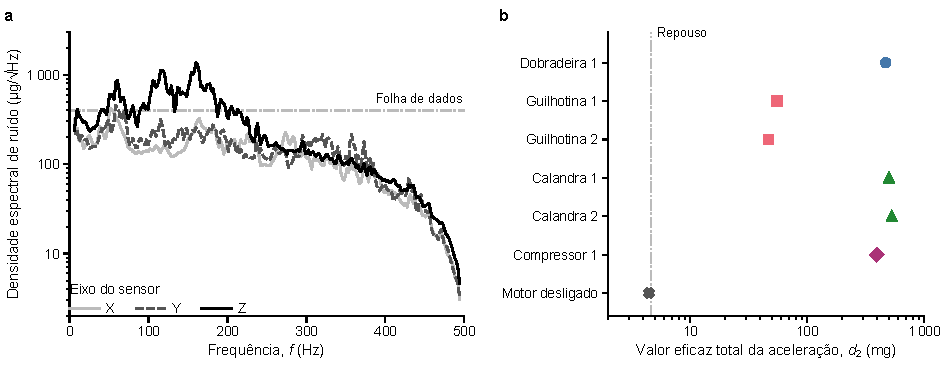
\includegraphics{fig_ruido.pdf}
\fonte{elaborado pelo próprio autor.}
\legenda{\textbf{a}, densidade espectral de ruído de cada eixo do sensor, pelo método de Welch com janela de Hann de \num{512} amostras, média das \campoJanelasRepouso\ janelas com o transmissor sobre a mesa; a linha horizontal marca os \ruidoDatasheet~µg/$\sqrt{\text{Hz}}$ da folha de dados do MPU-6050. \textbf{b}, mediana, entre as janelas de cada ensaio, do valor eficaz total da aceleração ($d_2$); o número depois do nome da máquina é a rodada, e a linha vertical marca o valor em repouso. Eixo vertical de \textbf{a} e eixo horizontal de \textbf{b} em escala logarítmica.}
\end{figure}

O valor eficaz total da aceleração, mediana das janelas de cada ensaio, foi de \sinalRmsGuilhotinaDois~mg a \sinalRmsCalandraDois~mg nas máquinas em operação, contra \ruidoRmsTotal~mg em repouso (Figura~\ref{fig:ruido}b). A guilhotina teve o menor valor, de \sinalRazaoGuilhotinaDois\ a \sinalRazaoGuilhotinaUm\ vezes o de repouso. No trecho com o motor desligado, o valor foi de \sinalRmsMotorParadoDecimal~mg, \sinalRazaoMotorParadoDecimal\ vez o de repouso.

Das \reiniciosInicio\ às \reiniciosFim, o transmissor reiniciou por queda de tensão da bateria, e esse intervalo é chamado aqui de período de reinícios. O período começa com as primeiras reinicializações e termina na hora da última das \rajadasSequenciaUmPeriodo\ rajadas enviadas no primeiro ciclo depois de uma inicialização. Fora dele, \rajadasForaCompletas\ das \rajadasFora\ rajadas do histórico de eventos do \textit{gateway} chegaram completas (\rajadasForaPct~\%), isto é, com os \num{26} fragmentos depois de no máximo três tentativas. A rajada completa durou \rajadasDuracaoMediana~s, mediana entre elas. A fração de rajadas completas variou com a RSSI da telemetria do mesmo ciclo (Figura~\ref{fig:enlace}). Com RSSI de \SI{-80}{dBm} ou mais, \rajadasAcimaOitentaPct~\% chegaram completas, de \SI{-110}{dBm} a \SI{-80}{dBm}, \rajadasCentoDezOitentaCompletas\ das \rajadasCentoDezOitenta, e abaixo de \SI{-110}{dBm}, \rajadasAbaixoCentoDezCompletas\ de \rajadasAbaixoCentoDez. Como a posição do transmissor e do \textit{gateway} em cada rajada não foi anotada, os dados não permitem atribuir à distância a variação da RSSI.

Das \rajadasFalhasTotal\ rajadas incompletas registradas no histórico de 2 de novembro, \rajadasFalhasReinicio\ ocorreram durante o período de reinícios. Das \rajadasForaIncompletas\ fora desse período, \rajadasForaSemFragmento\ não tiveram nenhum fragmento recebido. Nenhuma rajada incompleta ocorreu nos trechos analisados, e nenhuma janela desses trechos ficou com fragmento ausente.

\begin{figure}[!htb]
\centering
\caption{Rajadas completas em função da intensidade do sinal recebido}\label{fig:enlace}
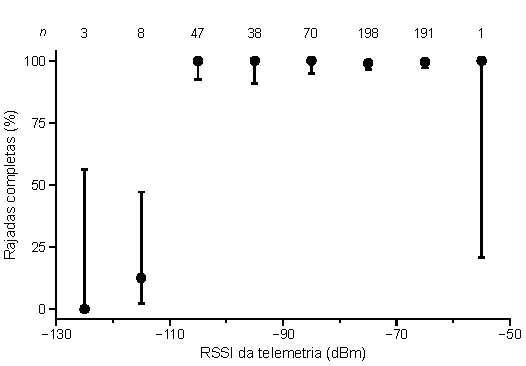
\includegraphics{fig_enlace.pdf}
\fonte{elaborado pelo próprio autor.}
\legenda{fração das rajadas do histórico de eventos do \textit{gateway} que chegaram com os \num{26} fragmentos, depois de no máximo três tentativas, em faixas de \SI{10}{dB} da RSSI da telemetria do mesmo ciclo, com o ponto no centro da faixa. As barras mostram o intervalo de confiança de \SI{95}{\percent} de \citeonline{wilson1927}, e $n$, acima do gráfico, é o número de rajadas da faixa. Exclui o período de reinícios por bateria, das \reiniciosInicio\ às \reiniciosFim.}
\end{figure}

\section{Linha de base das máquinas}\label{sec:res-base}

A rotação estimada na dobradeira, na guilhotina e na calandra ficou entre \rotacaoRpmMin\ e \rotacaoRpmMax~r/min, perto da velocidade síncrona de \SI{1800}{r/min} de um motor de quatro polos em \SI{60}{\hertz}, e a do compressor, em \rotacaoRpmCompressorUm~r/min, perto dos \SI{3600}{r/min} de um motor de dois polos. Só a guilhotina e a calandra têm placa legível, e o número de polos da dobradeira e do compressor é uma suposição (seção~\ref{sec:descritores}). Na guilhotina e na calandra, a rotação ficou acima da nominal de placa, de \SI{1760}{r/min} e \SI{1715}{r/min}, o que é compatível com a operação sem carga, em que o escorregamento é menor que o nominal \cite{chapman2012}. Entre as janelas de um mesmo ensaio, a rotação estimada teve desvio-padrão de \rotacaoDesvioMin~Hz a \rotacaoDesvioMax~Hz, ou de \rotacaoDesvioPctMin~\% a \rotacaoDesvioPctMax~\% da velocidade síncrona. Pela mediana das janelas, o escorregamento estimado foi de no máximo \escorregamentoCalandraDois~\%, na segunda rodada da calandra, e de \escorregamentoGuilhotinaDois~\% na segunda rodada da guilhotina, com a rotação acima da síncrona por menos que o desvio-padrão entre janelas de qualquer ensaio.

Nos espectros médios dos seis ensaios, \picosTotal\ linhas ficaram acima de dez vezes o nível mediano do espectro, \picosPrimeiraRodada\ delas nos ensaios da primeira rodada, mostrados na Figura~\ref{fig:espectros}. Uma linha foi associada a uma ordem da rotação quando ficou a até \picosTolerancia~Hz dela. Das \picosTotal\ linhas, \picosDiretos\ coincidem com ordens da rotação, \picosRebatidos\ coincidem com ordens acima de \SI{500}{\hertz} rebatidas pela amostragem a \SI{1}{\kilo\hertz} (equação do rebatimento, seção~\ref{sec:fund-aquisicao}) e \picosNaoIdentificados\ não foram associadas a uma ordem. As ordens rebatidas estão na guilhotina, \picosRebatidosGuilhotinaUm\ na primeira rodada (Figura~\ref{fig:espectros}b) e \picosRebatidosGuilhotinaDois\ na segunda, fora da figura. As linhas rebatidas são compatíveis com conteúdo acima de \SI{500}{\hertz} rebatido na amostragem, apesar do filtro interno de \SI{184}{\hertz}, que é digital \cite{invensense2012rm}.

\begin{figure}[!htb]
\centering
\caption{Espectro médio da aceleração na primeira rodada de cada máquina}\label{fig:espectros}
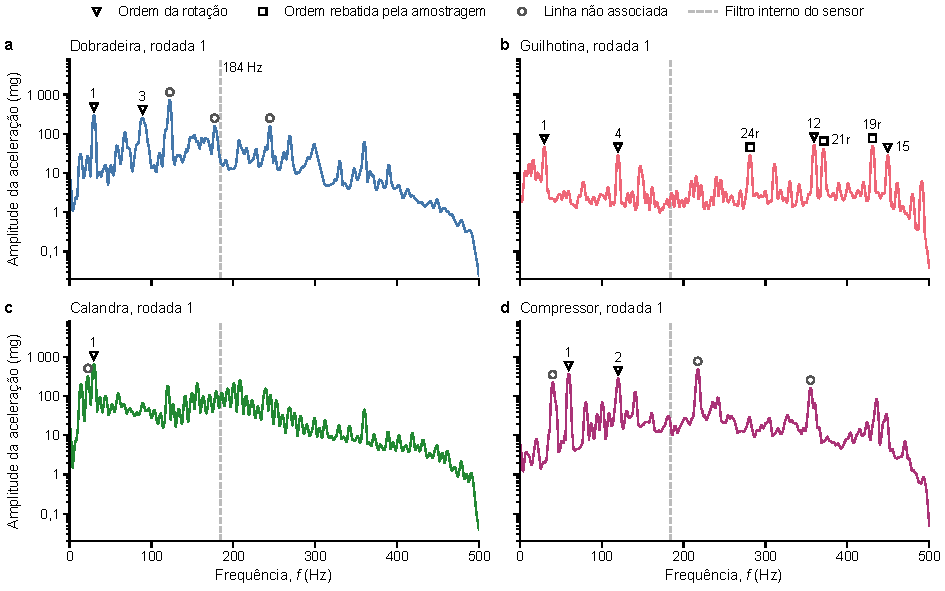
\includegraphics{fig_espectros.pdf}
\fonte{elaborado pelo próprio autor.}
\legenda{amplitude da aceleração com os três eixos somados, média das janelas do ensaio, com janela de Hann e preenchimento com zeros até quatro vezes o tamanho da janela; eixo vertical em escala logarítmica, comum aos quatro painéis. Os marcadores ficam sobre as linhas acima de dez vezes o nível mediano do espectro. Uma linha foi associada a uma ordem da rotação quando ficou a até \picosTolerancia~Hz dela, e o número junto ao marcador é a ordem, seguido de r quando a ordem passa de \SI{500}{\hertz} e aparece rebatida pela amostragem. A linha vertical marca a banda nominal de \SI{184}{\hertz} do filtro interno do sensor. \textbf{a}, dobradeira; \textbf{b}, guilhotina; \textbf{c}, calandra; \textbf{d}, compressor.}
\end{figure}

A velocidade eficaz de \SIrange{10}{184}{\hertz} foi maior na direção axial do que nas radiais na dobradeira, na calandra e no compressor, com medianas de \velAxialDobradeiraUm, \velAxialCalandraUm\ e \velAxialCompressorUm~mm/s (Figura~\ref{fig:eixos}). Na guilhotina, a direção axial teve o menor valor, e a maior velocidade, radial, teve mediana de \velMaxGuilhotinaUm~mm/s. As três medianas axiais passam do limite entre as zonas C e D do grupo 2 em fundação rígida, de \SI{4,5}{\milli\meter\per\second}, e as da dobradeira e da calandra passam também o de fundação flexível, de \SI{7,1}{\milli\meter\per\second} \cite{iso208163_2022}. Como a faixa de \SIrange{10}{184}{\hertz} está contida na de \SIrange{10}{1000}{\hertz} da norma, esses valores são limites inferiores da velocidade eficaz de banda larga no mesmo sinal. O sinal, porém, é o medido pelo transmissor depois da fita, do invólucro e das espumas, e a resposta dessa fixação não foi medida (seção~\ref{sec:ensaios}).

\begin{figure}[!htb]
\centering
\caption{Velocidade eficaz por direção em cada ensaio}\label{fig:eixos}
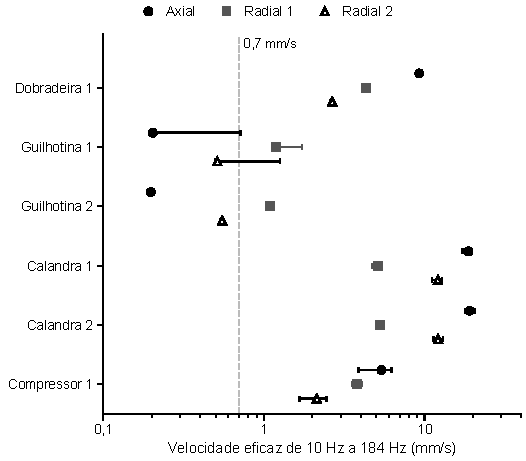
\includegraphics{fig_eixos.pdf}
\fonte{elaborado pelo próprio autor.}
\legenda{mediana (marcador) e intervalo interquartil (barra), entre as janelas de cada ensaio, da velocidade eficaz de \SIrange{10}{184}{\hertz} em cada eixo do sensor, identificado pela direção em relação ao eixo do motor; o número depois do nome da máquina é a rodada. A linha vertical marca o tamanho de referência de \SI{0,7}{\milli\meter\per\second} (seção~\ref{sec:hipoteses}). Eixo horizontal em escala logarítmica.}
\end{figure}

\section{Falso alarme entre rodadas}\label{sec:res-h1}

Treinado na primeira rodada, o detector principal marcou \hUmCalandraIFDireto~\% das janelas da segunda rodada da calandra, com intervalo de confiança de \SI{95}{\percent} de \hUmCalandraIFDiretoInf~\% a \hUmCalandraIFDiretoSup~\%, e \hUmGuilhotinaIFDireto~\% das janelas da segunda rodada da guilhotina. Na calandra, a fração ficou acima dos \SI{10}{\percent} do critério de corroboração e abaixo dos \SI{20}{\percent} do critério de refutação, e H1 ficou \hUmVeredito. O intervalo registrado reamostra só as janelas de teste. Com as sementes de 0 a \num{99} do detector, a fração marcada na calandra teve mediana de \apTresSementeCalandraMed~\%, abaixo dos \hUmFracaoCalandra~\% da semente 0, registrada, e H1 seria corroborada com \apTresVereditoUmCorroborada\ das \apTresSementes\ sementes (seção~\ref{sec:res-ap3}).

Entre as duas rodadas da calandra, várias condições da medição mudaram ao mesmo tempo. O transmissor foi colado de novo, com fita nova, a alimentação passou da bateria para o carregador portátil, e o intervalo entre ciclos passou de \campoCicloUm\ para \campoCicloDois~s. A temperatura do sensor, mediana da telemetria, passou de \campoTempCalandraUm\ para \campoTempCalandraDois~\si{\celsius}, e os inícios dos dois ensaios ficaram separados por \campoIntervaloCalandra. A mediana de $d_1$ variou \repetCalandraDif~\%, de \repetCalandraUm\ para \repetCalandraDois~mm/s. Na guilhotina, a fixação, a alimentação e o ciclo mudaram da mesma forma, a temperatura passou de \campoTempGuilhotinaUm\ para \campoTempGuilhotinaDois~\si{\celsius}, a mediana de $d_1$ variou \repetGuilhotinaDif~\%, de \repetGuilhotinaUm\ para \repetGuilhotinaDois~mm/s, e o sensor ficou invertido de uma rodada para a outra (seção~\ref{sec:ensaios}). Os dados não separam o efeito de cada uma dessas mudanças sobre a fração marcada.

No sentido inverso, com treino na segunda rodada, o detector principal marcou \hUmCalandraIFInverso~\% das janelas da primeira rodada da calandra e \hUmGuilhotinaIFInverso~\% das da guilhotina, que tem só \campoJanelasGuilhotinaUm\ janelas nessa rodada. A regra por mediana e MAD não marcou nenhuma janela no sentido direto e marcou \hUmCalandraMADInverso~\% e \hUmGuilhotinaMADInverso~\% no inverso. Os resultados do sentido inverso e da regra por MAD são descritivos e não entram no critério.

\section{Menor mudança detectável}\label{sec:res-h2}

A menor mudança detectável no descritor $d_1$ ficou abaixo de \SI{0,7}{\milli\meter\per\second} na dobradeira e na segunda rodada da guilhotina e acima desse valor no compressor e nas duas rodadas da calandra (Tabela~\ref{tab:h2}). Pelo critério registrado, H2 foi refutada. A menor mudança detectável não acompanhou o nível de $d_1$. A dobradeira, com mediana de \hDoisMedianaDobradeiraUm~mm/s, teve menor mudança detectável de \hDoisMmdDobradeiraUm~mm/s, e o compressor, com mediana de \hDoisMedianaCompressorUm~mm/s, de \hDoisMmdCompressorUm~mm/s.

\begin{table}[!htb]
\centering\small
\caption{Menor mudança detectável no descritor $d_1$ em cada ensaio da coleta de 2 de novembro de 2026}\label{tab:h2}
\begin{tabular}{@{}llrrrrr@{}}
\toprule
Máquina & Rodada & Janelas & Mediana & Quantil de \SI{95}{\percent} & \multicolumn{2}{c}{Menor mudança detectável} \\
\cmidrule(l){6-7}
 & & & (mm/s) & (mm/s) & (mm/s) & (\%) \\
\midrule
Dobradeira & 1 & \hDoisNDobradeiraUm & \hDoisMedianaDobradeiraUm & \hDoisQDobradeiraUm & \hDoisMmdDobradeiraUm & \hDoisRelDobradeiraUm \\
Guilhotina & 1 & \hDoisNGuilhotinaUm & \hDoisMedianaGuilhotinaUm & \hDoisQGuilhotinaUm & \hDoisMmdGuilhotinaUm & \hDoisRelGuilhotinaUm \\
Guilhotina & 2 & \hDoisNGuilhotinaDois & \hDoisMedianaGuilhotinaDois & \hDoisQGuilhotinaDois & \hDoisMmdGuilhotinaDois & \hDoisRelGuilhotinaDois \\
Calandra & 1 & \hDoisNCalandraUm & \hDoisMedianaCalandraUm & \hDoisQCalandraUm & \hDoisMmdCalandraUm & \hDoisRelCalandraUm \\
Calandra & 2 & \hDoisNCalandraDois & \hDoisMedianaCalandraDois & \hDoisQCalandraDois & \hDoisMmdCalandraDois & \hDoisRelCalandraDois \\
Compressor & 1 & \hDoisNCompressorUm & \hDoisMedianaCompressorUm & \hDoisQCompressorUm & \hDoisMmdCompressorUm & \hDoisRelCompressorUm \\
\bottomrule
\end{tabular}
\fonte{elaborada pelo próprio autor.}
\nota{a menor mudança detectável é a diferença entre o quantil de \SI{95}{\percent} e a mediana de $d_1$ no ensaio; em porcentagem, relativa à mediana. A primeira rodada da guilhotina, com menos de \num{25} janelas, não entra no critério de H2.}
\end{table}

A refutação de H2 não depende de poucas janelas. Na reamostragem por blocos da AP4, todas as réplicas das duas rodadas da calandra e do compressor ficaram acima de \SI{0,7}{\milli\meter\per\second}, e a menor mudança detectável da segunda rodada da guilhotina, abaixo desse valor na amostra, passou dele em \apQuatroAcimaGuilhotinaDois~\% das réplicas (seção~\ref{sec:res-ap4}). Pela mesma regra, a menor mudança detectável de $d_1$ com o sensor em repouso foi de \apCincoMmd~mm/s, e a dos cinco ensaios do critério ficou de \apCincoRazaoMin\ a \apCincoRazaoMax\ vezes esse valor (seção~\ref{sec:res-ap5}). A variação de $d_1$ entre janelas nas máquinas foi, portanto, maior que a do sensor parado. Ela reúne a vibração da máquina e a resposta da fixação do transmissor, e os dados não separam as duas.

A primeira rodada da guilhotina, que não entra no critério, teve a maior variação relativa, com quantil de \SI{95}{\percent} de \hDoisQGuilhotinaUm~mm/s para uma mediana de \hDoisMedianaGuilhotinaUm~mm/s. Os acionamentos da lâmina durante os ensaios não foram anotados, e os dados não permitem dizer se as janelas com $d_1$ mais alto coincidem com eles.

\section{Detecção das assinaturas injetadas}\label{sec:res-h3}

Com o detector principal, a fração marcada não chegou a \SI{50}{\percent} em nenhuma máquina até \SI{2,8}{\milli\meter\per\second} de assinatura em cada eixo radial (Figura~\ref{fig:injecao}). Entre todas as amplitudes da grade, a maior fração marcada foi de \hTresFracaoMaxCalandra~\% na calandra, \hTresFracaoMaxDobradeira~\% na dobradeira, \hTresFracaoMaxGuilhotina~\% na guilhotina e \hTresFracaoMaxCompressor~\% no compressor. Pelo critério registrado, H3 foi refutada.

A correlação de Spearman entre a amplitude e a fração marcada foi de \hTresRhoDobradeira\ na dobradeira, \hTresRhoGuilhotina\ na guilhotina, \hTresRhoCalandra\ na calandra e \hTresRhoCompressor\ no compressor. Na dobradeira e no compressor, as janelas marcadas foram de \hTresJanelasMinDobradeira\ a \hTresJanelasMaxDobradeira\ das \hTresTesteDobradeira\ janelas de teste e de \hTresJanelasMinCompressor\ a \hTresJanelasMaxCompressor\ das \hTresTesteCompressor\ em toda a grade de amplitudes, e as correlações negativas refletem a oscilação dessas poucas janelas.

Nenhuma das dez florestas de cada máquina, treinadas com as sementes de 0 a 9 do gerador de números aleatórios, chegou a \SI{50}{\percent} de janelas marcadas. A regra por mediana e MAD, que sem assinatura já marcava \hTresMadZeroDobradeira~\% das janelas de teste da dobradeira, chegou a \SI{50}{\percent} só nessa máquina, com \hTresMadDobradeira~mm/s. A assinatura do dobro da rotação no eixo axial, calculada como descrição, chegou a \SI{50}{\percent} só na guilhotina, com \hTresDoisXGuilhotina~mm/s.

\begin{figure}[!htb]
\centering
\caption{Fração de janelas marcadas em função da amplitude da assinatura de desbalanceamento}\label{fig:injecao}
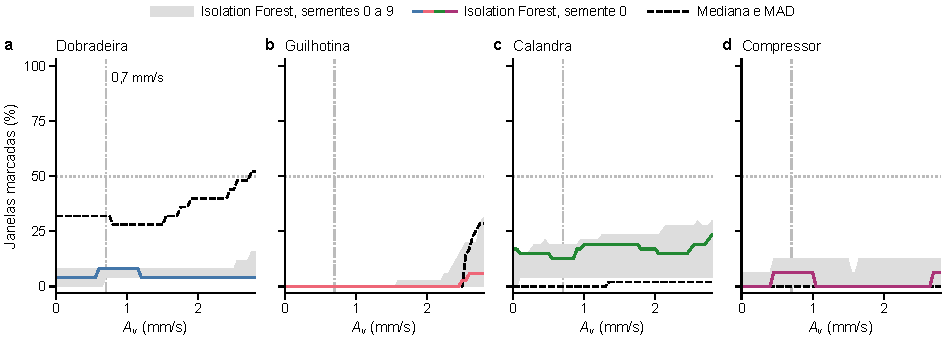
\includegraphics{fig_injecao.pdf}
\fonte{elaborado pelo próprio autor.}
\legenda{assinatura na rotação somada aos dois eixos radiais em quadratura, com velocidade eficaz $A_v$ em cada eixo, às janelas de teste da dobradeira (\textbf{a}, \hTresTesteDobradeira\ janelas), da guilhotina (\textbf{b}, \hTresTesteGuilhotina), da calandra (\textbf{c}, \hTresTesteCalandra) e do compressor (\textbf{d}, \hTresTesteCompressor). A floresta com semente 0 é o detector do critério; a faixa vai do mínimo ao máximo das dez florestas treinadas com as sementes de 0 a 9 do gerador de números aleatórios. A linha horizontal marca os \SI{50}{\percent} que definem $A_{50}$, e a vertical, o tamanho de referência de \SI{0,7}{\milli\meter\per\second}.}
\end{figure}

Antes da injeção, a componente na rotação, $d_5$, tinha mediana de \hTresBaseUmXDobradeira~mm/s nas janelas de teste da dobradeira e de \hTresBaseUmXCalandra~mm/s nas da calandra, contra \hTresBaseUmXGuilhotina~mm/s na guilhotina e \hTresBaseUmXCompressor~mm/s no compressor. Somados em quadratura nos dois eixos radiais, os \SI{2,8}{\milli\meter\per\second} de assinatura em cada eixo correspondem a \SI{4,0}{\milli\meter\per\second} em $d_5$, menos que a componente já presente na dobradeira e na calandra.

Na guilhotina e no compressor, a assinatura de \SI{2,8}{\milli\meter\per\second} elevou os escores das janelas de teste, e só os maiores passaram do limiar. O treino teve \hTresTreinoGuilhotina\ e \hTresTreinoCompressor\ janelas, e o limiar ficou em \hTresLimiarGuilhotina\ na guilhotina e \hTresLimiarCompressor\ no compressor. Sem assinatura, os escores das janelas de teste foram de \hTresEscoreZeroMinGuilhotina\ a \hTresEscoreZeroMaxGuilhotina\ e de \hTresEscoreZeroMinCompressor\ a \hTresEscoreZeroMaxCompressor, e com \SI{2,8}{\milli\meter\per\second}, de \hTresEscoreAltoMinGuilhotina\ a \hTresEscoreAltoMaxGuilhotina\ e de \hTresEscoreAltoMinCompressor\ a \hTresEscoreAltoMaxCompressor. Nessas duas máquinas, o escore de um ponto com $d_1$, $d_2$ e $d_5$ acima da faixa do treino e os demais descritores na mediana do treino fica abaixo do limiar (seção~\ref{sec:res-ap6}).

\section{Aplicação do detector principal a outras máquinas e ao motor desligado}\label{sec:res-condicao}

Como descrição, o detector principal treinado em cada máquina foi aplicado às janelas de teste das outras máquinas e ao trecho com o motor desligado. Treinado na dobradeira, na guilhotina ou na calandra, ele marcou todas as janelas das outras máquinas, com uma exceção: o modelo da dobradeira marcou \condDobradeiraCalandra~\% das janelas da calandra. Treinado no compressor, marcou \condCompressorDobradeira~\% das janelas da dobradeira, \condCompressorGuilhotina~\% das da guilhotina e \condCompressorCalandra~\% das da calandra. O motor desligado foi marcado em \condDobradeiraParado~\% e \condCalandraParado~\% das janelas pelos modelos da dobradeira e da calandra, em \condCompressorParado~\% pelo do compressor e em \condGuilhotinaParado~\% pelo da guilhotina.

\section{Desbalanceamento real na base pública}\label{sec:res-h4}

Com treino nas \hQuatroNTreino\ janelas de 0D, o detector principal marcou \hQuatroFracaoZero~\% das \hQuatroNZero\ janelas de 0E, sem desbalanceamento, com intervalo de confiança de \SI{95}{\percent} de \hQuatroIcInfZero~\% a \hQuatroIcSupZero~\% (Tabela~\ref{tab:h4}). Nos quatro níveis de desbalanceamento, marcou de \hQuatroFracaoTres~\% a \hQuatroFracaoQuatro~\% das janelas, e o menor nível com \SI{50}{\percent} ou mais foi o \hQuatroMenorNivel. Como o falso alarme em 0E passou dos \SI{20}{\percent} do critério de refutação, H4 foi \hQuatroVeredito.

\begin{table}[!htb]
\centering\small
\caption{Frações de janelas marcadas na base pública de desbalanceamento}\label{tab:h4}
\setlength{\tabcolsep}{4pt}
\begin{tabular}{@{}lcrrrrrrr@{}}
\toprule
Arquivo & Nível & Janelas & \multicolumn{2}{c}{Detector principal (\%)} & MAD & Banda & \textit{Vibration\_1} & Mediana \\
\cmidrule(lr){4-5}
 & & & Fração & Intervalo de \SI{95}{\percent} & (\%) & completa (\%) & (\%) & de $d_5$ \\
\midrule
0D & 0 & \hQuatroNTreino & & & & & & \hQuatroDcincoMedianaTreino \\
0E & 0 & \hQuatroNZero & \hQuatroFracaoZero & \hQuatroIcInfZero\ a \hQuatroIcSupZero & \hQuatroFracaoMadZero & \hQuatroFracaoBandaCompletaZero & \hQuatroFracaoVibUmZero & \hQuatroDcincoMedianaZero \\
1E & 1 & \hQuatroNUm & \hQuatroFracaoUm & \hQuatroIcInfUm\ a \hQuatroIcSupUm & \hQuatroFracaoMadUm & \hQuatroFracaoBandaCompletaUm & \hQuatroFracaoVibUmUm & \hQuatroDcincoMedianaUm \\
2E & 2 & \hQuatroNDois & \hQuatroFracaoDois & \hQuatroIcInfDois\ a \hQuatroIcSupDois & \hQuatroFracaoMadDois & \hQuatroFracaoBandaCompletaDois & \hQuatroFracaoVibUmDois & \hQuatroDcincoMedianaDois \\
3E & 3 & \hQuatroNTres & \hQuatroFracaoTres & \hQuatroIcInfTres\ a \hQuatroIcSupTres & \hQuatroFracaoMadTres & \hQuatroFracaoBandaCompletaTres & \hQuatroFracaoVibUmTres & \hQuatroDcincoMedianaTres \\
4E & 4 & \hQuatroNQuatro & \hQuatroFracaoQuatro & \hQuatroIcInfQuatro\ a \hQuatroIcSupQuatro & \hQuatroFracaoMadQuatro & \hQuatroFracaoBandaCompletaQuatro & \hQuatroFracaoVibUmQuatro & \hQuatroDcincoMedianaQuatro \\
\bottomrule
\end{tabular}
\fonte{elaborada pelo próprio autor, com dados de \citeonline{mey2022dados}.}
\nota{0D é o arquivo de treino, e 0E a 4E, os de avaliação, medidos depois da remontagem do suporte. Os níveis 1 a 4 têm desbalanceamento de \SIlist{45,9;60,7;75,5;152,1}{\milli\meter\gram} (seção~\ref{sec:base-publica}). O detector principal é o Isolation Forest da seção~\ref{sec:detectores}; MAD é a regra por mediana e MAD; banda completa, o detector principal com $d_2$ a $d_4$ sem o corte em \SI{184}{\hertz} e $d_1$ de \SIrange{10}{1000}{\hertz}; \textit{Vibration\_1}, o detector principal só com o canal usado pelos autores da base. As três últimas frações são descritivas. $d_5$ está na unidade dos canais, que a base não informa.}
\end{table}

O falso alarme acompanhou uma mudança do sinal entre os dois arquivos sem desbalanceamento (Figura~\ref{fig:h4}). De 0D para 0E, a mediana de $d_1$ passou de \hQuatroDumMedianaTreino\ para \hQuatroDumMedianaZero, e a de $d_5$, de \hQuatroDcincoMedianaTreino\ para \hQuatroDcincoMedianaZero, na unidade dos canais. Entre essas duas medições, o suporte do desbalanceamento foi desmontado e remontado (seção~\ref{sec:base-publica}). A mudança é compatível com o efeito da remontagem, e os dados não permitem separá-la de outras diferenças entre as duas medições.

No nível 1, a mediana de $d_5$, de \hQuatroDcincoMedianaUm, ficou próxima da de 0E, e o detector marcou \hQuatroFracaoUm~\% das janelas. Em 1E, a curtose ($d_3$) teve mediana de \hQuatroDtresMedianaUm, contra \hQuatroDtresMedianaZero\ em 0E, e o fator de crista ($d_4$), de \hQuatroDquatroMedianaUm, contra \hQuatroDquatroMedianaZero. A curtose e o fator de crista mais altos indicam componentes impulsivas que os outros arquivos não têm, e os dados não permitem atribuir ao desbalanceamento a marcação do nível 1.

Do nível 2 ao 4, a mediana de $d_5$ cresceu com o desbalanceamento, de \hQuatroDcincoMedianaDois\ para \hQuatroDcincoMedianaQuatro, e a de $d_1$, de \hQuatroDumMedianaDois\ para \hQuatroDumMedianaQuatro. A fração marcada não seguiu essa ordem, com \hQuatroFracaoDois~\% no nível 2, \hQuatroFracaoTres~\% no 3 e \hQuatroFracaoQuatro~\% no 4, e a correlação de Spearman entre o desbalanceamento e a fração marcada foi de \hQuatroRho.

\begin{figure}[!htb]
\centering
\caption{Escore do detector, velocidade eficaz e curtose em cada arquivo da base pública}\label{fig:h4}
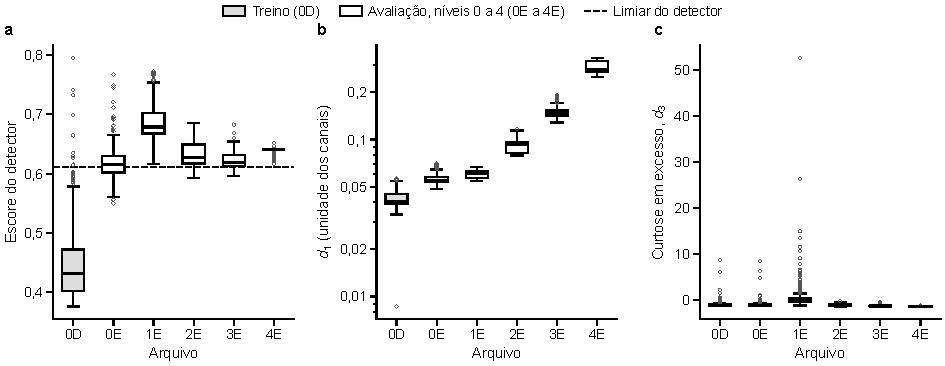
\includegraphics{fig_h4.pdf}
\fonte{elaborado pelo próprio autor, com dados de \citeonline{mey2022dados}.}
\legenda{distribuição, entre as janelas de cada arquivo da base pública, do escore do detector principal (\textbf{a}), de $d_1$ (\textbf{b}) e da curtose em excesso, $d_3$ (\textbf{c}). 0D é o arquivo de treino, e 0E a 4E, os de avaliação, com os níveis de desbalanceamento 0 a 4. A caixa vai do primeiro ao terceiro quartil, a linha interna marca a mediana, as hastes vão até 1,5 vez o intervalo interquartil, e os círculos são os valores além delas. Em \textbf{a}, a linha horizontal marca o limiar do detector, estimado no treino; em \textbf{b}, o eixo vertical está em escala logarítmica e na unidade dos canais, que a base não informa.}
\end{figure}

Com as sementes 0 a 9, previstas como descrição no registro de H4, o falso alarme em 0E variou de \hQuatroFaSementeMin~\% a \hQuatroFaSementeMax~\%, e a seção~\ref{sec:res-ap3} amplia essa variação para as sementes 0 a 99. A regra por mediana e MAD marcou \hQuatroFracaoMadZero~\% das janelas de 0E. Com a banda completa, o falso alarme foi de \hQuatroFracaoBandaCompletaZero~\%, e a fração marcada no nível 3 ficou em \hQuatroFracaoBandaCompletaTres~\%. Em nenhuma das variantes calculadas com a semente 0, o falso alarme ficou dentro dos \SI{10}{\percent} do critério de corroboração.

\section{Análises posteriores}\label{sec:res-posteriores}

Duas emendas ao registro acrescentaram seis análises posteriores, cada uma com o procedimento definido antes do cálculo (Apêndice~\ref{ap:registro}). A AP1 e a AP2, de 7 de novembro de 2026, examinam os resultados de H3 e de H2. A AP3 a AP6, de 8 de novembro, foram pedidas por pareceres sobre uma versão anterior deste texto e tratam da incerteza de H1, H2 e H4 e do escore do detector principal. Só a AP1 tem previsão registrada. As emendas mantiveram os critérios de H1 a H4, e as seis análises não alteram a avaliação dessas hipóteses.

\subsection{Assinatura em fase com a componente na rotação}\label{sec:res-ap1}

Em H3, a fase da assinatura foi sorteada em cada janela. Como o início da janela não é sincronizado com o eixo, a diferença de fase entre a assinatura e a componente na rotação já presente no sinal também variou ao acaso de uma janela para outra. Em um desbalanceamento real, a força acrescentada tem fase fixa em relação à do desbalanceamento existente, porque a massa fica em um ponto do rotor, e, com resposta linear da estrutura, essa diferença de fase é a mesma em todos os eixos. Na AP1, a componente na rotação já presente no sinal foi atribuída a desbalanceamento. Se parte dela tiver outra origem, como desalinhamento ou folga, a diferença de fase entre um desbalanceamento real e essa componente não será a mesma em todos os eixos.

A fase da componente na rotação de cada eixo radial foi medida em cada janela de teste, pelo coeficiente da transformada de Fourier da janela na frequência de rotação. A assinatura foi somada com diferença de fase $\theta$ de \SI{0}{\degree}, \SI{90}{\degree} ou \SI{180}{\degree} em relação a essa componente. As máquinas, a divisão entre treino e teste, o detector, o limiar e a grade de amplitudes foram os de H3, e a injeção foi conferida antes do cálculo em uma janela sintética com fase conhecida.

A previsão registrada era que, com $\theta = \SI{0}{\degree}$ e $A_v = \SI{2,8}{\milli\meter\per\second}$, o detector principal marcaria uma fração das janelas de teste maior que a de H3 na dobradeira, na calandra e no compressor, as três máquinas em que a mediana de $d_5$ passa de \SI{2,8}{\milli\meter\per\second}. A previsão não se confirmou, porque no compressor a fração com $\theta = \SI{0}{\degree}$ foi igual à de H3, de \apUmFracaoZeroCompressor~\% (Tabela~\ref{tab:ap1}). Na dobradeira, a fração passou de \apUmFracaoSorteadaDobradeira~\% em H3 para \apUmFracaoZeroDobradeira~\%, e na calandra, de \apUmFracaoSorteadaCalandra~\% para \apUmFracaoZeroCalandra~\%; sem assinatura, o detector já marcava \apUmFracaoSemAssinaturaCalandra~\% das janelas de teste da calandra. Em nenhuma máquina e com nenhum dos três valores de $\theta$, a fração marcada chegou a \SI{50}{\percent} até \SI{2,8}{\milli\meter\per\second} (Figura~\ref{fig:ap1}).

\begin{figure}[!htb]
\centering
\caption{Fração de janelas marcadas com a assinatura em fase fixa com a componente na rotação}\label{fig:ap1}
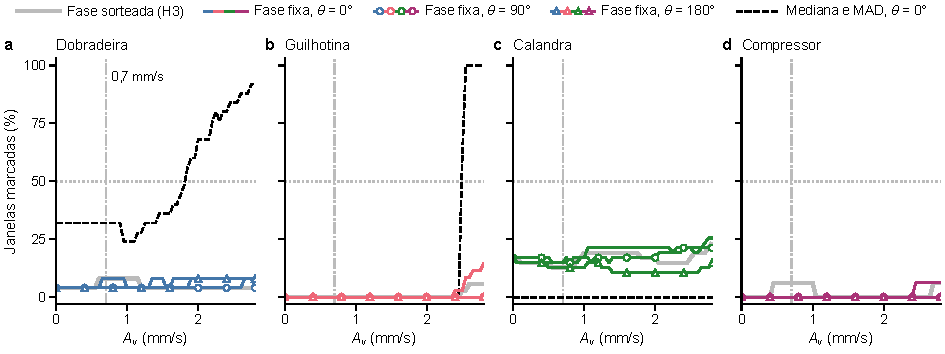
\includegraphics{fig_ap1.pdf}
\fonte{elaborado pelo próprio autor.}
\legenda{fração das janelas de teste marcadas em função da velocidade eficaz $A_v$ da assinatura na rotação, em cada eixo radial, na dobradeira (\textbf{a}), na guilhotina (\textbf{b}), na calandra (\textbf{c}) e no compressor (\textbf{d}). As séries de fase sorteada e de fase fixa são do detector principal. Com a fase sorteada, a de H3, a fase da assinatura variou ao acaso de uma janela para outra; com a fase fixa, $\theta$ é a diferença de fase em relação à componente na rotação de cada eixo. A linha horizontal marca os \SI{50}{\percent} que definem $A_{50}$, e a vertical, o tamanho de referência de \SI{0,7}{\milli\meter\per\second}.}
\end{figure}

\begin{table}[!htb]
\centering\small
\caption{Frações de janelas marcadas com a assinatura em fase fixa com a componente na rotação, na coleta de 2 de novembro de 2026}\label{tab:ap1}
\begin{tabular}{@{}llrrrrrrr@{}}
\toprule
Máquina & Base por eixo & \multicolumn{5}{c}{Detector principal (\%)} & $\Delta d_5$ & MAD \\
\cmidrule(lr){3-7}
 & (mm/s) & Sem & H3 & \SI{0}{\degree} & \SI{90}{\degree} & \SI{180}{\degree} & (mm/s) & (\%) \\
\midrule
Dobradeira & Y \apUmBaseDobradeiraY; Z \apUmBaseDobradeiraZ & \apUmFracaoSemAssinaturaDobradeira & \apUmFracaoSorteadaDobradeira & \apUmFracaoZeroDobradeira & \apUmFracaoNoventaDobradeira & \apUmFracaoCentoOitentaDobradeira & \apUmVariacaoDcincoZeroDobradeira & \apUmMadFracaoZeroDobradeira \\
Guilhotina & X \apUmBaseGuilhotinaX; Z \apUmBaseGuilhotinaZ & \apUmFracaoSemAssinaturaGuilhotina & \apUmFracaoSorteadaGuilhotina & \apUmFracaoZeroGuilhotina & \apUmFracaoNoventaGuilhotina & \apUmFracaoCentoOitentaGuilhotina & \apUmVariacaoDcincoZeroGuilhotina & \apUmMadFracaoZeroGuilhotina \\
Calandra & X \apUmBaseCalandraX; Z \apUmBaseCalandraZ & \apUmFracaoSemAssinaturaCalandra & \apUmFracaoSorteadaCalandra & \apUmFracaoZeroCalandra & \apUmFracaoNoventaCalandra & \apUmFracaoCentoOitentaCalandra & \apUmVariacaoDcincoZeroCalandra & \apUmMadFracaoZeroCalandra \\
Compressor & X \apUmBaseCompressorX; Z \apUmBaseCompressorZ & \apUmFracaoSemAssinaturaCompressor & \apUmFracaoSorteadaCompressor & \apUmFracaoZeroCompressor & \apUmFracaoNoventaCompressor & \apUmFracaoCentoOitentaCompressor & \apUmVariacaoDcincoZeroCompressor & \apUmMadFracaoZeroCompressor \\
\bottomrule
\end{tabular}
\fonte{elaborada pelo próprio autor.}
\nota{a base é a mediana da componente na rotação de cada eixo radial nas janelas de teste sem assinatura. A coluna Sem dá a fração marcada sem assinatura, e a coluna H3, a fração com a fase sorteada de H3; nas colunas \SI{0}{\degree}, \SI{90}{\degree} e \SI{180}{\degree}, $\theta$ é a diferença de fase entre a assinatura e a componente na rotação de cada eixo. $\Delta d_5$ é o aumento médio de $d_5$ nas janelas de teste, e MAD, a fração marcada pela regra por mediana e MAD, as duas com $\theta = \SI{0}{\degree}$. Exceto na coluna Sem, $A_v = \SI{2,8}{\milli\meter\per\second}$. O treino e o teste tiveram \apUmTreinoDobradeira\ e \apUmTesteDobradeira\ janelas na dobradeira, \apUmTreinoGuilhotina\ e \apUmTesteGuilhotina\ na guilhotina, \apUmTreinoCalandra\ e \apUmTesteCalandra\ na calandra e \apUmTreinoCompressor\ e \apUmTesteCompressor\ no compressor.}
\end{table}

Com $\theta = \SI{0}{\degree}$ e \SI{2,8}{\milli\meter\per\second}, a componente $d_5$ das janelas de teste aumentou em média de \apUmVariacaoDcincoZeroDobradeira~mm/s na dobradeira a \apUmVariacaoDcincoZeroGuilhotina~mm/s na guilhotina, enquanto a fração marcada pelo detector principal ficou entre \apUmFracaoZeroCompressor~\% e \apUmFracaoZeroCalandra~\%. Com a mesma injeção, a regra por mediana e MAD chegou a \SI{50}{\percent} de janelas marcadas com \apUmMadAcinquentaZeroDobradeira~mm/s na dobradeira e \apUmMadAcinquentaZeroGuilhotina~mm/s na guilhotina e, com \SI{2,8}{\milli\meter\per\second}, marcou \apUmMadFracaoZeroDobradeira~\% e \apUmMadFracaoZeroGuilhotina~\% das janelas de teste dessas máquinas. Sem assinatura, ela já marcava \apUmMadSemAssinaturaDobradeira~\% das janelas de teste da dobradeira. Na calandra e no compressor, a regra por mediana e MAD não marcou nenhuma janela com $\theta = \SI{0}{\degree}$.

Na dobradeira e na guilhotina, a mudança de $d_5$ produzida pela assinatura em fase bastou para a regra por mediana e MAD e não bastou para o detector principal, treinado com \apUmTreinoDobradeira\ e \apUmTreinoGuilhotina\ janelas. Na calandra e no compressor, nenhum dos dois detectores marcou a assinatura. Em H2, essas duas máquinas tiveram os três ensaios com menor mudança detectável acima de \SI{0,7}{\milli\meter\per\second}. Com a fase fixa, a fração marcada não chegou a \SI{50}{\percent} em nenhuma máquina, e a fase sorteada não explica a refutação de H3.

\subsection{Mediana de várias janelas por medição}\label{sec:res-ap2}

Em H2, cada medição foi uma janela de \SI{0,512}{\second}. Na AP2, a medição passou a ser a mediana de $d_1$ em $k$ janelas consecutivas, com $k$ de 1 a 5, e a menor mudança detectável foi calculada sobre essas medianas como em H2, nos cinco ensaios do critério (Tabela~\ref{tab:ap2}). Janelas consecutivas estavam separadas por \campoCicloUm~s na primeira rodada e por \campoCicloDois~s na segunda, de modo que a mediana de cinco janelas reúne medições espalhadas por quatro desses intervalos. A AP2 não indica o que aconteceria com janelas adquiridas sem intervalo entre elas.

Nos três ensaios em que a menor mudança detectável de uma janela passou de \SI{0,7}{\milli\meter\per\second}, a mediana de até cinco janelas não a levou abaixo desse valor. Nas duas rodadas da calandra, ela diminuiu de \apDoisMmdCalandraUmUm\ e \apDoisMmdCalandraDoisUm~mm/s com uma janela para \apDoisMmdCalandraUmCinco\ e \apDoisMmdCalandraDoisCinco~mm/s com cinco, e no compressor aumentou de \apDoisMmdCompressorUmUm\ para \apDoisMmdCompressorUmCinco~mm/s. Na dobradeira e na segunda rodada da guilhotina, que já ficavam abaixo de \SI{0,7}{\milli\meter\per\second} com uma janela, a menor mudança detectável com cinco janelas foi de \apDoisMmdDobradeiraUmCinco\ e \apDoisMmdGuilhotinaDoisCinco~mm/s.

\begin{table}[!htb]
\centering\small
\caption{Menor mudança detectável no descritor $d_1$ com a mediana de $k$ janelas por medição, na coleta de 2 de novembro de 2026}\label{tab:ap2}
\begin{tabular}{@{}llrrrrrrr@{}}
\toprule
Máquina & Rodada & Janelas & \multicolumn{5}{c}{Menor mudança detectável (mm/s)} & Autocorrelação \\
\cmidrule(lr){4-8}
 & & & $k = 1$ & $k = 2$ & $k = 3$ & $k = 4$ & $k = 5$ & \\
\midrule
Dobradeira & 1 & \hDoisNDobradeiraUm & \apDoisMmdDobradeiraUmUm & \apDoisMmdDobradeiraUmDois & \apDoisMmdDobradeiraUmTres & \apDoisMmdDobradeiraUmQuatro & \apDoisMmdDobradeiraUmCinco & \apDoisAutocorrDobradeiraUm \\
Guilhotina & 2 & \hDoisNGuilhotinaDois & \apDoisMmdGuilhotinaDoisUm & \apDoisMmdGuilhotinaDoisDois & \apDoisMmdGuilhotinaDoisTres & \apDoisMmdGuilhotinaDoisQuatro & \apDoisMmdGuilhotinaDoisCinco & \apDoisAutocorrGuilhotinaDois \\
Calandra & 1 & \hDoisNCalandraUm & \apDoisMmdCalandraUmUm & \apDoisMmdCalandraUmDois & \apDoisMmdCalandraUmTres & \apDoisMmdCalandraUmQuatro & \apDoisMmdCalandraUmCinco & \apDoisAutocorrCalandraUm \\
Calandra & 2 & \hDoisNCalandraDois & \apDoisMmdCalandraDoisUm & \apDoisMmdCalandraDoisDois & \apDoisMmdCalandraDoisTres & \apDoisMmdCalandraDoisQuatro & \apDoisMmdCalandraDoisCinco & \apDoisAutocorrCalandraDois \\
Compressor & 1 & \hDoisNCompressorUm & \apDoisMmdCompressorUmUm & \apDoisMmdCompressorUmDois & \apDoisMmdCompressorUmTres & \apDoisMmdCompressorUmQuatro & \apDoisMmdCompressorUmCinco & \apDoisAutocorrCompressorUm \\
\bottomrule
\end{tabular}
\fonte{elaborada pelo próprio autor.}
\nota{com $k$ janelas, a medição é a mediana móvel de $d_1$ em $k$ janelas consecutivas, com passo de uma janela, e a menor mudança detectável é calculada sobre essas medianas como em H2; com $k = 1$, ela é a da Tabela~\ref{tab:h2}. A autocorrelação é a correlação de Pearson entre os valores de $d_1$ de janelas consecutivas.}
\end{table}

O compressor foi o único ensaio com autocorrelação positiva de $d_1$ entre janelas consecutivas, de \apDoisAutocorrCompressorUm. Com autocorrelação positiva, janelas vizinhas variam juntas, e a mediana delas reduz pouco a variação, o que é compatível com o aumento da menor mudança detectável no compressor. Nos outros quatro ensaios, a autocorrelação foi de \apDoisAutocorrDobradeiraUm\ a \apDoisAutocorrGuilhotinaDois.

Em dois ensaios, a menor mudança detectável não diminuiu de forma monotônica com $k$. Na segunda rodada da guilhotina, ela aumentou para \apDoisMmdGuilhotinaDoisDois~mm/s com duas janelas e diminuiu para \apDoisMmdGuilhotinaDoisTres~mm/s com três. A mediana de duas janelas é a média delas e mantém metade de um valor alto isolado, que a de três janelas descarta, e essa diminuição é compatível com valores altos em janelas isoladas. Na segunda rodada da calandra, a menor mudança detectável oscilou entre \apDoisMmdCalandraDoisQuatro\ e \apDoisMmdCalandraDoisTres~mm/s de $k = 2$ a $k = 5$. Como medianas vizinhas compartilham janelas, o quantil de \SI{95}{\percent} da série depende de poucos valores altos.

\subsection{Falso alarme com outras sementes e com o treino reamostrado}\label{sec:res-ap3}

O limiar e o modelo de H1 e de H4 foram estimados uma vez, com a semente 0 do gerador de números aleatórios do Isolation Forest, e o intervalo registrado reamostra só as janelas de teste. A AP3 mediu a variação que esse intervalo não inclui de duas formas. Na primeira, o detector foi treinado com as sementes de 0 a \num{99}, cada uma com o seu limiar, sobre o mesmo treino e o mesmo teste. Na segunda, em \apTresReplicas\ réplicas, o treino foi reamostrado por blocos de cinco janelas consecutivas, e o limiar e o modelo foram refeitos com uma semente diferente em cada réplica, antes da reamostragem do teste. Na validação do limiar, todas as cópias de um mesmo bloco ficaram no mesmo grupo, para que nenhuma janela recebesse escore de um modelo treinado com ela. Na calandra, \apTresDescartesCalandra\ das \apTresReplicas\ réplicas teve um só bloco distinto no treino, sem como validar o limiar, e foi descartada, caso que o registro não previa. A segunda forma não se aplica à guilhotina, cujo treino de \campoJanelasGuilhotinaUm\ janelas tem só três blocos.

Na calandra, a fração marcada na segunda rodada teve mediana de \apTresSementeCalandraMed~\% entre as \apTresSementes\ sementes, com \SI{95}{\percent} delas de \apTresSementeCalandraPInf~\% a \apTresSementeCalandraPSup~\% e extremos de \apTresSementeCalandraMin~\% e \apTresSementeCalandraMax~\% (Tabela~\ref{tab:ap3}). A semente 0, registrada, deu \hUmFracaoCalandra~\%, acima da mediana. A fração ficou em até \SI{10}{\percent} com \apTresSementeCalandraAteDez\ sementes e passou de \SI{20}{\percent} com \apTresSementeCalandraAcimaVinte. Com o treino reamostrado, o intervalo foi de \apTresTreinoInfCalandra~\% a \apTresTreinoSupCalandra~\%, mais largo que o registrado, de \hUmCalandraIFDiretoInf~\% a \hUmCalandraIFDiretoSup~\%. Na guilhotina, nenhuma das \apTresSementes\ florestas, treinadas com as \campoJanelasGuilhotinaUm\ janelas da primeira rodada, marcou janela da segunda.

Pelos critérios registrados, aplicados a cada semente com o intervalo do teste reamostrado, H1 seria corroborada com \apTresVereditoUmCorroborada\ sementes, indeterminada com \apTresVereditoUmIndeterminada\ e refutada com \apTresVereditoUmRefutada. O veredito de H1 depende, portanto, da semente do detector, e o veredito registrado, calculado com a semente 0, continua valendo.

Em H4, o falso alarme em 0E teve mediana de \apTresSementeNivelZeroMed~\% entre as sementes, com \SI{95}{\percent} delas de \apTresSementeNivelZeroPInf~\% a \apTresSementeNivelZeroPSup~\%. O número de sementes com falso alarme acima de \SI{20}{\percent} foi \apTresSementeNivelZeroAcimaVinte, e o de sementes com até \SI{10}{\percent}, \apTresSementeNivelZeroAteDez. A fração marcada chegou a \SI{50}{\percent} nos quatro níveis de desbalanceamento ao mesmo tempo com \apTresSementeNiveisCinquenta\ sementes. Com o treino reamostrado, o intervalo do falso alarme foi de \apTresTreinoInfNivelZero~\% a \apTresTreinoSupNivelZero~\%. Pelos critérios registrados, H4 seria refutada com \apTresVereditoQuatroRefutada\ sementes e indeterminada com \apTresVereditoQuatroIndeterminada, e o número de sementes que a corroborariam foi \apTresVereditoQuatroCorroborada. A refutação de H4 não depende, portanto, da semente.

Com o treino reamostrado, a fração marcada nos níveis 2 a 4 também foi de quase nenhuma janela a todas, e em \descReplicasSemMarcacaoQuatro\ das \apTresReplicas\ réplicas nenhuma janela de 4E, o nível de maior desbalanceamento, passou do limiar. Para descrever esse resultado, o modelo registrado de H4 foi aplicado de novo às janelas de cada arquivo, numa descrição acrescentada depois do cálculo e fora do registro. As janelas de 4E tinham, em mediana, \descForaMedianaQuatro\ descritores fora da faixa do treino, e o escore delas ficou entre \descEscoreCincoPctQuatro, no percentil de \SI{5}{\percent}, e \descEscoreMaxQuatro, no máximo, pouco acima do limiar registrado, de \descLimiarQuatro. O escore das janelas de maior desbalanceamento ficou, assim, numa faixa estreita, compatível com o teto do escore fora da faixa do treino (seção~\ref{sec:res-ap6}). Com outro treino e outro limiar, essa faixa pode ficar toda abaixo do limiar, como nas réplicas sem nenhuma janela marcada.

\begin{table}[!htb]
\centering\small
\caption{Fração de janelas marcadas com as sementes de 0 a 99 e com o treino reamostrado}\label{tab:ap3}
\setlength{\tabcolsep}{4pt}
\begin{tabular}{@{}llrrrrr@{}}
\toprule
Hipótese & Teste & Semente 0 & \multicolumn{3}{c}{Sementes de 0 a \num{99} (\%)} & Treino \\
\cmidrule(lr){4-6}
 & & (\%) & Mediana & \SI{95}{\percent} das sementes & Extremos & reamostrado (\%) \\
\midrule
H1, calandra & rodada 2 & \hUmFracaoCalandra & \apTresSementeCalandraMed & \apTresSementeCalandraPInf\ a \apTresSementeCalandraPSup & \apTresSementeCalandraMin\ a \apTresSementeCalandraMax & \apTresTreinoInfCalandra\ a \apTresTreinoSupCalandra \\
H1, guilhotina & rodada 2 & \hUmFracaoGuilhotina & \apTresSementeGuilhotinaMed & \apTresSementeGuilhotinaPInf\ a \apTresSementeGuilhotinaPSup & \apTresSementeGuilhotinaMin\ a \apTresSementeGuilhotinaMax & \\
H4 & 0E & \hQuatroFracaoZero & \apTresSementeNivelZeroMed & \apTresSementeNivelZeroPInf\ a \apTresSementeNivelZeroPSup & \apTresSementeNivelZeroMin\ a \apTresSementeNivelZeroMax & \apTresTreinoInfNivelZero\ a \apTresTreinoSupNivelZero \\
H4 & 1E & \hQuatroFracaoUm & \apTresSementeNivelUmMed & \apTresSementeNivelUmPInf\ a \apTresSementeNivelUmPSup & \apTresSementeNivelUmMin\ a \apTresSementeNivelUmMax & \apTresTreinoInfNivelUm\ a \apTresTreinoSupNivelUm \\
H4 & 2E & \hQuatroFracaoDois & \apTresSementeNivelDoisMed & \apTresSementeNivelDoisPInf\ a \apTresSementeNivelDoisPSup & \apTresSementeNivelDoisMin\ a \apTresSementeNivelDoisMax & \apTresTreinoInfNivelDois\ a \apTresTreinoSupNivelDois \\
H4 & 3E & \hQuatroFracaoTres & \apTresSementeNivelTresMed & \apTresSementeNivelTresPInf\ a \apTresSementeNivelTresPSup & \apTresSementeNivelTresMin\ a \apTresSementeNivelTresMax & \apTresTreinoInfNivelTres\ a \apTresTreinoSupNivelTres \\
H4 & 4E & \hQuatroFracaoQuatro & \apTresSementeNivelQuatroMed & \apTresSementeNivelQuatroPInf\ a \apTresSementeNivelQuatroPSup & \apTresSementeNivelQuatroMin\ a \apTresSementeNivelQuatroMax & \apTresTreinoInfNivelQuatro\ a \apTresTreinoSupNivelQuatro \\
\bottomrule
\end{tabular}
\fonte{elaborada pelo próprio autor, com dados de \citeonline{mey2022dados} nas linhas de H4.}
\nota{semente 0: valor registrado. Nas sementes de 0 a \num{99}, cada floresta tem o seu limiar, com o mesmo treino e o mesmo teste; \SI{95}{\percent} das sementes vai do percentil de \SI{2,5}{\percent} ao de \SI{97,5}{\percent}. Treino reamostrado: intervalo de \SI{95}{\percent} de \apTresReplicas\ réplicas, com treino e teste reamostrados por blocos e limiar e modelo refeitos em cada réplica; não calculado na guilhotina, cujo treino tem três blocos. Em H1, o teste é a segunda rodada; em H4, 0E não tem desbalanceamento, e 1E a 4E têm os níveis 1 a 4.}
\end{table}

\subsection{Intervalo da menor mudança detectável}\label{sec:res-ap4}

A menor mudança detectável de H2 é a diferença entre o quantil de \SI{95}{\percent} e a mediana de $d_1$, e o quantil de \SI{95}{\percent} de \num{25} a \num{50} janelas depende das duas ou três janelas mais altas. Na AP4, as janelas de cada ensaio foram reamostradas por blocos de cinco janelas consecutivas, em \num{2000} réplicas, e a menor mudança detectável foi recalculada em cada réplica (Tabela~\ref{tab:ap4}).

\begin{table}[!htb]
\centering\small
\caption{Intervalo da menor mudança detectável no descritor $d_1$ e comparação com o sensor em repouso, na coleta de 2 de novembro de 2026}\label{tab:ap4}
\setlength{\tabcolsep}{4pt}
\begin{tabular}{@{}llrrrr@{}}
\toprule
Ensaio & Rodada & \multicolumn{2}{c}{Menor mudança detectável (mm/s)} & Réplicas acima & Razão com \\
\cmidrule(lr){3-4}
 & & Amostra & Intervalo de \SI{95}{\percent} & de \SI{0,7}{\milli\meter\per\second} (\%) & o repouso \\
\midrule
Dobradeira & 1 & \hDoisMmdDobradeiraUm & \apQuatroInfDobradeiraUm\ a \apQuatroSupDobradeiraUm & \apQuatroAcimaDobradeiraUm & \apCincoRazaoDobradeiraUm \\
Guilhotina & 1 & \hDoisMmdGuilhotinaUm & \apQuatroInfGuilhotinaUm\ a \apQuatroSupGuilhotinaUm & \apQuatroAcimaGuilhotinaUm & \\
Guilhotina & 2 & \hDoisMmdGuilhotinaDois & \apQuatroInfGuilhotinaDois\ a \apQuatroSupGuilhotinaDois & \apQuatroAcimaGuilhotinaDois & \apCincoRazaoGuilhotinaDois \\
Calandra & 1 & \hDoisMmdCalandraUm & \apQuatroInfCalandraUm\ a \apQuatroSupCalandraUm & \apQuatroAcimaCalandraUm & \apCincoRazaoCalandraUm \\
Calandra & 2 & \hDoisMmdCalandraDois & \apQuatroInfCalandraDois\ a \apQuatroSupCalandraDois & \apQuatroAcimaCalandraDois & \apCincoRazaoCalandraDois \\
Compressor & 1 & \hDoisMmdCompressorUm & \apQuatroInfCompressorUm\ a \apQuatroSupCompressorUm & \apQuatroAcimaCompressorUm & \apCincoRazaoCompressorUm \\
\midrule
Repouso & & \apCincoMmd & \apCincoMmdInf\ a \apCincoMmdSup & & \\
Repouso, X e Y & & \apCincoMmdHorizontal & \apCincoMmdInfHorizontal\ a \apCincoMmdSupHorizontal & & \\
\bottomrule
\end{tabular}
\fonte{elaborada pelo próprio autor.}
\nota{intervalo pelos percentis de \SI{2,5}{\percent} e \SI{97,5}{\percent} de \num{2000} réplicas, com reamostragem por blocos de cinco janelas consecutivas. A razão com o repouso divide a menor mudança detectável do ensaio pela do sensor em repouso, de \apCincoMmd~mm/s, calculada pela mesma regra nas \apCincoJanelas\ janelas com o transmissor sobre a mesa; a primeira rodada da guilhotina, fora do critério de H2, não tem razão calculada. Na linha Repouso, X e Y, $d_1$ é o maior valor entre os eixos horizontais X e Y.}
\end{table}

Nas duas rodadas da calandra e no compressor, todas as réplicas ficaram acima de \SI{0,7}{\milli\meter\per\second}, e o limite inferior do intervalo foi de \apQuatroInfCompressorUm~mm/s no compressor a \apQuatroInfCalandraDois~mm/s na segunda rodada da calandra. Na dobradeira, nenhuma réplica chegou a \SI{0,7}{\milli\meter\per\second}, e o intervalo foi de \apQuatroInfDobradeiraUm\ a \apQuatroSupDobradeiraUm~mm/s. Na segunda rodada da guilhotina, o intervalo foi de \apQuatroInfGuilhotinaDois\ a \apQuatroSupGuilhotinaDois~mm/s, e \apQuatroAcimaGuilhotinaDois~\% das réplicas passaram de \SI{0,7}{\milli\meter\per\second}. A largura desse intervalo se deve a poucas janelas com $d_1$ alto, que entram em parte das réplicas e ficam fora de outras. Com amostras desse tamanho, a reamostragem de quantis extremos tende a dar intervalos estreitos demais, e os intervalos da Tabela~\ref{tab:ap4} são aproximados.

\subsection{Menor mudança detectável com o sensor em repouso}\label{sec:res-ap5}

A comparação com o ruído usa, na AP5, a mesma regra de H2 aplicada às \apCincoJanelas\ janelas com o transmissor parado sobre a mesa. Nessas janelas, a mediana de $d_1$ foi de \apCincoMediana~mm/s, e a menor mudança detectável, de \apCincoMmd~mm/s, com intervalo de \apCincoMmdInf\ a \apCincoMmdSup~mm/s (Tabela~\ref{tab:ap4}). Só com os eixos horizontais, X e Y, sem o eixo vertical, que tem linhas compatíveis com a vibração da mesa (seção~\ref{sec:res-aquisicao}), a menor mudança detectável em repouso foi de \apCincoMmdHorizontal~mm/s.

Nos cinco ensaios do critério de H2, a menor mudança detectável ficou de \apCincoRazaoMin\ a \apCincoRazaoMax\ vezes a do repouso, e de \apCincoRazaoHorizontalMin\ a \apCincoRazaoHorizontalMax\ vezes a do repouso só nos eixos horizontais. As duas razões passam de 1 em todos os ensaios, e a variação de $d_1$ entre janelas nas máquinas foi maior que a do mesmo descritor com o sensor parado. A razão não separa a máquina da fixação, porque o sinal das máquinas inclui as duas e o do repouso não inclui nenhuma.

\subsection{Escore do detector fora da faixa do treino}\label{sec:res-ap6}

Em cada árvore do Isolation Forest, o valor da divisão de um nó é sorteado entre o mínimo e o máximo das janelas desse nó. Uma janela além do máximo do treino num descritor segue o mesmo caminho em qualquer distância além dele, e o escore deixa de crescer com a distância. Na AP6, o escore foi calculado em pontos sintéticos com a mediana do treino em cada descritor, exceto nos descritores deslocados para além da faixa do treino, e comparado com o limiar de cada modelo (Tabela~\ref{tab:ap6}). Antes do cálculo, o escore de cada ponto foi conferido com o dobro da distância além da faixa, e não mudou.

\begin{table}[!htb]
\centering\small
\caption{Escore do detector principal em pontos fora da faixa do treino}\label{tab:ap6}
\begin{tabular}{@{}lrrrrrr@{}}
\toprule
Modelo & Treino & Limiar & Referência & Um descritor & $d_1$, $d_2$ e $d_5$ & Seis descritores \\
 & (janelas) & & & fora (maior) & fora & fora \\
\midrule
Dobradeira & \apSeisTreinoDobradeira & \apSeisLimiarDobradeira & \apSeisReferenciaDobradeira & \apSeisUmMaxDobradeira & \apSeisTresDobradeira & \apSeisTodosDobradeira \\
Guilhotina & \apSeisTreinoGuilhotina & \apSeisLimiarGuilhotina & \apSeisReferenciaGuilhotina & \apSeisUmMaxGuilhotina & \apSeisTresGuilhotina & \apSeisTodosGuilhotina \\
Calandra & \apSeisTreinoCalandra & \apSeisLimiarCalandra & \apSeisReferenciaCalandra & \apSeisUmMaxCalandra & \apSeisTresCalandra & \apSeisTodosCalandra \\
Compressor & \apSeisTreinoCompressor & \apSeisLimiarCompressor & \apSeisReferenciaCompressor & \apSeisUmMaxCompressor & \apSeisTresCompressor & \apSeisTodosCompressor \\
Base pública & \hQuatroNTreino & \apSeisLimiarQuatro & \apSeisReferenciaQuatro & \apSeisUmMaxQuatro & \apSeisTresQuatro & \apSeisTodosQuatro \\
\bottomrule
\end{tabular}
\fonte{elaborada pelo próprio autor, com dados de \citeonline{mey2022dados} na última linha.}
\nota{escore do detector principal com a semente 0, nos modelos de H3 (os da guilhotina e da calandra são também os de H1) e no de H4. Referência: ponto com a mediana do treino nos seis descritores. Fora: descritor colocado além do máximo do treino, ou abaixo do mínimo na coluna de um descritor, que dá o maior escore entre os doze pontos com um só descritor deslocado. Os demais descritores ficam na mediana do treino.}
\end{table}

Com um só descritor fora da faixa, o escore ficou abaixo do limiar nos cinco modelos, em qualquer direção e em qualquer distância. Com $d_1$, $d_2$ e $d_5$ fora da faixa, os três descritores que a assinatura de H3 aumenta, o escore passou do limiar só no modelo da dobradeira, com \apSeisTresDobradeira\ contra \apSeisLimiarDobradeira, e ficou abaixo dele nos modelos da guilhotina, da calandra, do compressor e da base pública. Nesses quatro modelos, uma janela que mude só esses três descritores, com os demais perto da mediana do treino, não alcança o limiar em nenhuma amplitude. Com os seis descritores fora, o escore passou do limiar em todos os modelos.

Na injeção de H3, a mediana de $d_5$ das janelas de teste passou do máximo do treino com \apSeisAsatGuilhotina~mm/s na guilhotina, \apSeisAsatDobradeira~mm/s na dobradeira e \apSeisAsatCompressor~mm/s no compressor, e na calandra não passou até \SI{2,8}{\milli\meter\per\second}. Com \SI{2,8}{\milli\meter\per\second}, \apSeisJanelasDcincoAcimaGuilhotina\ das \apSeisTesteGuilhotina\ janelas de teste da guilhotina estavam com $d_5$ acima do máximo do treino, e a mediana do escore foi de \apSeisEscoreAltoGuilhotina, abaixo do limiar de \apSeisLimiarGuilhotina. Pela leitura registrada, a refutação de H3 na guilhotina e no compressor se deve ao escore máximo do detector com o treino de cada máquina, e não à amplitude da assinatura. Na calandra, o escore máximo com os três descritores fora também fica abaixo do limiar, mas a assinatura de \SI{2,8}{\milli\meter\per\second} não chegou a levar a mediana de $d_5$ além da faixa do treino, porque a componente já presente tinha mediana de \hTresBaseUmXCalandra~mm/s.

\chapter{Discussão}\label{cap:discussao}

Os resultados não sustentam a hipótese central. Com a linha de base de uma rodada, o detector principal marcou parte da operação normal medida depois de mudanças na montagem e não marcou assinaturas de desbalanceamento do tamanho que a norma considera significativo. A menor mudança detectável em $d_1$ passou de \SI{0,7}{\milli\meter\per\second} em três dos cinco ensaios avaliados, e, na base pública, depois da remontagem do suporte, o detector marcou \hQuatroFracaoZero~\% das janelas sem desbalanceamento. As análises posteriores mostraram dois limites do próprio detector. O falso alarme estimado com poucas janelas de treino variou com a semente do gerador de números aleatórios, a ponto de H1 ser corroborada com parte das sementes, e o escore do Isolation Forest tem um teto que impediu a marcação da assinatura em três das quatro máquinas. A cadeia de aquisição entregou completas todas as janelas dos trechos analisados, e as perdas do enlace ficaram fora deles (seção~\ref{sec:disc-sistema}).

\section{Falso alarme e estabilidade da linha de base}\label{sec:disc-falso-alarme}

O detector principal marcou operação normal medida depois de mudanças na montagem. Na calandra, treinado na primeira rodada, ele marcou \hUmCalandraIFDireto~\% das janelas da segunda, com intervalo de \hUmCalandraIFDiretoInf~\% a \hUmCalandraIFDiretoSup~\% (seção~\ref{sec:res-h1}). Entre as rodadas, mudaram ao mesmo tempo a fixação, a alimentação, o intervalo entre ciclos e a temperatura do sensor, de \campoTempCalandraUm\ para \campoTempCalandraDois~\si{\celsius}, e os dados não indicam qual dessas mudanças produziu a marcação. Na base pública, o falso alarme em 0E foi de \hQuatroFracaoZero~\%, depois da remontagem do suporte do desbalanceamento, e, de 0D para 0E, a mediana de $d_1$ passou de \hQuatroDumMedianaTreino\ para \hQuatroDumMedianaZero\ na unidade dos canais (seção~\ref{sec:res-h4}). Nos dois casos, o treino e o teste foram medidos na mesma máquina sem falha, em montagens diferentes, e o detector não distingue essa diferença de uma falha.

Com poucas janelas de treino, o falso alarme estimado dependeu da semente do detector e do próprio treino. Na calandra, com as sementes de 0 a \num{99}, a fração marcada teve mediana de \apTresSementeCalandraMed~\%, abaixo dos \hUmCalandraIFDireto~\% da semente registrada, e H1 seria corroborada com \apTresVereditoUmCorroborada\ das \apTresSementes\ sementes (seção~\ref{sec:res-ap3}). Com o treino reamostrado e o limiar refeito, o intervalo da calandra foi de \apTresTreinoInfCalandra~\% a \apTresTreinoSupCalandra~\%. Na base pública, com \hQuatroNTreino\ janelas de treino, \SI{95}{\percent} das sementes deram falso alarme em 0E de \apTresSementeNivelZeroPInf~\% a \apTresSementeNivelZeroPSup~\%. Na análise de valores discrepantes, o limiar depende do número de observações e do número de dimensões \cite[p.~650]{worden2000}, e o limiar deste trabalho foi estimado com \campoJanelasGuilhotinaUm\ a \campoJanelasCalandraUm\ janelas e seis descritores. O veredito indeterminado de H1 reflete, portanto, a variação do próprio detector treinado com \campoJanelasCalandraUm\ janelas, além do falso alarme entre rodadas, e uma estimativa que varia de \apTresTreinoInfCalandra~\% a \apTresTreinoSupCalandra~\% não permite fixar um limiar de operação.

Na guilhotina, o falso alarme de \hUmGuilhotinaIFDireto~\% se repetiu com as \apTresSementes\ sementes, e o mesmo modelo marcou \condGuilhotinaParado~\% das janelas com o motor desligado (seção~\ref{sec:res-condicao}). Com \campoJanelasGuilhotinaUm\ janelas de treino, o detector da guilhotina quase não marca janela alguma, e o falso alarme nulo não mede a estabilidade da linha de base dessa máquina.

O escore do Isolation Forest tem um teto fora da faixa do treino. Em cada nó de uma árvore, o valor da divisão é sorteado entre o mínimo e o máximo das amostras de treino que chegam ao nó \cite{liu2008}, e uma janela além do valor extremo do treino percorre o mesmo caminho em qualquer distância além dele. Na AP6, com $d_1$, $d_2$ e $d_5$ além da faixa do treino e os demais descritores na mediana, o escore ficou abaixo do limiar nos modelos da guilhotina, da calandra, do compressor e da base pública, e com os seis descritores fora passou dele em todos os modelos (seção~\ref{sec:res-ap6}). O detector marca uma janela que se afasta do treino em vários descritores ao mesmo tempo e não marca uma mudança restrita aos descritores que a assinatura de desbalanceamento altera, por maior que ela seja. Na base pública, as janelas de 4E tinham, em mediana, os seis descritores fora da faixa, e o escore delas ficou entre \descEscoreCincoPctQuatro\ e \descEscoreMaxQuatro, logo acima do limiar de \descLimiarQuatro. Com outro treino, nenhuma delas foi marcada em \descReplicasSemMarcacaoQuatro\ das \apTresReplicas\ réplicas (seção~\ref{sec:res-ap3}).

O treino de cada máquina teve de \campoJanelasGuilhotinaUm\ a \campoJanelasCalandraUm\ janelas de um mesmo ensaio, uma a cada \campoCicloUm~s, e não cobriu a variação ao longo de semanas, com carga, temperatura e nova fixação do sensor. O falso alarme ocorreu entre rodadas da mesma máquina separadas por \campoIntervaloCalandra\ e entre duas montagens da mesma bancada. Em laboratório, \citeonline[p.~330--331]{manson2000} observaram resultado semelhante. Com a condição normal de um período curto, os dados de uma estrutura sem dano passaram do limiar quando a temperatura da sala subiu de \SI{20}{\celsius} para \SI{31}{\celsius}. Pelo axioma IVb de \citeonline[p.~1640]{worden2007}, sem uma extração de descritores feita para isso, uma medida mais sensível ao dano é também mais sensível às mudanças das condições de operação e de ambiente. Os resultados indicam que a linha de base deve incluir mais de uma condição de montagem, e os dados não indicam quantas rodadas ou quais condições bastariam.

\section{Sensibilidade diante do critério da norma}\label{sec:disc-sensibilidade}

A menor mudança detectável dependeu da variação de $d_1$ entre janelas do sinal medido, que reúne a vibração da máquina e a resposta da fixação do transmissor. Pela mesma regra, ela ficou de \apCincoRazaoMin\ a \apCincoRazaoMax\ vezes a do sensor em repouso, de \apCincoMmd~mm/s (seção~\ref{sec:res-ap5}). Se a variação do repouso e a das máquinas forem independentes, elas se somam em quadratura, e, mesmo no ensaio com a menor razão, eliminar toda a variação do repouso reduziria a menor mudança detectável em cerca de \SI{5}{\percent}. Um sensor com menos ruído teria, portanto, pouco efeito sobre a menor mudança detectável desses ensaios, e o que resta da variação é da máquina e da fixação, que os dados não separam.

A comparação com \SI{0,7}{\milli\meter\per\second} supõe que a fixação transmite a vibração da carcaça sem ganho nem atenuação, o que não foi verificado. A menor mudança detectável relativa à mediana de $d_1$, de \hDoisRelDobradeiraUm~\% na dobradeira a \hDoisRelGuilhotinaDois~\% na segunda rodada da guilhotina (Tabela~\ref{tab:h2}), não depende de um ganho constante da fixação, porque esse ganho multiplica a mediana e o quantil pelo mesmo fator. Em valor absoluto, a menor mudança detectável da segunda rodada da calandra só ficaria abaixo de \SI{0,7}{\milli\meter\per\second} na carcaça com um ganho da fixação maior que \num{4,6}, razão entre \hDoisMmdCalandraDois\ e \SI{0,7}{\milli\meter\per\second}. As decisões de H2 e H3 também se mantêm para qualquer referência de mudança até \SI{2,8}{\milli\meter\per\second}, porque a menor mudança detectável da segunda rodada da calandra passou desse valor e nenhuma máquina chegou a \SI{50}{\percent} de janelas marcadas até ele. A referência de \SI{0,7}{\milli\meter\per\second} foi derivada do critério de mudança da série ISO 10816 descrito por \citeonline{schwirzer2002}, e o texto da ISO 20816-3 não foi conferido (seção~\ref{sec:hipoteses}).

A mediana de várias janelas por medição não levou a menor mudança detectável abaixo de \SI{0,7}{\milli\meter\per\second} nos ensaios com mais variação. Com até cinco janelas, cobrindo cerca de um minuto, ela continuou acima desse valor na calandra e no compressor (seção~\ref{sec:res-ap2}). No compressor, a autocorrelação de \apDoisAutocorrCompressorUm\ entre janelas consecutivas indica uma variação lenta, que uma mediana de janelas vizinhas reduz pouco. A reamostragem da AP4 manteve esse quadro, com todas as réplicas da calandra e do compressor acima de \SI{0,7}{\milli\meter\per\second} e as da dobradeira abaixo (seção~\ref{sec:res-ap4}). Na segunda rodada da guilhotina, \apQuatroAcimaGuilhotinaDois~\% das réplicas passaram desse valor, e a posição dela em relação ao critério é incerta. Separar a variação lenta de uma falha exigiria conhecer as condições de que ela depende, como a carga ou o ciclo de trabalho, que a coleta não registrou.

Nenhum detector marcou metade das janelas com uma assinatura de \SI{0,7}{\milli\meter\per\second}. Com a fase sorteada de H3, o detector principal não chegou a \SI{50}{\percent} até \SI{2,8}{\milli\meter\per\second}, quatro vezes o critério, e com a fase fixa da AP1 também não (seção~\ref{sec:res-ap1}). Na guilhotina e no compressor, a assinatura levou $d_5$ além da faixa do treino, e o escore máximo com os descritores que ela altera ficou abaixo do limiar, de modo que o limite está no escore do detector (seção~\ref{sec:res-ap6}). Na calandra, a componente na rotação já presente, com mediana de \hTresBaseUmXCalandra~mm/s, fez a assinatura mudar pouco $d_5$. Na dobradeira, o ponto com os três descritores fora da faixa passa do limiar, mas a assinatura de \SI{2,8}{\milli\meter\per\second} levou $d_5$ além da faixa em \apSeisJanelasDcincoAcimaDobradeira\ das \hTresTesteDobradeira\ janelas de teste. A regra por mediana e MAD, que avalia cada descritor separadamente, chegou a \SI{50}{\percent} com a fase fixa na dobradeira, com \apUmMadAcinquentaZeroDobradeira~mm/s, e na guilhotina, com \apUmMadAcinquentaZeroGuilhotina~mm/s.

As medianas axiais de \SIrange{10}{184}{\hertz} da dobradeira, da calandra e do compressor ficaram acima do limite entre as zonas C e D do grupo 2 em fundação rígida, e a direção axial teve a maior velocidade nessas três máquinas (seção~\ref{sec:res-base}). O operador, porém, descreveu as três máquinas como saudáveis. Os dados não separam quatro explicações: a resposta da fixação, com fita dupla face, invólucro e espumas entre a carcaça e o sensor (seção~\ref{sec:ensaios}); o ponto de medição na carcaça do motor; a massa do transmissor; ou máquinas de fato fora da zona B. Nenhuma delas pode ser descartada sem um sensor de referência no mesmo ponto.

\section{Falhas observáveis na banda de 184~Hz}\label{sec:disc-banda}

A banda de \SIrange{10}{184}{\hertz} contém as frequências associadas ao desbalanceamento e ao desalinhamento nas máquinas da coleta. Com rotação perto de \SI{30}{\hertz} na dobradeira, na guilhotina e na calandra e perto de \SI{60}{\hertz} no compressor, a componente na rotação e a do dobro da rotação estão dentro da banda (seção~\ref{sec:res-base}). O defeito localizado de rolamento é observado por outro mecanismo. Os impactos excitam ressonâncias estruturais, e a taxa de repetição do defeito aparece como modulação dessas ressonâncias, que a análise de envelope extrai numa banda alta \cite{randall2011}. Com o filtro interno de banda nominal de \SI{184}{\hertz}, o transmissor deste trabalho corresponde ao acelerômetro de baixa taxa do nó de \citeonline{jakobsen2024}, usado só para desbalanceamento e rotação (seção~\ref{sec:fund-rolamento}).

Na guilhotina, \picosRebatidos\ linhas do espectro coincidem com ordens acima de \SI{500}{\hertz} rebatidas pela amostragem, o que é compatível com conteúdo de alta frequência que o filtro interno, digital, não removeu (seção~\ref{sec:res-base}). Conteúdo rebatido entra na curtose e no fator de crista calculados na banda, e um detector pode marcar uma janela por esse conteúdo sem relação com a falha que se quer detectar.

A fração marcada também não indica a qual mudança o detector respondeu. Na base pública, o nível 1 foi marcado em \hQuatroFracaoUm~\% das janelas com a mediana de $d_5$ próxima da de 0E e com curtose e fator de crista mais altos (seção~\ref{sec:res-h4}). Do nível 2 ao 4, a mediana de $d_5$ cresceu com o desbalanceamento, de \hQuatroDcincoMedianaDois\ a \hQuatroDcincoMedianaQuatro, e a fração marcada não seguiu essa ordem, com \hQuatroFracaoTres~\% no nível 3. Com o treino reamostrado, a fração marcada nesses níveis foi de quase nenhuma janela a todas (seção~\ref{sec:res-ap3}). Nesses dados, a componente na rotação acompanhou a severidade do desbalanceamento melhor que a decisão do detector. O trabalho detecta afastamento da operação normal e não diagnostica o tipo nem a severidade da falha.

\section{O sistema de aquisição diante dos requisitos}\label{sec:disc-sistema}

A cadeia de aquisição entregou os dados de que a avaliação dependia. Nos trechos analisados, as \campoJanelas\ janelas chegaram com os \num{26} fragmentos, a sequência das \campoLeituras\ telemetrias \campoLacunasTexto, e o resumo SHA-256 de cada janela foi conferido na exportação (seção~\ref{sec:res-aquisicao}). O número de sequência, a contagem de inicializações e a causa do reinício, que a telemetria leva para separar uma perda no ar de um reinício (seção~\ref{sec:sis-transmissor}), identificaram os reinícios por queda de tensão da bateria e as rajadas incompletas desse período, que ficaram fora dos trechos analisados.

A transmissão do sinal bruto permitiu examinar as refutações com os mesmos dados. As seis análises posteriores recalcularam a injeção da assinatura, a menor mudança detectável, o falso alarme com outras sementes e o escore do detector sobre as janelas gravadas (seção~\ref{sec:res-posteriores}). Em H4, o mesmo detector foi aplicado a uma base pública, com o sinal limitado à banda do transmissor. Num nó que executa o detector no microcontrolador e envia só a decisão ou os indicadores, uma refutação como a de H3 não poderia ser examinada com outra regra sobre as mesmas medições, porque a janela não fica guardada. Os indicadores calculados no transmissor seguem na telemetria deste trabalho, mas não entraram na avaliação.

O custo do envio do sinal bruto é o tempo de rádio. A rajada completa durou \rajadasDuracaoMediana~s, mediana na coleta (seção~\ref{sec:res-aquisicao}), contra \SI{0,411}{\second} da telemetria, e ocupou de metade a dois terços dos ciclos de \campoCicloUm\ e de \campoCicloDois~s. Com esses ciclos, o transmissor não entrou em sono profundo (seção~\ref{sec:sis-transmissor}). O consumo não foi medido, e os dados não permitem estimar a autonomia de um transmissor que envie a janela em todo ciclo. A configuração prevê janela a cada $N$ ciclos e rotina de horários, que reduzem o tempo de rádio por hora e não foram avaliadas na coleta.

O reenvio dos fragmentos ausentes completou a maior parte das rajadas fora do período de reinícios. Fora desse período, \rajadasForaCompletas\ das \rajadasFora\ rajadas chegaram completas, e das \rajadasForaIncompletas\ incompletas, \rajadasForaSemFragmento\ não tiveram nenhum fragmento recebido, o que o reenvio não corrige (seção~\ref{sec:res-aquisicao}). Das \rajadasFalhasTotal\ rajadas incompletas do dia, \rajadasFalhasReinicio\ ocorreram durante os reinícios por bateria. Com RSSI abaixo de \SI{-110}{dBm}, \rajadasAbaixoCentoDezCompletas\ das \rajadasAbaixoCentoDez\ rajadas chegou completa. Uma janela incompleta chega ao banco com a lista dos fragmentos ausentes, preenchidos com zero, e pode ser excluída da análise sem que a perda passe despercebida. Nenhuma janela dos trechos analisados ficou incompleta.

A verificação cobre melhor a lógica do protocolo e do gravador que o código ligado ao \textit{hardware}. Dos \sisTestesCasos\ casos de teste do \textit{firmware}, \sisTestesCampoCasos\ se aplicam a funções dos \textit{firmwares} da coleta, e o acesso ao sensor, ao rádio e à rede não tem teste no computador (seção~\ref{sec:sis-testes}). Três dos cinco defeitos achados nos ensaios de 2 de novembro estavam no código de rede do \textit{gateway}, que não tem teste no computador (seção~\ref{sec:sis-defeitos}). A conformidade com a norma de codificação não foi conferida por ferramenta, e a análise de modos de falha não foi refeita para o \textit{gateway}.

A versão da coleta não atende a três necessidades de um nó instalado por meses: a atualização sem cabo do transmissor, um gravador no transmissor para as janelas medidas sem o \textit{gateway} e a autenticação dos comandos pelo rádio (seção~\ref{sec:sis-limites}). O retorno automático da configuração (R5) não foi ensaiado no \textit{hardware}, e o canal cifrado (R8) só vale depois da configuração inicial. A coleta de um dia, com o operador presente, não dependeu dessas funções, que passam a ser requisitos quando o transmissor fica instalado sem acompanhamento.

\section{Relação com os trabalhos publicados}\label{sec:disc-literatura}

Os resultados reproduzem em campo o efeito de uma condição normal curta descrito em laboratório por \citeonline{manson2000} e apoiam o axioma IVb de \citeonline{worden2007} (seção~\ref{sec:disc-falso-alarme}). Eles também acrescentam aos nós de baixo custo publicados dois limites do detector que os trabalhos consultados não informam, a dependência do falso alarme em relação à semente e ao treino e o teto do escore fora da faixa do treino.

Nas duas implementações embarcadas do Isolation Forest que informam o falso alarme ou permitem calculá-lo, ele foi de \SI{22}{\percent} a \SI{38}{\percent} da operação normal, em conjuntos de dados próprios \cite{chevtchenko2023,kolok2025}. O falso alarme da calandra, de \hUmCalandraIFDireto~\% com a semente registrada, e o da base pública, de \hQuatroFracaoZero~\%, ficaram na mesma ordem de grandeza ou acima, com máquinas, conjuntos e limiares diferentes. Com \campoJanelasGuilhotinaUm\ a \campoJanelasCalandraUm\ janelas de treino, porém, o falso alarme da calandra variou de \apTresTreinoInfCalandra~\% a \apTresTreinoSupCalandra~\% com o treino reamostrado (seção~\ref{sec:res-ap3}). Um falso alarme publicado sem o tamanho do treino e sem a variação com a semente não indica se ele se repete numa nova linha de base.

\citeonline{antonini2023} treinaram e executaram o Isolation Forest no próprio ESP32 e deixaram a acurácia fora do escopo. O teto do escore e a dependência da semente medidos aqui decorrem do detector e do tamanho do treino, e não do lugar em que o detector é executado, de modo que uma implementação embarcada com treino do mesmo tamanho estaria sujeita aos mesmos limites. Com o detector no microcontrolador e só a decisão transmitida, as análises posteriores deste trabalho não seriam possíveis (seção~\ref{sec:disc-sistema}).

\citeonline{kolok2025} avaliaram o detector sem integração para velocidade e sem critério em \si{\milli\meter\per\second}. A comparação com o critério de mudança da norma, feita aqui, acrescenta uma medida que o falso alarme não fornece. Na calandra, com falso alarme abaixo dos \SI{20}{\percent} de refutação de H1, a menor mudança detectável passou de \SI{0,7}{\milli\meter\per\second} nas duas rodadas (seção~\ref{sec:res-h2}).

Os estudos de adequação de MEMS ao monitoramento de condição testaram sensores com banda de \SI{1500}{\hertz} ou mais \cite{albarbar2008,fidali2024}. Na banda de \SIrange{10}{184}{\hertz}, a menor mudança detectável do sensor de consumo em repouso foi de \apCincoRazaoMin\ a \apCincoRazaoMax\ vezes menor que a das máquinas (seção~\ref{sec:res-ap5}), e o ruído do sensor não limitou a detecção nessa banda. O defeito de rolamento, que exige banda alta, continua fora do alcance desse sensor, como no papel que \citeonline{jakobsen2024} atribui ao acelerômetro de baixa taxa (seção~\ref{sec:disc-banda}).

Em sensores da indústria pesada, \citeonline{hermansa2022} reduziram em média \SI{90,25}{\percent} a medida de falsos alarmes de um detector de agrupamento por densidade, com uma adaptação do modelo e um modelo de correção (seção~\ref{sec:fund-limiar}). Os resultados deste trabalho indicam a necessidade de um mecanismo desse tipo, ou de uma linha de base com mais de uma condição de montagem, e nenhum dos dois foi avaliado aqui.

\section{Ameaças à validade}\label{sec:limitacoes}

As ameaças à validade estão agrupadas nos quatro aspectos descritos por \citeonline[p.~153--154]{runeson2009}. A validade de construto trata de quanto as medidas representam o que a pesquisa pretende medir, e a validade interna, de fatores não controlados quando se examina uma relação de causa. A validade externa trata de até onde os resultados se generalizam, e a confiabilidade, de quanto os dados e a análise dependem de quem os produziu. Os procedimentos adotados para reduzir essas ameaças estão na seção~\ref{sec:validade-proc}.

Na validade de construto, três medidas representam só em parte o que as hipóteses tratam. A velocidade eficaz de \SIrange{10}{184}{\hertz} é um limite inferior da velocidade de banda larga da norma, e o valor em \si{\milli\meter\per\second} foi medido depois da fita dupla face, do invólucro, das espumas e das fitas do bloco eletrônico, cuja resposta não foi medida. A comparação com \SI{0,7}{\milli\meter\per\second} supõe que essa fixação transmite a vibração sem ganho nem atenuação (seção~\ref{sec:disc-sensibilidade}). A assinatura de H3 e da AP1 soma às janelas reais só a componente na rotação de um desbalanceamento, sem a resposta da máquina a uma massa real. Em H4, a bancada tem motor pequeno, eixo de \SI{12}{\milli\meter}, nenhuma carga e sensores uniaxiais em dois pontos, e o sinal foi limitado à banda do transmissor sem passar pelo sensor dele.

Na validade interna, a principal ameaça são as mudanças simultâneas entre as rodadas da mesma máquina. A fixação, a alimentação, o intervalo entre ciclos e a temperatura do sensor mudaram ao mesmo tempo, na guilhotina o sensor ficou invertido, e a orientação dos eixos não foi padronizada entre as máquinas (seção~\ref{sec:ensaios}). Essas condições não foram controladas, e os dados não atribuem o falso alarme a nenhuma delas. Parte dos dados também foi vista antes do registro. Os limites de falso alarme de H1 foram fixados depois das análises exploratórias (seção~\ref{sec:preliminares}), a AP1 e a AP2 foram desenhadas depois dos resultados de H2 e H3, a AP3 a AP6, depois de todos os resultados, e a descrição das janelas do nível 4 foi acrescentada fora do registro. Os resultados dessas análises não têm o peso de uma hipótese registrada antes de qualquer cálculo.

Na validade externa, a coleta cobriu uma instalação, um dia e no máximo duas rodadas por máquina, separadas por \campoIntervaloCalandra\ na calandra e por \campoIntervaloGuilhotina\ na guilhotina, com máquinas saudáveis segundo o operador e sem carga. Os resultados valem para o Isolation Forest e a regra por mediana e MAD com linhas de base de \campoJanelasGuilhotinaUm\ a \campoJanelasCalandraUm\ janelas de uma rodada. Eles não se estendem a outros detectores, a linhas de base mais longas nem a outras instalações. O enlace foi avaliado sem medir a distância entre o transmissor e o \textit{gateway}, e a antena do \textit{gateway}, feita para \SI{2,4}{\giga\hertz} e \SI{5}{\giga\hertz}, foi usada em \SI{433}{\mega\hertz}. Por isso, as rajadas com sinal abaixo de \SI{-110}{dBm} não podem ser atribuídas à distância nem à antena separadamente (Figura~\ref{fig:enlace}).

Na confiabilidade, a principal ameaça é o tamanho do treino. Com \campoJanelasGuilhotinaUm\ a \campoJanelasCalandraUm\ janelas, o falso alarme dependeu da semente do gerador de números aleatórios do detector a ponto de mudar a classificação de H1, e o veredito registrado vale para a semente 0 (seção~\ref{sec:res-ap3}). Os intervalos de quantis extremos, como o da menor mudança detectável, são aproximados com amostras desse tamanho (seção~\ref{sec:res-ap4}). As demais dependências do pesquisador foram reduzidas pelos procedimentos da seção~\ref{sec:validade-proc}, e os dados e os programas permitem recalcular todos os números do texto.

\chapter{Conclusão}\label{cap:conclusao}

Este trabalho avaliou a detecção de falhas por afastamento da operação normal com um sistema de baixo custo que adquire e transmite o sinal bruto de vibração, em \campoEnsaios\ ensaios de \campoMaquinas\ máquinas de uma instalação industrial e numa base pública com desbalanceamento real. A cadeia de aquisição entregou completas as \campoJanelas\ janelas dos trechos analisados, com o resumo SHA-256 conferido, e o valor eficaz da aceleração nas máquinas em operação ficou de \sinalRazaoMin\ a \sinalRazaoMax\ vezes o do sensor em repouso. A detecção não atendeu aos critérios registrados, e nenhuma das quatro hipóteses foi corroborada.

O sistema construído para a coleta tem um transmissor, um \textit{gateway}, uma API com banco de dados e um aplicativo de mesa, configurados sem cabo depois da primeira gravação. Nos ensaios de ponta a ponta, ele cumpriu a medição sem enlace, a retenção dos dados com a API fora do ar, o envio do sinal bruto e a atualização sem cabo do \textit{gateway}. Os \sisTestesCampoCasos\ casos de teste automatizados aplicados às funções dos \textit{firmwares} da coleta passaram. Na coleta, todas as janelas dos trechos analisados chegaram completas, e, fora do período de reinícios, chegaram completas \rajadasForaPct~\% das rajadas do dia. O envio do sinal bruto permitiu fazer seis análises posteriores sobre as mesmas janelas, o que não seria possível num nó que envia só a decisão do detector.

Sem medição da tensão da bateria, que não tinha sido carregada antes da coleta, o transmissor reiniciou a cada ciclo por queda de tensão, e a segunda rodada da dobradeira ficou sem sinal bruto. O consumo do transmissor também não foi medido. O retorno automático da configuração foi verificado só no computador, e o canal cifrado não cobre a configuração inicial do \textit{gateway}. Para ficar instalado por meses, o transmissor ainda precisa de atualização sem cabo, de um gravador para as janelas medidas sem o \textit{gateway} e de autenticação dos comandos recebidos pelo rádio.

O falso alarme entre rodadas (H1) ficou indeterminado, com \hUmCalandraIFDireto~\% das janelas da segunda rodada da calandra marcadas e intervalo de confiança de \hUmCalandraIFDiretoInf~\% a \hUmCalandraIFDiretoSup~\%. A menor mudança detectável em $d_1$ (H2) passou de \SI{0,7}{\milli\meter\per\second} nas duas rodadas da calandra, com \hDoisMmdCalandraUm\ e \hDoisMmdCalandraDois~mm/s, e no compressor, com \hDoisMmdCompressorUm~mm/s. Com a assinatura de desbalanceamento somada a janelas reais (H3), o detector principal não marcou metade das janelas até \SI{2,8}{\milli\meter\per\second} em nenhuma máquina, e a maior fração marcada foi de \hTresFracaoMaxCalandra~\%, na calandra. Na base pública (H4), ele marcou de \hQuatroFracaoTres~\% a \hQuatroFracaoQuatro~\% das janelas com desbalanceamento real e \hQuatroFracaoZero~\% das janelas sem desbalanceamento medidas depois da remontagem do suporte.

As análises posteriores mostraram quais desses resultados dependem do detector e da amostra. Com as sementes de 0 a \num{99} do gerador de números aleatórios, H1 seria corroborada com \apTresVereditoUmCorroborada\ das \apTresSementes, e a mediana do falso alarme da calandra foi de \apTresSementeCalandraMed~\%, enquanto H4 seria refutada com \apTresVereditoQuatroRefutada. A refutação de H2 se manteve em todas as réplicas da reamostragem da calandra e do compressor, e a menor mudança detectável dos cinco ensaios do critério ficou de \apCincoRazaoMin\ a \apCincoRazaoMax\ vezes a do sensor em repouso. A fase sorteada da assinatura não explica a refutação de H3. Com os descritores que a assinatura altera além da faixa do treino, o escore do Isolation Forest ficou abaixo do limiar na guilhotina, na calandra e no compressor. A mediana de até cinco janelas por medição não levou a menor mudança detectável abaixo de \SI{0,7}{\milli\meter\per\second} na calandra e no compressor.

Para quem instala um nó de baixo custo, os limites observados estão no detector, na linha de base e na montagem do sensor. O ruído do sensor responde por uma parte pequena da menor mudança detectável, cerca de \SI{5}{\percent} no ensaio com a menor razão, se as variações do repouso e das máquinas forem independentes (seção~\ref{sec:disc-sensibilidade}). O Isolation Forest marca uma janela que se afasta do treino em vários descritores ao mesmo tempo, e o escore dele não cresce além da faixa do treino. A regra por mediana e MAD, que avalia cada descritor separadamente, marcou metade das janelas com a assinatura em fase com \apUmMadAcinquentaZeroDobradeira~mm/s na dobradeira e \apUmMadAcinquentaZeroGuilhotina~mm/s na guilhotina, valores ainda acima do critério de \SI{0,7}{\milli\meter\per\second}.

Com a linha de base de uma rodada, de \campoJanelasGuilhotinaUm\ a \campoJanelasCalandraUm\ janelas por máquina, o falso alarme estimado variou com a semente do detector a ponto de mudar a classificação de H1. O detector marcou operação normal medida depois de mudanças simultâneas na fixação, na alimentação, no intervalo entre ciclos e na temperatura do sensor, e os dados não indicam qual dessas mudanças produziu a marcação. A variação entre janelas medida nas máquinas reúne a vibração da máquina e a resposta da fixação do transmissor, que não foi medida.

Entre os trabalhos consultados, em busca não exaustiva, este trabalho acrescenta quatro resultados sobre a detecção com nós de baixo custo. O primeiro é a avaliação em campo, entre rodadas da mesma máquina, de um detector treinado só com operação normal, com hipóteses registradas antes do cálculo e resultado negativo relatado. O segundo é a medição do teto do escore do Isolation Forest fora da faixa do treino. O terceiro é a medida da variação do falso alarme com a semente do detector e com o treino. O quarto é um sistema de aquisição de baixo custo que transmite o sinal bruto, verificado diante de requisitos definidos antes da coleta.

Os resultados levam a três predições que uma coleta nova nas mesmas máquinas pode testar. A primeira é que, com o treino formado por janelas de mais de uma rodada e de mais de uma fixação, a mediana do falso alarme entre as sementes de 0 a \num{99}, na rodada seguinte da calandra, fica abaixo dos \apTresSementeCalandraMed~\% obtidos com o treino de uma rodada. A segunda é que, se a resposta da fixação explica as medianas axiais acima do limite entre as zonas C e D, um sensor fixado de forma rígida no mesmo ponto mede valores menores na dobradeira, na calandra e no compressor. A terceira é que, no compressor, a menor mudança detectável só diminui com medições que cubram vários períodos da variação lenta indicada pela autocorrelação de \apDoisAutocorrCompressorUm\ entre janelas separadas por \campoCicloUm~s, período que a coleta não mediu.

Medir a detecção de falhas reais em campo exige máquinas com falha conhecida, ou falhas semeadas em máquinas da instalação, acompanhadas por semanas, com um sensor de referência no mesmo ponto e o registro da carga e da temperatura. Para defeitos de rolamento, exige também um sensor com banda acima dos \SI{184}{\hertz} nominais do filtro usado, porque a análise de envelope trabalha na faixa das ressonâncias estruturais (seção~\ref{sec:disc-banda}).


\postextual

\citeoption{abnt-emphasize=bf}
\bibliography{references}

\begin{apendicesenv}
  %% "APÊNDICE A --- TÍTULO" (NBR 14724, 4.2.3.3); o separador das legendas fica guardado.
  \let\kxdelimlegenda\ABNTEXcaptiondelim
  \renewcommand{\ABNTEXcaptiondelim}{\textemdash~}
  %% As legendas de tabelas e figuras dos apêndices mantêm o separador do texto (" – ").
  \captionsetup{labelsep=kxlegenda}
  \setlength{\afterchapskip}{\baselineskip}
  \chapter{Dados por ensaio}\label{ap:tabelas}

As Tabelas~\ref{tab:ap-descritores} e~\ref{tab:ap-velocidade} reúnem, para cada ensaio com o motor em operação, a mediana dos descritores da seção~\ref{sec:descritores} e a velocidade eficaz de \SIrange{10}{184}{\hertz} em cada eixo do sensor. Os trechos analisados estão na Tabela~\ref{tab:ensaios}. Os valores foram calculados janela a janela pelas mesmas análises que produzem os resultados da seção~\ref{cap:resultados}.

\begin{table}[!htb]
\centering\small
\caption{Mediana dos descritores em cada ensaio da coleta de 2 de novembro de 2026}\label{tab:ap-descritores}
\begin{tabular}{@{}lcrrrrrrrr@{}}
\toprule
Máquina & Rodada & Janelas & Rotação & $d_1$ & $d_2$ & $d_3$ & $d_4$ & $d_5$ & $d_6$ \\
 & & & (r/min) & (mm/s) & (mg) & & & (mm/s) & (mm/s) \\
\midrule
\linhasDescritoresEnsaio
\bottomrule
\end{tabular}
\fonte{elaborada pelo próprio autor.}
\nota{mediana entre as janelas de cada ensaio. $d_1$: velocidade eficaz de \SIrange{10}{184}{\hertz}, a maior entre os três eixos; $d_2$: valor eficaz total da aceleração; $d_3$: curtose em excesso, a maior entre os eixos; $d_4$: fator de crista, o maior entre os eixos; $d_5$ e $d_6$: velocidade eficaz na rotação e no dobro da rotação, com os três eixos combinados (seção~\ref{sec:descritores}). A rotação é a mediana da rotação estimada.}
\end{table}

\begin{table}[!htb]
\centering\small
\caption{Velocidade eficaz de 10~Hz a 184~Hz em cada eixo do sensor, nos ensaios da coleta de 2 de novembro de 2026}\label{tab:ap-velocidade}
\begin{tabular}{@{}lclll@{}}
\toprule
Máquina & Rodada & Axial (mm/s) & Radial 1 (mm/s) & Radial 2 (mm/s) \\
\midrule
\linhasVelocidadeEnsaio
\bottomrule
\end{tabular}
\fonte{elaborada pelo próprio autor.}
\nota{em cada célula, o eixo do sensor, a mediana entre as janelas do ensaio e, entre parênteses, o primeiro e o terceiro quartis. A direção de cada eixo em relação ao eixo do motor está na seção~\ref{sec:ensaios}.}
\end{table}

  \chapter{Telas do aplicativo de mesa}\label{ap:telas}

O aplicativo de mesa consulta a API no computador da coleta (etapa 6 da Figura~\ref{fig:implantacao}). A Figura~\ref{fig:ap-telas} reproduz, sem recorte, sete capturas da janela do aplicativo feitas em 2 de novembro de 2026, dia da coleta, na ordem das áreas do aplicativo. As capturas das 8h52 e das 8h53 foram feitas antes da ida a campo, e as das 13h20 e das 15h06, no local da coleta. Em todas, a API rodava no mesmo computador, no endereço local 127.0.0.1, porta 8080, e o nome da rede Wi-Fi do local foi coberto por um retângulo cinza.

% Um painel de captura: letra acima, à esquerda, e a tela inteira na largura do painel.
\newcommand{\aptela}[2]{%
\begin{minipage}[t]{0.32\textwidth}%
\textbf{#1}\par\vspace{0.5mm}%
\includegraphics[width=\linewidth]{campo/#2}%
\end{minipage}}

\begin{figure}[!htb]
\centering
\caption{Telas do aplicativo de mesa no dia da coleta}\label{fig:ap-telas}
\aptela{a}{apB_1_monitoramento.jpg}\hfill\aptela{b}{apB_2_logs.jpg}\hfill\aptela{c}{apB_3_motores.jpg}\par\vspace{2.5mm}
\aptela{d}{apB_4_gateways.jpg}\hfill\aptela{e}{apB_5_transmissores.jpg}\hfill\aptela{f}{apB_6_coletas.jpg}\par\vspace{2.5mm}
\aptela{g}{apB_7_sinal.jpg}
\fonte{elaborado pelo próprio autor.}
\legenda{\textbf{a}, monitoramento às 13h20, dentro do trecho analisado da primeira rodada da calandra (Tabela~\ref{tab:ensaios}); a topologia liga ao \textit{gateway} S3 o transmissor 311D0470, usado na coleta, e o D6F61B44, cuja última leitura é de outubro de 2026, e o painel à direita mostra a última telemetria do 311D0470. \textbf{b}, monitoramento às 8h53, com as linhas que o \textit{gateway} envia à API: recepção de uma telemetria (RX), confirmação do envio à API (UPLOAD) e janela de sinal bruto recebida em fragmentos (WAVE), que formam o histórico de eventos do \textit{gateway} (seção~\ref{sec:dados}). \textbf{c}, motores às 8h52; nenhum motor estava cadastrado, e os dois transmissores aparecem sem motor associado. \textbf{d}, \textit{gateways} às 8h52, com o estado que o \textit{gateway} informa à API: rede, ocupação do gravador e da fila em memória, telemetrias e janelas confirmadas na sessão, pacotes rejeitados, erros de SPI e sincronização de hora. \textbf{e}, transmissores às 8h52, com a versão 8 da configuração aplicada; a configuração usada nos ensaios está na seção~\ref{sec:sistema}. \textbf{f}, coletas às 15h06, com o resumo da coleta do compressor, da primeira rodada: telemetrias recebidas, lacunas de sequência e fragmentos ausentes. \textbf{g}, sinal às 15h06, com a janela de sinal bruto recebida às 14h57, entre as rodadas; as letras de a a d dentro da tela são do próprio aplicativo e identificam os canais ax, ay, az e gx.}
\end{figure}

  \chapter{Formato dos quadros do protocolo de rádio}\label{ap:protocolo}

O transmissor e o \textit{gateway} trocam quatro tipos de quadro, identificados pelo segundo byte: telemetria (1), resposta (2), fragmento (3) e mapa da rajada (4). Todos começam pela versão do protocolo, que é 3 no código descrito aqui, e terminam por uma verificação cíclica de redundância (CRC) de 16 bits, no padrão CCITT, com polinômio \texttt{0x1021} e valor inicial \texttt{0xFFFF}, calculada sobre todos os bytes anteriores. Os inteiros de mais de um byte vêm com o byte menos significativo primeiro, e os valores reais, em ponto flutuante de 32 bits. O tamanho de cada quadro é verificado na compilação do código-fonte do protocolo, e os deslocamentos dos campos nos Quadros~\ref{tab:ap-telemetria} a~\ref{tab:ap-mapa} foram conferidos com o operador \texttt{offsetof} da linguagem C++. O uso de cada quadro no ciclo está na seção~\ref{sec:sistema}.

\begin{quadro}[!htbp]
\centering\small
\caption{Campos da telemetria, de 71 bytes}\label{tab:ap-telemetria}
\begin{tabular}{@{}rr>{\raggedright\arraybackslash}p{38mm}>{\raggedright\arraybackslash}p{78mm}@{}}
\toprule
Byte & Tam. & Campo & Conteúdo \\
\midrule
0 & 1 & \texttt{version} & versão do protocolo \\
1 & 1 & \texttt{type} & tipo do quadro, 1 \\
2 & 4 & \texttt{device\_id} & identificador do transmissor \\
6 & 4 & \texttt{sequence} & número de sequência do ciclo \\
10 & 4 & \texttt{boot\_count} & contagem de inicializações \\
14 & 1 & \texttt{state} & estado da máquina; o transmissor envia 2, desconhecido, porque não classifica \\
15 & 1 & \texttt{diag} & código de estado do primeiro erro do ciclo \\
16 & 1 & \texttt{flags} & bit 0, hora sincronizada; 1, janela a seguir; 2, modo de reserva; 3, configuração recusada; 4, sem medição; 5, valor saturado \\
17 & 1 & \texttt{reset\_reason} & motivo do último reinício, como informado pelo ESP32 \\
18 & 2 & \texttt{config\_version} & versão da configuração em uso \\
20 & 2 & \texttt{command\_seq} & sequência do último comando recebido \\
22 & 4 & \texttt{device\_time} & hora UNIX do transmissor, 0 sem hora \\
26 & 4 & \texttt{uptime\_s} & tempo desde a inicialização, em segundos \\
30 & 4 & \texttt{rms\_z} & valor eficaz da aceleração no eixo Z, em $g$ \\
34 & 4 & \texttt{rms\_x} & valor eficaz da aceleração no eixo X, em $g$ \\
38 & 4 & \texttt{rms\_y} & valor eficaz da aceleração no eixo Y, em $g$ \\
42 & 4 & \texttt{kurtosis} & curtose da aceleração no eixo Z \\
46 & 4 & \texttt{crest\_factor} & fator de crista da aceleração no eixo Z \\
50 & 4 & \texttt{dominant\_freq\_hz} & frequência dominante no eixo Z, em hertz \\
54 & 4 & \texttt{sample\_rate\_hz} & taxa de amostragem estimada na janela, em hertz \\
58 & 4 & \texttt{temperature\_c} & temperatura do sensor, em graus Celsius \\
62 & 1 & \texttt{wave\_fragments} & número de fragmentos da janela que segue, 0 sem janela \\
63 & 1 & \texttt{burst\_profile} & índice da configuração de rádio da rajada \\
64 & 2 & \texttt{wave\_samples} & amostras por canal da janela \\
66 & 1 & \texttt{channels} & máscara dos canais: bits 0 a 5, ax, ay, az, gx, gy e gz \\
67 & 1 & \texttt{sensor\_config} & bits 0 e 1, faixa do acelerômetro; 2 e 3, faixa do giroscópio; 4 a 6, filtro passa-baixas \\
68 & 1 & \texttt{tx\_power\_dbm} & potência de transmissão, em dBm, com sinal \\
69 & 2 & \texttt{crc} & CRC dos bytes 0 a 68 \\
\bottomrule
\end{tabular}
\fonte{elaborado pelo próprio autor, a partir do código-fonte do protocolo.}
\end{quadro}

\begin{quadro}[!htbp]
\centering\small
\caption{Campos da resposta do \textit{gateway}}\label{tab:ap-resposta}
\begin{tabular}{@{}rr>{\raggedright\arraybackslash}p{38mm}>{\raggedright\arraybackslash}p{78mm}@{}}
\toprule
Byte & Tam. & Campo & Conteúdo \\
\midrule
0 & 1 & \texttt{version} & versão do protocolo \\
1 & 1 & \texttt{type} & tipo do quadro, 2 \\
2 & 4 & \texttt{device\_id} & identificador do transmissor de destino \\
6 & 4 & \texttt{sequence} & eco do número de sequência da telemetria \\
10 & 4 & \texttt{utc} & hora UNIX do \textit{gateway}, 0 sem hora \\
14 & 1 & \texttt{flags} & bit 0, rajada autorizada; 1, com configuração; 2, com comando \\
15 & 1 & \texttt{command} & 0, nenhum; 1, reiniciar; 2, restaurar a configuração de fábrica; 3, capturar agora \\
16 & 2 & \texttt{command\_seq} & sequência do comando \\
18 & 1 & \texttt{config\_len} & tamanho do bloco de configuração, 0 sem configuração \\
19 & 1 & \texttt{reserved} & reservado, 0 \\
20 & $n$ & configuração & bloco do Quadro~\ref{tab:ap-config}, com $n$ = \texttt{config\_len} \\
$20+n$ & 2 & \texttt{crc} & CRC dos bytes anteriores \\
\bottomrule
\end{tabular}
\fonte{elaborado pelo próprio autor, a partir do código-fonte do protocolo.}
\end{quadro}

\begin{quadro}[!htbp]
\centering\small
\caption{Bloco de configuração da resposta, de 23 bytes e mais 5 por janela de rotina}\label{tab:ap-config}
\begin{tabular}{@{}rr>{\raggedright\arraybackslash}p{38mm}>{\raggedright\arraybackslash}p{78mm}@{}}
\toprule
Byte & Tam. & Campo & Conteúdo \\
\midrule
0 & 2 & \texttt{version} & versão da configuração, 0 para a de fábrica \\
2 & 2 & \texttt{cycle\_interval\_s} & intervalo entre ciclos, em segundos \\
4 & 2 & \texttt{window\_samples} & amostras por canal da janela \\
6 & 1 & \texttt{channels} & máscara dos canais, como na telemetria \\
7 & 1 & \texttt{accel\_range} & faixa do acelerômetro \\
8 & 1 & \texttt{gyro\_range} & faixa do giroscópio \\
9 & 1 & \texttt{dlpf} & configuração do filtro passa-baixas do sensor \\
10 & 1 & \texttt{tx\_power\_dbm} & potência de transmissão, em dBm, com sinal \\
11 & 1 & \texttt{burst\_profile} & índice da configuração de rádio da rajada \\
12 & 1 & \texttt{wave\_every} & envio da janela a cada quantos ciclos \\
13 & 1 & & reservado, 0 \\
14 & 4 & \texttt{link\_loss\_s} & tempo sem resposta do \textit{gateway} até o modo de reserva, em segundos \\
18 & 2 & \texttt{checkin\_interval\_s} & intervalo de contato, em segundos \\
20 & 2 & \texttt{tz\_offset\_min} & fuso horário, em minutos, com sinal \\
22 & 1 & \texttt{routine\_count} & número de janelas de rotina, até 6 \\
\addlinespace
\multicolumn{4}{@{}l}{Cada janela de rotina, a partir do byte $23 + 5i$:} \\
0 & 1 & \texttt{days} & dias da semana, bit 0 para domingo \\
1 & 2 & \texttt{start\_min} & início, em minutos do dia \\
3 & 2 & \texttt{end\_min} & fim, em minutos do dia \\
\bottomrule
\end{tabular}
\fonte{elaborado pelo próprio autor, a partir do código-fonte do protocolo.}
\end{quadro}

\begin{quadro}[!htbp]
\centering\small
\caption{Campos do fragmento da janela}\label{tab:ap-fragmento}
\begin{tabular}{@{}rr>{\raggedright\arraybackslash}p{38mm}>{\raggedright\arraybackslash}p{78mm}@{}}
\toprule
Byte & Tam. & Campo & Conteúdo \\
\midrule
0 & 1 & \texttt{version} & versão do protocolo \\
1 & 1 & \texttt{type} & tipo do quadro, 3 \\
2 & 4 & \texttt{device\_id} & identificador do transmissor \\
6 & 4 & \texttt{sequence} & número de sequência da telemetria do mesmo ciclo \\
10 & 1 & \texttt{index} & posição do fragmento na janela, a partir de 0 \\
11 & 1 & \texttt{total} & número de fragmentos da janela \\
12 & $m$ & amostras & inteiros de 16 bits com sinal, como o sensor os entrega, intercalados na ordem dos canais da máscara; $m$ de até 240 bytes, múltiplo do tamanho de uma amostra de todos os canais \\
$12+m$ & 2 & \texttt{crc} & CRC dos bytes anteriores \\
\bottomrule
\end{tabular}
\fonte{elaborado pelo próprio autor, a partir do código-fonte do protocolo.}
\end{quadro}

Com os seis canais, uma amostra de todos os canais ocupa 12 bytes, e cada fragmento leva 240 bytes, ou 20 amostras de cada canal. Uma janela de 512 amostras por canal ocupa \num{6144} bytes, em 26 fragmentos, o último com 144 bytes.

\begin{quadro}[!htbp]
\centering\small
\caption{Campos do mapa da rajada, de 44 bytes}\label{tab:ap-mapa}
\begin{tabular}{@{}rr>{\raggedright\arraybackslash}p{38mm}>{\raggedright\arraybackslash}p{78mm}@{}}
\toprule
Byte & Tam. & Campo & Conteúdo \\
\midrule
0 & 1 & \texttt{version} & versão do protocolo \\
1 & 1 & \texttt{type} & tipo do quadro, 4 \\
2 & 4 & \texttt{device\_id} & identificador do transmissor \\
6 & 4 & \texttt{sequence} & número de sequência da janela \\
10 & 32 & \texttt{received} & um bit por fragmento recebido, até 256 fragmentos; o fragmento $i$ é o bit $i \bmod 8$ do byte $\lfloor i/8 \rfloor$ \\
42 & 2 & \texttt{crc} & CRC dos bytes 0 a 41 \\
\bottomrule
\end{tabular}
\fonte{elaborado pelo próprio autor, a partir do código-fonte do protocolo.}
\end{quadro}

  \chapter{Registro das hipóteses}\label{ap:registro}

As hipóteses e os critérios de decisão foram registrados em quatro etapas, de 6 a 8 de novembro de 2026, cada uma antes do cálculo do que ela acrescentou. O texto de cada registro foi gravado com um resumo SHA-256, e uma mudança só pode entrar como nova emenda, sem alterar o registro anterior. Nenhum critério mudou depois dos resultados.

O registro de 6 de novembro contém H1 a H3, com os critérios do Quadro~\ref{tab:hipoteses} e o procedimento das seções~\ref{sec:descritores} a~\ref{sec:injecao}, e foi feito depois das análises exploratórias de 2 e 5 de novembro (seção~\ref{sec:preliminares}). Além dos critérios, ele definiu análises descritivas, que não entram na decisão. Em H1, elas são o sentido inverso, com treino na segunda rodada e teste na primeira, e o detector secundário. O registro já apontava que a primeira rodada da guilhotina, com \campoJanelasGuilhotinaUm\ janelas, sustenta um limiar estimado com poucos escores. Em H2, essa rodada, com menos de \num{25} janelas, entra só como descrição, e a menor mudança detectável também é expressa em porcentagem da mediana de $d_1$. Em H3, as análises descritivas são a assinatura no dobro da rotação, somada ao eixo axial, o detector secundário e o Isolation Forest com dez sementes diferentes do gerador de números aleatórios.

A primeira emenda, de 7 de novembro, acrescentou H4 e as análises posteriores AP1 e AP2. Quando ela foi escrita, eram conhecidos os resultados de H1 a H3, a mediana de $d_5$ em cada ensaio, o intervalo entre janelas consecutivas e, da base pública, só o artigo e os cadernos dos autores, sem nenhum dado. Para H4, a emenda manteve os descritores, o detector e o limiar da coleta, com o pré-processamento da seção~\ref{sec:base-publica}. As análises descritivas previstas para H4 são o menor nível de desbalanceamento com metade das janelas marcadas, a correlação de Spearman entre o fator de desbalanceamento e a fração marcada, o detector secundário, o Isolation Forest com dez sementes diferentes, o uso de um único canal de vibração, o adotado pelos autores da base, e a banda completa, até \SI{1000}{\hertz}, para medir o efeito do corte em \SI{184}{\hertz}. Os procedimentos da AP1 e da AP2 estão na seção~\ref{sec:res-posteriores}.

A segunda emenda, do mesmo dia, trocou a fonte dos dados de H4, porque a versão 151.2 da base deixou de estar disponível. Em 7 de novembro de 2026, o repositório da Fraunhofer-Gesellschaft estava fora do ar, e a cópia dessa versão no Internet Archive está incompleta. A versão 151.3, de dezembro de 2022, tem cópia completa no Internet Archive, e os arquivos comuns às duas versões que puderam ser comparados têm o mesmo tamanho e o mesmo código de verificação. Quando a emenda foi registrada, eram conhecidos os resultados de H1 a H3, da AP1 e da AP2, e a obtenção da versão 151.3 já tinha começado, sem nenhum descritor calculado. A hipótese, os critérios, o pré-processamento e as análises descritivas de H4 não mudaram.

A terceira emenda, de 8 de novembro, acrescentou quatro análises posteriores, AP3 a AP6, pedidas por pareceres sobre uma versão anterior deste texto, sem hipótese nova e sem mudança de critério. Quando ela foi registrada, eram conhecidos os resultados de H1 a H4, da AP1 e da AP2, o falso alarme de H4 com as sementes 0 a 9, de \hQuatroFaSementeMin~\% a \hQuatroFaSementeMax~\%, e a mediana de $d_1$ com o sensor em repouso. A AP3 recalcula o falso alarme de H1 e de H4 com as sementes 0 a 99 e com o treino reamostrado por blocos, refazendo o limiar e o modelo em cada réplica. A AP4 dá o intervalo da menor mudança detectável de H2, e a AP5 calcula a menor mudança detectável com o sensor em repouso, pela mesma regra de H2. A AP6 mede o escore do Isolation Forest em pontos fora da faixa do treino e o compara com o limiar. Os vereditos de H1 a H4, calculados com a semente 0, continuam os registrados.

\end{apendicesenv}

\end{document}
